\documentclass[a4paper]{book}
\usepackage{makeidx}
\usepackage{natbib}
\usepackage{graphicx}
\usepackage{multicol}
\usepackage{float}
\usepackage{listings}
\usepackage{color}
\usepackage{ifthen}
\usepackage[table]{xcolor}
\usepackage{textcomp}
\usepackage{alltt}
\usepackage{ifpdf}
\ifpdf
\usepackage[pdftex,
            pagebackref=true,
            colorlinks=true,
            linkcolor=blue,
            unicode
           ]{hyperref}
\else
\usepackage[ps2pdf,
            pagebackref=true,
            colorlinks=true,
            linkcolor=blue,
            unicode
           ]{hyperref}
\usepackage{pspicture}
\fi
\usepackage[utf8]{inputenc}
\usepackage{mathptmx}
\usepackage[scaled=.90]{helvet}
\usepackage{courier}
\usepackage{sectsty}
\usepackage[titles]{tocloft}
\usepackage{doxygen}
\lstset{language=C++,inputencoding=utf8,basicstyle=\footnotesize,breaklines=true,breakatwhitespace=true,tabsize=8,numbers=left }
\makeindex
\setcounter{tocdepth}{3}
\renewcommand{\footrulewidth}{0.4pt}
\renewcommand{\familydefault}{\sfdefault}
\hfuzz=15pt
\setlength{\emergencystretch}{15pt}
\hbadness=750
\tolerance=750
\begin{document}
\hypersetup{pageanchor=false,citecolor=blue}
\begin{titlepage}
\vspace*{7cm}
\begin{center}
{\Large kukadu }\\
\vspace*{1cm}
{\large \-Generated by Doxygen 1.7.6.1}\\
\vspace*{0.5cm}
{\small Mon Aug 5 2013 21:58:11}\\
\end{center}
\end{titlepage}
\clearemptydoublepage
\pagenumbering{roman}
\tableofcontents
\clearemptydoublepage
\pagenumbering{arabic}
\hypersetup{pageanchor=true,citecolor=blue}
\chapter{\-Bug \-List}
\label{bug}
\hypertarget{bug}{}

\begin{DoxyRefList}
\item[\label{bug__bug000001}%
\hypertarget{bug__bug000001}{}%
\-Member \hyperlink{sdhoptions_8h_a90372ef85e86e456fa18741a81f9b81d}{\-S\-D\-H\-U\-S\-A\-G\-E\-\_\-\-D\-E\-F\-A\-U\-L\-T} ]\-When compiled with \-V\-C\-C then the macros \-W\-I\-T\-H\-\_\-\-E\-S\-D\-\_\-\-C\-A\-N / \-W\-I\-T\-H\-\_\-\-P\-E\-A\-K\-\_\-\-C\-A\-N used above are not available since these are defined in the \-V\-C\-C project settings of the \-S\-D\-H\-Library \-V\-C\-C-\/\-Project. \-Therefore the value of \-S\-D\-H\-U\-S\-A\-G\-E\-\_\-\-D\-E\-F\-A\-U\-L\-T is incorrect and thus the \hyperlink{classcSDHOptions}{c\-S\-D\-H\-Options} will display an incomplete usage string when called with -\/h/-\/-\/help.\par
 \-Workaround\-: use the online help contained in the doxygen documentation\-: \href{./group__sdh__library__cpp__onlinehelp__group.html}{\tt \-Online help of demonstration programs} 
\end{DoxyRefList}
\chapter{\-Module \-Index}
\section{Modules}
Here is a list of all modules\-:\begin{DoxyCompactList}
\item \contentsline{section}{Control\-Policy\-Framework}{\pageref{group__ControlPolicyFramework}}{}
\item \contentsline{section}{Learning\-Framework}{\pageref{group__LearningFramework}}{}
\item \contentsline{section}{Control}{\pageref{group__Control}}{}
\item \contentsline{section}{Fri\-Remote\-Lib}{\pageref{group__friRemoteLib}}{}
\end{DoxyCompactList}

\chapter{\-Class \-Index}
\section{Class Hierarchy}
This inheritance list is sorted roughly, but not completely, alphabetically\-:\begin{DoxyCompactList}
\item \contentsline{section}{kukadu\-:\-:armacomp}{\pageref{structkukadu_1_1armacomp}}{}
\item \contentsline{section}{kukadu\-:\-:clip\-\_\-compare}{\pageref{structkukadu_1_1clip__compare}}{}
\item \contentsline{section}{kukadu\-:\-:Clusters}{\pageref{classkukadu_1_1Clusters}}{}
\item \contentsline{section}{kukadu\-:\-:Constraint}{\pageref{classkukadu_1_1Constraint}}{}
\begin{DoxyCompactList}
\item \contentsline{section}{kukadu\-:\-:Move\-It\-Constraint}{\pageref{classkukadu_1_1MoveItConstraint}}{}
\item \contentsline{section}{kukadu\-:\-:Table\-Constraint}{\pageref{classkukadu_1_1TableConstraint}}{}
\end{DoxyCompactList}
\item \contentsline{section}{kukadu\-:\-:Controller}{\pageref{classkukadu_1_1Controller}}{}
\begin{DoxyCompactList}
\item \contentsline{section}{kukadu\-:\-:Complex\-Controller}{\pageref{classkukadu_1_1ComplexController}}{}
\item \contentsline{section}{kukadu\-:\-:Sensing\-Controller}{\pageref{classkukadu_1_1SensingController}}{}
\item \contentsline{section}{kukadu\-:\-:Trajectory\-Executor}{\pageref{classkukadu_1_1TrajectoryExecutor}}{}
\begin{DoxyCompactList}
\item \contentsline{section}{kukadu\-:\-:D\-M\-P\-Executor}{\pageref{classkukadu_1_1DMPExecutor}}{}
\end{DoxyCompactList}
\end{DoxyCompactList}
\item \contentsline{section}{kukadu\-:\-:Controller\-Result}{\pageref{classkukadu_1_1ControllerResult}}{}
\begin{DoxyCompactList}
\item \contentsline{section}{kukadu\-:\-:Haptic\-Controller\-Result}{\pageref{classkukadu_1_1HapticControllerResult}}{}
\end{DoxyCompactList}
\item \contentsline{section}{kukadu\-:\-:Cost\-Computer}{\pageref{classkukadu_1_1CostComputer}}{}
\begin{DoxyCompactList}
\item \contentsline{section}{kukadu\-:\-:Terminal\-Cost\-Computer}{\pageref{classkukadu_1_1TerminalCostComputer}}{}
\item \contentsline{section}{kukadu\-:\-:Trajectory\-Based\-Reward}{\pageref{classkukadu_1_1TrajectoryBasedReward}}{}
\begin{DoxyCompactList}
\item \contentsline{section}{kukadu\-:\-:Dmp\-Reward\-Computer}{\pageref{classkukadu_1_1DmpRewardComputer}}{}
\item \contentsline{section}{kukadu\-:\-:Sample\-Reward\-Computer}{\pageref{classkukadu_1_1SampleRewardComputer}}{}
\end{DoxyCompactList}
\end{DoxyCompactList}
\item \contentsline{section}{kukadu\-:\-:Destroyable\-Object}{\pageref{classkukadu_1_1DestroyableObject}}{}
\begin{DoxyCompactList}
\item \contentsline{section}{kukadu\-:\-:Control\-Queue}{\pageref{classkukadu_1_1ControlQueue}}{}
\begin{DoxyCompactList}
\item \contentsline{section}{kukadu\-:\-:Kukie\-Control\-Queue}{\pageref{classkukadu_1_1KukieControlQueue}}{}
\item \contentsline{section}{kukadu\-:\-:Plotting\-Control\-Queue}{\pageref{classkukadu_1_1PlottingControlQueue}}{}
\end{DoxyCompactList}
\item \contentsline{section}{kukadu\-:\-:Generic\-Hand}{\pageref{classkukadu_1_1GenericHand}}{}
\begin{DoxyCompactList}
\item \contentsline{section}{kukadu\-:\-:Ros\-Schunk}{\pageref{classkukadu_1_1RosSchunk}}{}
\begin{DoxyCompactList}
\item \contentsline{section}{kukadu\-:\-:Plotting\-Hand}{\pageref{classkukadu_1_1PlottingHand}}{}
\end{DoxyCompactList}
\end{DoxyCompactList}
\end{DoxyCompactList}
\item \contentsline{section}{kukadu\-:\-:D\-M\-P\-Base}{\pageref{classkukadu_1_1DMPBase}}{}
\item \contentsline{section}{kukadu\-:\-:D\-M\-P\-Reinforcer}{\pageref{classkukadu_1_1DMPReinforcer}}{}
\item exception\begin{DoxyCompactList}
\item \contentsline{section}{Kukadu\-Exception}{\pageref{classKukaduException}}{}
\end{DoxyCompactList}
\item \contentsline{section}{kukadu\-:\-:Fit\-Cube}{\pageref{structkukadu_1_1FitCube}}{}
\item \contentsline{section}{kukadu\-:\-:General\-Dmp\-Learner}{\pageref{classkukadu_1_1GeneralDmpLearner}}{}
\begin{DoxyCompactList}
\item \contentsline{section}{kukadu\-:\-:Cartesian\-D\-M\-P\-Learner}{\pageref{classkukadu_1_1CartesianDMPLearner}}{}
\item \contentsline{section}{kukadu\-:\-:Joint\-D\-M\-P\-Learner}{\pageref{classkukadu_1_1JointDMPLearner}}{}
\end{DoxyCompactList}
\item \contentsline{section}{kukadu\-:\-:General\-Fitter}{\pageref{classkukadu_1_1GeneralFitter}}{}
\item \contentsline{section}{kukadu\-:\-:General\-Reinforcer}{\pageref{classkukadu_1_1GeneralReinforcer}}{}
\begin{DoxyCompactList}
\item \contentsline{section}{kukadu\-:\-:Gradient\-Descent}{\pageref{classkukadu_1_1GradientDescent}}{}
\item \contentsline{section}{kukadu\-:\-:Po\-W\-E\-R}{\pageref{classkukadu_1_1PoWER}}{}
\end{DoxyCompactList}
\item \contentsline{section}{kukadu\-:\-:Generic\-Generalizer}{\pageref{classkukadu_1_1GenericGeneralizer}}{}
\begin{DoxyCompactList}
\item \contentsline{section}{kukadu\-:\-:D\-M\-P\-Generalizer}{\pageref{classkukadu_1_1DMPGeneralizer}}{}
\end{DoxyCompactList}
\item \contentsline{section}{kukadu\-:\-:Generic\-Kernel}{\pageref{classkukadu_1_1GenericKernel}}{}
\begin{DoxyCompactList}
\item \contentsline{section}{kukadu\-:\-:Gaussian\-Kernel}{\pageref{classkukadu_1_1GaussianKernel}}{}
\item \contentsline{section}{kukadu\-:\-:Quadratic\-Kernel}{\pageref{classkukadu_1_1QuadraticKernel}}{}
\item \contentsline{section}{kukadu\-:\-:Tricube\-Kernel}{\pageref{classkukadu_1_1TricubeKernel}}{}
\end{DoxyCompactList}
\item \contentsline{section}{kukadu\-:\-:Gnuplot}{\pageref{classkukadu_1_1Gnuplot}}{}
\item \contentsline{section}{kukadu\-:\-:gsl\-\_\-delete\-\_\-expression}{\pageref{structkukadu_1_1gsl__delete__expression}}{}
\item \contentsline{section}{kukadu\-:\-:Inf\-Theo\-Constraints}{\pageref{classkukadu_1_1InfTheoConstraints}}{}
\item \contentsline{section}{kukadu\-:\-:Kernel\-Regressor}{\pageref{classkukadu_1_1KernelRegressor}}{}
\begin{DoxyCompactList}
\item \contentsline{section}{kukadu\-:\-:Gaussian\-Process\-Regressor}{\pageref{classkukadu_1_1GaussianProcessRegressor}}{}
\item \contentsline{section}{kukadu\-:\-:L\-W\-R\-Regressor}{\pageref{classkukadu_1_1LWRRegressor}}{}
\end{DoxyCompactList}
\item \contentsline{section}{kukadu\-:\-:Kinect}{\pageref{classkukadu_1_1Kinect}}{}
\item \contentsline{section}{kukadu\-:\-:Kinematics}{\pageref{classkukadu_1_1Kinematics}}{}
\begin{DoxyCompactList}
\item \contentsline{section}{kukadu\-:\-:Komo\-Planner}{\pageref{classkukadu_1_1KomoPlanner}}{}
\item \contentsline{section}{kukadu\-:\-:Move\-It\-Kinematics}{\pageref{classkukadu_1_1MoveItKinematics}}{}
\end{DoxyCompactList}
\item K\-U\-K\-A\-D\-U\-\_\-\-E\-N\-A\-B\-L\-E\-\_\-\-S\-H\-A\-R\-E\-D\-\_\-\-F\-R\-O\-M\-\_\-\-T\-H\-I\-S\begin{DoxyCompactList}
\item \contentsline{section}{kukadu\-:\-:Clip}{\pageref{classkukadu_1_1Clip}}{}
\begin{DoxyCompactList}
\item \contentsline{section}{kukadu\-:\-:Action\-Clip}{\pageref{classkukadu_1_1ActionClip}}{}
\begin{DoxyCompactList}
\item \contentsline{section}{kukadu\-:\-:Controller\-Action\-Clip}{\pageref{classkukadu_1_1ControllerActionClip}}{}
\end{DoxyCompactList}
\item \contentsline{section}{kukadu\-:\-:Intermediate\-Event\-Clip}{\pageref{classkukadu_1_1IntermediateEventClip}}{}
\item \contentsline{section}{kukadu\-:\-:Percept\-Clip}{\pageref{classkukadu_1_1PerceptClip}}{}
\end{DoxyCompactList}
\item \contentsline{section}{kukadu\-:\-:Complex\-Controller}{\pageref{classkukadu_1_1ComplexController}}{}
\item \contentsline{section}{kukadu\-:\-:Control\-Queue}{\pageref{classkukadu_1_1ControlQueue}}{}
\item \contentsline{section}{kukadu\-:\-:Haptic\-Planner}{\pageref{classkukadu_1_1HapticPlanner}}{}
\end{DoxyCompactList}
\item \contentsline{section}{kukadu\-:\-:Kukadu\-Tokenizer}{\pageref{classkukadu_1_1KukaduTokenizer}}{}
\item \contentsline{section}{kukadu\-:\-:Mahalanobis}{\pageref{classkukadu_1_1Mahalanobis}}{}
\item \contentsline{section}{kukadu\-:\-:Mahalanobis\-Learner}{\pageref{classkukadu_1_1MahalanobisLearner}}{}
\begin{DoxyCompactList}
\item \contentsline{section}{kukadu\-:\-:Inf\-Theo\-Metric\-Learner}{\pageref{classkukadu_1_1InfTheoMetricLearner}}{}
\item \contentsline{section}{kukadu\-:\-:Togerson\-Metric\-Learner}{\pageref{classkukadu_1_1TogersonMetricLearner}}{}
\end{DoxyCompactList}
\item \contentsline{section}{mes\-\_\-result}{\pageref{structmes__result}}{}
\item \contentsline{section}{kukadu\-:\-:Path\-Planner}{\pageref{classkukadu_1_1PathPlanner}}{}
\begin{DoxyCompactList}
\item \contentsline{section}{kukadu\-:\-:Komo\-Planner}{\pageref{classkukadu_1_1KomoPlanner}}{}
\item \contentsline{section}{kukadu\-:\-:Move\-It\-Kinematics}{\pageref{classkukadu_1_1MoveItKinematics}}{}
\item \contentsline{section}{kukadu\-:\-:Simple\-Planner}{\pageref{classkukadu_1_1SimplePlanner}}{}
\end{DoxyCompactList}
\item \contentsline{section}{kukadu\-:\-:P\-C\-L\-Tools}{\pageref{classkukadu_1_1PCLTools}}{}
\item \contentsline{section}{P\-C\-Transformator}{\pageref{classPCTransformator}}{}
\begin{DoxyCompactList}
\item \contentsline{section}{kukadu\-:\-:Open\-Box\-Filter}{\pageref{classkukadu_1_1OpenBoxFilter}}{}
\item \contentsline{section}{kukadu\-:\-:Planar\-Cut\-Transformator}{\pageref{classkukadu_1_1PlanarCutTransformator}}{}
\end{DoxyCompactList}
\item \contentsline{section}{kukadu\-:\-:Planning\-Result}{\pageref{structkukadu_1_1PlanningResult}}{}
\item \contentsline{section}{kukadu\-:\-:Points\-Space}{\pageref{classkukadu_1_1PointsSpace}}{}
\item \contentsline{section}{kukadu\-:\-:Projective\-Simulator}{\pageref{classkukadu_1_1ProjectiveSimulator}}{}
\item \contentsline{section}{kukadu\-:\-:P\-S\-Evaluator}{\pageref{classkukadu_1_1PSEvaluator}}{}
\item \contentsline{section}{kukadu\-:\-:Query\-Point}{\pageref{classkukadu_1_1QueryPoint}}{}
\item \contentsline{section}{kukadu\-:\-:Reward}{\pageref{classkukadu_1_1Reward}}{}
\begin{DoxyCompactList}
\item \contentsline{section}{kukadu\-:\-:Complex\-Controller}{\pageref{classkukadu_1_1ComplexController}}{}
\item \contentsline{section}{kukadu\-:\-:Environment\-Reward}{\pageref{classkukadu_1_1EnvironmentReward}}{}
\item \contentsline{section}{kukadu\-:\-:Haptic\-Planner}{\pageref{classkukadu_1_1HapticPlanner}}{}
\item \contentsline{section}{kukadu\-:\-:Invasion\-Game\-Reward}{\pageref{classkukadu_1_1InvasionGameReward}}{}
\item \contentsline{section}{kukadu\-:\-:Manual\-Reward}{\pageref{classkukadu_1_1ManualReward}}{}
\item \contentsline{section}{kukadu\-:\-:Neverending\-Color\-Reward}{\pageref{classkukadu_1_1NeverendingColorReward}}{}
\item \contentsline{section}{kukadu\-:\-:Traffic\-Light\-Reward}{\pageref{classkukadu_1_1TrafficLightReward}}{}
\end{DoxyCompactList}
\item runtime\-\_\-error\begin{DoxyCompactList}
\item \contentsline{section}{kukadu\-:\-:Gnuplot\-Exception}{\pageref{classkukadu_1_1GnuplotException}}{}
\end{DoxyCompactList}
\item \contentsline{section}{kukadu\-:\-:Sensor\-Data}{\pageref{classkukadu_1_1SensorData}}{}
\item \contentsline{section}{kukadu\-:\-:Sensor\-Storage}{\pageref{classkukadu_1_1SensorStorage}}{}
\item \contentsline{section}{kukadu\-:\-:Tic\-Toc}{\pageref{classkukadu_1_1TicToc}}{}
\item \contentsline{section}{kukadu\-:\-:Trajectory}{\pageref{classkukadu_1_1Trajectory}}{}
\begin{DoxyCompactList}
\item \contentsline{section}{kukadu\-:\-:Dictionary\-Trajectory}{\pageref{classkukadu_1_1DictionaryTrajectory}}{}
\item \contentsline{section}{kukadu\-:\-:Single\-Sample\-Trajectory}{\pageref{classkukadu_1_1SingleSampleTrajectory}}{}
\begin{DoxyCompactList}
\item \contentsline{section}{kukadu\-:\-:Dmp}{\pageref{classkukadu_1_1Dmp}}{}
\begin{DoxyCompactList}
\item \contentsline{section}{kukadu\-:\-:Cartesian\-D\-M\-P}{\pageref{classkukadu_1_1CartesianDMP}}{}
\item \contentsline{section}{kukadu\-:\-:Joint\-Dmp}{\pageref{classkukadu_1_1JointDmp}}{}
\end{DoxyCompactList}
\end{DoxyCompactList}
\end{DoxyCompactList}
\item \contentsline{section}{trajectory\-\_\-learner\-\_\-internal}{\pageref{structtrajectory__learner__internal}}{}
\item \contentsline{section}{kukadu\-:\-:Trajectory\-Comparator}{\pageref{classkukadu_1_1TrajectoryComparator}}{}
\item \contentsline{section}{kukadu\-:\-:Trajectory\-Generator}{\pageref{classkukadu_1_1TrajectoryGenerator}}{}
\begin{DoxyCompactList}
\item \contentsline{section}{kukadu\-:\-:D\-M\-P\-Trajectory\-Generator}{\pageref{classkukadu_1_1DMPTrajectoryGenerator}}{}
\item \contentsline{section}{kukadu\-:\-:Poly\-Trajectory\-Generator}{\pageref{classkukadu_1_1PolyTrajectoryGenerator}}{}
\end{DoxyCompactList}
\item \contentsline{section}{kukadu\-:\-:Tree\-Drawer}{\pageref{classkukadu_1_1TreeDrawer}}{}
\item vector\begin{DoxyCompactList}
\item \contentsline{section}{kukadu\-:\-:Custom\-Set}{\pageref{classkukadu_1_1CustomSet}}{}
\end{DoxyCompactList}
\item \contentsline{section}{kukadu\-:\-:Vision\-Interface}{\pageref{classkukadu_1_1VisionInterface}}{}
\end{DoxyCompactList}

\chapter{\-Class \-Index}
\section{Class List}
Here are the classes, structs, unions and interfaces with brief descriptions\-:\begin{DoxyCompactList}
\item\contentsline{section}{\hyperlink{classkukadu_1_1ActionClip}{kukadu\-::\-Action\-Clip} }{\pageref{classkukadu_1_1ActionClip}}{}
\item\contentsline{section}{\hyperlink{structkukadu_1_1armacomp}{kukadu\-::armacomp} }{\pageref{structkukadu_1_1armacomp}}{}
\item\contentsline{section}{\hyperlink{classkukadu_1_1CartesianDMP}{kukadu\-::\-Cartesian\-D\-M\-P} }{\pageref{classkukadu_1_1CartesianDMP}}{}
\item\contentsline{section}{\hyperlink{classkukadu_1_1CartesianDMPLearner}{kukadu\-::\-Cartesian\-D\-M\-P\-Learner} \\*The Trajectory\-D\-M\-P\-Learner encapsulates the dmp learning process }{\pageref{classkukadu_1_1CartesianDMPLearner}}{}
\item\contentsline{section}{\hyperlink{classkukadu_1_1Clip}{kukadu\-::\-Clip} }{\pageref{classkukadu_1_1Clip}}{}
\item\contentsline{section}{\hyperlink{structkukadu_1_1clip__compare}{kukadu\-::clip\-\_\-compare} }{\pageref{structkukadu_1_1clip__compare}}{}
\item\contentsline{section}{\hyperlink{classkukadu_1_1Clusters}{kukadu\-::\-Clusters} }{\pageref{classkukadu_1_1Clusters}}{}
\item\contentsline{section}{\hyperlink{classkukadu_1_1ComplexController}{kukadu\-::\-Complex\-Controller} }{\pageref{classkukadu_1_1ComplexController}}{}
\item\contentsline{section}{\hyperlink{classkukadu_1_1Constraint}{kukadu\-::\-Constraint} }{\pageref{classkukadu_1_1Constraint}}{}
\item\contentsline{section}{\hyperlink{classkukadu_1_1Controller}{kukadu\-::\-Controller} }{\pageref{classkukadu_1_1Controller}}{}
\item\contentsline{section}{\hyperlink{classkukadu_1_1ControllerActionClip}{kukadu\-::\-Controller\-Action\-Clip} }{\pageref{classkukadu_1_1ControllerActionClip}}{}
\item\contentsline{section}{\hyperlink{classkukadu_1_1ControllerResult}{kukadu\-::\-Controller\-Result} }{\pageref{classkukadu_1_1ControllerResult}}{}
\item\contentsline{section}{\hyperlink{classkukadu_1_1ControlQueue}{kukadu\-::\-Control\-Queue} \\*Interface between the kukadu software stack and the robot hardware. If kukadu shall support another robot, the abstract methods need to be implemented according to the documentation. Then the kukadu software stack is available for usage with the robot }{\pageref{classkukadu_1_1ControlQueue}}{}
\item\contentsline{section}{\hyperlink{classkukadu_1_1CostComputer}{kukadu\-::\-Cost\-Computer} \\*Interface for reinforcement learning cost function computation used by \hyperlink{classkukadu_1_1DMPReinforcer}{D\-M\-P\-Reinforcer} }{\pageref{classkukadu_1_1CostComputer}}{}
\item\contentsline{section}{\hyperlink{classkukadu_1_1CustomSet}{kukadu\-::\-Custom\-Set} }{\pageref{classkukadu_1_1CustomSet}}{}
\item\contentsline{section}{\hyperlink{classkukadu_1_1DestroyableObject}{kukadu\-::\-Destroyable\-Object} \\*Interface defining a callback function }{\pageref{classkukadu_1_1DestroyableObject}}{}
\item\contentsline{section}{\hyperlink{classkukadu_1_1DictionaryTrajectory}{kukadu\-::\-Dictionary\-Trajectory} }{\pageref{classkukadu_1_1DictionaryTrajectory}}{}
\item\contentsline{section}{\hyperlink{classkukadu_1_1Dmp}{kukadu\-::\-Dmp} }{\pageref{classkukadu_1_1Dmp}}{}
\item\contentsline{section}{\hyperlink{classkukadu_1_1DMPBase}{kukadu\-::\-D\-M\-P\-Base} }{\pageref{classkukadu_1_1DMPBase}}{}
\item\contentsline{section}{\hyperlink{classkukadu_1_1DMPExecutor}{kukadu\-::\-D\-M\-P\-Executor} \\*This class is responsible for dmp execution }{\pageref{classkukadu_1_1DMPExecutor}}{}
\item\contentsline{section}{\hyperlink{classkukadu_1_1DMPGeneralizer}{kukadu\-::\-D\-M\-P\-Generalizer} \\*This class is able to generalize task specific trajectories from previous examples }{\pageref{classkukadu_1_1DMPGeneralizer}}{}
\item\contentsline{section}{\hyperlink{classkukadu_1_1DMPReinforcer}{kukadu\-::\-D\-M\-P\-Reinforcer} \\*The \hyperlink{classkukadu_1_1DMPReinforcer}{D\-M\-P\-Reinforcer} provides a general framework for reinforcement learning }{\pageref{classkukadu_1_1DMPReinforcer}}{}
\item\contentsline{section}{\hyperlink{classkukadu_1_1DmpRewardComputer}{kukadu\-::\-Dmp\-Reward\-Computer} }{\pageref{classkukadu_1_1DmpRewardComputer}}{}
\item\contentsline{section}{\hyperlink{classkukadu_1_1DMPTrajectoryGenerator}{kukadu\-::\-D\-M\-P\-Trajectory\-Generator} \\*Implements the \hyperlink{classkukadu_1_1TrajectoryGenerator}{Trajectory\-Generator} interface for dynamic movement primitives }{\pageref{classkukadu_1_1DMPTrajectoryGenerator}}{}
\item\contentsline{section}{\hyperlink{classkukadu_1_1EnvironmentReward}{kukadu\-::\-Environment\-Reward} }{\pageref{classkukadu_1_1EnvironmentReward}}{}
\item\contentsline{section}{\hyperlink{structkukadu_1_1FitCube}{kukadu\-::\-Fit\-Cube} }{\pageref{structkukadu_1_1FitCube}}{}
\item\contentsline{section}{\hyperlink{classkukadu_1_1GaussianKernel}{kukadu\-::\-Gaussian\-Kernel} \\*Implements a Gaussian kernel according to the \hyperlink{classkukadu_1_1GenericKernel}{Generic\-Kernel} specifiction }{\pageref{classkukadu_1_1GaussianKernel}}{}
\item\contentsline{section}{\hyperlink{classkukadu_1_1GaussianProcessRegressor}{kukadu\-::\-Gaussian\-Process\-Regressor} \\*Implements the Gaussian process regression method }{\pageref{classkukadu_1_1GaussianProcessRegressor}}{}
\item\contentsline{section}{\hyperlink{classkukadu_1_1GeneralDmpLearner}{kukadu\-::\-General\-Dmp\-Learner} }{\pageref{classkukadu_1_1GeneralDmpLearner}}{}
\item\contentsline{section}{\hyperlink{classkukadu_1_1GeneralFitter}{kukadu\-::\-General\-Fitter} \\*Provides the generic part of the linear regression methods }{\pageref{classkukadu_1_1GeneralFitter}}{}
\item\contentsline{section}{\hyperlink{classkukadu_1_1GeneralReinforcer}{kukadu\-::\-General\-Reinforcer} \\*The \hyperlink{classkukadu_1_1GeneralReinforcer}{General\-Reinforcer} provides a general framework for reinforcement learning }{\pageref{classkukadu_1_1GeneralReinforcer}}{}
\item\contentsline{section}{\hyperlink{classkukadu_1_1GenericGeneralizer}{kukadu\-::\-Generic\-Generalizer} }{\pageref{classkukadu_1_1GenericGeneralizer}}{}
\item\contentsline{section}{\hyperlink{classkukadu_1_1GenericHand}{kukadu\-::\-Generic\-Hand} \\*The \hyperlink{classkukadu_1_1GenericHand}{Generic\-Hand} provides a very elementary interface to control robot hands mounted on a robot arm This class provides very an interface for the very basic functionalities such as \char`\"{}connect to hand\char`\"{} or \char`\"{}close hand\char`\"{} }{\pageref{classkukadu_1_1GenericHand}}{}
\item\contentsline{section}{\hyperlink{classkukadu_1_1GenericKernel}{kukadu\-::\-Generic\-Kernel} \\*Provides an interface for generic kernel functions }{\pageref{classkukadu_1_1GenericKernel}}{}
\item\contentsline{section}{\hyperlink{classkukadu_1_1Gnuplot}{kukadu\-::\-Gnuplot} }{\pageref{classkukadu_1_1Gnuplot}}{}
\item\contentsline{section}{\hyperlink{classkukadu_1_1GnuplotException}{kukadu\-::\-Gnuplot\-Exception} }{\pageref{classkukadu_1_1GnuplotException}}{}
\item\contentsline{section}{\hyperlink{classkukadu_1_1GradientDescent}{kukadu\-::\-Gradient\-Descent} }{\pageref{classkukadu_1_1GradientDescent}}{}
\item\contentsline{section}{\hyperlink{structkukadu_1_1gsl__delete__expression}{kukadu\-::gsl\-\_\-delete\-\_\-expression} }{\pageref{structkukadu_1_1gsl__delete__expression}}{}
\item\contentsline{section}{\hyperlink{classkukadu_1_1HapticControllerResult}{kukadu\-::\-Haptic\-Controller\-Result} }{\pageref{classkukadu_1_1HapticControllerResult}}{}
\item\contentsline{section}{\hyperlink{classkukadu_1_1HapticPlanner}{kukadu\-::\-Haptic\-Planner} }{\pageref{classkukadu_1_1HapticPlanner}}{}
\item\contentsline{section}{\hyperlink{classkukadu_1_1InfTheoConstraints}{kukadu\-::\-Inf\-Theo\-Constraints} }{\pageref{classkukadu_1_1InfTheoConstraints}}{}
\item\contentsline{section}{\hyperlink{classkukadu_1_1InfTheoMetricLearner}{kukadu\-::\-Inf\-Theo\-Metric\-Learner} }{\pageref{classkukadu_1_1InfTheoMetricLearner}}{}
\item\contentsline{section}{\hyperlink{classkukadu_1_1IntermediateEventClip}{kukadu\-::\-Intermediate\-Event\-Clip} }{\pageref{classkukadu_1_1IntermediateEventClip}}{}
\item\contentsline{section}{\hyperlink{classkukadu_1_1InvasionGameReward}{kukadu\-::\-Invasion\-Game\-Reward} }{\pageref{classkukadu_1_1InvasionGameReward}}{}
\item\contentsline{section}{\hyperlink{classkukadu_1_1JointDmp}{kukadu\-::\-Joint\-Dmp} }{\pageref{classkukadu_1_1JointDmp}}{}
\item\contentsline{section}{\hyperlink{classkukadu_1_1JointDMPLearner}{kukadu\-::\-Joint\-D\-M\-P\-Learner} \\*The Trajectory\-D\-M\-P\-Learner encapsulates the dmp learning process }{\pageref{classkukadu_1_1JointDMPLearner}}{}
\item\contentsline{section}{\hyperlink{classkukadu_1_1KernelRegressor}{kukadu\-::\-Kernel\-Regressor} \\*Provides arbitrary interface for kernel methods }{\pageref{classkukadu_1_1KernelRegressor}}{}
\item\contentsline{section}{\hyperlink{classkukadu_1_1Kinect}{kukadu\-::\-Kinect} }{\pageref{classkukadu_1_1Kinect}}{}
\item\contentsline{section}{\hyperlink{classkukadu_1_1Kinematics}{kukadu\-::\-Kinematics} }{\pageref{classkukadu_1_1Kinematics}}{}
\item\contentsline{section}{\hyperlink{classkukadu_1_1KomoPlanner}{kukadu\-::\-Komo\-Planner} }{\pageref{classkukadu_1_1KomoPlanner}}{}
\item\contentsline{section}{\hyperlink{classKukaduException}{Kukadu\-Exception} }{\pageref{classKukaduException}}{}
\item\contentsline{section}{\hyperlink{classkukadu_1_1KukaduTokenizer}{kukadu\-::\-Kukadu\-Tokenizer} }{\pageref{classkukadu_1_1KukaduTokenizer}}{}
\item\contentsline{section}{\hyperlink{classkukadu_1_1KukieControlQueue}{kukadu\-::\-Kukie\-Control\-Queue} \\*Contains an implementation of the control queue interface for robots supporting the I\-I\-S\-Kukie system. This interface is responsible for all communication the kukadu software stack and the robotic arm }{\pageref{classkukadu_1_1KukieControlQueue}}{}
\item\contentsline{section}{\hyperlink{classkukadu_1_1LWRRegressor}{kukadu\-::\-L\-W\-R\-Regressor} \\*Implements the locally weighted regression method }{\pageref{classkukadu_1_1LWRRegressor}}{}
\item\contentsline{section}{\hyperlink{classkukadu_1_1Mahalanobis}{kukadu\-::\-Mahalanobis} }{\pageref{classkukadu_1_1Mahalanobis}}{}
\item\contentsline{section}{\hyperlink{classkukadu_1_1MahalanobisLearner}{kukadu\-::\-Mahalanobis\-Learner} }{\pageref{classkukadu_1_1MahalanobisLearner}}{}
\item\contentsline{section}{\hyperlink{classkukadu_1_1ManualReward}{kukadu\-::\-Manual\-Reward} }{\pageref{classkukadu_1_1ManualReward}}{}
\item\contentsline{section}{\hyperlink{structmes__result}{mes\-\_\-result} }{\pageref{structmes__result}}{}
\item\contentsline{section}{\hyperlink{classkukadu_1_1MoveItConstraint}{kukadu\-::\-Move\-It\-Constraint} }{\pageref{classkukadu_1_1MoveItConstraint}}{}
\item\contentsline{section}{\hyperlink{classkukadu_1_1MoveItKinematics}{kukadu\-::\-Move\-It\-Kinematics} }{\pageref{classkukadu_1_1MoveItKinematics}}{}
\item\contentsline{section}{\hyperlink{classkukadu_1_1NeverendingColorReward}{kukadu\-::\-Neverending\-Color\-Reward} }{\pageref{classkukadu_1_1NeverendingColorReward}}{}
\item\contentsline{section}{\hyperlink{classkukadu_1_1OpenBoxFilter}{kukadu\-::\-Open\-Box\-Filter} }{\pageref{classkukadu_1_1OpenBoxFilter}}{}
\item\contentsline{section}{\hyperlink{classkukadu_1_1PathPlanner}{kukadu\-::\-Path\-Planner} }{\pageref{classkukadu_1_1PathPlanner}}{}
\item\contentsline{section}{\hyperlink{classkukadu_1_1PCLTools}{kukadu\-::\-P\-C\-L\-Tools} }{\pageref{classkukadu_1_1PCLTools}}{}
\item\contentsline{section}{\hyperlink{classPCTransformator}{P\-C\-Transformator} }{\pageref{classPCTransformator}}{}
\item\contentsline{section}{\hyperlink{classkukadu_1_1PerceptClip}{kukadu\-::\-Percept\-Clip} }{\pageref{classkukadu_1_1PerceptClip}}{}
\item\contentsline{section}{\hyperlink{classkukadu_1_1PlanarCutTransformator}{kukadu\-::\-Planar\-Cut\-Transformator} }{\pageref{classkukadu_1_1PlanarCutTransformator}}{}
\item\contentsline{section}{\hyperlink{structkukadu_1_1PlanningResult}{kukadu\-::\-Planning\-Result} }{\pageref{structkukadu_1_1PlanningResult}}{}
\item\contentsline{section}{\hyperlink{classkukadu_1_1PlottingControlQueue}{kukadu\-::\-Plotting\-Control\-Queue} \\*Contains an implementation of the control queue interface. The \hyperlink{classkukadu_1_1PlottingControlQueue}{Plotting\-Control\-Queue} is not bound to a specific robot. It can be used to simulate a robot without any real hardware available }{\pageref{classkukadu_1_1PlottingControlQueue}}{}
\item\contentsline{section}{\hyperlink{classkukadu_1_1PlottingHand}{kukadu\-::\-Plotting\-Hand} \\*Provides control capabilities for the Schunk S\-D\-H robotic hand with R\-O\-S binding Implements the \hyperlink{classkukadu_1_1GenericHand}{Generic\-Hand} interface for the Schunk S\-D\-H robotic hand. Note that using this class the programm has to be executed with root rights }{\pageref{classkukadu_1_1PlottingHand}}{}
\item\contentsline{section}{\hyperlink{classkukadu_1_1PointsSpace}{kukadu\-::\-Points\-Space} }{\pageref{classkukadu_1_1PointsSpace}}{}
\item\contentsline{section}{\hyperlink{classkukadu_1_1PolyTrajectoryGenerator}{kukadu\-::\-Poly\-Trajectory\-Generator} \\*Implements the \hyperlink{classkukadu_1_1TrajectoryGenerator}{Trajectory\-Generator} interface for polynomials }{\pageref{classkukadu_1_1PolyTrajectoryGenerator}}{}
\item\contentsline{section}{\hyperlink{classkukadu_1_1PoWER}{kukadu\-::\-Po\-W\-E\-R} }{\pageref{classkukadu_1_1PoWER}}{}
\item\contentsline{section}{\hyperlink{classkukadu_1_1ProjectiveSimulator}{kukadu\-::\-Projective\-Simulator} }{\pageref{classkukadu_1_1ProjectiveSimulator}}{}
\item\contentsline{section}{\hyperlink{classkukadu_1_1PSEvaluator}{kukadu\-::\-P\-S\-Evaluator} }{\pageref{classkukadu_1_1PSEvaluator}}{}
\item\contentsline{section}{\hyperlink{classkukadu_1_1QuadraticKernel}{kukadu\-::\-Quadratic\-Kernel} \\*Implements a quadratic kernel according to the \hyperlink{classkukadu_1_1GenericKernel}{Generic\-Kernel} specifiction }{\pageref{classkukadu_1_1QuadraticKernel}}{}
\item\contentsline{section}{\hyperlink{classkukadu_1_1QueryPoint}{kukadu\-::\-Query\-Point} }{\pageref{classkukadu_1_1QueryPoint}}{}
\item\contentsline{section}{\hyperlink{classkukadu_1_1Reward}{kukadu\-::\-Reward} }{\pageref{classkukadu_1_1Reward}}{}
\item\contentsline{section}{\hyperlink{classkukadu_1_1RosSchunk}{kukadu\-::\-Ros\-Schunk} \\*Provides control capabilities for the Schunk S\-D\-H robotic hand with R\-O\-S binding Implements the \hyperlink{classkukadu_1_1GenericHand}{Generic\-Hand} interface for the Schunk S\-D\-H robotic hand. Note that using this class the programm has to be executed with root rights }{\pageref{classkukadu_1_1RosSchunk}}{}
\item\contentsline{section}{\hyperlink{classkukadu_1_1SampleRewardComputer}{kukadu\-::\-Sample\-Reward\-Computer} }{\pageref{classkukadu_1_1SampleRewardComputer}}{}
\item\contentsline{section}{\hyperlink{classkukadu_1_1SensingController}{kukadu\-::\-Sensing\-Controller} }{\pageref{classkukadu_1_1SensingController}}{}
\item\contentsline{section}{\hyperlink{classkukadu_1_1SensorData}{kukadu\-::\-Sensor\-Data} }{\pageref{classkukadu_1_1SensorData}}{}
\item\contentsline{section}{\hyperlink{classkukadu_1_1SensorStorage}{kukadu\-::\-Sensor\-Storage} \\*Can collect and store sensor information of the robot represented by a \hyperlink{classkukadu_1_1ControlQueue}{kukadu\-::\-Control\-Queue} and a \hyperlink{classkukadu_1_1GenericHand}{kukadu\-::\-Generic\-Hand} }{\pageref{classkukadu_1_1SensorStorage}}{}
\item\contentsline{section}{\hyperlink{classkukadu_1_1SimplePlanner}{kukadu\-::\-Simple\-Planner} }{\pageref{classkukadu_1_1SimplePlanner}}{}
\item\contentsline{section}{\hyperlink{classkukadu_1_1SingleSampleTrajectory}{kukadu\-::\-Single\-Sample\-Trajectory} }{\pageref{classkukadu_1_1SingleSampleTrajectory}}{}
\item\contentsline{section}{\hyperlink{classkukadu_1_1TableConstraint}{kukadu\-::\-Table\-Constraint} }{\pageref{classkukadu_1_1TableConstraint}}{}
\item\contentsline{section}{\hyperlink{classkukadu_1_1TerminalCostComputer}{kukadu\-::\-Terminal\-Cost\-Computer} \\*The \hyperlink{classkukadu_1_1TerminalCostComputer}{Terminal\-Cost\-Computer} implements the \hyperlink{classkukadu_1_1CostComputer}{Cost\-Computer} interface }{\pageref{classkukadu_1_1TerminalCostComputer}}{}
\item\contentsline{section}{\hyperlink{classkukadu_1_1TicToc}{kukadu\-::\-Tic\-Toc} }{\pageref{classkukadu_1_1TicToc}}{}
\item\contentsline{section}{\hyperlink{classkukadu_1_1TogersonMetricLearner}{kukadu\-::\-Togerson\-Metric\-Learner} }{\pageref{classkukadu_1_1TogersonMetricLearner}}{}
\item\contentsline{section}{\hyperlink{classkukadu_1_1TrafficLightReward}{kukadu\-::\-Traffic\-Light\-Reward} }{\pageref{classkukadu_1_1TrafficLightReward}}{}
\item\contentsline{section}{\hyperlink{classkukadu_1_1Trajectory}{kukadu\-::\-Trajectory} }{\pageref{classkukadu_1_1Trajectory}}{}
\item\contentsline{section}{\hyperlink{structtrajectory__learner__internal}{trajectory\-\_\-learner\-\_\-internal} }{\pageref{structtrajectory__learner__internal}}{}
\item\contentsline{section}{\hyperlink{classkukadu_1_1TrajectoryBasedReward}{kukadu\-::\-Trajectory\-Based\-Reward} }{\pageref{classkukadu_1_1TrajectoryBasedReward}}{}
\item\contentsline{section}{\hyperlink{classkukadu_1_1TrajectoryComparator}{kukadu\-::\-Trajectory\-Comparator} }{\pageref{classkukadu_1_1TrajectoryComparator}}{}
\item\contentsline{section}{\hyperlink{classkukadu_1_1TrajectoryExecutor}{kukadu\-::\-Trajectory\-Executor} }{\pageref{classkukadu_1_1TrajectoryExecutor}}{}
\item\contentsline{section}{\hyperlink{classkukadu_1_1TrajectoryGenerator}{kukadu\-::\-Trajectory\-Generator} \\*The \hyperlink{classkukadu_1_1TrajectoryGenerator}{Trajectory\-Generator} defines an interface to define basis functions for linear regression (see \hyperlink{classkukadu_1_1GeneralFitter}{General\-Fitter}) }{\pageref{classkukadu_1_1TrajectoryGenerator}}{}
\item\contentsline{section}{\hyperlink{classkukadu_1_1TreeDrawer}{kukadu\-::\-Tree\-Drawer} }{\pageref{classkukadu_1_1TreeDrawer}}{}
\item\contentsline{section}{\hyperlink{classkukadu_1_1TricubeKernel}{kukadu\-::\-Tricube\-Kernel} \\*Implements a tricube kernel according to the \hyperlink{classkukadu_1_1GenericKernel}{Generic\-Kernel} specifiction }{\pageref{classkukadu_1_1TricubeKernel}}{}
\item\contentsline{section}{\hyperlink{classkukadu_1_1VisionInterface}{kukadu\-::\-Vision\-Interface} }{\pageref{classkukadu_1_1VisionInterface}}{}
\end{DoxyCompactList}

\chapter{\-File \-Index}
\section{File List}
Here is a list of all documented files with brief descriptions\-:\begin{DoxyCompactList}
\item\contentsline{section}{/home/c7031109/iis\-\_\-robot\-\_\-sw/iis\-\_\-catkin\-\_\-ws/src/kukadu/include/kukadu/{\bfseries control.\-hpp} }{\pageref{control_8hpp}}{}
\item\contentsline{section}{/home/c7031109/iis\-\_\-robot\-\_\-sw/iis\-\_\-catkin\-\_\-ws/src/kukadu/include/kukadu/{\bfseries kinematics.\-hpp} }{\pageref{kinematics_8hpp}}{}
\item\contentsline{section}{/home/c7031109/iis\-\_\-robot\-\_\-sw/iis\-\_\-catkin\-\_\-ws/src/kukadu/include/kukadu/{\bfseries kukadu.\-hpp} }{\pageref{kukadu_8hpp}}{}
\item\contentsline{section}{/home/c7031109/iis\-\_\-robot\-\_\-sw/iis\-\_\-catkin\-\_\-ws/src/kukadu/include/kukadu/{\bfseries learning.\-hpp} }{\pageref{learning_8hpp}}{}
\item\contentsline{section}{/home/c7031109/iis\-\_\-robot\-\_\-sw/iis\-\_\-catkin\-\_\-ws/src/kukadu/include/kukadu/{\bfseries manipulation.\-hpp} }{\pageref{manipulation_8hpp}}{}
\item\contentsline{section}{/home/c7031109/iis\-\_\-robot\-\_\-sw/iis\-\_\-catkin\-\_\-ws/src/kukadu/include/kukadu/{\bfseries robot.\-hpp} }{\pageref{robot_8hpp}}{}
\item\contentsline{section}{/home/c7031109/iis\-\_\-robot\-\_\-sw/iis\-\_\-catkin\-\_\-ws/src/kukadu/include/kukadu/{\bfseries types.\-hpp} }{\pageref{types_8hpp}}{}
\item\contentsline{section}{/home/c7031109/iis\-\_\-robot\-\_\-sw/iis\-\_\-catkin\-\_\-ws/src/kukadu/include/kukadu/{\bfseries utils.\-hpp} }{\pageref{utils_8hpp}}{}
\item\contentsline{section}{/home/c7031109/iis\-\_\-robot\-\_\-sw/iis\-\_\-catkin\-\_\-ws/src/kukadu/include/kukadu/{\bfseries vision.\-hpp} }{\pageref{vision_8hpp}}{}
\item\contentsline{section}{/home/c7031109/iis\-\_\-robot\-\_\-sw/iis\-\_\-catkin\-\_\-ws/src/kukadu/include/kukadu/control/{\bfseries cartesiandmplearner.\-hpp} }{\pageref{cartesiandmplearner_8hpp}}{}
\item\contentsline{section}{/home/c7031109/iis\-\_\-robot\-\_\-sw/iis\-\_\-catkin\-\_\-ws/src/kukadu/include/kukadu/control/{\bfseries dmpexecutor.\-hpp} }{\pageref{dmpexecutor_8hpp}}{}
\item\contentsline{section}{/home/c7031109/iis\-\_\-robot\-\_\-sw/iis\-\_\-catkin\-\_\-ws/src/kukadu/include/kukadu/control/{\bfseries dmpgeneralizer.\-hpp} }{\pageref{dmpgeneralizer_8hpp}}{}
\item\contentsline{section}{/home/c7031109/iis\-\_\-robot\-\_\-sw/iis\-\_\-catkin\-\_\-ws/src/kukadu/include/kukadu/control/{\bfseries dmptrajectorygenerator.\-hpp} }{\pageref{dmptrajectorygenerator_8hpp}}{}
\item\contentsline{section}{/home/c7031109/iis\-\_\-robot\-\_\-sw/iis\-\_\-catkin\-\_\-ws/src/kukadu/include/kukadu/control/{\bfseries generaldmplearner.\-hpp} }{\pageref{generaldmplearner_8hpp}}{}
\item\contentsline{section}{/home/c7031109/iis\-\_\-robot\-\_\-sw/iis\-\_\-catkin\-\_\-ws/src/kukadu/include/kukadu/control/{\bfseries genericgeneralizer.\-hpp} }{\pageref{genericgeneralizer_8hpp}}{}
\item\contentsline{section}{/home/c7031109/iis\-\_\-robot\-\_\-sw/iis\-\_\-catkin\-\_\-ws/src/kukadu/include/kukadu/control/{\bfseries jointdmplearner.\-hpp} }{\pageref{jointdmplearner_8hpp}}{}
\item\contentsline{section}{/home/c7031109/iis\-\_\-robot\-\_\-sw/iis\-\_\-catkin\-\_\-ws/src/kukadu/include/kukadu/control/{\bfseries polytrajectorygenerator.\-hpp} }{\pageref{polytrajectorygenerator_8hpp}}{}
\item\contentsline{section}{/home/c7031109/iis\-\_\-robot\-\_\-sw/iis\-\_\-catkin\-\_\-ws/src/kukadu/include/kukadu/control/{\bfseries trajectorycomparator.\-hpp} }{\pageref{trajectorycomparator_8hpp}}{}
\item\contentsline{section}{/home/c7031109/iis\-\_\-robot\-\_\-sw/iis\-\_\-catkin\-\_\-ws/src/kukadu/include/kukadu/control/{\bfseries trajectoryexecutor.\-hpp} }{\pageref{trajectoryexecutor_8hpp}}{}
\item\contentsline{section}{/home/c7031109/iis\-\_\-robot\-\_\-sw/iis\-\_\-catkin\-\_\-ws/src/kukadu/include/kukadu/control/{\bfseries trajectorygenerator.\-hpp} }{\pageref{trajectorygenerator_8hpp}}{}
\item\contentsline{section}{/home/c7031109/iis\-\_\-robot\-\_\-sw/iis\-\_\-catkin\-\_\-ws/src/kukadu/include/kukadu/kinematics/{\bfseries kinematics.\-hpp} }{\pageref{kinematics_2kinematics_8hpp}}{}
\item\contentsline{section}{/home/c7031109/iis\-\_\-robot\-\_\-sw/iis\-\_\-catkin\-\_\-ws/src/kukadu/include/kukadu/kinematics/{\bfseries komoplanner.\-hpp} }{\pageref{komoplanner_8hpp}}{}
\item\contentsline{section}{/home/c7031109/iis\-\_\-robot\-\_\-sw/iis\-\_\-catkin\-\_\-ws/src/kukadu/include/kukadu/kinematics/{\bfseries moveitkinematics.\-hpp} }{\pageref{moveitkinematics_8hpp}}{}
\item\contentsline{section}{/home/c7031109/iis\-\_\-robot\-\_\-sw/iis\-\_\-catkin\-\_\-ws/src/kukadu/include/kukadu/kinematics/{\bfseries pathplanner.\-hpp} }{\pageref{pathplanner_8hpp}}{}
\item\contentsline{section}{/home/c7031109/iis\-\_\-robot\-\_\-sw/iis\-\_\-catkin\-\_\-ws/src/kukadu/include/kukadu/kinematics/{\bfseries simpleplanner.\-hpp} }{\pageref{simpleplanner_8hpp}}{}
\item\contentsline{section}{/home/c7031109/iis\-\_\-robot\-\_\-sw/iis\-\_\-catkin\-\_\-ws/src/kukadu/include/kukadu/kinematics/constraints/{\bfseries constraints.\-hpp} }{\pageref{constraints_8hpp}}{}
\item\contentsline{section}{/home/c7031109/iis\-\_\-robot\-\_\-sw/iis\-\_\-catkin\-\_\-ws/src/kukadu/include/kukadu/learning/clustering/{\bfseries kmeans.\-hpp} }{\pageref{kmeans_8hpp}}{}
\item\contentsline{section}{/home/c7031109/iis\-\_\-robot\-\_\-sw/iis\-\_\-catkin\-\_\-ws/src/kukadu/include/kukadu/learning/metric\-\_\-learning/{\bfseries inftheoconstraints.\-hpp} }{\pageref{inftheoconstraints_8hpp}}{}
\item\contentsline{section}{/home/c7031109/iis\-\_\-robot\-\_\-sw/iis\-\_\-catkin\-\_\-ws/src/kukadu/include/kukadu/learning/metric\-\_\-learning/{\bfseries inftheometriclearner.\-hpp} }{\pageref{inftheometriclearner_8hpp}}{}
\item\contentsline{section}{/home/c7031109/iis\-\_\-robot\-\_\-sw/iis\-\_\-catkin\-\_\-ws/src/kukadu/include/kukadu/learning/metric\-\_\-learning/{\bfseries mahalanobicslearner.\-hpp} }{\pageref{mahalanobicslearner_8hpp}}{}
\item\contentsline{section}{/home/c7031109/iis\-\_\-robot\-\_\-sw/iis\-\_\-catkin\-\_\-ws/src/kukadu/include/kukadu/learning/metric\-\_\-learning/{\bfseries mahalanobis.\-hpp} }{\pageref{mahalanobis_8hpp}}{}
\item\contentsline{section}{/home/c7031109/iis\-\_\-robot\-\_\-sw/iis\-\_\-catkin\-\_\-ws/src/kukadu/include/kukadu/learning/metric\-\_\-learning/{\bfseries togersonmetriclearner.\-hpp} }{\pageref{togersonmetriclearner_8hpp}}{}
\item\contentsline{section}{/home/c7031109/iis\-\_\-robot\-\_\-sw/iis\-\_\-catkin\-\_\-ws/src/kukadu/include/kukadu/learning/projective\-\_\-simulation/application/{\bfseries invasiongamereward.\-hpp} }{\pageref{invasiongamereward_8hpp}}{}
\item\contentsline{section}{/home/c7031109/iis\-\_\-robot\-\_\-sw/iis\-\_\-catkin\-\_\-ws/src/kukadu/include/kukadu/learning/projective\-\_\-simulation/application/{\bfseries manualreward.\-hpp} }{\pageref{manualreward_8hpp}}{}
\item\contentsline{section}{/home/c7031109/iis\-\_\-robot\-\_\-sw/iis\-\_\-catkin\-\_\-ws/src/kukadu/include/kukadu/learning/projective\-\_\-simulation/application/{\bfseries neverendingcolorreward.\-hpp} }{\pageref{neverendingcolorreward_8hpp}}{}
\item\contentsline{section}{/home/c7031109/iis\-\_\-robot\-\_\-sw/iis\-\_\-catkin\-\_\-ws/src/kukadu/include/kukadu/learning/projective\-\_\-simulation/application/{\bfseries trafficlightreward.\-hpp} }{\pageref{trafficlightreward_8hpp}}{}
\item\contentsline{section}{/home/c7031109/iis\-\_\-robot\-\_\-sw/iis\-\_\-catkin\-\_\-ws/src/kukadu/include/kukadu/learning/projective\-\_\-simulation/core/{\bfseries actionclip.\-hpp} }{\pageref{actionclip_8hpp}}{}
\item\contentsline{section}{/home/c7031109/iis\-\_\-robot\-\_\-sw/iis\-\_\-catkin\-\_\-ws/src/kukadu/include/kukadu/learning/projective\-\_\-simulation/core/{\bfseries clip.\-hpp} }{\pageref{clip_8hpp}}{}
\item\contentsline{section}{/home/c7031109/iis\-\_\-robot\-\_\-sw/iis\-\_\-catkin\-\_\-ws/src/kukadu/include/kukadu/learning/projective\-\_\-simulation/core/{\bfseries perceptclip.\-hpp} }{\pageref{perceptclip_8hpp}}{}
\item\contentsline{section}{/home/c7031109/iis\-\_\-robot\-\_\-sw/iis\-\_\-catkin\-\_\-ws/src/kukadu/include/kukadu/learning/projective\-\_\-simulation/core/{\bfseries projectivesimulator.\-hpp} }{\pageref{projectivesimulator_8hpp}}{}
\item\contentsline{section}{/home/c7031109/iis\-\_\-robot\-\_\-sw/iis\-\_\-catkin\-\_\-ws/src/kukadu/include/kukadu/learning/projective\-\_\-simulation/core/{\bfseries psevaluator.\-hpp} }{\pageref{psevaluator_8hpp}}{}
\item\contentsline{section}{/home/c7031109/iis\-\_\-robot\-\_\-sw/iis\-\_\-catkin\-\_\-ws/src/kukadu/include/kukadu/learning/projective\-\_\-simulation/core/{\bfseries reward.\-hpp} }{\pageref{reward_8hpp}}{}
\item\contentsline{section}{/home/c7031109/iis\-\_\-robot\-\_\-sw/iis\-\_\-catkin\-\_\-ws/src/kukadu/include/kukadu/learning/projective\-\_\-simulation/visualization/{\bfseries treedrawer.\-hpp} }{\pageref{treedrawer_8hpp}}{}
\item\contentsline{section}{/home/c7031109/iis\-\_\-robot\-\_\-sw/iis\-\_\-catkin\-\_\-ws/src/kukadu/include/kukadu/learning/regression/{\bfseries gaussiankernel.\-hpp} }{\pageref{gaussiankernel_8hpp}}{}
\item\contentsline{section}{/home/c7031109/iis\-\_\-robot\-\_\-sw/iis\-\_\-catkin\-\_\-ws/src/kukadu/include/kukadu/learning/regression/{\bfseries gaussianprocessregressor.\-hpp} }{\pageref{gaussianprocessregressor_8hpp}}{}
\item\contentsline{section}{/home/c7031109/iis\-\_\-robot\-\_\-sw/iis\-\_\-catkin\-\_\-ws/src/kukadu/include/kukadu/learning/regression/{\bfseries generalfitter.\-hpp} }{\pageref{generalfitter_8hpp}}{}
\item\contentsline{section}{/home/c7031109/iis\-\_\-robot\-\_\-sw/iis\-\_\-catkin\-\_\-ws/src/kukadu/include/kukadu/learning/regression/{\bfseries generickernel.\-hpp} }{\pageref{generickernel_8hpp}}{}
\item\contentsline{section}{/home/c7031109/iis\-\_\-robot\-\_\-sw/iis\-\_\-catkin\-\_\-ws/src/kukadu/include/kukadu/learning/regression/{\bfseries kernelregressor.\-hpp} }{\pageref{kernelregressor_8hpp}}{}
\item\contentsline{section}{/home/c7031109/iis\-\_\-robot\-\_\-sw/iis\-\_\-catkin\-\_\-ws/src/kukadu/include/kukadu/learning/regression/{\bfseries lwrregressor.\-hpp} }{\pageref{lwrregressor_8hpp}}{}
\item\contentsline{section}{/home/c7031109/iis\-\_\-robot\-\_\-sw/iis\-\_\-catkin\-\_\-ws/src/kukadu/include/kukadu/learning/regression/{\bfseries quadratickernel.\-hpp} }{\pageref{quadratickernel_8hpp}}{}
\item\contentsline{section}{/home/c7031109/iis\-\_\-robot\-\_\-sw/iis\-\_\-catkin\-\_\-ws/src/kukadu/include/kukadu/learning/regression/{\bfseries tricubekernel.\-hpp} }{\pageref{tricubekernel_8hpp}}{}
\item\contentsline{section}{/home/c7031109/iis\-\_\-robot\-\_\-sw/iis\-\_\-catkin\-\_\-ws/src/kukadu/include/kukadu/learning/rl/{\bfseries costcomputer.\-hpp} }{\pageref{costcomputer_8hpp}}{}
\item\contentsline{section}{/home/c7031109/iis\-\_\-robot\-\_\-sw/iis\-\_\-catkin\-\_\-ws/src/kukadu/include/kukadu/learning/rl/{\bfseries dmpreinforcer.\-hpp} }{\pageref{dmpreinforcer_8hpp}}{}
\item\contentsline{section}{/home/c7031109/iis\-\_\-robot\-\_\-sw/iis\-\_\-catkin\-\_\-ws/src/kukadu/include/kukadu/learning/rl/{\bfseries dmprewardcomputer.\-hpp} }{\pageref{dmprewardcomputer_8hpp}}{}
\item\contentsline{section}{/home/c7031109/iis\-\_\-robot\-\_\-sw/iis\-\_\-catkin\-\_\-ws/src/kukadu/include/kukadu/learning/rl/{\bfseries generalreinforcer.\-hpp} }{\pageref{generalreinforcer_8hpp}}{}
\item\contentsline{section}{/home/c7031109/iis\-\_\-robot\-\_\-sw/iis\-\_\-catkin\-\_\-ws/src/kukadu/include/kukadu/learning/rl/{\bfseries gradientdescent.\-hpp} }{\pageref{gradientdescent_8hpp}}{}
\item\contentsline{section}{/home/c7031109/iis\-\_\-robot\-\_\-sw/iis\-\_\-catkin\-\_\-ws/src/kukadu/include/kukadu/learning/rl/{\bfseries power.\-hpp} }{\pageref{power_8hpp}}{}
\item\contentsline{section}{/home/c7031109/iis\-\_\-robot\-\_\-sw/iis\-\_\-catkin\-\_\-ws/src/kukadu/include/kukadu/learning/rl/{\bfseries samplerewardcomputer.\-hpp} }{\pageref{samplerewardcomputer_8hpp}}{}
\item\contentsline{section}{/home/c7031109/iis\-\_\-robot\-\_\-sw/iis\-\_\-catkin\-\_\-ws/src/kukadu/include/kukadu/learning/rl/{\bfseries terminalcostcomputer.\-hpp} }{\pageref{terminalcostcomputer_8hpp}}{}
\item\contentsline{section}{/home/c7031109/iis\-\_\-robot\-\_\-sw/iis\-\_\-catkin\-\_\-ws/src/kukadu/include/kukadu/learning/rl/{\bfseries trajectorybasedreward.\-hpp} }{\pageref{trajectorybasedreward_8hpp}}{}
\item\contentsline{section}{/home/c7031109/iis\-\_\-robot\-\_\-sw/iis\-\_\-catkin\-\_\-ws/src/kukadu/include/kukadu/manipulation/{\bfseries complexcontroller.\-hpp} }{\pageref{complexcontroller_8hpp}}{}
\item\contentsline{section}{/home/c7031109/iis\-\_\-robot\-\_\-sw/iis\-\_\-catkin\-\_\-ws/src/kukadu/include/kukadu/manipulation/{\bfseries controller.\-hpp} }{\pageref{controller_8hpp}}{}
\item\contentsline{section}{/home/c7031109/iis\-\_\-robot\-\_\-sw/iis\-\_\-catkin\-\_\-ws/src/kukadu/include/kukadu/manipulation/{\bfseries sensingcontroller.\-hpp} }{\pageref{sensingcontroller_8hpp}}{}
\item\contentsline{section}{/home/c7031109/iis\-\_\-robot\-\_\-sw/iis\-\_\-catkin\-\_\-ws/src/kukadu/include/kukadu/manipulation/haptic/{\bfseries controlleractionclip.\-hpp} }{\pageref{controlleractionclip_8hpp}}{}
\item\contentsline{section}{/home/c7031109/iis\-\_\-robot\-\_\-sw/iis\-\_\-catkin\-\_\-ws/src/kukadu/include/kukadu/manipulation/haptic/{\bfseries hapticplanner.\-hpp} }{\pageref{hapticplanner_8hpp}}{}
\item\contentsline{section}{/home/c7031109/iis\-\_\-robot\-\_\-sw/iis\-\_\-catkin\-\_\-ws/src/kukadu/include/kukadu/manipulation/haptic/{\bfseries intermediateeventclip.\-hpp} }{\pageref{intermediateeventclip_8hpp}}{}
\item\contentsline{section}{/home/c7031109/iis\-\_\-robot\-\_\-sw/iis\-\_\-catkin\-\_\-ws/src/kukadu/include/kukadu/robot/{\bfseries sensorstorage.\-hpp} }{\pageref{sensorstorage_8hpp}}{}
\item\contentsline{section}{/home/c7031109/iis\-\_\-robot\-\_\-sw/iis\-\_\-catkin\-\_\-ws/src/kukadu/include/kukadu/robot/arm/\hyperlink{controlqueue_8hpp}{controlqueue.\-hpp} \\*Contains the control queue interface. This interface is responsible for all communication the kukadu software stack and the robotic arm }{\pageref{controlqueue_8hpp}}{}
\item\contentsline{section}{/home/c7031109/iis\-\_\-robot\-\_\-sw/iis\-\_\-catkin\-\_\-ws/src/kukadu/include/kukadu/robot/arm/\hyperlink{kukiecontrolqueue_8hpp}{kukiecontrolqueue.\-hpp} \\*Contains an implementation of the control queue interface for robots supporting the I\-I\-S\-Kukie system. This interface is responsible for all communication the kukadu software stack and the robotic arm }{\pageref{kukiecontrolqueue_8hpp}}{}
\item\contentsline{section}{/home/c7031109/iis\-\_\-robot\-\_\-sw/iis\-\_\-catkin\-\_\-ws/src/kukadu/include/kukadu/robot/arm/{\bfseries plottingcontrolqueue.\-hpp} }{\pageref{plottingcontrolqueue_8hpp}}{}
\item\contentsline{section}{/home/c7031109/iis\-\_\-robot\-\_\-sw/iis\-\_\-catkin\-\_\-ws/src/kukadu/include/kukadu/robot/gripper/{\bfseries generichand.\-hpp} }{\pageref{generichand_8hpp}}{}
\item\contentsline{section}{/home/c7031109/iis\-\_\-robot\-\_\-sw/iis\-\_\-catkin\-\_\-ws/src/kukadu/include/kukadu/robot/gripper/{\bfseries plottinghand.\-hpp} }{\pageref{plottinghand_8hpp}}{}
\item\contentsline{section}{/home/c7031109/iis\-\_\-robot\-\_\-sw/iis\-\_\-catkin\-\_\-ws/src/kukadu/include/kukadu/robot/gripper/{\bfseries rosschunk.\-hpp} }{\pageref{rosschunk_8hpp}}{}
\item\contentsline{section}{/home/c7031109/iis\-\_\-robot\-\_\-sw/iis\-\_\-catkin\-\_\-ws/src/kukadu/include/kukadu/types/{\bfseries cartesiandmp.\-hpp} }{\pageref{cartesiandmp_8hpp}}{}
\item\contentsline{section}{/home/c7031109/iis\-\_\-robot\-\_\-sw/iis\-\_\-catkin\-\_\-ws/src/kukadu/include/kukadu/types/{\bfseries controllerresult.\-hpp} }{\pageref{controllerresult_8hpp}}{}
\item\contentsline{section}{/home/c7031109/iis\-\_\-robot\-\_\-sw/iis\-\_\-catkin\-\_\-ws/src/kukadu/include/kukadu/types/{\bfseries dictionarytrajectory.\-hpp} }{\pageref{dictionarytrajectory_8hpp}}{}
\item\contentsline{section}{/home/c7031109/iis\-\_\-robot\-\_\-sw/iis\-\_\-catkin\-\_\-ws/src/kukadu/include/kukadu/types/{\bfseries dmp.\-hpp} }{\pageref{dmp_8hpp}}{}
\item\contentsline{section}{/home/c7031109/iis\-\_\-robot\-\_\-sw/iis\-\_\-catkin\-\_\-ws/src/kukadu/include/kukadu/types/{\bfseries dmpbase.\-hpp} }{\pageref{dmpbase_8hpp}}{}
\item\contentsline{section}{/home/c7031109/iis\-\_\-robot\-\_\-sw/iis\-\_\-catkin\-\_\-ws/src/kukadu/include/kukadu/types/{\bfseries jointdmp.\-hpp} }{\pageref{jointdmp_8hpp}}{}
\item\contentsline{section}{/home/c7031109/iis\-\_\-robot\-\_\-sw/iis\-\_\-catkin\-\_\-ws/src/kukadu/include/kukadu/types/{\bfseries kukadutypes.\-hpp} }{\pageref{kukadutypes_8hpp}}{}
\item\contentsline{section}{/home/c7031109/iis\-\_\-robot\-\_\-sw/iis\-\_\-catkin\-\_\-ws/src/kukadu/include/kukadu/types/{\bfseries querypoint.\-hpp} }{\pageref{querypoint_8hpp}}{}
\item\contentsline{section}{/home/c7031109/iis\-\_\-robot\-\_\-sw/iis\-\_\-catkin\-\_\-ws/src/kukadu/include/kukadu/types/{\bfseries sensordata.\-hpp} }{\pageref{sensordata_8hpp}}{}
\item\contentsline{section}{/home/c7031109/iis\-\_\-robot\-\_\-sw/iis\-\_\-catkin\-\_\-ws/src/kukadu/include/kukadu/types/{\bfseries singlesampletrajectory.\-hpp} }{\pageref{singlesampletrajectory_8hpp}}{}
\item\contentsline{section}{/home/c7031109/iis\-\_\-robot\-\_\-sw/iis\-\_\-catkin\-\_\-ws/src/kukadu/include/kukadu/types/{\bfseries trajectory.\-hpp} }{\pageref{trajectory_8hpp}}{}
\item\contentsline{section}{/home/c7031109/iis\-\_\-robot\-\_\-sw/iis\-\_\-catkin\-\_\-ws/src/kukadu/include/kukadu/utils/{\bfseries conversion\-\_\-utils.\-hpp} }{\pageref{conversion__utils_8hpp}}{}
\item\contentsline{section}{/home/c7031109/iis\-\_\-robot\-\_\-sw/iis\-\_\-catkin\-\_\-ws/src/kukadu/include/kukadu/utils/{\bfseries customset.\-hpp} }{\pageref{customset_8hpp}}{}
\item\contentsline{section}{/home/c7031109/iis\-\_\-robot\-\_\-sw/iis\-\_\-catkin\-\_\-ws/src/kukadu/include/kukadu/utils/{\bfseries destroyableobject.\-hpp} }{\pageref{destroyableobject_8hpp}}{}
\item\contentsline{section}{/home/c7031109/iis\-\_\-robot\-\_\-sw/iis\-\_\-catkin\-\_\-ws/src/kukadu/include/kukadu/utils/{\bfseries gnuplot.\-hpp} }{\pageref{gnuplot_8hpp}}{}
\item\contentsline{section}{/home/c7031109/iis\-\_\-robot\-\_\-sw/iis\-\_\-catkin\-\_\-ws/src/kukadu/include/kukadu/utils/{\bfseries kukadutokenizer.\-hpp} }{\pageref{kukadutokenizer_8hpp}}{}
\item\contentsline{section}{/home/c7031109/iis\-\_\-robot\-\_\-sw/iis\-\_\-catkin\-\_\-ws/src/kukadu/include/kukadu/utils/{\bfseries tictoc.\-hpp} }{\pageref{tictoc_8hpp}}{}
\item\contentsline{section}{/home/c7031109/iis\-\_\-robot\-\_\-sw/iis\-\_\-catkin\-\_\-ws/src/kukadu/include/kukadu/utils/{\bfseries types.\-hpp} }{\pageref{utils_2types_8hpp}}{}
\item\contentsline{section}{/home/c7031109/iis\-\_\-robot\-\_\-sw/iis\-\_\-catkin\-\_\-ws/src/kukadu/include/kukadu/utils/{\bfseries utils.\-hpp} }{\pageref{utils_2utils_8hpp}}{}
\item\contentsline{section}{/home/c7031109/iis\-\_\-robot\-\_\-sw/iis\-\_\-catkin\-\_\-ws/src/kukadu/include/kukadu/vision/{\bfseries kinect.\-hpp} }{\pageref{kinect_8hpp}}{}
\item\contentsline{section}{/home/c7031109/iis\-\_\-robot\-\_\-sw/iis\-\_\-catkin\-\_\-ws/src/kukadu/include/kukadu/vision/{\bfseries openboxfilter.\-hpp} }{\pageref{openboxfilter_8hpp}}{}
\item\contentsline{section}{/home/c7031109/iis\-\_\-robot\-\_\-sw/iis\-\_\-catkin\-\_\-ws/src/kukadu/include/kukadu/vision/{\bfseries pcltools.\-hpp} }{\pageref{pcltools_8hpp}}{}
\item\contentsline{section}{/home/c7031109/iis\-\_\-robot\-\_\-sw/iis\-\_\-catkin\-\_\-ws/src/kukadu/include/kukadu/vision/{\bfseries pcltransformator.\-hpp} }{\pageref{pcltransformator_8hpp}}{}
\item\contentsline{section}{/home/c7031109/iis\-\_\-robot\-\_\-sw/iis\-\_\-catkin\-\_\-ws/src/kukadu/include/kukadu/vision/{\bfseries planarcuttransformator.\-hpp} }{\pageref{planarcuttransformator_8hpp}}{}
\item\contentsline{section}{/home/c7031109/iis\-\_\-robot\-\_\-sw/iis\-\_\-catkin\-\_\-ws/src/kukadu/include/kukadu/vision/{\bfseries visioninterface.\-hpp} }{\pageref{visioninterface_8hpp}}{}
\item\contentsline{section}{/home/c7031109/iis\-\_\-robot\-\_\-sw/iis\-\_\-catkin\-\_\-ws/src/kukadu/src/robot/kuka\-\_\-driver/\hyperlink{friRemote_8cpp}{fri\-Remote.\-cpp} \\*F\-R\-I Remote class encapsulating U\-D\-P package handshakes
\begin{DoxyItemize}
\item 
\end{DoxyItemize}}{\pageref{friRemote_8cpp}}{}
\item\contentsline{section}{/home/c7031109/iis\-\_\-robot\-\_\-sw/iis\-\_\-catkin\-\_\-ws/src/kukadu/src/robot/kuka\-\_\-driver/\hyperlink{friUdp_8cpp}{fri\-Udp.\-cpp} \\*Implementation of a U\-D\-P socket
\begin{DoxyItemize}
\item 
\end{DoxyItemize}}{\pageref{friUdp_8cpp}}{}
\end{DoxyCompactList}

\chapter{\-Module \-Documentation}
\hypertarget{group__LearningFramework}{\section{\-Learning\-Framework}
\label{group__LearningFramework}\index{\-Learning\-Framework@{\-Learning\-Framework}}
}
\subsection*{\-Classes}
\begin{DoxyCompactItemize}
\item 
class \hyperlink{classGaussianKernel}{\-Gaussian\-Kernel}
\begin{DoxyCompactList}\small\item\em \-Implements a \-Gaussian kernel according to the \hyperlink{classGenericKernel}{\-Generic\-Kernel} specifiction. \end{DoxyCompactList}\item 
class \hyperlink{classGaussianProcessRegressor}{\-Gaussian\-Process\-Regressor}
\begin{DoxyCompactList}\small\item\em \-Implements the \-Gaussian process regression method. \end{DoxyCompactList}\item 
class \hyperlink{classGeneralFitter}{\-General\-Fitter}
\begin{DoxyCompactList}\small\item\em \-Provides the generic part of the linear regression methods. \end{DoxyCompactList}\item 
class \hyperlink{classGenericKernel}{\-Generic\-Kernel}
\begin{DoxyCompactList}\small\item\em \-Provides an interface for generic kernel functions. \end{DoxyCompactList}\item 
class \hyperlink{classKernelRegressor}{\-Kernel\-Regressor}
\begin{DoxyCompactList}\small\item\em \-Provides arbitrary interface for kernel methods. \end{DoxyCompactList}\item 
class \hyperlink{classLWRRegressor}{\-L\-W\-R\-Regressor}
\begin{DoxyCompactList}\small\item\em \-Implements the locally weighted regression method. \end{DoxyCompactList}\item 
class \hyperlink{classQuadraticKernel}{\-Quadratic\-Kernel}
\begin{DoxyCompactList}\small\item\em \-Implements a quadratic kernel according to the \hyperlink{classGenericKernel}{\-Generic\-Kernel} specifiction. \end{DoxyCompactList}\item 
class \hyperlink{classTricubeKernel}{\-Tricube\-Kernel}
\begin{DoxyCompactList}\small\item\em \-Implements a tricube kernel according to the \hyperlink{classGenericKernel}{\-Generic\-Kernel} specifiction. \end{DoxyCompactList}\end{DoxyCompactItemize}


\subsection{\-Detailed \-Description}
\-This framework provides elementary learning techniques such as linear regression and kernel methods 
\hypertarget{group__RobotFramework}{\section{Robot\-Framework}
\label{group__RobotFramework}\index{Robot\-Framework@{Robot\-Framework}}
}
\subsection*{Classes}
\begin{DoxyCompactItemize}
\item 
class \hyperlink{classkukadu_1_1ControlQueue}{kukadu\-::\-Control\-Queue}
\begin{DoxyCompactList}\small\item\em Provides an interface for robot controllers. \end{DoxyCompactList}\item 
class \hyperlink{classkukadu_1_1KukieControlQueue}{kukadu\-::\-Kukie\-Control\-Queue}
\begin{DoxyCompactList}\small\item\em The \hyperlink{classkukadu_1_1KukieControlQueue}{Kukie\-Control\-Queue} provides control capabilities for the Kuka L\-W\-R 4+ robotic arm. \end{DoxyCompactList}\item 
class \hyperlink{classkukadu_1_1PlottingControlQueue}{kukadu\-::\-Plotting\-Control\-Queue}
\begin{DoxyCompactList}\small\item\em The Orocos\-Control\-Queue provides control capabilities for the Kuka L\-W\-R 4+ robotic arm. \end{DoxyCompactList}\item 
class \hyperlink{classkukadu_1_1GenericHand}{kukadu\-::\-Generic\-Hand}
\begin{DoxyCompactList}\small\item\em The \hyperlink{classkukadu_1_1GenericHand}{Generic\-Hand} provides a very elementary interface to control robot hands mounted on a robot arm This class provides very an interface for the very basic functionalities such as \char`\"{}connect to hand\char`\"{} or \char`\"{}close hand\char`\"{}. \end{DoxyCompactList}\item 
class \hyperlink{classkukadu_1_1PlottingHand}{kukadu\-::\-Plotting\-Hand}
\begin{DoxyCompactList}\small\item\em Provides control capabilities for the Schunk S\-D\-H robotic hand with R\-O\-S binding Implements the \hyperlink{classkukadu_1_1GenericHand}{Generic\-Hand} interface for the Schunk S\-D\-H robotic hand. Note that using this class the programm has to be executed with root rights. \end{DoxyCompactList}\item 
class \hyperlink{classkukadu_1_1RosSchunk}{kukadu\-::\-Ros\-Schunk}
\begin{DoxyCompactList}\small\item\em Provides control capabilities for the Schunk S\-D\-H robotic hand with R\-O\-S binding Implements the \hyperlink{classkukadu_1_1GenericHand}{Generic\-Hand} interface for the Schunk S\-D\-H robotic hand. Note that using this class the programm has to be executed with root rights. \end{DoxyCompactList}\end{DoxyCompactItemize}


\subsection{Detailed Description}
This framework provides hardware access to robots and hands 
\hypertarget{group__friRemoteLib}{\section{Fri\-Remote\-Lib}
\label{group__friRemoteLib}\index{Fri\-Remote\-Lib@{Fri\-Remote\-Lib}}
}


Library for F\-R\-I (Fast\-Research\-Interface)  


\subsection*{Files}
\begin{DoxyCompactItemize}
\item 
file \hyperlink{friRemote_8cpp}{fri\-Remote.\-cpp}
\begin{DoxyCompactList}\small\item\em F\-R\-I Remote class encapsulating U\-D\-P package handshakes $\ast$. \end{DoxyCompactList}\item 
file \hyperlink{friUdp_8cpp}{fri\-Udp.\-cpp}
\begin{DoxyCompactList}\small\item\em Implementation of a U\-D\-P socket $\ast$. \end{DoxyCompactList}\end{DoxyCompactItemize}


\subsection{Detailed Description}
Library for F\-R\-I (Fast\-Research\-Interface) 
\hypertarget{group__ControlPolicyFramework}{\section{\-Control\-Policy\-Framework}
\label{group__ControlPolicyFramework}\index{\-Control\-Policy\-Framework@{\-Control\-Policy\-Framework}}
}
\subsection*{\-Classes}
\begin{DoxyCompactItemize}
\item 
class \hyperlink{classCostComputer}{\-Cost\-Computer}
\begin{DoxyCompactList}\small\item\em \-Interface for reinforcement learning cost function computation used by \hyperlink{classDMPReinforcer}{\-D\-M\-P\-Reinforcer}. \end{DoxyCompactList}\item 
class \hyperlink{classDMPExecutor}{\-D\-M\-P\-Executor}
\begin{DoxyCompactList}\small\item\em \-This class is responsible for dmp execution. \end{DoxyCompactList}\item 
class \hyperlink{classDMPGeneralizer}{\-D\-M\-P\-Generalizer}
\begin{DoxyCompactList}\small\item\em \-This class is able to generalize task specific trajectories from previous examples. \end{DoxyCompactList}\item 
class \hyperlink{classDMPReinforcer}{\-D\-M\-P\-Reinforcer}
\begin{DoxyCompactList}\small\item\em \-The \hyperlink{classDMPReinforcer}{\-D\-M\-P\-Reinforcer} provides a general framework for reinforcement learning. \end{DoxyCompactList}\item 
class \hyperlink{classDMPTrajectoryGenerator}{\-D\-M\-P\-Trajectory\-Generator}
\begin{DoxyCompactList}\small\item\em \-Implements the \hyperlink{classTrajectoryGenerator}{\-Trajectory\-Generator} interface for dynamic movement primitives. \end{DoxyCompactList}\item 
class \hyperlink{classGenDMPReinforcer}{\-Gen\-D\-M\-P\-Reinforcer}
\begin{DoxyCompactList}\small\item\em \-The \hyperlink{classGenDMPReinforcer}{\-Gen\-D\-M\-P\-Reinforcer} completes the \hyperlink{classDMPReinforcer}{\-D\-M\-P\-Reinforcer} implementation by reusing the \hyperlink{classDMPGeneralizer}{\-D\-M\-P\-Generalizer} functionality. \end{DoxyCompactList}\item 
class \hyperlink{classPolyTrajectoryGenerator}{\-Poly\-Trajectory\-Generator}
\begin{DoxyCompactList}\small\item\em \-Implements the \hyperlink{classTrajectoryGenerator}{\-Trajectory\-Generator} interface for polynomials. \end{DoxyCompactList}\item 
class \hyperlink{classTerminalCostComputer}{\-Terminal\-Cost\-Computer}
\begin{DoxyCompactList}\small\item\em \-The \hyperlink{classTerminalCostComputer}{\-Terminal\-Cost\-Computer} implements the \hyperlink{classCostComputer}{\-Cost\-Computer} interface. \end{DoxyCompactList}\item 
class \hyperlink{classTrajectoryDMPLearner}{\-Trajectory\-D\-M\-P\-Learner}
\begin{DoxyCompactList}\small\item\em \-The \hyperlink{classTrajectoryDMPLearner}{\-Trajectory\-D\-M\-P\-Learner} encapsulates the dmp learning process. \end{DoxyCompactList}\item 
class \hyperlink{classTrajectoryGenerator}{\-Trajectory\-Generator}
\begin{DoxyCompactList}\small\item\em \-The \hyperlink{classTrajectoryGenerator}{\-Trajectory\-Generator} defines an interface to define basis functions for linear regression (see \hyperlink{classGeneralFitter}{\-General\-Fitter}) \end{DoxyCompactList}\end{DoxyCompactItemize}


\subsection{\-Detailed \-Description}
\-This framework provides several methods for control policy learning, execution and reinforcement 
\chapter{\-Class \-Documentation}
\hypertarget{classControlQueue}{\section{\-Control\-Queue \-Class \-Reference}
\label{classControlQueue}\index{\-Control\-Queue@{\-Control\-Queue}}
}


\-Provides an interface for robot controllers.  




{\ttfamily \#include $<$\-Control\-Queue.\-h$>$}



\-Inheritance diagram for \-Control\-Queue\-:\nopagebreak
\begin{figure}[H]
\begin{center}
\leavevmode
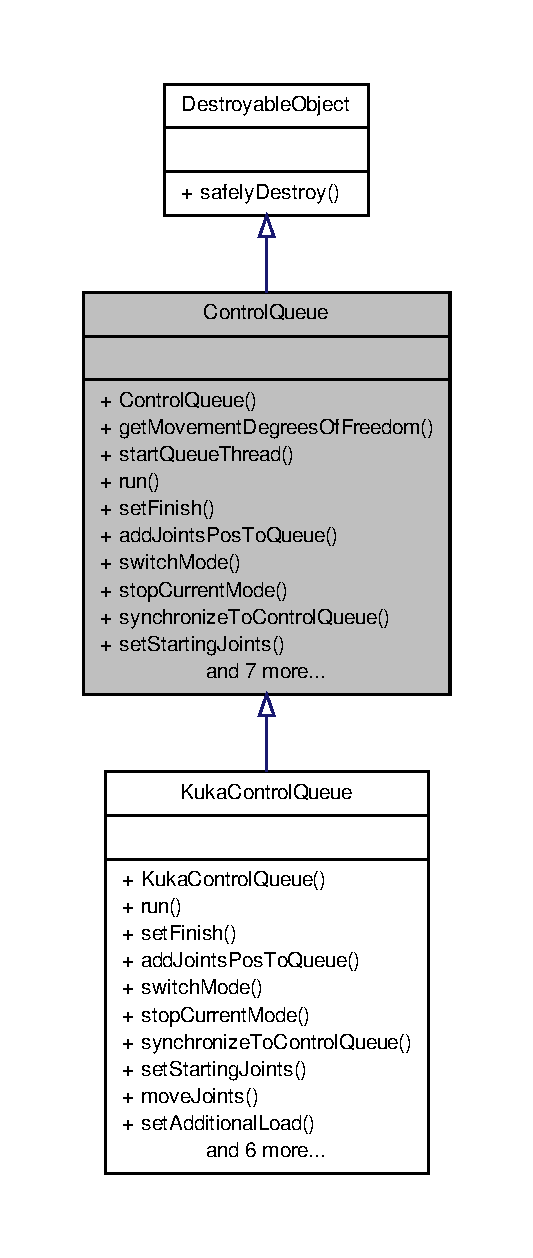
\includegraphics[height=550pt]{classControlQueue__inherit__graph}
\end{center}
\end{figure}


\-Collaboration diagram for \-Control\-Queue\-:\nopagebreak
\begin{figure}[H]
\begin{center}
\leavevmode
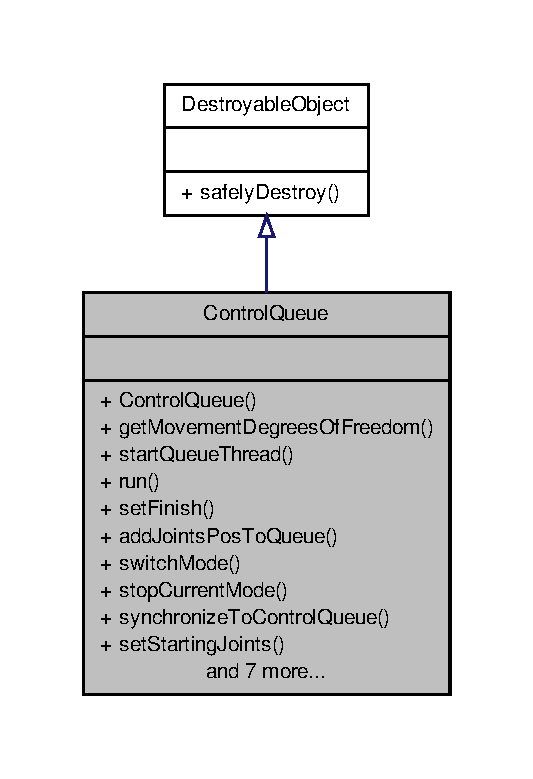
\includegraphics[width=256pt]{classControlQueue__coll__graph}
\end{center}
\end{figure}
\subsection*{\-Public \-Member \-Functions}
\begin{DoxyCompactItemize}
\item 
\hyperlink{classControlQueue_a3a6be1aca489a92e8ff7102e0544de86}{\-Control\-Queue} (int deg\-Of\-Freedom)
\begin{DoxyCompactList}\small\item\em \-Constructor taking the robot dependent degrees of freedom. \end{DoxyCompactList}\item 
int \hyperlink{classControlQueue_aff978436e653dbb2e3de1ca8c7c4a4af}{get\-Movement\-Degrees\-Of\-Freedom} ()
\begin{DoxyCompactList}\small\item\em \-Returns number of robots degrees of freedom. \end{DoxyCompactList}\item 
thread $\ast$ \hyperlink{classControlQueue_ad625c246b5994cb8fab6e59610bc2f40}{start\-Queue\-Thread} ()
\begin{DoxyCompactList}\small\item\em \-Starts new thread to control the robot with real time capability. \end{DoxyCompactList}\item 
virtual void \hyperlink{classControlQueue_a532fc65ff27e37e35078ae2ccc54e408}{run} ()=0
\begin{DoxyCompactList}\small\item\em \-This method is started in a new thread by start\-Queue. \end{DoxyCompactList}\item 
virtual void \hyperlink{classControlQueue_a07626e6ef2bdf7e5fe59a2548ab0a213}{set\-Finish} ()=0
\begin{DoxyCompactList}\small\item\em \-Sets a flag to stop the control thread after current iteration is executed. \end{DoxyCompactList}\item 
virtual void \hyperlink{classControlQueue_a8750612f82e110cb5378672d6f64ca6f}{add\-Joints\-Pos\-To\-Queue} (float $\ast$\hyperlink{fri__example_8m_a094bd681592faefb6f9be3d22d34cbcd}{joints})=0
\begin{DoxyCompactList}\small\item\em \-Adds next joint position to queue. \end{DoxyCompactList}\item 
virtual void \hyperlink{classControlQueue_a0f0367b72b6b1bd75b39aeb19db93dc5}{switch\-Mode} (int mode)=0
\begin{DoxyCompactList}\small\item\em \-Switches robot modes. \-A state might be a real time command mode or an monitoring mode. \end{DoxyCompactList}\item 
virtual void \hyperlink{classControlQueue_a74ed9cbabd7a9f6a62460dbd5dc9e48d}{stop\-Current\-Mode} ()=0
\begin{DoxyCompactList}\small\item\em \-Stops current mode and switches back to default mode (e.\-g. monitoring mode) \end{DoxyCompactList}\item 
virtual void \hyperlink{classControlQueue_a37493f41806df96293a95f52f23da280}{synchronize\-To\-Control\-Queue} (int max\-Num\-Joints\-In\-Queue)=0
\begin{DoxyCompactList}\small\item\em \-Blocks, if more than the defined maximum element count is in the queue. \end{DoxyCompactList}\item 
virtual void \hyperlink{classControlQueue_ad63c9ae478a918b3e60cedbe89f78054}{set\-Starting\-Joints} (float $\ast$\hyperlink{fri__example_8m_a094bd681592faefb6f9be3d22d34cbcd}{joints})=0
\begin{DoxyCompactList}\small\item\em \-Sets joints in which the should be in before robot enters command mode. \end{DoxyCompactList}\item 
virtual void \hyperlink{classControlQueue_ac42d07279bbbf5f72928955ea71a407f}{move\-Joints} (float $\ast$\hyperlink{fri__example_8m_a094bd681592faefb6f9be3d22d34cbcd}{joints})=0
\begin{DoxyCompactList}\small\item\em \-Implements simple point to point movement in joint space. \end{DoxyCompactList}\item 
virtual void \hyperlink{classControlQueue_ae34e58840111692913a45ccde7b6fc20}{set\-Additional\-Load} (float load\-Mass, float load\-Pos)=0
\begin{DoxyCompactList}\small\item\em \-Changes the load data of the robot (e.\-g. needs to be used whenever robot picks up an object) \end{DoxyCompactList}\item 
virtual void \hyperlink{classControlQueue_ad6d5bccd9d08d40d5464f10a958e5328}{set\-Stiffness} (float cpstiffnessxyz, float cpstiffnessabc, float cpdamping, float cpmaxdelta, float maxforce, float axismaxdeltatrq)=0
\begin{DoxyCompactList}\small\item\em \-Sets certain stiffness parameters in cartesian space (if the robot supports this) according to a mass spring damper system model. \end{DoxyCompactList}\item 
virtual float $\ast$ \hyperlink{classControlQueue_a9bdc3efe662d9d275d48ec523627ef7c}{get\-Cartesian\-Pos} ()=0
\begin{DoxyCompactList}\small\item\em \-Returns current robot position in cartesian space. \end{DoxyCompactList}\item 
virtual float $\ast$ \hyperlink{classControlQueue_a4b8c95e38791477bf925ac8f61c38821}{get\-Starting\-Joints} ()=0
\begin{DoxyCompactList}\small\item\em \-Returns the robot joints the robot has been directly before starting command mode. \end{DoxyCompactList}\item 
virtual float $\ast$ \hyperlink{classControlQueue_a7b803a4b12bfa70c79fdad108e63b0f4}{retrieve\-Joints\-From\-Robot} ()=0
\begin{DoxyCompactList}\small\item\em \-Returns joints if the robot is in monitor mode. \end{DoxyCompactList}\item 
virtual mes\-\_\-result \hyperlink{classControlQueue_aa610fa7b8b53ed7c406eba1fa4eb106c}{get\-Current\-Joints} ()=0
\begin{DoxyCompactList}\small\item\em \-Returns joints if the robot is in command mode. \end{DoxyCompactList}\item 
virtual bool \hyperlink{classControlQueue_a153ff04f335b33580d15d2e16f17265b}{is\-Initialized} ()=0
\begin{DoxyCompactList}\small\item\em \-Returns true if the command mode initialization is done. \end{DoxyCompactList}\end{DoxyCompactItemize}


\subsection{\-Detailed \-Description}
\-This class provides a set of methods that are necessary to execute basic manipulations with robots. \-As this typically is a real time task, this class contains a queue and sends data to the robot at specified times. 

\subsection{\-Constructor \& \-Destructor \-Documentation}
\hypertarget{classControlQueue_a3a6be1aca489a92e8ff7102e0544de86}{\index{\-Control\-Queue@{\-Control\-Queue}!\-Control\-Queue@{\-Control\-Queue}}
\index{\-Control\-Queue@{\-Control\-Queue}!ControlQueue@{\-Control\-Queue}}
\subsubsection[{\-Control\-Queue}]{\setlength{\rightskip}{0pt plus 5cm}{\bf \-Control\-Queue\-::\-Control\-Queue} (
\begin{DoxyParamCaption}
\item[{int}]{deg\-Of\-Freedom}
\end{DoxyParamCaption}
)}}\label{classControlQueue_a3a6be1aca489a92e8ff7102e0544de86}

\begin{DoxyParams}{\-Parameters}
{\em deg\-Of\-Freedom} & number of robots degrees of freedom \\
\hline
\end{DoxyParams}


\subsection{\-Member \-Function \-Documentation}
\hypertarget{classControlQueue_a8750612f82e110cb5378672d6f64ca6f}{\index{\-Control\-Queue@{\-Control\-Queue}!add\-Joints\-Pos\-To\-Queue@{add\-Joints\-Pos\-To\-Queue}}
\index{add\-Joints\-Pos\-To\-Queue@{add\-Joints\-Pos\-To\-Queue}!ControlQueue@{\-Control\-Queue}}
\subsubsection[{add\-Joints\-Pos\-To\-Queue}]{\setlength{\rightskip}{0pt plus 5cm}virtual void {\bf \-Control\-Queue\-::add\-Joints\-Pos\-To\-Queue} (
\begin{DoxyParamCaption}
\item[{float $\ast$}]{joints}
\end{DoxyParamCaption}
)\hspace{0.3cm}{\ttfamily  \mbox{[}pure virtual\mbox{]}}}}\label{classControlQueue_a8750612f82e110cb5378672d6f64ca6f}

\begin{DoxyParams}{\-Parameters}
{\em joints} & joints to add \\
\hline
\end{DoxyParams}


\-Implemented in \hyperlink{classKukaControlQueue_a62ccf60f8a53d8d04a14a4d396b3d13a}{\-Kuka\-Control\-Queue}.

\hypertarget{classControlQueue_a9bdc3efe662d9d275d48ec523627ef7c}{\index{\-Control\-Queue@{\-Control\-Queue}!get\-Cartesian\-Pos@{get\-Cartesian\-Pos}}
\index{get\-Cartesian\-Pos@{get\-Cartesian\-Pos}!ControlQueue@{\-Control\-Queue}}
\subsubsection[{get\-Cartesian\-Pos}]{\setlength{\rightskip}{0pt plus 5cm}virtual float$\ast$ {\bf \-Control\-Queue\-::get\-Cartesian\-Pos} (
\begin{DoxyParamCaption}
{}
\end{DoxyParamCaption}
)\hspace{0.3cm}{\ttfamily  \mbox{[}pure virtual\mbox{]}}}}\label{classControlQueue_a9bdc3efe662d9d275d48ec523627ef7c}


\-Implemented in \hyperlink{classKukaControlQueue_a62475e2d6fd485bfbce095d67bab96c6}{\-Kuka\-Control\-Queue}.

\hypertarget{classControlQueue_aa610fa7b8b53ed7c406eba1fa4eb106c}{\index{\-Control\-Queue@{\-Control\-Queue}!get\-Current\-Joints@{get\-Current\-Joints}}
\index{get\-Current\-Joints@{get\-Current\-Joints}!ControlQueue@{\-Control\-Queue}}
\subsubsection[{get\-Current\-Joints}]{\setlength{\rightskip}{0pt plus 5cm}virtual mes\-\_\-result {\bf \-Control\-Queue\-::get\-Current\-Joints} (
\begin{DoxyParamCaption}
{}
\end{DoxyParamCaption}
)\hspace{0.3cm}{\ttfamily  \mbox{[}pure virtual\mbox{]}}}}\label{classControlQueue_aa610fa7b8b53ed7c406eba1fa4eb106c}


\-Implemented in \hyperlink{classKukaControlQueue_a363040926a2e014b347cc7016b639f25}{\-Kuka\-Control\-Queue}.

\hypertarget{classControlQueue_aff978436e653dbb2e3de1ca8c7c4a4af}{\index{\-Control\-Queue@{\-Control\-Queue}!get\-Movement\-Degrees\-Of\-Freedom@{get\-Movement\-Degrees\-Of\-Freedom}}
\index{get\-Movement\-Degrees\-Of\-Freedom@{get\-Movement\-Degrees\-Of\-Freedom}!ControlQueue@{\-Control\-Queue}}
\subsubsection[{get\-Movement\-Degrees\-Of\-Freedom}]{\setlength{\rightskip}{0pt plus 5cm}int {\bf \-Control\-Queue\-::get\-Movement\-Degrees\-Of\-Freedom} (
\begin{DoxyParamCaption}
{}
\end{DoxyParamCaption}
)}}\label{classControlQueue_aff978436e653dbb2e3de1ca8c7c4a4af}
\hypertarget{classControlQueue_a4b8c95e38791477bf925ac8f61c38821}{\index{\-Control\-Queue@{\-Control\-Queue}!get\-Starting\-Joints@{get\-Starting\-Joints}}
\index{get\-Starting\-Joints@{get\-Starting\-Joints}!ControlQueue@{\-Control\-Queue}}
\subsubsection[{get\-Starting\-Joints}]{\setlength{\rightskip}{0pt plus 5cm}virtual float$\ast$ {\bf \-Control\-Queue\-::get\-Starting\-Joints} (
\begin{DoxyParamCaption}
{}
\end{DoxyParamCaption}
)\hspace{0.3cm}{\ttfamily  \mbox{[}pure virtual\mbox{]}}}}\label{classControlQueue_a4b8c95e38791477bf925ac8f61c38821}


\-Implemented in \hyperlink{classKukaControlQueue_a53c5b0fe118ce0847586ccccc1481edb}{\-Kuka\-Control\-Queue}.

\hypertarget{classControlQueue_a153ff04f335b33580d15d2e16f17265b}{\index{\-Control\-Queue@{\-Control\-Queue}!is\-Initialized@{is\-Initialized}}
\index{is\-Initialized@{is\-Initialized}!ControlQueue@{\-Control\-Queue}}
\subsubsection[{is\-Initialized}]{\setlength{\rightskip}{0pt plus 5cm}virtual bool {\bf \-Control\-Queue\-::is\-Initialized} (
\begin{DoxyParamCaption}
{}
\end{DoxyParamCaption}
)\hspace{0.3cm}{\ttfamily  \mbox{[}pure virtual\mbox{]}}}}\label{classControlQueue_a153ff04f335b33580d15d2e16f17265b}


\-Implemented in \hyperlink{classKukaControlQueue_ae7844ed3c8210152dd0b4a97e9c9f7a6}{\-Kuka\-Control\-Queue}.

\hypertarget{classControlQueue_ac42d07279bbbf5f72928955ea71a407f}{\index{\-Control\-Queue@{\-Control\-Queue}!move\-Joints@{move\-Joints}}
\index{move\-Joints@{move\-Joints}!ControlQueue@{\-Control\-Queue}}
\subsubsection[{move\-Joints}]{\setlength{\rightskip}{0pt plus 5cm}virtual void {\bf \-Control\-Queue\-::move\-Joints} (
\begin{DoxyParamCaption}
\item[{float $\ast$}]{joints}
\end{DoxyParamCaption}
)\hspace{0.3cm}{\ttfamily  \mbox{[}pure virtual\mbox{]}}}}\label{classControlQueue_ac42d07279bbbf5f72928955ea71a407f}

\begin{DoxyParams}{\-Parameters}
{\em joints} & array of joint positions \\
\hline
\end{DoxyParams}


\-Implemented in \hyperlink{classKukaControlQueue_a2b9e7cfb4918201e1da5e2a365395e46}{\-Kuka\-Control\-Queue}.

\hypertarget{classControlQueue_a7b803a4b12bfa70c79fdad108e63b0f4}{\index{\-Control\-Queue@{\-Control\-Queue}!retrieve\-Joints\-From\-Robot@{retrieve\-Joints\-From\-Robot}}
\index{retrieve\-Joints\-From\-Robot@{retrieve\-Joints\-From\-Robot}!ControlQueue@{\-Control\-Queue}}
\subsubsection[{retrieve\-Joints\-From\-Robot}]{\setlength{\rightskip}{0pt plus 5cm}virtual float$\ast$ {\bf \-Control\-Queue\-::retrieve\-Joints\-From\-Robot} (
\begin{DoxyParamCaption}
{}
\end{DoxyParamCaption}
)\hspace{0.3cm}{\ttfamily  \mbox{[}pure virtual\mbox{]}}}}\label{classControlQueue_a7b803a4b12bfa70c79fdad108e63b0f4}


\-Implemented in \hyperlink{classKukaControlQueue_a4d426306e965f9e81cdad5b10229866f}{\-Kuka\-Control\-Queue}.

\hypertarget{classControlQueue_a532fc65ff27e37e35078ae2ccc54e408}{\index{\-Control\-Queue@{\-Control\-Queue}!run@{run}}
\index{run@{run}!ControlQueue@{\-Control\-Queue}}
\subsubsection[{run}]{\setlength{\rightskip}{0pt plus 5cm}virtual void {\bf \-Control\-Queue\-::run} (
\begin{DoxyParamCaption}
{}
\end{DoxyParamCaption}
)\hspace{0.3cm}{\ttfamily  \mbox{[}pure virtual\mbox{]}}}}\label{classControlQueue_a532fc65ff27e37e35078ae2ccc54e408}


\-Implemented in \hyperlink{classKukaControlQueue_ac77a50c65dd633fa18913c45cc6fe26a}{\-Kuka\-Control\-Queue}.

\hypertarget{classControlQueue_ae34e58840111692913a45ccde7b6fc20}{\index{\-Control\-Queue@{\-Control\-Queue}!set\-Additional\-Load@{set\-Additional\-Load}}
\index{set\-Additional\-Load@{set\-Additional\-Load}!ControlQueue@{\-Control\-Queue}}
\subsubsection[{set\-Additional\-Load}]{\setlength{\rightskip}{0pt plus 5cm}virtual void {\bf \-Control\-Queue\-::set\-Additional\-Load} (
\begin{DoxyParamCaption}
\item[{float}]{load\-Mass, }
\item[{float}]{load\-Pos}
\end{DoxyParamCaption}
)\hspace{0.3cm}{\ttfamily  \mbox{[}pure virtual\mbox{]}}}}\label{classControlQueue_ae34e58840111692913a45ccde7b6fc20}

\begin{DoxyParams}{\-Parameters}
{\em load\-Mass} & mass of the picked up object \\
\hline
{\em load\-Pos} & position of the objects center of gravity relative to the manipulator \\
\hline
\end{DoxyParams}


\-Implemented in \hyperlink{classKukaControlQueue_a0c6a2edd22e222c672668fac5cacb55a}{\-Kuka\-Control\-Queue}.

\hypertarget{classControlQueue_a07626e6ef2bdf7e5fe59a2548ab0a213}{\index{\-Control\-Queue@{\-Control\-Queue}!set\-Finish@{set\-Finish}}
\index{set\-Finish@{set\-Finish}!ControlQueue@{\-Control\-Queue}}
\subsubsection[{set\-Finish}]{\setlength{\rightskip}{0pt plus 5cm}virtual void {\bf \-Control\-Queue\-::set\-Finish} (
\begin{DoxyParamCaption}
{}
\end{DoxyParamCaption}
)\hspace{0.3cm}{\ttfamily  \mbox{[}pure virtual\mbox{]}}}}\label{classControlQueue_a07626e6ef2bdf7e5fe59a2548ab0a213}


\-Implemented in \hyperlink{classKukaControlQueue_aac151fe8a3fb3e2744ea29ef37036754}{\-Kuka\-Control\-Queue}.

\hypertarget{classControlQueue_ad63c9ae478a918b3e60cedbe89f78054}{\index{\-Control\-Queue@{\-Control\-Queue}!set\-Starting\-Joints@{set\-Starting\-Joints}}
\index{set\-Starting\-Joints@{set\-Starting\-Joints}!ControlQueue@{\-Control\-Queue}}
\subsubsection[{set\-Starting\-Joints}]{\setlength{\rightskip}{0pt plus 5cm}virtual void {\bf \-Control\-Queue\-::set\-Starting\-Joints} (
\begin{DoxyParamCaption}
\item[{float $\ast$}]{joints}
\end{DoxyParamCaption}
)\hspace{0.3cm}{\ttfamily  \mbox{[}pure virtual\mbox{]}}}}\label{classControlQueue_ad63c9ae478a918b3e60cedbe89f78054}

\begin{DoxyParams}{\-Parameters}
{\em joints} & array of joint positions \\
\hline
\end{DoxyParams}


\-Implemented in \hyperlink{classKukaControlQueue_ae9b6465ad4c714b305af4eb0b8e69584}{\-Kuka\-Control\-Queue}.

\hypertarget{classControlQueue_ad6d5bccd9d08d40d5464f10a958e5328}{\index{\-Control\-Queue@{\-Control\-Queue}!set\-Stiffness@{set\-Stiffness}}
\index{set\-Stiffness@{set\-Stiffness}!ControlQueue@{\-Control\-Queue}}
\subsubsection[{set\-Stiffness}]{\setlength{\rightskip}{0pt plus 5cm}virtual void {\bf \-Control\-Queue\-::set\-Stiffness} (
\begin{DoxyParamCaption}
\item[{float}]{cpstiffnessxyz, }
\item[{float}]{cpstiffnessabc, }
\item[{float}]{cpdamping, }
\item[{float}]{cpmaxdelta, }
\item[{float}]{maxforce, }
\item[{float}]{axismaxdeltatrq}
\end{DoxyParamCaption}
)\hspace{0.3cm}{\ttfamily  \mbox{[}pure virtual\mbox{]}}}}\label{classControlQueue_ad6d5bccd9d08d40d5464f10a958e5328}

\begin{DoxyParams}{\-Parameters}
{\em cpstiffnessxyz} & stiffness of the robot in the cartesian space \\
\hline
{\em cpstiffnessabc} & stiffness of the rotational axis of the tool mounting point in cartesian space \\
\hline
{\em cpdamping} & damping of the robots axis in cartesian space \\
\hline
{\em cpmaxdelta} & maximum allows deviation in cartesian space \\
\hline
{\em maxforce} & maximum allowed applied force \\
\hline
{\em axismaxdeltatrq} & maximum allowed applied torque \\
\hline
\end{DoxyParams}


\-Implemented in \hyperlink{classKukaControlQueue_a82c93a4979d678344337461dd9084725}{\-Kuka\-Control\-Queue}.

\hypertarget{classControlQueue_ad625c246b5994cb8fab6e59610bc2f40}{\index{\-Control\-Queue@{\-Control\-Queue}!start\-Queue\-Thread@{start\-Queue\-Thread}}
\index{start\-Queue\-Thread@{start\-Queue\-Thread}!ControlQueue@{\-Control\-Queue}}
\subsubsection[{start\-Queue\-Thread}]{\setlength{\rightskip}{0pt plus 5cm}thread $\ast$ {\bf \-Control\-Queue\-::start\-Queue\-Thread} (
\begin{DoxyParamCaption}
{}
\end{DoxyParamCaption}
)}}\label{classControlQueue_ad625c246b5994cb8fab6e59610bc2f40}
\hypertarget{classControlQueue_a74ed9cbabd7a9f6a62460dbd5dc9e48d}{\index{\-Control\-Queue@{\-Control\-Queue}!stop\-Current\-Mode@{stop\-Current\-Mode}}
\index{stop\-Current\-Mode@{stop\-Current\-Mode}!ControlQueue@{\-Control\-Queue}}
\subsubsection[{stop\-Current\-Mode}]{\setlength{\rightskip}{0pt plus 5cm}virtual void {\bf \-Control\-Queue\-::stop\-Current\-Mode} (
\begin{DoxyParamCaption}
{}
\end{DoxyParamCaption}
)\hspace{0.3cm}{\ttfamily  \mbox{[}pure virtual\mbox{]}}}}\label{classControlQueue_a74ed9cbabd7a9f6a62460dbd5dc9e48d}


\-Implemented in \hyperlink{classKukaControlQueue_a33c03e1a8b1e5fef533a6cdaca9fe15d}{\-Kuka\-Control\-Queue}.

\hypertarget{classControlQueue_a0f0367b72b6b1bd75b39aeb19db93dc5}{\index{\-Control\-Queue@{\-Control\-Queue}!switch\-Mode@{switch\-Mode}}
\index{switch\-Mode@{switch\-Mode}!ControlQueue@{\-Control\-Queue}}
\subsubsection[{switch\-Mode}]{\setlength{\rightskip}{0pt plus 5cm}virtual void {\bf \-Control\-Queue\-::switch\-Mode} (
\begin{DoxyParamCaption}
\item[{int}]{mode}
\end{DoxyParamCaption}
)\hspace{0.3cm}{\ttfamily  \mbox{[}pure virtual\mbox{]}}}}\label{classControlQueue_a0f0367b72b6b1bd75b39aeb19db93dc5}

\begin{DoxyParams}{\-Parameters}
{\em mode} & mode id \\
\hline
\end{DoxyParams}


\-Implemented in \hyperlink{classKukaControlQueue_a8bbf6b7c4a0cea73c4e3891d18d51fdf}{\-Kuka\-Control\-Queue}.

\hypertarget{classControlQueue_a37493f41806df96293a95f52f23da280}{\index{\-Control\-Queue@{\-Control\-Queue}!synchronize\-To\-Control\-Queue@{synchronize\-To\-Control\-Queue}}
\index{synchronize\-To\-Control\-Queue@{synchronize\-To\-Control\-Queue}!ControlQueue@{\-Control\-Queue}}
\subsubsection[{synchronize\-To\-Control\-Queue}]{\setlength{\rightskip}{0pt plus 5cm}virtual void {\bf \-Control\-Queue\-::synchronize\-To\-Control\-Queue} (
\begin{DoxyParamCaption}
\item[{int}]{max\-Num\-Joints\-In\-Queue}
\end{DoxyParamCaption}
)\hspace{0.3cm}{\ttfamily  \mbox{[}pure virtual\mbox{]}}}}\label{classControlQueue_a37493f41806df96293a95f52f23da280}

\begin{DoxyParams}{\-Parameters}
{\em max\-Num\-Joints\-In\-Queue} & maximum number of joints in queue \\
\hline
\end{DoxyParams}


\-Implemented in \hyperlink{classKukaControlQueue_a3e59c3d253d2306b5fdde56da529c9cd}{\-Kuka\-Control\-Queue}.



\-The documentation for this class was generated from the following files\-:\begin{DoxyCompactItemize}
\item 
/home/shangl/data/data\-\_\-synched/studium/informatik/master/master\-\_\-thesis/kukadu\-\_\-framework/thesis/src/robot/\hyperlink{ControlQueue_8h}{\-Control\-Queue.\-h}\item 
/home/shangl/data/data\-\_\-synched/studium/informatik/master/master\-\_\-thesis/kukadu\-\_\-framework/thesis/src/robot/\hyperlink{ControlQueue_8cpp}{\-Control\-Queue.\-cpp}\end{DoxyCompactItemize}

\hypertarget{classCostComputer}{\section{\-Cost\-Computer \-Class \-Reference}
\label{classCostComputer}\index{\-Cost\-Computer@{\-Cost\-Computer}}
}


\-Interface for reinforcement learning cost function computation used by \hyperlink{classDMPReinforcer}{\-D\-M\-P\-Reinforcer}.  




{\ttfamily \#include $<$\-Cost\-Computer.\-h$>$}



\-Inheritance diagram for \-Cost\-Computer\-:\nopagebreak
\begin{figure}[H]
\begin{center}
\leavevmode
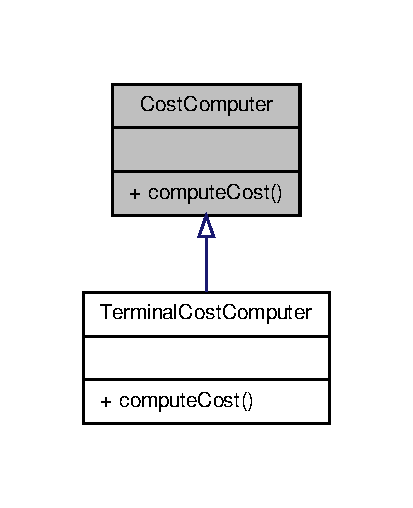
\includegraphics[width=198pt]{classCostComputer__inherit__graph}
\end{center}
\end{figure}
\subsection*{\-Public \-Member \-Functions}
\begin{DoxyCompactItemize}
\item 
virtual double \hyperlink{classCostComputer_a139032631f2d4bd1882d9e5e47960eb0}{compute\-Cost} (t\-\_\-executor\-\_\-res results)=0
\begin{DoxyCompactList}\small\item\em computes cost for a given dmp execution \end{DoxyCompactList}\end{DoxyCompactItemize}


\subsection{\-Detailed \-Description}
\-This class provides the necessary interfaces for the cost function computation 

\subsection{\-Member \-Function \-Documentation}
\hypertarget{classCostComputer_a139032631f2d4bd1882d9e5e47960eb0}{\index{\-Cost\-Computer@{\-Cost\-Computer}!compute\-Cost@{compute\-Cost}}
\index{compute\-Cost@{compute\-Cost}!CostComputer@{\-Cost\-Computer}}
\subsubsection[{compute\-Cost}]{\setlength{\rightskip}{0pt plus 5cm}virtual double {\bf \-Cost\-Computer\-::compute\-Cost} (
\begin{DoxyParamCaption}
\item[{t\-\_\-executor\-\_\-res}]{results}
\end{DoxyParamCaption}
)\hspace{0.3cm}{\ttfamily  \mbox{[}pure virtual\mbox{]}}}}\label{classCostComputer_a139032631f2d4bd1882d9e5e47960eb0}

\begin{DoxyParams}{\-Parameters}
{\em results} & measured results of the last dmp execution \\
\hline
\end{DoxyParams}


\-Implemented in \hyperlink{classTerminalCostComputer_adc77b79cbce50bb7b7b01bf85256d3eb}{\-Terminal\-Cost\-Computer}.



\-The documentation for this class was generated from the following file\-:\begin{DoxyCompactItemize}
\item 
/home/shangl/data/data\-\_\-synched/studium/informatik/master/master\-\_\-thesis/kukadu\-\_\-framework/thesis/src/trajectory/\hyperlink{CostComputer_8h}{\-Cost\-Computer.\-h}\end{DoxyCompactItemize}

\hypertarget{classcSDHOptions}{\section{c\-S\-D\-H\-Options \-Class \-Reference}
\label{classcSDHOptions}\index{c\-S\-D\-H\-Options@{c\-S\-D\-H\-Options}}
}


class for command line option parsing holding option parsing results  




{\ttfamily \#include $<$sdhoptions.\-h$>$}

\subsection*{\-Public \-Member \-Functions}
\begin{DoxyCompactItemize}
\item 
\hyperlink{classcSDHOptions_a855dc504f792a70672dc6e6ce284beac}{c\-S\-D\-H\-Options} (char const $\ast$option\-\_\-selection=\hyperlink{sdhoptions_8h_a90372ef85e86e456fa18741a81f9b81d}{\-S\-D\-H\-U\-S\-A\-G\-E\-\_\-\-D\-E\-F\-A\-U\-L\-T})
\item 
\hyperlink{classcSDHOptions_af6ed7e84c211b5094b2d9c0d18f8a9f7}{$\sim$c\-S\-D\-H\-Options} ()
\begin{DoxyCompactList}\small\item\em destructor, clean up \end{DoxyCompactList}\item 
int \hyperlink{classcSDHOptions_a5424fed1754caa395e0db9638c92323a}{\-Parse} (int argc, char $\ast$$\ast$argv, char const $\ast$helptext, char const $\ast$progname, char const $\ast$version, char const $\ast$libname, char const $\ast$librelease)
\item 
void \hyperlink{classcSDHOptions_a01770c064f4dfe639ad443e8e44c7fb7}{\-Open\-Communication} (\-N\-S\-\_\-\-S\-D\-H c\-S\-D\-H \&hand)
\end{DoxyCompactItemize}
\subsection*{\-Public \-Attributes}
\begin{DoxyCompactItemize}
\item 
std\-::string \hyperlink{classcSDHOptions_a85c5365609e4b34511b81d4c06e6c65c}{usage}
\item 
int \hyperlink{classcSDHOptions_a3cf6556a2758bf431b4e93e5c2adefb7}{debug\-\_\-level}
\item 
std\-::ostream $\ast$ \hyperlink{classcSDHOptions_a71ac0c016aeb7cc34c521d06fa905198}{debuglog}
\item 
int \hyperlink{classcSDHOptions_a565bf00d92a0aca8729c3bd1e0f92be2}{sdhport}
\item 
char \hyperlink{classcSDHOptions_aa33357676ec18be7dbd162e7dac93406}{sdh\-\_\-rs\-\_\-device} \mbox{[}\hyperlink{classcSDHOptions_a9caeb9858b718ed48145a833be2c9178}{\-M\-A\-X\-\_\-\-D\-E\-V\-\_\-\-L\-E\-N\-G\-T\-H}\mbox{]}
\item 
double \hyperlink{classcSDHOptions_a68c00cb00f9ee6a70974ce9c27e4f3d1}{timeout}
\item 
unsigned long \hyperlink{classcSDHOptions_a38c8ae82f4fa578b04d1a9b9fffbe063}{rs232\-\_\-baudrate}
\item 
bool \hyperlink{classcSDHOptions_afa459c797bb8fbb2ad6f45a39261e3d8}{use\-\_\-can\-\_\-esd}
\item 
int \hyperlink{classcSDHOptions_adefa363d3e2c61e37676037a09faaf06}{net}
\item 
bool \hyperlink{classcSDHOptions_ab0b03472ff934016086feaed1cf8d5ea}{use\-\_\-can\-\_\-peak}
\item 
char \hyperlink{classcSDHOptions_acd04aeab5f6ab8e962b739de10bf4d08}{sdh\-\_\-canpeak\-\_\-device} \mbox{[}\hyperlink{classcSDHOptions_a9caeb9858b718ed48145a833be2c9178}{\-M\-A\-X\-\_\-\-D\-E\-V\-\_\-\-L\-E\-N\-G\-T\-H}\mbox{]}
\item 
unsigned long \hyperlink{classcSDHOptions_a2376bfefe00e6f9832c16a979b99bf92}{can\-\_\-baudrate}
\item 
unsigned int \hyperlink{classcSDHOptions_a301e3d6b905c010e82a45420f5cd5634}{id\-\_\-read}
\item 
unsigned int \hyperlink{classcSDHOptions_a3ca7757c9dbb11c190987992582132ab}{id\-\_\-write}
\item 
bool \hyperlink{classcSDHOptions_a484031d2facdcdf2fc3ec9b26df45819}{use\-\_\-radians}
\item 
bool \hyperlink{classcSDHOptions_a6724ffca7223e593e24d74c90a238dab}{use\-\_\-fahrenheit}
\item 
double \hyperlink{classcSDHOptions_a62f70e83e50968e9cdee7b55cff12806}{period}
\item 
int \hyperlink{classcSDHOptions_a0de19c3e4d29f927c9bd8a4071a8e13d}{dsaport}
\item 
char \hyperlink{classcSDHOptions_a8d9d3490f0a39e8982cf9ae4c77f2147}{dsa\-\_\-rs\-\_\-device} \mbox{[}\hyperlink{classcSDHOptions_a9caeb9858b718ed48145a833be2c9178}{\-M\-A\-X\-\_\-\-D\-E\-V\-\_\-\-L\-E\-N\-G\-T\-H}\mbox{]}
\item 
bool \hyperlink{classcSDHOptions_ab285c659c8f86f4dd2c1582f9a5e3608}{do\-\_\-\-R\-L\-E}
\item 
int \hyperlink{classcSDHOptions_a7bdd78ad26a17faeceec15e2431a1c3e}{framerate}
\item 
bool \hyperlink{classcSDHOptions_a9c8cd3c89d1175f2a75afbbb119a7f9b}{fullframe}
\item 
bool \hyperlink{classcSDHOptions_a9ea9c47ffd54eb7a557e672cc76b23d3}{sensorinfo}
\item 
bool \hyperlink{classcSDHOptions_a3e1089848fb7702f5e94dd673601f463}{controllerinfo}
\item 
int \hyperlink{classcSDHOptions_a3dcaa4689b89c3f480cad4744a72c0f8}{matrixinfo} \mbox{[}6\mbox{]}
\item 
double \hyperlink{classcSDHOptions_addfa8552244a84c62fe26ef5c261a19d}{sensitivity} \mbox{[}6\mbox{]}
\item 
unsigned int \hyperlink{classcSDHOptions_abbd91d2dce6cda8d2e4d5103ce44c3c0}{threshold} \mbox{[}6\mbox{]}
\item 
bool \hyperlink{classcSDHOptions_afedb88e59b2ecf58b80c7b0b861ee189}{reset\-\_\-to\-\_\-default}
\item 
bool \hyperlink{classcSDHOptions_aca724e741552d1a6c415abf6a0bf2ecf}{persistent}
\item 
bool \hyperlink{classcSDHOptions_a73021f34d61c57f5991490b8dda9b557}{showdsasettings}
\item 
bool \hyperlink{classcSDHOptions_a57533df7afeb116231686a59bc86a5cd}{use\-\_\-tcp}
\item 
std\-::string \hyperlink{classcSDHOptions_a247c378f5874482d97343fc6c0e577be}{tcp\-\_\-adr}
\item 
int \hyperlink{classcSDHOptions_a8c7190b3d89ec6ff659d171e59fe5f45}{tcp\-\_\-port}
\end{DoxyCompactItemize}
\subsection*{\-Static \-Public \-Attributes}
\begin{DoxyCompactItemize}
\item 
static int const \hyperlink{classcSDHOptions_a9caeb9858b718ed48145a833be2c9178}{\-M\-A\-X\-\_\-\-D\-E\-V\-\_\-\-L\-E\-N\-G\-T\-H} = 32
\end{DoxyCompactItemize}


\subsection{\-Constructor \& \-Destructor \-Documentation}
\hypertarget{classcSDHOptions_a855dc504f792a70672dc6e6ce284beac}{\index{c\-S\-D\-H\-Options@{c\-S\-D\-H\-Options}!c\-S\-D\-H\-Options@{c\-S\-D\-H\-Options}}
\index{c\-S\-D\-H\-Options@{c\-S\-D\-H\-Options}!cSDHOptions@{c\-S\-D\-H\-Options}}
\subsubsection[{c\-S\-D\-H\-Options}]{\setlength{\rightskip}{0pt plus 5cm}{\bf c\-S\-D\-H\-Options\-::c\-S\-D\-H\-Options} (
\begin{DoxyParamCaption}
\item[{char const $\ast$}]{option\-\_\-selection = {\ttfamily {\bf \-S\-D\-H\-U\-S\-A\-G\-E\-\_\-\-D\-E\-F\-A\-U\-L\-T}}}
\end{DoxyParamCaption}
)}}\label{classcSDHOptions_a855dc504f792a70672dc6e6ce284beac}
constructor\-: init members to their default values


\begin{DoxyParams}{\-Parameters}
{\em option\-\_\-selection} & -\/ string that names the options to include in helptext for online help. \-With a text including one of the following keywords the corresponding helptext is added to the usage helptext
\begin{DoxyItemize}
\item \char`\"{}general\char`\"{} see sdhusage\-\_\-general
\item \char`\"{}sdhcom\-\_\-serial\char`\"{} see sdhusage\-\_\-sdhcom\-\_\-serial
\item \char`\"{}sdhcom\-\_\-common\char`\"{} see sdhusage\-\_\-sdhcom\-\_\-common
\item \char`\"{}sdhcom\-\_\-esdcan\char`\"{} see sdhusage\-\_\-sdhcom\-\_\-esdcan
\item \char`\"{}sdhcom\-\_\-peakcan\char`\"{} see sdhusage\-\_\-sdhcom\-\_\-peakcan
\item \char`\"{}sdhcom\-\_\-cancommon\char`\"{} see sdhusage\-\_\-sdhcom\-\_\-cancommon
\item \char`\"{}sdhcom\-\_\-tcp\char`\"{} see sdhusage\-\_\-sdhcom\-\_\-tcp
\item \char`\"{}sdhother\char`\"{} see sdhusage\-\_\-sdhother
\item \char`\"{}dsacom\char`\"{} see sdhusage\-\_\-dsacom
\item \char`\"{}dsaother\char`\"{} see sdhusage\-\_\-dsaother 
\end{DoxyItemize}\\
\hline
\end{DoxyParams}
\hypertarget{classcSDHOptions_af6ed7e84c211b5094b2d9c0d18f8a9f7}{\index{c\-S\-D\-H\-Options@{c\-S\-D\-H\-Options}!$\sim$c\-S\-D\-H\-Options@{$\sim$c\-S\-D\-H\-Options}}
\index{$\sim$c\-S\-D\-H\-Options@{$\sim$c\-S\-D\-H\-Options}!cSDHOptions@{c\-S\-D\-H\-Options}}
\subsubsection[{$\sim$c\-S\-D\-H\-Options}]{\setlength{\rightskip}{0pt plus 5cm}{\bf c\-S\-D\-H\-Options\-::$\sim$c\-S\-D\-H\-Options} (
\begin{DoxyParamCaption}
{}
\end{DoxyParamCaption}
)}}\label{classcSDHOptions_af6ed7e84c211b5094b2d9c0d18f8a9f7}


\subsection{\-Member \-Function \-Documentation}
\hypertarget{classcSDHOptions_a01770c064f4dfe639ad443e8e44c7fb7}{\index{c\-S\-D\-H\-Options@{c\-S\-D\-H\-Options}!\-Open\-Communication@{\-Open\-Communication}}
\index{\-Open\-Communication@{\-Open\-Communication}!cSDHOptions@{c\-S\-D\-H\-Options}}
\subsubsection[{\-Open\-Communication}]{\setlength{\rightskip}{0pt plus 5cm}void {\bf c\-S\-D\-H\-Options\-::\-Open\-Communication} (
\begin{DoxyParamCaption}
\item[{\-N\-S\-\_\-\-S\-D\-H c\-S\-D\-H \&}]{hand}
\end{DoxyParamCaption}
)}}\label{classcSDHOptions_a01770c064f4dfe639ad443e8e44c7fb7}
convenience function to open the communication of the given {\itshape hand\/} object according to the parsed parameters.


\begin{DoxyParams}{\-Parameters}
{\em hand} & -\/ reference to a c\-S\-D\-H object to open \\
\hline
\end{DoxyParams}
\hypertarget{classcSDHOptions_a5424fed1754caa395e0db9638c92323a}{\index{c\-S\-D\-H\-Options@{c\-S\-D\-H\-Options}!\-Parse@{\-Parse}}
\index{\-Parse@{\-Parse}!cSDHOptions@{c\-S\-D\-H\-Options}}
\subsubsection[{\-Parse}]{\setlength{\rightskip}{0pt plus 5cm}int {\bf c\-S\-D\-H\-Options\-::\-Parse} (
\begin{DoxyParamCaption}
\item[{int}]{argc, }
\item[{char $\ast$$\ast$}]{argv, }
\item[{char const $\ast$}]{helptext, }
\item[{char const $\ast$}]{progname, }
\item[{char const $\ast$}]{version, }
\item[{char const $\ast$}]{libname, }
\item[{char const $\ast$}]{librelease}
\end{DoxyParamCaption}
)}}\label{classcSDHOptions_a5424fed1754caa395e0db9638c92323a}
parse the command line parameters {\itshape argc\/}, {\itshape argv\/} into members. {\itshape helptext\/}, {\itshape progname\/}, {\itshape version\/}, {\itshape libname\/} and {\itshape librelease\/} are used when printing online help. start parsing at option with index $\ast$p\-\_\-option\-\_\-index parse all options if parse\-\_\-all is true, else only one option is parsed

\begin{DoxyReturn}{\-Returns}
the optind index of the first non option argument in argv 
\end{DoxyReturn}


\subsection{\-Member \-Data \-Documentation}
\hypertarget{classcSDHOptions_a2376bfefe00e6f9832c16a979b99bf92}{\index{c\-S\-D\-H\-Options@{c\-S\-D\-H\-Options}!can\-\_\-baudrate@{can\-\_\-baudrate}}
\index{can\-\_\-baudrate@{can\-\_\-baudrate}!cSDHOptions@{c\-S\-D\-H\-Options}}
\subsubsection[{can\-\_\-baudrate}]{\setlength{\rightskip}{0pt plus 5cm}unsigned long {\bf c\-S\-D\-H\-Options\-::can\-\_\-baudrate}}}\label{classcSDHOptions_a2376bfefe00e6f9832c16a979b99bf92}
\hypertarget{classcSDHOptions_a3e1089848fb7702f5e94dd673601f463}{\index{c\-S\-D\-H\-Options@{c\-S\-D\-H\-Options}!controllerinfo@{controllerinfo}}
\index{controllerinfo@{controllerinfo}!cSDHOptions@{c\-S\-D\-H\-Options}}
\subsubsection[{controllerinfo}]{\setlength{\rightskip}{0pt plus 5cm}bool {\bf c\-S\-D\-H\-Options\-::controllerinfo}}}\label{classcSDHOptions_a3e1089848fb7702f5e94dd673601f463}
\hypertarget{classcSDHOptions_a3cf6556a2758bf431b4e93e5c2adefb7}{\index{c\-S\-D\-H\-Options@{c\-S\-D\-H\-Options}!debug\-\_\-level@{debug\-\_\-level}}
\index{debug\-\_\-level@{debug\-\_\-level}!cSDHOptions@{c\-S\-D\-H\-Options}}
\subsubsection[{debug\-\_\-level}]{\setlength{\rightskip}{0pt plus 5cm}int {\bf c\-S\-D\-H\-Options\-::debug\-\_\-level}}}\label{classcSDHOptions_a3cf6556a2758bf431b4e93e5c2adefb7}
\hypertarget{classcSDHOptions_a71ac0c016aeb7cc34c521d06fa905198}{\index{c\-S\-D\-H\-Options@{c\-S\-D\-H\-Options}!debuglog@{debuglog}}
\index{debuglog@{debuglog}!cSDHOptions@{c\-S\-D\-H\-Options}}
\subsubsection[{debuglog}]{\setlength{\rightskip}{0pt plus 5cm}std\-::ostream$\ast$ {\bf c\-S\-D\-H\-Options\-::debuglog}}}\label{classcSDHOptions_a71ac0c016aeb7cc34c521d06fa905198}
\hypertarget{classcSDHOptions_ab285c659c8f86f4dd2c1582f9a5e3608}{\index{c\-S\-D\-H\-Options@{c\-S\-D\-H\-Options}!do\-\_\-\-R\-L\-E@{do\-\_\-\-R\-L\-E}}
\index{do\-\_\-\-R\-L\-E@{do\-\_\-\-R\-L\-E}!cSDHOptions@{c\-S\-D\-H\-Options}}
\subsubsection[{do\-\_\-\-R\-L\-E}]{\setlength{\rightskip}{0pt plus 5cm}bool {\bf c\-S\-D\-H\-Options\-::do\-\_\-\-R\-L\-E}}}\label{classcSDHOptions_ab285c659c8f86f4dd2c1582f9a5e3608}
\hypertarget{classcSDHOptions_a8d9d3490f0a39e8982cf9ae4c77f2147}{\index{c\-S\-D\-H\-Options@{c\-S\-D\-H\-Options}!dsa\-\_\-rs\-\_\-device@{dsa\-\_\-rs\-\_\-device}}
\index{dsa\-\_\-rs\-\_\-device@{dsa\-\_\-rs\-\_\-device}!cSDHOptions@{c\-S\-D\-H\-Options}}
\subsubsection[{dsa\-\_\-rs\-\_\-device}]{\setlength{\rightskip}{0pt plus 5cm}char {\bf c\-S\-D\-H\-Options\-::dsa\-\_\-rs\-\_\-device}\mbox{[}{\bf \-M\-A\-X\-\_\-\-D\-E\-V\-\_\-\-L\-E\-N\-G\-T\-H}\mbox{]}}}\label{classcSDHOptions_a8d9d3490f0a39e8982cf9ae4c77f2147}
\hypertarget{classcSDHOptions_a0de19c3e4d29f927c9bd8a4071a8e13d}{\index{c\-S\-D\-H\-Options@{c\-S\-D\-H\-Options}!dsaport@{dsaport}}
\index{dsaport@{dsaport}!cSDHOptions@{c\-S\-D\-H\-Options}}
\subsubsection[{dsaport}]{\setlength{\rightskip}{0pt plus 5cm}int {\bf c\-S\-D\-H\-Options\-::dsaport}}}\label{classcSDHOptions_a0de19c3e4d29f927c9bd8a4071a8e13d}
\hypertarget{classcSDHOptions_a7bdd78ad26a17faeceec15e2431a1c3e}{\index{c\-S\-D\-H\-Options@{c\-S\-D\-H\-Options}!framerate@{framerate}}
\index{framerate@{framerate}!cSDHOptions@{c\-S\-D\-H\-Options}}
\subsubsection[{framerate}]{\setlength{\rightskip}{0pt plus 5cm}int {\bf c\-S\-D\-H\-Options\-::framerate}}}\label{classcSDHOptions_a7bdd78ad26a17faeceec15e2431a1c3e}
\hypertarget{classcSDHOptions_a9c8cd3c89d1175f2a75afbbb119a7f9b}{\index{c\-S\-D\-H\-Options@{c\-S\-D\-H\-Options}!fullframe@{fullframe}}
\index{fullframe@{fullframe}!cSDHOptions@{c\-S\-D\-H\-Options}}
\subsubsection[{fullframe}]{\setlength{\rightskip}{0pt plus 5cm}bool {\bf c\-S\-D\-H\-Options\-::fullframe}}}\label{classcSDHOptions_a9c8cd3c89d1175f2a75afbbb119a7f9b}
\hypertarget{classcSDHOptions_a301e3d6b905c010e82a45420f5cd5634}{\index{c\-S\-D\-H\-Options@{c\-S\-D\-H\-Options}!id\-\_\-read@{id\-\_\-read}}
\index{id\-\_\-read@{id\-\_\-read}!cSDHOptions@{c\-S\-D\-H\-Options}}
\subsubsection[{id\-\_\-read}]{\setlength{\rightskip}{0pt plus 5cm}unsigned int {\bf c\-S\-D\-H\-Options\-::id\-\_\-read}}}\label{classcSDHOptions_a301e3d6b905c010e82a45420f5cd5634}
\hypertarget{classcSDHOptions_a3ca7757c9dbb11c190987992582132ab}{\index{c\-S\-D\-H\-Options@{c\-S\-D\-H\-Options}!id\-\_\-write@{id\-\_\-write}}
\index{id\-\_\-write@{id\-\_\-write}!cSDHOptions@{c\-S\-D\-H\-Options}}
\subsubsection[{id\-\_\-write}]{\setlength{\rightskip}{0pt plus 5cm}unsigned int {\bf c\-S\-D\-H\-Options\-::id\-\_\-write}}}\label{classcSDHOptions_a3ca7757c9dbb11c190987992582132ab}
\hypertarget{classcSDHOptions_a3dcaa4689b89c3f480cad4744a72c0f8}{\index{c\-S\-D\-H\-Options@{c\-S\-D\-H\-Options}!matrixinfo@{matrixinfo}}
\index{matrixinfo@{matrixinfo}!cSDHOptions@{c\-S\-D\-H\-Options}}
\subsubsection[{matrixinfo}]{\setlength{\rightskip}{0pt plus 5cm}int {\bf c\-S\-D\-H\-Options\-::matrixinfo}\mbox{[}6\mbox{]}}}\label{classcSDHOptions_a3dcaa4689b89c3f480cad4744a72c0f8}
\hypertarget{classcSDHOptions_a9caeb9858b718ed48145a833be2c9178}{\index{c\-S\-D\-H\-Options@{c\-S\-D\-H\-Options}!\-M\-A\-X\-\_\-\-D\-E\-V\-\_\-\-L\-E\-N\-G\-T\-H@{\-M\-A\-X\-\_\-\-D\-E\-V\-\_\-\-L\-E\-N\-G\-T\-H}}
\index{\-M\-A\-X\-\_\-\-D\-E\-V\-\_\-\-L\-E\-N\-G\-T\-H@{\-M\-A\-X\-\_\-\-D\-E\-V\-\_\-\-L\-E\-N\-G\-T\-H}!cSDHOptions@{c\-S\-D\-H\-Options}}
\subsubsection[{\-M\-A\-X\-\_\-\-D\-E\-V\-\_\-\-L\-E\-N\-G\-T\-H}]{\setlength{\rightskip}{0pt plus 5cm}int const {\bf c\-S\-D\-H\-Options\-::\-M\-A\-X\-\_\-\-D\-E\-V\-\_\-\-L\-E\-N\-G\-T\-H} = 32\hspace{0.3cm}{\ttfamily  \mbox{[}static\mbox{]}}}}\label{classcSDHOptions_a9caeb9858b718ed48145a833be2c9178}
\hypertarget{classcSDHOptions_adefa363d3e2c61e37676037a09faaf06}{\index{c\-S\-D\-H\-Options@{c\-S\-D\-H\-Options}!net@{net}}
\index{net@{net}!cSDHOptions@{c\-S\-D\-H\-Options}}
\subsubsection[{net}]{\setlength{\rightskip}{0pt plus 5cm}int {\bf c\-S\-D\-H\-Options\-::net}}}\label{classcSDHOptions_adefa363d3e2c61e37676037a09faaf06}
\hypertarget{classcSDHOptions_a62f70e83e50968e9cdee7b55cff12806}{\index{c\-S\-D\-H\-Options@{c\-S\-D\-H\-Options}!period@{period}}
\index{period@{period}!cSDHOptions@{c\-S\-D\-H\-Options}}
\subsubsection[{period}]{\setlength{\rightskip}{0pt plus 5cm}double {\bf c\-S\-D\-H\-Options\-::period}}}\label{classcSDHOptions_a62f70e83e50968e9cdee7b55cff12806}
\hypertarget{classcSDHOptions_aca724e741552d1a6c415abf6a0bf2ecf}{\index{c\-S\-D\-H\-Options@{c\-S\-D\-H\-Options}!persistent@{persistent}}
\index{persistent@{persistent}!cSDHOptions@{c\-S\-D\-H\-Options}}
\subsubsection[{persistent}]{\setlength{\rightskip}{0pt plus 5cm}bool {\bf c\-S\-D\-H\-Options\-::persistent}}}\label{classcSDHOptions_aca724e741552d1a6c415abf6a0bf2ecf}
\hypertarget{classcSDHOptions_afedb88e59b2ecf58b80c7b0b861ee189}{\index{c\-S\-D\-H\-Options@{c\-S\-D\-H\-Options}!reset\-\_\-to\-\_\-default@{reset\-\_\-to\-\_\-default}}
\index{reset\-\_\-to\-\_\-default@{reset\-\_\-to\-\_\-default}!cSDHOptions@{c\-S\-D\-H\-Options}}
\subsubsection[{reset\-\_\-to\-\_\-default}]{\setlength{\rightskip}{0pt plus 5cm}bool {\bf c\-S\-D\-H\-Options\-::reset\-\_\-to\-\_\-default}}}\label{classcSDHOptions_afedb88e59b2ecf58b80c7b0b861ee189}
\hypertarget{classcSDHOptions_a38c8ae82f4fa578b04d1a9b9fffbe063}{\index{c\-S\-D\-H\-Options@{c\-S\-D\-H\-Options}!rs232\-\_\-baudrate@{rs232\-\_\-baudrate}}
\index{rs232\-\_\-baudrate@{rs232\-\_\-baudrate}!cSDHOptions@{c\-S\-D\-H\-Options}}
\subsubsection[{rs232\-\_\-baudrate}]{\setlength{\rightskip}{0pt plus 5cm}unsigned long {\bf c\-S\-D\-H\-Options\-::rs232\-\_\-baudrate}}}\label{classcSDHOptions_a38c8ae82f4fa578b04d1a9b9fffbe063}
\hypertarget{classcSDHOptions_acd04aeab5f6ab8e962b739de10bf4d08}{\index{c\-S\-D\-H\-Options@{c\-S\-D\-H\-Options}!sdh\-\_\-canpeak\-\_\-device@{sdh\-\_\-canpeak\-\_\-device}}
\index{sdh\-\_\-canpeak\-\_\-device@{sdh\-\_\-canpeak\-\_\-device}!cSDHOptions@{c\-S\-D\-H\-Options}}
\subsubsection[{sdh\-\_\-canpeak\-\_\-device}]{\setlength{\rightskip}{0pt plus 5cm}char {\bf c\-S\-D\-H\-Options\-::sdh\-\_\-canpeak\-\_\-device}\mbox{[}{\bf \-M\-A\-X\-\_\-\-D\-E\-V\-\_\-\-L\-E\-N\-G\-T\-H}\mbox{]}}}\label{classcSDHOptions_acd04aeab5f6ab8e962b739de10bf4d08}
\hypertarget{classcSDHOptions_aa33357676ec18be7dbd162e7dac93406}{\index{c\-S\-D\-H\-Options@{c\-S\-D\-H\-Options}!sdh\-\_\-rs\-\_\-device@{sdh\-\_\-rs\-\_\-device}}
\index{sdh\-\_\-rs\-\_\-device@{sdh\-\_\-rs\-\_\-device}!cSDHOptions@{c\-S\-D\-H\-Options}}
\subsubsection[{sdh\-\_\-rs\-\_\-device}]{\setlength{\rightskip}{0pt plus 5cm}char {\bf c\-S\-D\-H\-Options\-::sdh\-\_\-rs\-\_\-device}\mbox{[}{\bf \-M\-A\-X\-\_\-\-D\-E\-V\-\_\-\-L\-E\-N\-G\-T\-H}\mbox{]}}}\label{classcSDHOptions_aa33357676ec18be7dbd162e7dac93406}
\hypertarget{classcSDHOptions_a565bf00d92a0aca8729c3bd1e0f92be2}{\index{c\-S\-D\-H\-Options@{c\-S\-D\-H\-Options}!sdhport@{sdhport}}
\index{sdhport@{sdhport}!cSDHOptions@{c\-S\-D\-H\-Options}}
\subsubsection[{sdhport}]{\setlength{\rightskip}{0pt plus 5cm}int {\bf c\-S\-D\-H\-Options\-::sdhport}}}\label{classcSDHOptions_a565bf00d92a0aca8729c3bd1e0f92be2}
\hypertarget{classcSDHOptions_addfa8552244a84c62fe26ef5c261a19d}{\index{c\-S\-D\-H\-Options@{c\-S\-D\-H\-Options}!sensitivity@{sensitivity}}
\index{sensitivity@{sensitivity}!cSDHOptions@{c\-S\-D\-H\-Options}}
\subsubsection[{sensitivity}]{\setlength{\rightskip}{0pt plus 5cm}double {\bf c\-S\-D\-H\-Options\-::sensitivity}\mbox{[}6\mbox{]}}}\label{classcSDHOptions_addfa8552244a84c62fe26ef5c261a19d}
\hypertarget{classcSDHOptions_a9ea9c47ffd54eb7a557e672cc76b23d3}{\index{c\-S\-D\-H\-Options@{c\-S\-D\-H\-Options}!sensorinfo@{sensorinfo}}
\index{sensorinfo@{sensorinfo}!cSDHOptions@{c\-S\-D\-H\-Options}}
\subsubsection[{sensorinfo}]{\setlength{\rightskip}{0pt plus 5cm}bool {\bf c\-S\-D\-H\-Options\-::sensorinfo}}}\label{classcSDHOptions_a9ea9c47ffd54eb7a557e672cc76b23d3}
\hypertarget{classcSDHOptions_a73021f34d61c57f5991490b8dda9b557}{\index{c\-S\-D\-H\-Options@{c\-S\-D\-H\-Options}!showdsasettings@{showdsasettings}}
\index{showdsasettings@{showdsasettings}!cSDHOptions@{c\-S\-D\-H\-Options}}
\subsubsection[{showdsasettings}]{\setlength{\rightskip}{0pt plus 5cm}bool {\bf c\-S\-D\-H\-Options\-::showdsasettings}}}\label{classcSDHOptions_a73021f34d61c57f5991490b8dda9b557}
\hypertarget{classcSDHOptions_a247c378f5874482d97343fc6c0e577be}{\index{c\-S\-D\-H\-Options@{c\-S\-D\-H\-Options}!tcp\-\_\-adr@{tcp\-\_\-adr}}
\index{tcp\-\_\-adr@{tcp\-\_\-adr}!cSDHOptions@{c\-S\-D\-H\-Options}}
\subsubsection[{tcp\-\_\-adr}]{\setlength{\rightskip}{0pt plus 5cm}std\-::string {\bf c\-S\-D\-H\-Options\-::tcp\-\_\-adr}}}\label{classcSDHOptions_a247c378f5874482d97343fc6c0e577be}
\hypertarget{classcSDHOptions_a8c7190b3d89ec6ff659d171e59fe5f45}{\index{c\-S\-D\-H\-Options@{c\-S\-D\-H\-Options}!tcp\-\_\-port@{tcp\-\_\-port}}
\index{tcp\-\_\-port@{tcp\-\_\-port}!cSDHOptions@{c\-S\-D\-H\-Options}}
\subsubsection[{tcp\-\_\-port}]{\setlength{\rightskip}{0pt plus 5cm}int {\bf c\-S\-D\-H\-Options\-::tcp\-\_\-port}}}\label{classcSDHOptions_a8c7190b3d89ec6ff659d171e59fe5f45}
\hypertarget{classcSDHOptions_abbd91d2dce6cda8d2e4d5103ce44c3c0}{\index{c\-S\-D\-H\-Options@{c\-S\-D\-H\-Options}!threshold@{threshold}}
\index{threshold@{threshold}!cSDHOptions@{c\-S\-D\-H\-Options}}
\subsubsection[{threshold}]{\setlength{\rightskip}{0pt plus 5cm}unsigned int {\bf c\-S\-D\-H\-Options\-::threshold}\mbox{[}6\mbox{]}}}\label{classcSDHOptions_abbd91d2dce6cda8d2e4d5103ce44c3c0}
\hypertarget{classcSDHOptions_a68c00cb00f9ee6a70974ce9c27e4f3d1}{\index{c\-S\-D\-H\-Options@{c\-S\-D\-H\-Options}!timeout@{timeout}}
\index{timeout@{timeout}!cSDHOptions@{c\-S\-D\-H\-Options}}
\subsubsection[{timeout}]{\setlength{\rightskip}{0pt plus 5cm}double {\bf c\-S\-D\-H\-Options\-::timeout}}}\label{classcSDHOptions_a68c00cb00f9ee6a70974ce9c27e4f3d1}
\hypertarget{classcSDHOptions_a85c5365609e4b34511b81d4c06e6c65c}{\index{c\-S\-D\-H\-Options@{c\-S\-D\-H\-Options}!usage@{usage}}
\index{usage@{usage}!cSDHOptions@{c\-S\-D\-H\-Options}}
\subsubsection[{usage}]{\setlength{\rightskip}{0pt plus 5cm}std\-::string {\bf c\-S\-D\-H\-Options\-::usage}}}\label{classcSDHOptions_a85c5365609e4b34511b81d4c06e6c65c}
\hypertarget{classcSDHOptions_afa459c797bb8fbb2ad6f45a39261e3d8}{\index{c\-S\-D\-H\-Options@{c\-S\-D\-H\-Options}!use\-\_\-can\-\_\-esd@{use\-\_\-can\-\_\-esd}}
\index{use\-\_\-can\-\_\-esd@{use\-\_\-can\-\_\-esd}!cSDHOptions@{c\-S\-D\-H\-Options}}
\subsubsection[{use\-\_\-can\-\_\-esd}]{\setlength{\rightskip}{0pt plus 5cm}bool {\bf c\-S\-D\-H\-Options\-::use\-\_\-can\-\_\-esd}}}\label{classcSDHOptions_afa459c797bb8fbb2ad6f45a39261e3d8}
\hypertarget{classcSDHOptions_ab0b03472ff934016086feaed1cf8d5ea}{\index{c\-S\-D\-H\-Options@{c\-S\-D\-H\-Options}!use\-\_\-can\-\_\-peak@{use\-\_\-can\-\_\-peak}}
\index{use\-\_\-can\-\_\-peak@{use\-\_\-can\-\_\-peak}!cSDHOptions@{c\-S\-D\-H\-Options}}
\subsubsection[{use\-\_\-can\-\_\-peak}]{\setlength{\rightskip}{0pt plus 5cm}bool {\bf c\-S\-D\-H\-Options\-::use\-\_\-can\-\_\-peak}}}\label{classcSDHOptions_ab0b03472ff934016086feaed1cf8d5ea}
\hypertarget{classcSDHOptions_a6724ffca7223e593e24d74c90a238dab}{\index{c\-S\-D\-H\-Options@{c\-S\-D\-H\-Options}!use\-\_\-fahrenheit@{use\-\_\-fahrenheit}}
\index{use\-\_\-fahrenheit@{use\-\_\-fahrenheit}!cSDHOptions@{c\-S\-D\-H\-Options}}
\subsubsection[{use\-\_\-fahrenheit}]{\setlength{\rightskip}{0pt plus 5cm}bool {\bf c\-S\-D\-H\-Options\-::use\-\_\-fahrenheit}}}\label{classcSDHOptions_a6724ffca7223e593e24d74c90a238dab}
\hypertarget{classcSDHOptions_a484031d2facdcdf2fc3ec9b26df45819}{\index{c\-S\-D\-H\-Options@{c\-S\-D\-H\-Options}!use\-\_\-radians@{use\-\_\-radians}}
\index{use\-\_\-radians@{use\-\_\-radians}!cSDHOptions@{c\-S\-D\-H\-Options}}
\subsubsection[{use\-\_\-radians}]{\setlength{\rightskip}{0pt plus 5cm}bool {\bf c\-S\-D\-H\-Options\-::use\-\_\-radians}}}\label{classcSDHOptions_a484031d2facdcdf2fc3ec9b26df45819}
\hypertarget{classcSDHOptions_a57533df7afeb116231686a59bc86a5cd}{\index{c\-S\-D\-H\-Options@{c\-S\-D\-H\-Options}!use\-\_\-tcp@{use\-\_\-tcp}}
\index{use\-\_\-tcp@{use\-\_\-tcp}!cSDHOptions@{c\-S\-D\-H\-Options}}
\subsubsection[{use\-\_\-tcp}]{\setlength{\rightskip}{0pt plus 5cm}bool {\bf c\-S\-D\-H\-Options\-::use\-\_\-tcp}}}\label{classcSDHOptions_a57533df7afeb116231686a59bc86a5cd}


\-The documentation for this class was generated from the following files\-:\begin{DoxyCompactItemize}
\item 
/home/shangl/data/data\-\_\-synched/studium/informatik/master/master\-\_\-thesis/kukadu\-\_\-framework/thesis/src/robot/mounted/\hyperlink{sdhoptions_8h}{sdhoptions.\-h}\item 
/home/shangl/data/data\-\_\-synched/studium/informatik/master/master\-\_\-thesis/kukadu\-\_\-framework/thesis/src/robot/mounted/\hyperlink{sdhoptions_8cpp}{sdhoptions.\-cpp}\end{DoxyCompactItemize}

\hypertarget{classDestroyableObject}{\section{\-Destroyable\-Object \-Class \-Reference}
\label{classDestroyableObject}\index{\-Destroyable\-Object@{\-Destroyable\-Object}}
}


\-Interface defining a callback function.  




{\ttfamily \#include $<$\-Destroyable\-Object.\-h$>$}



\-Inheritance diagram for \-Destroyable\-Object\-:\nopagebreak
\begin{figure}[H]
\begin{center}
\leavevmode
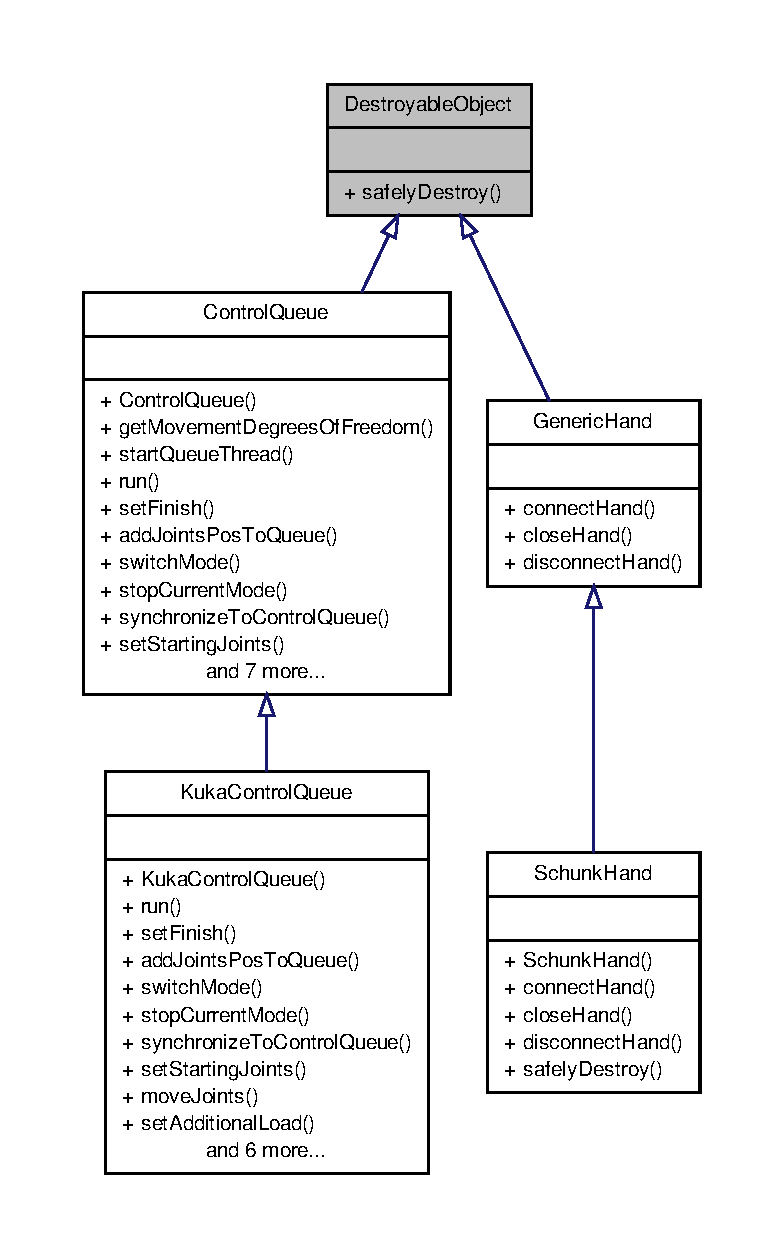
\includegraphics[height=550pt]{classDestroyableObject__inherit__graph}
\end{center}
\end{figure}
\subsection*{\-Public \-Member \-Functions}
\begin{DoxyCompactItemize}
\item 
virtual void \hyperlink{classDestroyableObject_a728d19d81eca540efd68650867f197be}{safely\-Destroy} ()=0
\begin{DoxyCompactList}\small\item\em \-Method is called whenever destroy event occurs and ensures safe and clean termination of the programm (e.\-g. stops robot) \end{DoxyCompactList}\end{DoxyCompactItemize}


\subsection{\-Detailed \-Description}
\-The specified callback function should be called whenever unexpected behaviour during robot execution occurs. \-This is used to handle this execption in a controlled way. 

\subsection{\-Member \-Function \-Documentation}
\hypertarget{classDestroyableObject_a728d19d81eca540efd68650867f197be}{\index{\-Destroyable\-Object@{\-Destroyable\-Object}!safely\-Destroy@{safely\-Destroy}}
\index{safely\-Destroy@{safely\-Destroy}!DestroyableObject@{\-Destroyable\-Object}}
\subsubsection[{safely\-Destroy}]{\setlength{\rightskip}{0pt plus 5cm}virtual void {\bf \-Destroyable\-Object\-::safely\-Destroy} (
\begin{DoxyParamCaption}
{}
\end{DoxyParamCaption}
)\hspace{0.3cm}{\ttfamily  \mbox{[}pure virtual\mbox{]}}}}\label{classDestroyableObject_a728d19d81eca540efd68650867f197be}


\-Implemented in \hyperlink{classKukaControlQueue_ad086a60270e8c6b56c3e09aa1c595b4e}{\-Kuka\-Control\-Queue}, and \hyperlink{classSchunkHand_a2d1e10b2b14e293edcf84100b07116cc}{\-Schunk\-Hand}.



\-The documentation for this class was generated from the following file\-:\begin{DoxyCompactItemize}
\item 
/home/shangl/data/data\-\_\-synched/studium/informatik/master/master\-\_\-thesis/kukadu\-\_\-framework/thesis/src/utils/\hyperlink{DestroyableObject_8h}{\-Destroyable\-Object.\-h}\end{DoxyCompactItemize}

\hypertarget{classDMPExecutor}{\section{\-D\-M\-P\-Executor \-Class \-Reference}
\label{classDMPExecutor}\index{\-D\-M\-P\-Executor@{\-D\-M\-P\-Executor}}
}


\-This class is responsible for dmp execution.  




{\ttfamily \#include $<$\-D\-M\-P\-Executor.\-h$>$}

\subsection*{\-Public \-Member \-Functions}
\begin{DoxyCompactItemize}
\item 
\hyperlink{classDMPExecutor_af5b812ae01ae17b1f82e01af41f2a7f5}{\-D\-M\-P\-Executor} (struct t\-\_\-learned\-\_\-dmp dmp)
\begin{DoxyCompactList}\small\item\em constructor \end{DoxyCompactList}\item 
t\-\_\-executor\-\_\-res \hyperlink{classDMPExecutor_a879428006706b25f5da2109b0608b41e}{simulate\-D\-M\-P} (double t\-Start, double t\-End, double step\-Size, double tol\-Abs\-Err, double tol\-Rel\-Err)
\begin{DoxyCompactList}\small\item\em simulates the dmp \end{DoxyCompactList}\item 
t\-\_\-executor\-\_\-res \hyperlink{classDMPExecutor_a532d85a4a83bec2c28b6c15518b10927}{run\-D\-M\-P} (double ac, double t\-Start, double t\-End, double step\-Size, double tol\-Abs\-Err, double tol\-Rel\-Err, \hyperlink{classControlQueue}{\-Control\-Queue} $\ast$control\-Queue)
\begin{DoxyCompactList}\small\item\em executes the dmp on a robot \end{DoxyCompactList}\end{DoxyCompactItemize}
\subsection*{\-Protected \-Member \-Functions}
\begin{DoxyCompactItemize}
\item 
int \hyperlink{classDMPExecutor_a2e2f614c8f2242136dbcfcb4178d34d4}{func} (double t, const double $\ast$y, double $\ast$f, void $\ast$params)
\item 
int \hyperlink{classDMPExecutor_a228de59529572c211a66e7b7321cacda}{jac} (double t, const double $\ast$y, double $\ast$dfdy, double $\ast$dfdt, void $\ast$params)
\end{DoxyCompactItemize}


\subsection{\-Detailed \-Description}
\-The \hyperlink{classDMPExecutor}{\-D\-M\-P\-Executor} computes the evolution of the dynmic movement primitives by using a numerical differential equation solver. \-It provides execution and simulation mode. \-If the execution mode is selected, a control queue has to be passed to constructor. 

\subsection{\-Constructor \& \-Destructor \-Documentation}
\hypertarget{classDMPExecutor_af5b812ae01ae17b1f82e01af41f2a7f5}{\index{\-D\-M\-P\-Executor@{\-D\-M\-P\-Executor}!\-D\-M\-P\-Executor@{\-D\-M\-P\-Executor}}
\index{\-D\-M\-P\-Executor@{\-D\-M\-P\-Executor}!DMPExecutor@{\-D\-M\-P\-Executor}}
\subsubsection[{\-D\-M\-P\-Executor}]{\setlength{\rightskip}{0pt plus 5cm}{\bf \-D\-M\-P\-Executor\-::\-D\-M\-P\-Executor} (
\begin{DoxyParamCaption}
\item[{struct t\-\_\-learned\-\_\-dmp}]{dmp}
\end{DoxyParamCaption}
)}}\label{classDMPExecutor_af5b812ae01ae17b1f82e01af41f2a7f5}

\begin{DoxyParams}{\-Parameters}
{\em dmp} & the dmp that should be executed \\
\hline
\end{DoxyParams}


\subsection{\-Member \-Function \-Documentation}
\hypertarget{classDMPExecutor_a2e2f614c8f2242136dbcfcb4178d34d4}{\index{\-D\-M\-P\-Executor@{\-D\-M\-P\-Executor}!func@{func}}
\index{func@{func}!DMPExecutor@{\-D\-M\-P\-Executor}}
\subsubsection[{func}]{\setlength{\rightskip}{0pt plus 5cm}int {\bf \-D\-M\-P\-Executor\-::func} (
\begin{DoxyParamCaption}
\item[{double}]{t, }
\item[{const double $\ast$}]{y, }
\item[{double $\ast$}]{f, }
\item[{void $\ast$}]{params}
\end{DoxyParamCaption}
)\hspace{0.3cm}{\ttfamily  \mbox{[}protected\mbox{]}}}}\label{classDMPExecutor_a2e2f614c8f2242136dbcfcb4178d34d4}
\hypertarget{classDMPExecutor_a228de59529572c211a66e7b7321cacda}{\index{\-D\-M\-P\-Executor@{\-D\-M\-P\-Executor}!jac@{jac}}
\index{jac@{jac}!DMPExecutor@{\-D\-M\-P\-Executor}}
\subsubsection[{jac}]{\setlength{\rightskip}{0pt plus 5cm}int {\bf \-D\-M\-P\-Executor\-::jac} (
\begin{DoxyParamCaption}
\item[{double}]{t, }
\item[{const double $\ast$}]{y, }
\item[{double $\ast$}]{dfdy, }
\item[{double $\ast$}]{dfdt, }
\item[{void $\ast$}]{params}
\end{DoxyParamCaption}
)\hspace{0.3cm}{\ttfamily  \mbox{[}protected\mbox{]}}}}\label{classDMPExecutor_a228de59529572c211a66e7b7321cacda}
\hypertarget{classDMPExecutor_a532d85a4a83bec2c28b6c15518b10927}{\index{\-D\-M\-P\-Executor@{\-D\-M\-P\-Executor}!run\-D\-M\-P@{run\-D\-M\-P}}
\index{run\-D\-M\-P@{run\-D\-M\-P}!DMPExecutor@{\-D\-M\-P\-Executor}}
\subsubsection[{run\-D\-M\-P}]{\setlength{\rightskip}{0pt plus 5cm}t\-\_\-executor\-\_\-res {\bf \-D\-M\-P\-Executor\-::run\-D\-M\-P} (
\begin{DoxyParamCaption}
\item[{double}]{ac, }
\item[{double}]{t\-Start, }
\item[{double}]{t\-End, }
\item[{double}]{step\-Size, }
\item[{double}]{tol\-Abs\-Err, }
\item[{double}]{tol\-Rel\-Err, }
\item[{{\bf \-Control\-Queue} $\ast$}]{control\-Queue}
\end{DoxyParamCaption}
)}}\label{classDMPExecutor_a532d85a4a83bec2c28b6c15518b10927}

\begin{DoxyParams}{\-Parameters}
{\em ac} & phase stopping parameter \\
\hline
{\em t\-Start} & start position of the dmp execution (should be typically 0) \\
\hline
{\em t\-End} & end time of the dmp execution \\
\hline
{\em step\-Size} & defines the time interval \\
\hline
{\em tol\-Abs\-Err} & maximum of absolute tolerated error for differential equation solver \\
\hline
{\em tol\-Rel\-Err} & maximum of relative tolerated error for differential equation solver \\
\hline
{\em control\-Queue} & control queue needed for robot execution \\
\hline
\end{DoxyParams}
\hypertarget{classDMPExecutor_a879428006706b25f5da2109b0608b41e}{\index{\-D\-M\-P\-Executor@{\-D\-M\-P\-Executor}!simulate\-D\-M\-P@{simulate\-D\-M\-P}}
\index{simulate\-D\-M\-P@{simulate\-D\-M\-P}!DMPExecutor@{\-D\-M\-P\-Executor}}
\subsubsection[{simulate\-D\-M\-P}]{\setlength{\rightskip}{0pt plus 5cm}t\-\_\-executor\-\_\-res {\bf \-D\-M\-P\-Executor\-::simulate\-D\-M\-P} (
\begin{DoxyParamCaption}
\item[{double}]{t\-Start, }
\item[{double}]{t\-End, }
\item[{double}]{step\-Size, }
\item[{double}]{tol\-Abs\-Err, }
\item[{double}]{tol\-Rel\-Err}
\end{DoxyParamCaption}
)}}\label{classDMPExecutor_a879428006706b25f5da2109b0608b41e}

\begin{DoxyParams}{\-Parameters}
{\em t\-Start} & start position of the dmp execution (should be typically 0) \\
\hline
{\em t\-End} & end time of the dmp execution \\
\hline
{\em step\-Size} & defines the time interval \\
\hline
{\em tol\-Abs\-Err} & maximum of absolute tolerated error for differential equation solver \\
\hline
{\em tol\-Rel\-Err} & maximum of relative tolerated error for differential equation solver \\
\hline
\end{DoxyParams}


\-The documentation for this class was generated from the following files\-:\begin{DoxyCompactItemize}
\item 
/home/shangl/data/data\-\_\-synched/studium/informatik/master/master\-\_\-thesis/kukadu\-\_\-framework/thesis/src/trajectory/\hyperlink{DMPExecutor_8h}{\-D\-M\-P\-Executor.\-h}\item 
/home/shangl/data/data\-\_\-synched/studium/informatik/master/master\-\_\-thesis/kukadu\-\_\-framework/thesis/src/trajectory/\hyperlink{DMPExecutor_8cpp}{\-D\-M\-P\-Executor.\-cpp}\end{DoxyCompactItemize}

\hypertarget{classDMPGeneralizer}{\section{\-D\-M\-P\-Generalizer \-Class \-Reference}
\label{classDMPGeneralizer}\index{\-D\-M\-P\-Generalizer@{\-D\-M\-P\-Generalizer}}
}


\-This class is able to generalize task specific trajectories from previous examples.  




{\ttfamily \#include $<$\-D\-M\-P\-Generalizer.\-h$>$}

\subsection*{\-Public \-Member \-Functions}
\begin{DoxyCompactItemize}
\item 
\hyperlink{classDMPGeneralizer_a303eae31baa6a2c7b897c0fc23a8686c}{\-D\-M\-P\-Generalizer} (string base\-Folder, int deg\-Of\-Freedom, vector$<$ double $>$ tmpmys, vector$<$ double $>$ tmpsigmas, double az, double bz)
\begin{DoxyCompactList}\small\item\em constructor \end{DoxyCompactList}\item 
int \hyperlink{classDMPGeneralizer_a879e11ed7717071401af84c6a42a7bf2}{get\-Query\-Point\-Count} ()
\begin{DoxyCompactList}\small\item\em returns number of trajectory samples \end{DoxyCompactList}\item 
t\-\_\-querypoint \hyperlink{classDMPGeneralizer_a6e725b20d17d60f1851d4c812a0afa92}{get\-Query\-Point\-By\-Index} (int index)
\begin{DoxyCompactList}\small\item\em returns a sample point by index \end{DoxyCompactList}\item 
t\-\_\-learned\-\_\-dmp \hyperlink{classDMPGeneralizer_a1abc5c3749209d570467042757b5c462}{generalize\-Dmp} (\hyperlink{classGenericKernel}{\-Generic\-Kernel} $\ast$trajectory\-Kernel, \hyperlink{classGenericKernel}{\-Generic\-Kernel} $\ast$parameter\-Kernel, vec query, double beta)
\begin{DoxyCompactList}\small\item\em returns the generalized trajectory at a certain query point \end{DoxyCompactList}\end{DoxyCompactItemize}


\subsection{\-Detailed \-Description}
\-This method works well on tasks, where the sample trajectories are similar in shape. \-Therefore, several simple trajectories have to be measured and stored in files. 

\subsection{\-Constructor \& \-Destructor \-Documentation}
\hypertarget{classDMPGeneralizer_a303eae31baa6a2c7b897c0fc23a8686c}{\index{\-D\-M\-P\-Generalizer@{\-D\-M\-P\-Generalizer}!\-D\-M\-P\-Generalizer@{\-D\-M\-P\-Generalizer}}
\index{\-D\-M\-P\-Generalizer@{\-D\-M\-P\-Generalizer}!DMPGeneralizer@{\-D\-M\-P\-Generalizer}}
\subsubsection[{\-D\-M\-P\-Generalizer}]{\setlength{\rightskip}{0pt plus 5cm}{\bf \-D\-M\-P\-Generalizer\-::\-D\-M\-P\-Generalizer} (
\begin{DoxyParamCaption}
\item[{string}]{base\-Folder, }
\item[{int}]{deg\-Of\-Freedom, }
\item[{vector$<$ double $>$}]{tmpmys, }
\item[{vector$<$ double $>$}]{tmpsigmas, }
\item[{double}]{az, }
\item[{double}]{bz}
\end{DoxyParamCaption}
)}}\label{classDMPGeneralizer_a303eae31baa6a2c7b897c0fc23a8686c}

\begin{DoxyParams}{\-Parameters}
{\em base\-Folder} & folder that contains the sample trajectory files \\
\hline
{\em deg\-Of\-Freedom} & number of degrees of freedom \\
\hline
{\em tmpmys} & defines basis functions for dynamic movement primitives \\
\hline
{\em tmpsigmas} & defines basis functions for dynamic movement primitives \\
\hline
{\em az} & dmp az parameter \\
\hline
{\em bz} & dmp bz parameter \\
\hline
\end{DoxyParams}


\subsection{\-Member \-Function \-Documentation}
\hypertarget{classDMPGeneralizer_a1abc5c3749209d570467042757b5c462}{\index{\-D\-M\-P\-Generalizer@{\-D\-M\-P\-Generalizer}!generalize\-Dmp@{generalize\-Dmp}}
\index{generalize\-Dmp@{generalize\-Dmp}!DMPGeneralizer@{\-D\-M\-P\-Generalizer}}
\subsubsection[{generalize\-Dmp}]{\setlength{\rightskip}{0pt plus 5cm}t\-\_\-learned\-\_\-dmp {\bf \-D\-M\-P\-Generalizer\-::generalize\-Dmp} (
\begin{DoxyParamCaption}
\item[{{\bf \-Generic\-Kernel} $\ast$}]{trajectory\-Kernel, }
\item[{{\bf \-Generic\-Kernel} $\ast$}]{parameter\-Kernel, }
\item[{vec}]{query, }
\item[{double}]{beta}
\end{DoxyParamCaption}
)}}\label{classDMPGeneralizer_a1abc5c3749209d570467042757b5c462}

\begin{DoxyParams}{\-Parameters}
{\em trajectory\-Kernel} & kernel for trajectory shape generalization \\
\hline
{\em parameter\-Kernel} & kernel for trajectory goal generalization \\
\hline
{\em query} & required query point \\
\hline
{\em beta} & beta for \-Gaussian processes \\
\hline
\end{DoxyParams}
\hypertarget{classDMPGeneralizer_a6e725b20d17d60f1851d4c812a0afa92}{\index{\-D\-M\-P\-Generalizer@{\-D\-M\-P\-Generalizer}!get\-Query\-Point\-By\-Index@{get\-Query\-Point\-By\-Index}}
\index{get\-Query\-Point\-By\-Index@{get\-Query\-Point\-By\-Index}!DMPGeneralizer@{\-D\-M\-P\-Generalizer}}
\subsubsection[{get\-Query\-Point\-By\-Index}]{\setlength{\rightskip}{0pt plus 5cm}t\-\_\-querypoint {\bf \-D\-M\-P\-Generalizer\-::get\-Query\-Point\-By\-Index} (
\begin{DoxyParamCaption}
\item[{int}]{index}
\end{DoxyParamCaption}
)}}\label{classDMPGeneralizer_a6e725b20d17d60f1851d4c812a0afa92}

\begin{DoxyParams}{\-Parameters}
{\em index} & index of sample point \\
\hline
\end{DoxyParams}
\hypertarget{classDMPGeneralizer_a879e11ed7717071401af84c6a42a7bf2}{\index{\-D\-M\-P\-Generalizer@{\-D\-M\-P\-Generalizer}!get\-Query\-Point\-Count@{get\-Query\-Point\-Count}}
\index{get\-Query\-Point\-Count@{get\-Query\-Point\-Count}!DMPGeneralizer@{\-D\-M\-P\-Generalizer}}
\subsubsection[{get\-Query\-Point\-Count}]{\setlength{\rightskip}{0pt plus 5cm}int {\bf \-D\-M\-P\-Generalizer\-::get\-Query\-Point\-Count} (
\begin{DoxyParamCaption}
{}
\end{DoxyParamCaption}
)}}\label{classDMPGeneralizer_a879e11ed7717071401af84c6a42a7bf2}


\-The documentation for this class was generated from the following files\-:\begin{DoxyCompactItemize}
\item 
/home/shangl/data/data\-\_\-synched/studium/informatik/master/master\-\_\-thesis/kukadu\-\_\-framework/thesis/src/trajectory/\hyperlink{DMPGeneralizer_8h}{\-D\-M\-P\-Generalizer.\-h}\item 
/home/shangl/data/data\-\_\-synched/studium/informatik/master/master\-\_\-thesis/kukadu\-\_\-framework/thesis/src/trajectory/\hyperlink{DMPGeneralizer_8cpp}{\-D\-M\-P\-Generalizer.\-cpp}\end{DoxyCompactItemize}

\hypertarget{classDMPReinforcer}{\section{\-D\-M\-P\-Reinforcer \-Class \-Reference}
\label{classDMPReinforcer}\index{\-D\-M\-P\-Reinforcer@{\-D\-M\-P\-Reinforcer}}
}


\-The \hyperlink{classDMPReinforcer}{\-D\-M\-P\-Reinforcer} provides a general framework for reinforcement learning.  




{\ttfamily \#include $<$\-D\-M\-P\-Reinforcer.\-h$>$}



\-Inheritance diagram for \-D\-M\-P\-Reinforcer\-:
\nopagebreak
\begin{figure}[H]
\begin{center}
\leavevmode
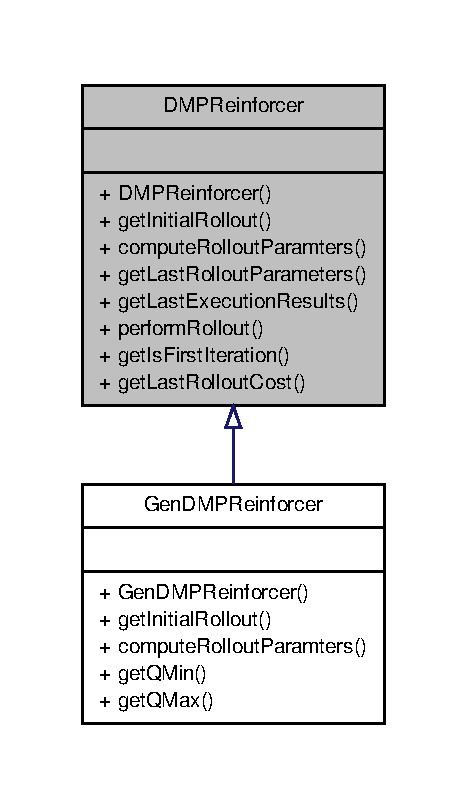
\includegraphics[width=224pt]{classDMPReinforcer__inherit__graph}
\end{center}
\end{figure}
\subsection*{\-Public \-Member \-Functions}
\begin{DoxyCompactItemize}
\item 
\hyperlink{classDMPReinforcer_a3360619f6e4f33d9ed9600165cf1c587}{\-D\-M\-P\-Reinforcer} (\hyperlink{classCostComputer}{\-Cost\-Computer} $\ast$cost, \hyperlink{classControlQueue}{\-Control\-Queue} $\ast$movement\-Queue, double ac, double dmp\-Step\-Size, double tol\-Abs\-Err, double tol\-Rel\-Err)
\begin{DoxyCompactList}\small\item\em constructor \end{DoxyCompactList}\item 
virtual t\-\_\-learned\-\_\-dmp \hyperlink{classDMPReinforcer_aa9459e4d8a500cc6851e19a804680db7}{get\-Initial\-Rollout} ()=0
\begin{DoxyCompactList}\small\item\em returns the first rollout of the reinforcement learning algorithm \end{DoxyCompactList}\item 
virtual t\-\_\-learned\-\_\-dmp \hyperlink{classDMPReinforcer_a0c82b35d96fe07663187b8befd5c1042}{compute\-Rollout\-Paramters} ()=0
\begin{DoxyCompactList}\small\item\em computes the dmp parameters for the next rollout \end{DoxyCompactList}\item 
t\-\_\-learned\-\_\-dmp \hyperlink{classDMPReinforcer_a78c7e984f751de8ec4c0c3f6958c21c9}{get\-Last\-Rollout\-Parameters} ()
\item 
t\-\_\-executor\-\_\-res \hyperlink{classDMPReinforcer_aca3f8c0cdcc83587e46afc60dbda26e6}{get\-Last\-Execution\-Results} ()
\item 
void \hyperlink{classDMPReinforcer_a62083811b2610a623f7d3fe8e7fadeee}{perform\-Rollout} (int do\-Simulation, int do\-Execution)
\begin{DoxyCompactList}\small\item\em executes rollout. first, the trajectory is simulated and the user is asked, whether the trajectory really should be executed \end{DoxyCompactList}\item 
bool \hyperlink{classDMPReinforcer_a3ab981755e30c3feb310e020ab705c3d}{get\-Is\-First\-Iteration} ()
\begin{DoxyCompactList}\small\item\em returns true if the first iteration has not been performed yet \end{DoxyCompactList}\item 
double \hyperlink{classDMPReinforcer_a93dbd9ce2b2de8b527dde3039854ace4}{get\-Last\-Rollout\-Cost} ()
\begin{DoxyCompactList}\small\item\em returns cost for the last executed rollout \end{DoxyCompactList}\end{DoxyCompactItemize}


\subsection{\-Detailed \-Description}
\-It is an abstract class that implements elementary functionality that should be in common for all reinforcement learning methods (such as rollout execution). \-A concrete implementation of the \hyperlink{classDMPReinforcer}{\-D\-M\-P\-Reinforcer} has to implement the missing parts such as the methods get\-Initial\-Rollout and compute\-Rollout\-Paramters. 

\subsection{\-Constructor \& \-Destructor \-Documentation}
\hypertarget{classDMPReinforcer_a3360619f6e4f33d9ed9600165cf1c587}{\index{\-D\-M\-P\-Reinforcer@{\-D\-M\-P\-Reinforcer}!\-D\-M\-P\-Reinforcer@{\-D\-M\-P\-Reinforcer}}
\index{\-D\-M\-P\-Reinforcer@{\-D\-M\-P\-Reinforcer}!DMPReinforcer@{\-D\-M\-P\-Reinforcer}}
\subsubsection[{\-D\-M\-P\-Reinforcer}]{\setlength{\rightskip}{0pt plus 5cm}{\bf \-D\-M\-P\-Reinforcer\-::\-D\-M\-P\-Reinforcer} (
\begin{DoxyParamCaption}
\item[{{\bf \-Cost\-Computer} $\ast$}]{cost, }
\item[{{\bf \-Control\-Queue} $\ast$}]{movement\-Queue, }
\item[{double}]{ac, }
\item[{double}]{dmp\-Step\-Size, }
\item[{double}]{tol\-Abs\-Err, }
\item[{double}]{tol\-Rel\-Err}
\end{DoxyParamCaption}
)}}\label{classDMPReinforcer_a3360619f6e4f33d9ed9600165cf1c587}

\begin{DoxyParams}{\-Parameters}
{\em cost} & \hyperlink{classCostComputer}{\-Cost\-Computer} instance that computes the cost of a given rollout \\
\hline
{\em movement\-Queue} & \hyperlink{classControlQueue}{\-Control\-Queue} instance for robot execution \\
\hline
{\em ac} & dmp phase stopping parameter \\
\hline
{\em dmp\-Step\-Size} & step size for dmp execution \\
\hline
{\em tol\-Abs\-Err} & absolute tolerated error for numerical approximation \\
\hline
{\em tol\-Rel\-Err} & relative tolerated error for numerical approximation \\
\hline
\end{DoxyParams}


\subsection{\-Member \-Function \-Documentation}
\hypertarget{classDMPReinforcer_a0c82b35d96fe07663187b8befd5c1042}{\index{\-D\-M\-P\-Reinforcer@{\-D\-M\-P\-Reinforcer}!compute\-Rollout\-Paramters@{compute\-Rollout\-Paramters}}
\index{compute\-Rollout\-Paramters@{compute\-Rollout\-Paramters}!DMPReinforcer@{\-D\-M\-P\-Reinforcer}}
\subsubsection[{compute\-Rollout\-Paramters}]{\setlength{\rightskip}{0pt plus 5cm}virtual t\-\_\-learned\-\_\-dmp {\bf \-D\-M\-P\-Reinforcer\-::compute\-Rollout\-Paramters} (
\begin{DoxyParamCaption}
{}
\end{DoxyParamCaption}
)\hspace{0.3cm}{\ttfamily  \mbox{[}pure virtual\mbox{]}}}}\label{classDMPReinforcer_a0c82b35d96fe07663187b8befd5c1042}


\-Implemented in \hyperlink{classGenDMPReinforcer_aace5aaa5519a64a33f05b0fd95ac0b6e}{\-Gen\-D\-M\-P\-Reinforcer}.

\hypertarget{classDMPReinforcer_aa9459e4d8a500cc6851e19a804680db7}{\index{\-D\-M\-P\-Reinforcer@{\-D\-M\-P\-Reinforcer}!get\-Initial\-Rollout@{get\-Initial\-Rollout}}
\index{get\-Initial\-Rollout@{get\-Initial\-Rollout}!DMPReinforcer@{\-D\-M\-P\-Reinforcer}}
\subsubsection[{get\-Initial\-Rollout}]{\setlength{\rightskip}{0pt plus 5cm}virtual t\-\_\-learned\-\_\-dmp {\bf \-D\-M\-P\-Reinforcer\-::get\-Initial\-Rollout} (
\begin{DoxyParamCaption}
{}
\end{DoxyParamCaption}
)\hspace{0.3cm}{\ttfamily  \mbox{[}pure virtual\mbox{]}}}}\label{classDMPReinforcer_aa9459e4d8a500cc6851e19a804680db7}


\-Implemented in \hyperlink{classGenDMPReinforcer_adf7e9353b54e429649fb5dd5dd17c28e}{\-Gen\-D\-M\-P\-Reinforcer}.

\hypertarget{classDMPReinforcer_a3ab981755e30c3feb310e020ab705c3d}{\index{\-D\-M\-P\-Reinforcer@{\-D\-M\-P\-Reinforcer}!get\-Is\-First\-Iteration@{get\-Is\-First\-Iteration}}
\index{get\-Is\-First\-Iteration@{get\-Is\-First\-Iteration}!DMPReinforcer@{\-D\-M\-P\-Reinforcer}}
\subsubsection[{get\-Is\-First\-Iteration}]{\setlength{\rightskip}{0pt plus 5cm}bool {\bf \-D\-M\-P\-Reinforcer\-::get\-Is\-First\-Iteration} (
\begin{DoxyParamCaption}
{}
\end{DoxyParamCaption}
)}}\label{classDMPReinforcer_a3ab981755e30c3feb310e020ab705c3d}
\hypertarget{classDMPReinforcer_aca3f8c0cdcc83587e46afc60dbda26e6}{\index{\-D\-M\-P\-Reinforcer@{\-D\-M\-P\-Reinforcer}!get\-Last\-Execution\-Results@{get\-Last\-Execution\-Results}}
\index{get\-Last\-Execution\-Results@{get\-Last\-Execution\-Results}!DMPReinforcer@{\-D\-M\-P\-Reinforcer}}
\subsubsection[{get\-Last\-Execution\-Results}]{\setlength{\rightskip}{0pt plus 5cm}t\-\_\-executor\-\_\-res {\bf \-D\-M\-P\-Reinforcer\-::get\-Last\-Execution\-Results} (
\begin{DoxyParamCaption}
{}
\end{DoxyParamCaption}
)}}\label{classDMPReinforcer_aca3f8c0cdcc83587e46afc60dbda26e6}
\hypertarget{classDMPReinforcer_a93dbd9ce2b2de8b527dde3039854ace4}{\index{\-D\-M\-P\-Reinforcer@{\-D\-M\-P\-Reinforcer}!get\-Last\-Rollout\-Cost@{get\-Last\-Rollout\-Cost}}
\index{get\-Last\-Rollout\-Cost@{get\-Last\-Rollout\-Cost}!DMPReinforcer@{\-D\-M\-P\-Reinforcer}}
\subsubsection[{get\-Last\-Rollout\-Cost}]{\setlength{\rightskip}{0pt plus 5cm}double {\bf \-D\-M\-P\-Reinforcer\-::get\-Last\-Rollout\-Cost} (
\begin{DoxyParamCaption}
{}
\end{DoxyParamCaption}
)}}\label{classDMPReinforcer_a93dbd9ce2b2de8b527dde3039854ace4}
\hypertarget{classDMPReinforcer_a78c7e984f751de8ec4c0c3f6958c21c9}{\index{\-D\-M\-P\-Reinforcer@{\-D\-M\-P\-Reinforcer}!get\-Last\-Rollout\-Parameters@{get\-Last\-Rollout\-Parameters}}
\index{get\-Last\-Rollout\-Parameters@{get\-Last\-Rollout\-Parameters}!DMPReinforcer@{\-D\-M\-P\-Reinforcer}}
\subsubsection[{get\-Last\-Rollout\-Parameters}]{\setlength{\rightskip}{0pt plus 5cm}t\-\_\-learned\-\_\-dmp {\bf \-D\-M\-P\-Reinforcer\-::get\-Last\-Rollout\-Parameters} (
\begin{DoxyParamCaption}
{}
\end{DoxyParamCaption}
)}}\label{classDMPReinforcer_a78c7e984f751de8ec4c0c3f6958c21c9}
\hypertarget{classDMPReinforcer_a62083811b2610a623f7d3fe8e7fadeee}{\index{\-D\-M\-P\-Reinforcer@{\-D\-M\-P\-Reinforcer}!perform\-Rollout@{perform\-Rollout}}
\index{perform\-Rollout@{perform\-Rollout}!DMPReinforcer@{\-D\-M\-P\-Reinforcer}}
\subsubsection[{perform\-Rollout}]{\setlength{\rightskip}{0pt plus 5cm}void {\bf \-D\-M\-P\-Reinforcer\-::perform\-Rollout} (
\begin{DoxyParamCaption}
\item[{int}]{do\-Simulation, }
\item[{int}]{do\-Execution}
\end{DoxyParamCaption}
)}}\label{classDMPReinforcer_a62083811b2610a623f7d3fe8e7fadeee}

\begin{DoxyParams}{\-Parameters}
{\em do\-Simulation} & flag whether trajectory should be simulated \\
\hline
{\em do\-Execution} & flag whether trajectory should be executed at robot \\
\hline
\end{DoxyParams}


\-The documentation for this class was generated from the following files\-:\begin{DoxyCompactItemize}
\item 
/home/shangl/data/data\-\_\-synched/studium/informatik/master/master\-\_\-thesis/kukadu\-\_\-framework/thesis/src/trajectory/\hyperlink{DMPReinforcer_8h}{\-D\-M\-P\-Reinforcer.\-h}\item 
/home/shangl/data/data\-\_\-synched/studium/informatik/master/master\-\_\-thesis/kukadu\-\_\-framework/thesis/src/trajectory/\hyperlink{DMPReinforcer_8cpp}{\-D\-M\-P\-Reinforcer.\-cpp}\end{DoxyCompactItemize}

\hypertarget{classDMPTrajectoryGenerator}{\section{\-D\-M\-P\-Trajectory\-Generator \-Class \-Reference}
\label{classDMPTrajectoryGenerator}\index{\-D\-M\-P\-Trajectory\-Generator@{\-D\-M\-P\-Trajectory\-Generator}}
}


\-Implements the \hyperlink{classTrajectoryGenerator}{\-Trajectory\-Generator} interface for dynamic movement primitives.  




{\ttfamily \#include $<$\-D\-M\-P\-Trajectory\-Generator.\-h$>$}



\-Inheritance diagram for \-D\-M\-P\-Trajectory\-Generator\-:\nopagebreak
\begin{figure}[H]
\begin{center}
\leavevmode
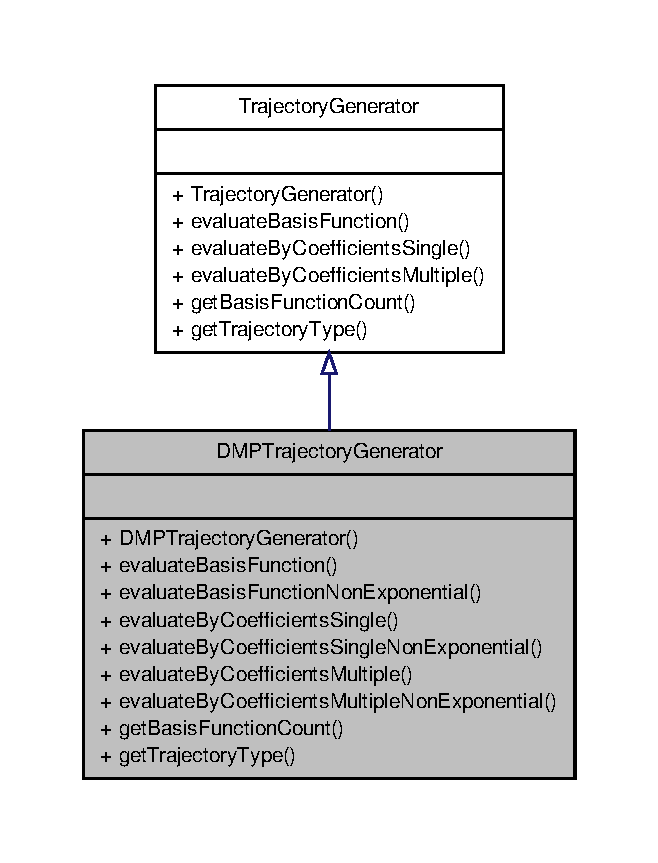
\includegraphics[width=316pt]{classDMPTrajectoryGenerator__inherit__graph}
\end{center}
\end{figure}


\-Collaboration diagram for \-D\-M\-P\-Trajectory\-Generator\-:\nopagebreak
\begin{figure}[H]
\begin{center}
\leavevmode
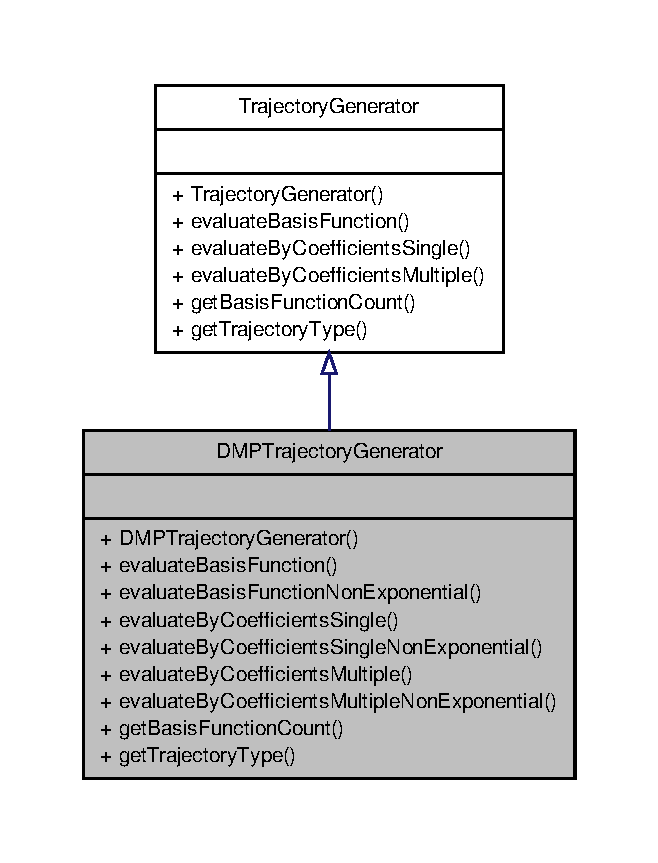
\includegraphics[width=316pt]{classDMPTrajectoryGenerator__coll__graph}
\end{center}
\end{figure}
\subsection*{\-Public \-Member \-Functions}
\begin{DoxyCompactItemize}
\item 
\hyperlink{classDMPTrajectoryGenerator_afb19649fe4c57dae73a44246517f0d93}{\-D\-M\-P\-Trajectory\-Generator} (dmp\-\_\-base\-\_\-set base\-Def, double ax, double tau)
\begin{DoxyCompactList}\small\item\em constructor \end{DoxyCompactList}\item 
double \hyperlink{classDMPTrajectoryGenerator_a992493451729424e9c6420f112614b25}{evaluate\-Basis\-Function} (double x, int fun)
\begin{DoxyCompactList}\small\item\em evaluates the value of a single basis function \end{DoxyCompactList}\item 
double \hyperlink{classDMPTrajectoryGenerator_a7ea77e621ceaf48757bc55fc9b3e4eaf}{evaluate\-Basis\-Function\-Non\-Exponential} (double x, int fun)
\begin{DoxyCompactList}\small\item\em computes the basis function value by setting x = e$^\wedge$(-\/ax / tau $\ast$ x) \end{DoxyCompactList}\item 
double \hyperlink{classDMPTrajectoryGenerator_ad5937ddc13203ab6b11e5366a0c9b57d}{evaluate\-By\-Coefficients\-Single} (double x, vec coeff)
\begin{DoxyCompactList}\small\item\em evaluates the linear combination of basis functions by defining the coefficients for a single value x \end{DoxyCompactList}\item 
double \hyperlink{classDMPTrajectoryGenerator_aa5e6de04ce60232ca1f80c58f8014fe2}{evaluate\-By\-Coefficients\-Single\-Non\-Exponential} (double x, vec coeff)
\begin{DoxyCompactList}\small\item\em computes the linear combination of basis functions values by setting x = e$^\wedge$(-\/ax / tau $\ast$ x) \end{DoxyCompactList}\item 
vec \hyperlink{classDMPTrajectoryGenerator_abd9752e2ff28ad3f2e92b333d3d59d9b}{evaluate\-By\-Coefficients\-Multiple} (vec x, int sample\-Count, vec coeff)
\begin{DoxyCompactList}\small\item\em performs the same as evaluate\-By\-Coefficients\-Single, but for multiple values of x \end{DoxyCompactList}\item 
vec \hyperlink{classDMPTrajectoryGenerator_a1e926f56eea491b06303b682c16aa0bd}{evaluate\-By\-Coefficients\-Multiple\-Non\-Exponential} (vec x, int sample\-Count, vec coeff)
\begin{DoxyCompactList}\small\item\em computes the linear combination of basis functions values for multiple positions by setting x = e$^\wedge$(-\/ax / tau $\ast$ x) \end{DoxyCompactList}\item 
int \hyperlink{classDMPTrajectoryGenerator_add61de058ac17ce262236066a22bb2d6}{get\-Basis\-Function\-Count} ()
\begin{DoxyCompactList}\small\item\em returns the number of basis functions \end{DoxyCompactList}\item 
string \hyperlink{classDMPTrajectoryGenerator_a69dffc9351054b936ddb9285b4065b3d}{get\-Trajectory\-Type} ()
\begin{DoxyCompactList}\small\item\em returns the name of the basis function system as a string \end{DoxyCompactList}\end{DoxyCompactItemize}


\subsection{\-Detailed \-Description}
\-This class provides the basis functions for learning dynamic movement primitives with linear regression (see papers on dmps) 

\subsection{\-Constructor \& \-Destructor \-Documentation}
\hypertarget{classDMPTrajectoryGenerator_afb19649fe4c57dae73a44246517f0d93}{\index{\-D\-M\-P\-Trajectory\-Generator@{\-D\-M\-P\-Trajectory\-Generator}!\-D\-M\-P\-Trajectory\-Generator@{\-D\-M\-P\-Trajectory\-Generator}}
\index{\-D\-M\-P\-Trajectory\-Generator@{\-D\-M\-P\-Trajectory\-Generator}!DMPTrajectoryGenerator@{\-D\-M\-P\-Trajectory\-Generator}}
\subsubsection[{\-D\-M\-P\-Trajectory\-Generator}]{\setlength{\rightskip}{0pt plus 5cm}{\bf \-D\-M\-P\-Trajectory\-Generator\-::\-D\-M\-P\-Trajectory\-Generator} (
\begin{DoxyParamCaption}
\item[{dmp\-\_\-base\-\_\-set}]{base\-Def, }
\item[{double}]{ax, }
\item[{double}]{tau}
\end{DoxyParamCaption}
)}}\label{classDMPTrajectoryGenerator_afb19649fe4c57dae73a44246517f0d93}

\begin{DoxyParams}{\-Parameters}
{\em base\-Def} & defines the basis functions by setting the means and variances of the \-Gaussian basis functions \\
\hline
{\em ax} & dmp constant \\
\hline
{\em tau} & dmp time constant \\
\hline
\end{DoxyParams}


\subsection{\-Member \-Function \-Documentation}
\hypertarget{classDMPTrajectoryGenerator_a992493451729424e9c6420f112614b25}{\index{\-D\-M\-P\-Trajectory\-Generator@{\-D\-M\-P\-Trajectory\-Generator}!evaluate\-Basis\-Function@{evaluate\-Basis\-Function}}
\index{evaluate\-Basis\-Function@{evaluate\-Basis\-Function}!DMPTrajectoryGenerator@{\-D\-M\-P\-Trajectory\-Generator}}
\subsubsection[{evaluate\-Basis\-Function}]{\setlength{\rightskip}{0pt plus 5cm}double {\bf \-D\-M\-P\-Trajectory\-Generator\-::evaluate\-Basis\-Function} (
\begin{DoxyParamCaption}
\item[{double}]{x, }
\item[{int}]{fun}
\end{DoxyParamCaption}
)\hspace{0.3cm}{\ttfamily  \mbox{[}virtual\mbox{]}}}}\label{classDMPTrajectoryGenerator_a992493451729424e9c6420f112614b25}

\begin{DoxyParams}{\-Parameters}
{\em x} & value, where the basis function should be evaluated \\
\hline
{\em fun} & basis function index that specifies the basis function \\
\hline
\end{DoxyParams}


\-Implements \hyperlink{classTrajectoryGenerator_a2f2305b2cb435b0fa7685937516022e1}{\-Trajectory\-Generator}.

\hypertarget{classDMPTrajectoryGenerator_a7ea77e621ceaf48757bc55fc9b3e4eaf}{\index{\-D\-M\-P\-Trajectory\-Generator@{\-D\-M\-P\-Trajectory\-Generator}!evaluate\-Basis\-Function\-Non\-Exponential@{evaluate\-Basis\-Function\-Non\-Exponential}}
\index{evaluate\-Basis\-Function\-Non\-Exponential@{evaluate\-Basis\-Function\-Non\-Exponential}!DMPTrajectoryGenerator@{\-D\-M\-P\-Trajectory\-Generator}}
\subsubsection[{evaluate\-Basis\-Function\-Non\-Exponential}]{\setlength{\rightskip}{0pt plus 5cm}double {\bf \-D\-M\-P\-Trajectory\-Generator\-::evaluate\-Basis\-Function\-Non\-Exponential} (
\begin{DoxyParamCaption}
\item[{double}]{x, }
\item[{int}]{fun}
\end{DoxyParamCaption}
)}}\label{classDMPTrajectoryGenerator_a7ea77e621ceaf48757bc55fc9b3e4eaf}

\begin{DoxyParams}{\-Parameters}
{\em x} & position to evaluate \\
\hline
{\em fun} & basis function index \\
\hline
\end{DoxyParams}
\hypertarget{classDMPTrajectoryGenerator_abd9752e2ff28ad3f2e92b333d3d59d9b}{\index{\-D\-M\-P\-Trajectory\-Generator@{\-D\-M\-P\-Trajectory\-Generator}!evaluate\-By\-Coefficients\-Multiple@{evaluate\-By\-Coefficients\-Multiple}}
\index{evaluate\-By\-Coefficients\-Multiple@{evaluate\-By\-Coefficients\-Multiple}!DMPTrajectoryGenerator@{\-D\-M\-P\-Trajectory\-Generator}}
\subsubsection[{evaluate\-By\-Coefficients\-Multiple}]{\setlength{\rightskip}{0pt plus 5cm}vec {\bf \-D\-M\-P\-Trajectory\-Generator\-::evaluate\-By\-Coefficients\-Multiple} (
\begin{DoxyParamCaption}
\item[{vec}]{x, }
\item[{int}]{sample\-Count, }
\item[{vec}]{coeff}
\end{DoxyParamCaption}
)\hspace{0.3cm}{\ttfamily  \mbox{[}virtual\mbox{]}}}}\label{classDMPTrajectoryGenerator_abd9752e2ff28ad3f2e92b333d3d59d9b}

\begin{DoxyParams}{\-Parameters}
{\em x} & vector of evaluation points \\
\hline
{\em sample\-Count} & size of vector x \\
\hline
{\em coeff} & coefficients that have to be used for computing the linear combination \\
\hline
\end{DoxyParams}


\-Implements \hyperlink{classTrajectoryGenerator_a015de9be72b70ce71675069f4b3361c2}{\-Trajectory\-Generator}.

\hypertarget{classDMPTrajectoryGenerator_a1e926f56eea491b06303b682c16aa0bd}{\index{\-D\-M\-P\-Trajectory\-Generator@{\-D\-M\-P\-Trajectory\-Generator}!evaluate\-By\-Coefficients\-Multiple\-Non\-Exponential@{evaluate\-By\-Coefficients\-Multiple\-Non\-Exponential}}
\index{evaluate\-By\-Coefficients\-Multiple\-Non\-Exponential@{evaluate\-By\-Coefficients\-Multiple\-Non\-Exponential}!DMPTrajectoryGenerator@{\-D\-M\-P\-Trajectory\-Generator}}
\subsubsection[{evaluate\-By\-Coefficients\-Multiple\-Non\-Exponential}]{\setlength{\rightskip}{0pt plus 5cm}vec {\bf \-D\-M\-P\-Trajectory\-Generator\-::evaluate\-By\-Coefficients\-Multiple\-Non\-Exponential} (
\begin{DoxyParamCaption}
\item[{vec}]{x, }
\item[{int}]{sample\-Count, }
\item[{vec}]{coeff}
\end{DoxyParamCaption}
)}}\label{classDMPTrajectoryGenerator_a1e926f56eea491b06303b682c16aa0bd}

\begin{DoxyParams}{\-Parameters}
{\em x} & vector of positions to evaluate \\
\hline
{\em sample\-Count} & size of vector x \\
\hline
{\em coeff} & vector of basis function coefficients \\
\hline
\end{DoxyParams}
\hypertarget{classDMPTrajectoryGenerator_ad5937ddc13203ab6b11e5366a0c9b57d}{\index{\-D\-M\-P\-Trajectory\-Generator@{\-D\-M\-P\-Trajectory\-Generator}!evaluate\-By\-Coefficients\-Single@{evaluate\-By\-Coefficients\-Single}}
\index{evaluate\-By\-Coefficients\-Single@{evaluate\-By\-Coefficients\-Single}!DMPTrajectoryGenerator@{\-D\-M\-P\-Trajectory\-Generator}}
\subsubsection[{evaluate\-By\-Coefficients\-Single}]{\setlength{\rightskip}{0pt plus 5cm}double {\bf \-D\-M\-P\-Trajectory\-Generator\-::evaluate\-By\-Coefficients\-Single} (
\begin{DoxyParamCaption}
\item[{double}]{x, }
\item[{vec}]{coeff}
\end{DoxyParamCaption}
)\hspace{0.3cm}{\ttfamily  \mbox{[}virtual\mbox{]}}}}\label{classDMPTrajectoryGenerator_ad5937ddc13203ab6b11e5366a0c9b57d}

\begin{DoxyParams}{\-Parameters}
{\em x} & value, where the basis functions should be evaluated \\
\hline
{\em coeff} & coefficients that have to be used for computing the linear combination \\
\hline
\end{DoxyParams}


\-Implements \hyperlink{classTrajectoryGenerator_adcc7ede9c713112796a9fc9f1bf4fec2}{\-Trajectory\-Generator}.

\hypertarget{classDMPTrajectoryGenerator_aa5e6de04ce60232ca1f80c58f8014fe2}{\index{\-D\-M\-P\-Trajectory\-Generator@{\-D\-M\-P\-Trajectory\-Generator}!evaluate\-By\-Coefficients\-Single\-Non\-Exponential@{evaluate\-By\-Coefficients\-Single\-Non\-Exponential}}
\index{evaluate\-By\-Coefficients\-Single\-Non\-Exponential@{evaluate\-By\-Coefficients\-Single\-Non\-Exponential}!DMPTrajectoryGenerator@{\-D\-M\-P\-Trajectory\-Generator}}
\subsubsection[{evaluate\-By\-Coefficients\-Single\-Non\-Exponential}]{\setlength{\rightskip}{0pt plus 5cm}double {\bf \-D\-M\-P\-Trajectory\-Generator\-::evaluate\-By\-Coefficients\-Single\-Non\-Exponential} (
\begin{DoxyParamCaption}
\item[{double}]{x, }
\item[{vec}]{coeff}
\end{DoxyParamCaption}
)}}\label{classDMPTrajectoryGenerator_aa5e6de04ce60232ca1f80c58f8014fe2}

\begin{DoxyParams}{\-Parameters}
{\em x} & position to evaluate \\
\hline
{\em coeff} & vector of basis function coefficients \\
\hline
\end{DoxyParams}
\hypertarget{classDMPTrajectoryGenerator_add61de058ac17ce262236066a22bb2d6}{\index{\-D\-M\-P\-Trajectory\-Generator@{\-D\-M\-P\-Trajectory\-Generator}!get\-Basis\-Function\-Count@{get\-Basis\-Function\-Count}}
\index{get\-Basis\-Function\-Count@{get\-Basis\-Function\-Count}!DMPTrajectoryGenerator@{\-D\-M\-P\-Trajectory\-Generator}}
\subsubsection[{get\-Basis\-Function\-Count}]{\setlength{\rightskip}{0pt plus 5cm}int {\bf \-D\-M\-P\-Trajectory\-Generator\-::get\-Basis\-Function\-Count} (
\begin{DoxyParamCaption}
{}
\end{DoxyParamCaption}
)\hspace{0.3cm}{\ttfamily  \mbox{[}virtual\mbox{]}}}}\label{classDMPTrajectoryGenerator_add61de058ac17ce262236066a22bb2d6}


\-Implements \hyperlink{classTrajectoryGenerator_a8d3c339d0c8488873074c8bce918afae}{\-Trajectory\-Generator}.

\hypertarget{classDMPTrajectoryGenerator_a69dffc9351054b936ddb9285b4065b3d}{\index{\-D\-M\-P\-Trajectory\-Generator@{\-D\-M\-P\-Trajectory\-Generator}!get\-Trajectory\-Type@{get\-Trajectory\-Type}}
\index{get\-Trajectory\-Type@{get\-Trajectory\-Type}!DMPTrajectoryGenerator@{\-D\-M\-P\-Trajectory\-Generator}}
\subsubsection[{get\-Trajectory\-Type}]{\setlength{\rightskip}{0pt plus 5cm}string {\bf \-D\-M\-P\-Trajectory\-Generator\-::get\-Trajectory\-Type} (
\begin{DoxyParamCaption}
{}
\end{DoxyParamCaption}
)\hspace{0.3cm}{\ttfamily  \mbox{[}virtual\mbox{]}}}}\label{classDMPTrajectoryGenerator_a69dffc9351054b936ddb9285b4065b3d}


\-Implements \hyperlink{classTrajectoryGenerator_a14e3b583fcee58d393360ef0eb0fb71c}{\-Trajectory\-Generator}.



\-The documentation for this class was generated from the following files\-:\begin{DoxyCompactItemize}
\item 
/home/shangl/data/data\-\_\-synched/studium/informatik/master/master\-\_\-thesis/kukadu\-\_\-framework/thesis/src/trajectory/\hyperlink{DMPTrajectoryGenerator_8h}{\-D\-M\-P\-Trajectory\-Generator.\-h}\item 
/home/shangl/data/data\-\_\-synched/studium/informatik/master/master\-\_\-thesis/kukadu\-\_\-framework/thesis/src/trajectory/\hyperlink{DMPTrajectoryGenerator_8cpp}{\-D\-M\-P\-Trajectory\-Generator.\-cpp}\end{DoxyCompactItemize}

\hypertarget{classGaussianKernel}{\section{\-Gaussian\-Kernel \-Class \-Reference}
\label{classGaussianKernel}\index{\-Gaussian\-Kernel@{\-Gaussian\-Kernel}}
}


\-Implements a \-Gaussian kernel according to the \hyperlink{classGenericKernel}{\-Generic\-Kernel} specifiction.  




{\ttfamily \#include $<$\-Gaussian\-Kernel.\-h$>$}



\-Inheritance diagram for \-Gaussian\-Kernel\-:\nopagebreak
\begin{figure}[H]
\begin{center}
\leavevmode
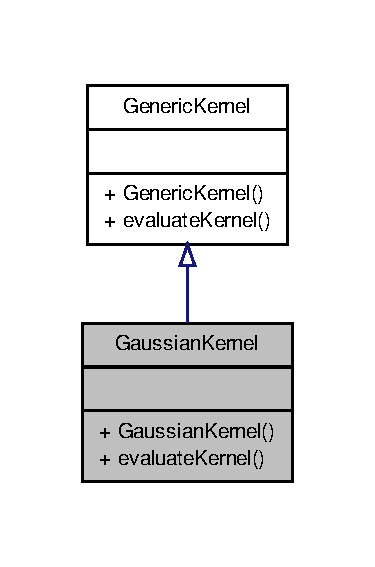
\includegraphics[width=180pt]{classGaussianKernel__inherit__graph}
\end{center}
\end{figure}


\-Collaboration diagram for \-Gaussian\-Kernel\-:\nopagebreak
\begin{figure}[H]
\begin{center}
\leavevmode
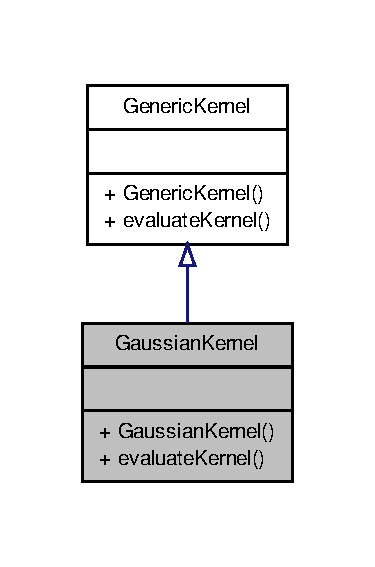
\includegraphics[width=180pt]{classGaussianKernel__coll__graph}
\end{center}
\end{figure}
\subsection*{\-Public \-Member \-Functions}
\begin{DoxyCompactItemize}
\item 
\hyperlink{classGaussianKernel_a8043efa2c1dba7d30e0f597e20fb1d83}{\-Gaussian\-Kernel} (double theta0, double theta1)
\begin{DoxyCompactList}\small\item\em constructor \end{DoxyCompactList}\item 
double \hyperlink{classGaussianKernel_a11e2ca51c88c8167b86c571187995d47}{evaluate\-Kernel} (vec q1, vec q2, void $\ast$kernel\-Param)
\begin{DoxyCompactList}\small\item\em computes kernel values with given vectors q1 and q2 and passes a not further specified kernel parameter that can be used by the kernel implementation \end{DoxyCompactList}\end{DoxyCompactItemize}


\subsection{\-Detailed \-Description}
\-This class implements a \-Gaussian kernel given by the function \-K(u) = theta0 e$^\wedge$(-\/ theta1 /2 u$^\wedge$2) 

\subsection{\-Constructor \& \-Destructor \-Documentation}
\hypertarget{classGaussianKernel_a8043efa2c1dba7d30e0f597e20fb1d83}{\index{\-Gaussian\-Kernel@{\-Gaussian\-Kernel}!\-Gaussian\-Kernel@{\-Gaussian\-Kernel}}
\index{\-Gaussian\-Kernel@{\-Gaussian\-Kernel}!GaussianKernel@{\-Gaussian\-Kernel}}
\subsubsection[{\-Gaussian\-Kernel}]{\setlength{\rightskip}{0pt plus 5cm}{\bf \-Gaussian\-Kernel\-::\-Gaussian\-Kernel} (
\begin{DoxyParamCaption}
\item[{double}]{theta0, }
\item[{double}]{theta1}
\end{DoxyParamCaption}
)}}\label{classGaussianKernel_a8043efa2c1dba7d30e0f597e20fb1d83}

\begin{DoxyParams}{\-Parameters}
{\em theta0} & paremeter theta0 of the kernel according to the given kernel function \\
\hline
{\em theta1} & paremeter theta1 of the kernel according to the given kernel function \\
\hline
\end{DoxyParams}


\subsection{\-Member \-Function \-Documentation}
\hypertarget{classGaussianKernel_a11e2ca51c88c8167b86c571187995d47}{\index{\-Gaussian\-Kernel@{\-Gaussian\-Kernel}!evaluate\-Kernel@{evaluate\-Kernel}}
\index{evaluate\-Kernel@{evaluate\-Kernel}!GaussianKernel@{\-Gaussian\-Kernel}}
\subsubsection[{evaluate\-Kernel}]{\setlength{\rightskip}{0pt plus 5cm}double {\bf \-Gaussian\-Kernel\-::evaluate\-Kernel} (
\begin{DoxyParamCaption}
\item[{vec}]{q1, }
\item[{vec}]{q2, }
\item[{void $\ast$}]{kernel\-Param}
\end{DoxyParamCaption}
)\hspace{0.3cm}{\ttfamily  \mbox{[}virtual\mbox{]}}}}\label{classGaussianKernel_a11e2ca51c88c8167b86c571187995d47}

\begin{DoxyParams}{\-Parameters}
{\em q1} & vector q1 with \-K = \-K(d(q1, q2)) \\
\hline
{\em q2} & vector q2 with \-K = \-K(d(q1, q2)) \\
\hline
{\em kernel\-Param} & arbitrary kernel parameter \\
\hline
\end{DoxyParams}


\-Implements \hyperlink{classGenericKernel_a5b3ef309f47d56cfcb12d02bf0f0b5c7}{\-Generic\-Kernel}.



\-The documentation for this class was generated from the following files\-:\begin{DoxyCompactItemize}
\item 
/home/shangl/data/data\-\_\-synched/studium/informatik/master/master\-\_\-thesis/kukadu\-\_\-framework/thesis/src/learning/\hyperlink{GaussianKernel_8h}{\-Gaussian\-Kernel.\-h}\item 
/home/shangl/data/data\-\_\-synched/studium/informatik/master/master\-\_\-thesis/kukadu\-\_\-framework/thesis/src/learning/\hyperlink{GaussianKernel_8cpp}{\-Gaussian\-Kernel.\-cpp}\end{DoxyCompactItemize}

\hypertarget{classGaussianProcessRegressor}{\section{\-Gaussian\-Process\-Regressor \-Class \-Reference}
\label{classGaussianProcessRegressor}\index{\-Gaussian\-Process\-Regressor@{\-Gaussian\-Process\-Regressor}}
}


\-Implements the \-Gaussian process regression method.  




{\ttfamily \#include $<$\-Gaussian\-Process\-Regressor.\-h$>$}



\-Inheritance diagram for \-Gaussian\-Process\-Regressor\-:\nopagebreak
\begin{figure}[H]
\begin{center}
\leavevmode
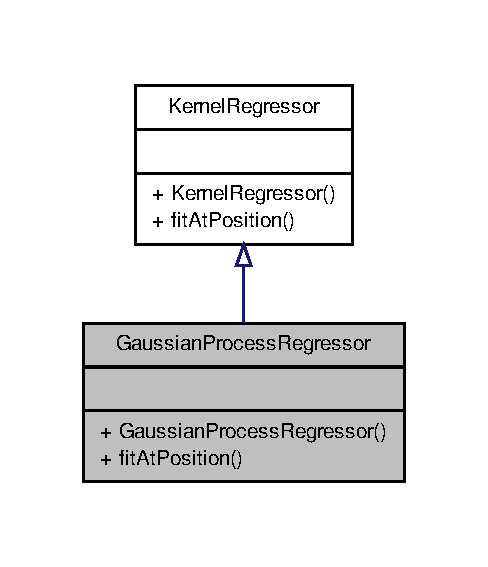
\includegraphics[width=234pt]{classGaussianProcessRegressor__inherit__graph}
\end{center}
\end{figure}


\-Collaboration diagram for \-Gaussian\-Process\-Regressor\-:\nopagebreak
\begin{figure}[H]
\begin{center}
\leavevmode
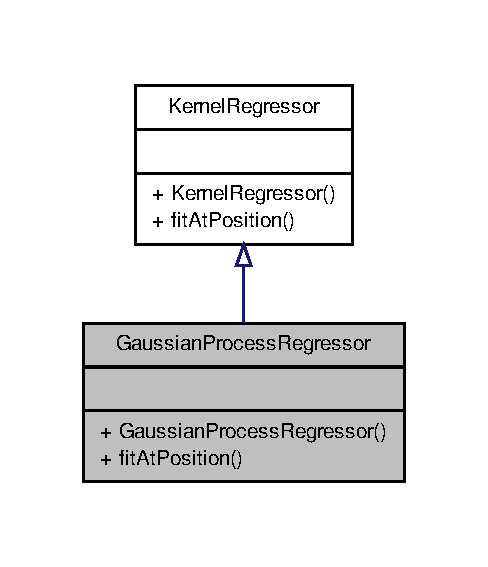
\includegraphics[width=234pt]{classGaussianProcessRegressor__coll__graph}
\end{center}
\end{figure}
\subsection*{\-Public \-Member \-Functions}
\begin{DoxyCompactItemize}
\item 
\hyperlink{classGaussianProcessRegressor_a2465d404e36974f608a735a2c3dd6e9b}{\-Gaussian\-Process\-Regressor} (vector$<$ vec $>$ sample\-Xs, vec sample\-Ts, \hyperlink{classGenericKernel}{\-Generic\-Kernel} $\ast$kernel, double beta)
\begin{DoxyCompactList}\small\item\em constructor, setting all the sample data, the selected kernel and the variance beta \end{DoxyCompactList}\item 
vec \hyperlink{classGaussianProcessRegressor_a9c4ad88ae6cbbc457cbfa17c64e59d1b}{fit\-At\-Position} (vec pos)
\begin{DoxyCompactList}\small\item\em performs the kernel method for predicting the functin value at a given position \end{DoxyCompactList}\end{DoxyCompactItemize}


\subsection{\-Detailed \-Description}
\-This class inherits from the \hyperlink{classKernelRegressor}{\-Kernel\-Regressor} and implements \-Gaussian process regression. 

\subsection{\-Constructor \& \-Destructor \-Documentation}
\hypertarget{classGaussianProcessRegressor_a2465d404e36974f608a735a2c3dd6e9b}{\index{\-Gaussian\-Process\-Regressor@{\-Gaussian\-Process\-Regressor}!\-Gaussian\-Process\-Regressor@{\-Gaussian\-Process\-Regressor}}
\index{\-Gaussian\-Process\-Regressor@{\-Gaussian\-Process\-Regressor}!GaussianProcessRegressor@{\-Gaussian\-Process\-Regressor}}
\subsubsection[{\-Gaussian\-Process\-Regressor}]{\setlength{\rightskip}{0pt plus 5cm}{\bf \-Gaussian\-Process\-Regressor\-::\-Gaussian\-Process\-Regressor} (
\begin{DoxyParamCaption}
\item[{vector$<$ vec $>$}]{sample\-Xs, }
\item[{vec}]{sample\-Ts, }
\item[{{\bf \-Generic\-Kernel} $\ast$}]{kernel, }
\item[{double}]{beta}
\end{DoxyParamCaption}
)}}\label{classGaussianProcessRegressor_a2465d404e36974f608a735a2c3dd6e9b}

\begin{DoxyParams}{\-Parameters}
{\em sample\-Xs} & vector of samples (x-\/axis) \\
\hline
{\em sample\-Ts} & vector of samples (y-\/axis) \\
\hline
{\em kernel} & the selected kernel implementation \\
\hline
{\em beta} & the assumed sample variance \\
\hline
\end{DoxyParams}


\subsection{\-Member \-Function \-Documentation}
\hypertarget{classGaussianProcessRegressor_a9c4ad88ae6cbbc457cbfa17c64e59d1b}{\index{\-Gaussian\-Process\-Regressor@{\-Gaussian\-Process\-Regressor}!fit\-At\-Position@{fit\-At\-Position}}
\index{fit\-At\-Position@{fit\-At\-Position}!GaussianProcessRegressor@{\-Gaussian\-Process\-Regressor}}
\subsubsection[{fit\-At\-Position}]{\setlength{\rightskip}{0pt plus 5cm}vec {\bf \-Gaussian\-Process\-Regressor\-::fit\-At\-Position} (
\begin{DoxyParamCaption}
\item[{vec}]{pos}
\end{DoxyParamCaption}
)\hspace{0.3cm}{\ttfamily  \mbox{[}virtual\mbox{]}}}}\label{classGaussianProcessRegressor_a9c4ad88ae6cbbc457cbfa17c64e59d1b}

\begin{DoxyParams}{\-Parameters}
{\em pos} & vector defining the required position \\
\hline
\end{DoxyParams}


\-Implements \hyperlink{classKernelRegressor_a65529e1d764f9abf0498c93a35ac3f16}{\-Kernel\-Regressor}.



\-The documentation for this class was generated from the following files\-:\begin{DoxyCompactItemize}
\item 
/home/shangl/data/data\-\_\-synched/studium/informatik/master/master\-\_\-thesis/kukadu\-\_\-framework/thesis/src/learning/\hyperlink{GaussianProcessRegressor_8h}{\-Gaussian\-Process\-Regressor.\-h}\item 
/home/shangl/data/data\-\_\-synched/studium/informatik/master/master\-\_\-thesis/kukadu\-\_\-framework/thesis/src/learning/\hyperlink{GaussianProcessRegressor_8cpp}{\-Gaussian\-Process\-Regressor.\-cpp}\end{DoxyCompactItemize}

\hypertarget{classGenDMPReinforcer}{\section{\-Gen\-D\-M\-P\-Reinforcer \-Class \-Reference}
\label{classGenDMPReinforcer}\index{\-Gen\-D\-M\-P\-Reinforcer@{\-Gen\-D\-M\-P\-Reinforcer}}
}


\-The \hyperlink{classGenDMPReinforcer}{\-Gen\-D\-M\-P\-Reinforcer} completes the \hyperlink{classDMPReinforcer}{\-D\-M\-P\-Reinforcer} implementation by reusing the \hyperlink{classDMPGeneralizer}{\-D\-M\-P\-Generalizer} functionality.  




{\ttfamily \#include $<$\-Gen\-D\-M\-P\-Reinforcer.\-h$>$}



\-Inheritance diagram for \-Gen\-D\-M\-P\-Reinforcer\-:
\nopagebreak
\begin{figure}[H]
\begin{center}
\leavevmode
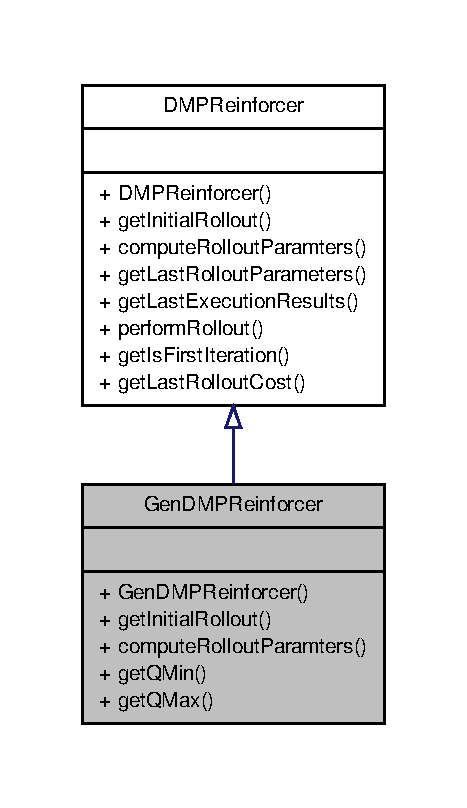
\includegraphics[width=224pt]{classGenDMPReinforcer__inherit__graph}
\end{center}
\end{figure}


\-Collaboration diagram for \-Gen\-D\-M\-P\-Reinforcer\-:
\nopagebreak
\begin{figure}[H]
\begin{center}
\leavevmode
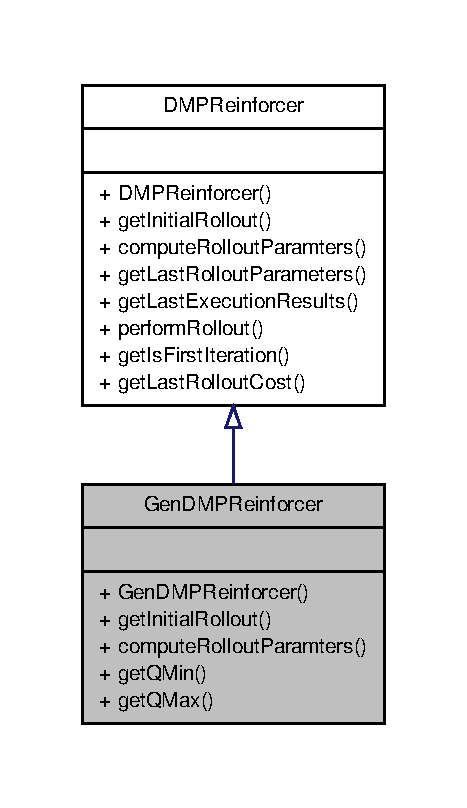
\includegraphics[width=224pt]{classGenDMPReinforcer__coll__graph}
\end{center}
\end{figure}
\subsection*{\-Public \-Member \-Functions}
\begin{DoxyCompactItemize}
\item 
\hyperlink{classGenDMPReinforcer_ad57993f556bff5c44af1f74b2804761b}{\-Gen\-D\-M\-P\-Reinforcer} (vec initial\-Query\-Point, \hyperlink{classCostComputer}{\-Cost\-Computer} $\ast$cost, \hyperlink{classDMPGeneralizer}{\-D\-M\-P\-Generalizer} $\ast$dmp\-Gen, \hyperlink{classGenericKernel}{\-Generic\-Kernel} $\ast$trajectory\-Kernel, \hyperlink{classGenericKernel}{\-Generic\-Kernel} $\ast$parameter\-Kernel, \hyperlink{classControlQueue}{\-Control\-Queue} $\ast$movement\-Queue, double ac, double dmp\-Step\-Size, double tol\-Abs\-Err, double tol\-Rel\-Err)
\begin{DoxyCompactList}\small\item\em constructor \end{DoxyCompactList}\item 
t\-\_\-learned\-\_\-dmp \hyperlink{classGenDMPReinforcer_adf7e9353b54e429649fb5dd5dd17c28e}{get\-Initial\-Rollout} ()
\begin{DoxyCompactList}\small\item\em returns the first rollout of the reinforcement learning algorithm \end{DoxyCompactList}\item 
t\-\_\-learned\-\_\-dmp \hyperlink{classGenDMPReinforcer_aace5aaa5519a64a33f05b0fd95ac0b6e}{compute\-Rollout\-Paramters} ()
\begin{DoxyCompactList}\small\item\em computes the dmp parameters for the next rollout \end{DoxyCompactList}\item 
double \hyperlink{classGenDMPReinforcer_aaeb0d7711cfc43d52b35a8ba8e0698b9}{get\-Q\-Min} ()
\begin{DoxyCompactList}\small\item\em returns maximum query point \end{DoxyCompactList}\item 
double \hyperlink{classGenDMPReinforcer_a70498092175c9c6f81ce379323263ace}{get\-Q\-Max} ()
\begin{DoxyCompactList}\small\item\em returns minimum query point \end{DoxyCompactList}\end{DoxyCompactItemize}


\subsection{\-Detailed \-Description}
\-This class computes the next rollout by working in the low dimensional query space of the method implemented by the \hyperlink{classDMPGeneralizer}{\-D\-M\-P\-Generalizer}. \-Therefore, the precondition of this method are similar trajectories for nearby query points. \-This implementation can only handle one dimensional query points. 

\subsection{\-Constructor \& \-Destructor \-Documentation}
\hypertarget{classGenDMPReinforcer_ad57993f556bff5c44af1f74b2804761b}{\index{\-Gen\-D\-M\-P\-Reinforcer@{\-Gen\-D\-M\-P\-Reinforcer}!\-Gen\-D\-M\-P\-Reinforcer@{\-Gen\-D\-M\-P\-Reinforcer}}
\index{\-Gen\-D\-M\-P\-Reinforcer@{\-Gen\-D\-M\-P\-Reinforcer}!GenDMPReinforcer@{\-Gen\-D\-M\-P\-Reinforcer}}
\subsubsection[{\-Gen\-D\-M\-P\-Reinforcer}]{\setlength{\rightskip}{0pt plus 5cm}{\bf \-Gen\-D\-M\-P\-Reinforcer\-::\-Gen\-D\-M\-P\-Reinforcer} (
\begin{DoxyParamCaption}
\item[{vec}]{initial\-Query\-Point, }
\item[{{\bf \-Cost\-Computer} $\ast$}]{cost, }
\item[{{\bf \-D\-M\-P\-Generalizer} $\ast$}]{dmp\-Gen, }
\item[{{\bf \-Generic\-Kernel} $\ast$}]{trajectory\-Kernel, }
\item[{{\bf \-Generic\-Kernel} $\ast$}]{parameter\-Kernel, }
\item[{{\bf \-Control\-Queue} $\ast$}]{movement\-Queue, }
\item[{double}]{ac, }
\item[{double}]{dmp\-Step\-Size, }
\item[{double}]{tol\-Abs\-Err, }
\item[{double}]{tol\-Rel\-Err}
\end{DoxyParamCaption}
)}}\label{classGenDMPReinforcer_ad57993f556bff5c44af1f74b2804761b}

\begin{DoxyParams}{\-Parameters}
{\em initial\-Query\-Point} & desired query point for which reinforcement learning should be applied \\
\hline
{\em cost} & \hyperlink{classCostComputer}{\-Cost\-Computer} implementation \\
\hline
{\em dmp\-Gen} & \hyperlink{classDMPGeneralizer}{\-D\-M\-P\-Generalizer} instance \\
\hline
{\em trajectory\-Kernel} & generalization kernel (see \hyperlink{classDMPGeneralizer}{\-D\-M\-P\-Generalizer} documentation) \\
\hline
{\em parameter\-Kernel} & generalization kernel (see \hyperlink{classDMPGeneralizer}{\-D\-M\-P\-Generalizer} documentation) \\
\hline
{\em movement\-Queue} & control queue for robot execution \\
\hline
{\em ac} & phase stopping parameter \\
\hline
{\em dmp\-Step\-Size} & step size for dmp execution \\
\hline
{\em tol\-Abs\-Err} & absolute tolerated error for numerical approximation \\
\hline
{\em tol\-Rel\-Err} & relative tolerated error for numerical approximation \\
\hline
\end{DoxyParams}


\subsection{\-Member \-Function \-Documentation}
\hypertarget{classGenDMPReinforcer_aace5aaa5519a64a33f05b0fd95ac0b6e}{\index{\-Gen\-D\-M\-P\-Reinforcer@{\-Gen\-D\-M\-P\-Reinforcer}!compute\-Rollout\-Paramters@{compute\-Rollout\-Paramters}}
\index{compute\-Rollout\-Paramters@{compute\-Rollout\-Paramters}!GenDMPReinforcer@{\-Gen\-D\-M\-P\-Reinforcer}}
\subsubsection[{compute\-Rollout\-Paramters}]{\setlength{\rightskip}{0pt plus 5cm}t\-\_\-learned\-\_\-dmp {\bf \-Gen\-D\-M\-P\-Reinforcer\-::compute\-Rollout\-Paramters} (
\begin{DoxyParamCaption}
{}
\end{DoxyParamCaption}
)\hspace{0.3cm}{\ttfamily  \mbox{[}virtual\mbox{]}}}}\label{classGenDMPReinforcer_aace5aaa5519a64a33f05b0fd95ac0b6e}


\-Implements \hyperlink{classDMPReinforcer_a0c82b35d96fe07663187b8befd5c1042}{\-D\-M\-P\-Reinforcer}.

\hypertarget{classGenDMPReinforcer_adf7e9353b54e429649fb5dd5dd17c28e}{\index{\-Gen\-D\-M\-P\-Reinforcer@{\-Gen\-D\-M\-P\-Reinforcer}!get\-Initial\-Rollout@{get\-Initial\-Rollout}}
\index{get\-Initial\-Rollout@{get\-Initial\-Rollout}!GenDMPReinforcer@{\-Gen\-D\-M\-P\-Reinforcer}}
\subsubsection[{get\-Initial\-Rollout}]{\setlength{\rightskip}{0pt plus 5cm}t\-\_\-learned\-\_\-dmp {\bf \-Gen\-D\-M\-P\-Reinforcer\-::get\-Initial\-Rollout} (
\begin{DoxyParamCaption}
{}
\end{DoxyParamCaption}
)\hspace{0.3cm}{\ttfamily  \mbox{[}virtual\mbox{]}}}}\label{classGenDMPReinforcer_adf7e9353b54e429649fb5dd5dd17c28e}


\-Implements \hyperlink{classDMPReinforcer_aa9459e4d8a500cc6851e19a804680db7}{\-D\-M\-P\-Reinforcer}.

\hypertarget{classGenDMPReinforcer_a70498092175c9c6f81ce379323263ace}{\index{\-Gen\-D\-M\-P\-Reinforcer@{\-Gen\-D\-M\-P\-Reinforcer}!get\-Q\-Max@{get\-Q\-Max}}
\index{get\-Q\-Max@{get\-Q\-Max}!GenDMPReinforcer@{\-Gen\-D\-M\-P\-Reinforcer}}
\subsubsection[{get\-Q\-Max}]{\setlength{\rightskip}{0pt plus 5cm}double {\bf \-Gen\-D\-M\-P\-Reinforcer\-::get\-Q\-Max} (
\begin{DoxyParamCaption}
{}
\end{DoxyParamCaption}
)}}\label{classGenDMPReinforcer_a70498092175c9c6f81ce379323263ace}
\hypertarget{classGenDMPReinforcer_aaeb0d7711cfc43d52b35a8ba8e0698b9}{\index{\-Gen\-D\-M\-P\-Reinforcer@{\-Gen\-D\-M\-P\-Reinforcer}!get\-Q\-Min@{get\-Q\-Min}}
\index{get\-Q\-Min@{get\-Q\-Min}!GenDMPReinforcer@{\-Gen\-D\-M\-P\-Reinforcer}}
\subsubsection[{get\-Q\-Min}]{\setlength{\rightskip}{0pt plus 5cm}double {\bf \-Gen\-D\-M\-P\-Reinforcer\-::get\-Q\-Min} (
\begin{DoxyParamCaption}
{}
\end{DoxyParamCaption}
)}}\label{classGenDMPReinforcer_aaeb0d7711cfc43d52b35a8ba8e0698b9}


\-The documentation for this class was generated from the following files\-:\begin{DoxyCompactItemize}
\item 
/home/shangl/data/data\-\_\-synched/studium/informatik/master/master\-\_\-thesis/kukadu\-\_\-framework/thesis/src/trajectory/\hyperlink{GenDMPReinforcer_8h}{\-Gen\-D\-M\-P\-Reinforcer.\-h}\item 
/home/shangl/data/data\-\_\-synched/studium/informatik/master/master\-\_\-thesis/kukadu\-\_\-framework/thesis/src/trajectory/\hyperlink{GenDMPReinforcer_8cpp}{\-Gen\-D\-M\-P\-Reinforcer.\-cpp}\end{DoxyCompactItemize}

\hypertarget{classGeneralFitter}{\section{\-General\-Fitter \-Class \-Reference}
\label{classGeneralFitter}\index{\-General\-Fitter@{\-General\-Fitter}}
}


\-Provides the generic part of the linear regression methods.  




{\ttfamily \#include $<$\-General\-Fitter.\-h$>$}

\subsection*{\-Public \-Member \-Functions}
\begin{DoxyCompactItemize}
\item 
\hyperlink{classGeneralFitter_a4177255144dd28bfad12437e558ce932}{\-General\-Fitter} (vec samples\-X, vec samples\-Y, int sample\-Count, \hyperlink{classTrajectoryGenerator}{\-Trajectory\-Generator} $\ast$traj\-Gen)
\begin{DoxyCompactList}\small\item\em constructor \end{DoxyCompactList}\item 
int \hyperlink{classGeneralFitter_aa3fadbccff7bafede20ec9344ee4167a}{get\-Basis\-Function\-Count} ()
\begin{DoxyCompactList}\small\item\em returns the number of basis functions \end{DoxyCompactList}\item 
int \hyperlink{classGeneralFitter_a3d1d98a54d99a1dfd2d86a3b1b0632a8}{get\-Sample\-Count} ()
\begin{DoxyCompactList}\small\item\em returns the number of samples \end{DoxyCompactList}\item 
vec \hyperlink{classGeneralFitter_ad5cb0fdd4dfd2a8ab765f8b4a6a8d4d2}{compute\-Lin\-Fit\-Coefficients} ()
\begin{DoxyCompactList}\small\item\em performs linear regression and returns vector of coefficients corresponding to the basis functions \end{DoxyCompactList}\item 
vec \hyperlink{classGeneralFitter_ad8cb235ca20c654263f0e163436825bb}{compute\-Lin\-Fit\-Coefficients} (mat des\-Mat)
\begin{DoxyCompactList}\small\item\em performs linear regression and returns vector of coefficients corresponding to the basis functions by explicitly taking the design matrix as parameter \end{DoxyCompactList}\item 
mat \hyperlink{classGeneralFitter_a92ddce03f74fc9af37801d011f7f559f}{compute\-Design\-Matrix} ()
\begin{DoxyCompactList}\small\item\em computes design matrix \end{DoxyCompactList}\end{DoxyCompactItemize}


\subsection{\-Detailed \-Description}
\-This class provides implements the generic part of the linear regression method. \-It is independent of the specific choice of basis functions. \-These basis functions are defined via the \hyperlink{classTrajectoryGenerator}{\-Trajectory\-Generator} class. 

\subsection{\-Constructor \& \-Destructor \-Documentation}
\hypertarget{classGeneralFitter_a4177255144dd28bfad12437e558ce932}{\index{\-General\-Fitter@{\-General\-Fitter}!\-General\-Fitter@{\-General\-Fitter}}
\index{\-General\-Fitter@{\-General\-Fitter}!GeneralFitter@{\-General\-Fitter}}
\subsubsection[{\-General\-Fitter}]{\setlength{\rightskip}{0pt plus 5cm}{\bf \-General\-Fitter\-::\-General\-Fitter} (
\begin{DoxyParamCaption}
\item[{vec}]{samples\-X, }
\item[{vec}]{samples\-Y, }
\item[{int}]{sample\-Count, }
\item[{{\bf \-Trajectory\-Generator} $\ast$}]{traj\-Gen}
\end{DoxyParamCaption}
)}}\label{classGeneralFitter_a4177255144dd28bfad12437e558ce932}

\begin{DoxyParams}{\-Parameters}
{\em samples\-X} & vector of samples, where samples\-X specifies the x-\/axis \\
\hline
{\em samples\-Y} & vector of samples, where samples\-Y specifies the y-\/axis \\
\hline
{\em sample\-Count} & number of sample points \\
\hline
{\em traj\-Gen} & \hyperlink{classTrajectoryGenerator}{\-Trajectory\-Generator} instance defining the basis functions \\
\hline
\end{DoxyParams}


\subsection{\-Member \-Function \-Documentation}
\hypertarget{classGeneralFitter_a92ddce03f74fc9af37801d011f7f559f}{\index{\-General\-Fitter@{\-General\-Fitter}!compute\-Design\-Matrix@{compute\-Design\-Matrix}}
\index{compute\-Design\-Matrix@{compute\-Design\-Matrix}!GeneralFitter@{\-General\-Fitter}}
\subsubsection[{compute\-Design\-Matrix}]{\setlength{\rightskip}{0pt plus 5cm}mat {\bf \-General\-Fitter\-::compute\-Design\-Matrix} (
\begin{DoxyParamCaption}
{}
\end{DoxyParamCaption}
)}}\label{classGeneralFitter_a92ddce03f74fc9af37801d011f7f559f}
\hypertarget{classGeneralFitter_ad5cb0fdd4dfd2a8ab765f8b4a6a8d4d2}{\index{\-General\-Fitter@{\-General\-Fitter}!compute\-Lin\-Fit\-Coefficients@{compute\-Lin\-Fit\-Coefficients}}
\index{compute\-Lin\-Fit\-Coefficients@{compute\-Lin\-Fit\-Coefficients}!GeneralFitter@{\-General\-Fitter}}
\subsubsection[{compute\-Lin\-Fit\-Coefficients}]{\setlength{\rightskip}{0pt plus 5cm}vec {\bf \-General\-Fitter\-::compute\-Lin\-Fit\-Coefficients} (
\begin{DoxyParamCaption}
{}
\end{DoxyParamCaption}
)}}\label{classGeneralFitter_ad5cb0fdd4dfd2a8ab765f8b4a6a8d4d2}
\hypertarget{classGeneralFitter_ad8cb235ca20c654263f0e163436825bb}{\index{\-General\-Fitter@{\-General\-Fitter}!compute\-Lin\-Fit\-Coefficients@{compute\-Lin\-Fit\-Coefficients}}
\index{compute\-Lin\-Fit\-Coefficients@{compute\-Lin\-Fit\-Coefficients}!GeneralFitter@{\-General\-Fitter}}
\subsubsection[{compute\-Lin\-Fit\-Coefficients}]{\setlength{\rightskip}{0pt plus 5cm}vec {\bf \-General\-Fitter\-::compute\-Lin\-Fit\-Coefficients} (
\begin{DoxyParamCaption}
\item[{mat}]{des\-Mat}
\end{DoxyParamCaption}
)}}\label{classGeneralFitter_ad8cb235ca20c654263f0e163436825bb}

\begin{DoxyParams}{\-Parameters}
{\em des\-Mat} & design matrix needed for linear regression \\
\hline
\end{DoxyParams}
\hypertarget{classGeneralFitter_aa3fadbccff7bafede20ec9344ee4167a}{\index{\-General\-Fitter@{\-General\-Fitter}!get\-Basis\-Function\-Count@{get\-Basis\-Function\-Count}}
\index{get\-Basis\-Function\-Count@{get\-Basis\-Function\-Count}!GeneralFitter@{\-General\-Fitter}}
\subsubsection[{get\-Basis\-Function\-Count}]{\setlength{\rightskip}{0pt plus 5cm}int {\bf \-General\-Fitter\-::get\-Basis\-Function\-Count} (
\begin{DoxyParamCaption}
{}
\end{DoxyParamCaption}
)}}\label{classGeneralFitter_aa3fadbccff7bafede20ec9344ee4167a}
\hypertarget{classGeneralFitter_a3d1d98a54d99a1dfd2d86a3b1b0632a8}{\index{\-General\-Fitter@{\-General\-Fitter}!get\-Sample\-Count@{get\-Sample\-Count}}
\index{get\-Sample\-Count@{get\-Sample\-Count}!GeneralFitter@{\-General\-Fitter}}
\subsubsection[{get\-Sample\-Count}]{\setlength{\rightskip}{0pt plus 5cm}int {\bf \-General\-Fitter\-::get\-Sample\-Count} (
\begin{DoxyParamCaption}
{}
\end{DoxyParamCaption}
)}}\label{classGeneralFitter_a3d1d98a54d99a1dfd2d86a3b1b0632a8}


\-The documentation for this class was generated from the following files\-:\begin{DoxyCompactItemize}
\item 
/home/shangl/data/data\-\_\-synched/studium/informatik/master/master\-\_\-thesis/kukadu\-\_\-framework/thesis/src/learning/\hyperlink{GeneralFitter_8h}{\-General\-Fitter.\-h}\item 
/home/shangl/data/data\-\_\-synched/studium/informatik/master/master\-\_\-thesis/kukadu\-\_\-framework/thesis/src/learning/\hyperlink{GeneralFitter_8cpp}{\-General\-Fitter.\-cpp}\end{DoxyCompactItemize}

\hypertarget{classGenericHand}{\section{\-Generic\-Hand \-Class \-Reference}
\label{classGenericHand}\index{\-Generic\-Hand@{\-Generic\-Hand}}
}


\-The \hyperlink{classGenericHand}{\-Generic\-Hand} provides a very elementary interface to control robot hands mounted on a robot arm \-This class provides very an interface for the very basic functionalities such as \char`\"{}connect to hand\char`\"{} or \char`\"{}close hand\char`\"{}.  




{\ttfamily \#include $<$\-Generic\-Hand.\-h$>$}



\-Inheritance diagram for \-Generic\-Hand\-:\nopagebreak
\begin{figure}[H]
\begin{center}
\leavevmode
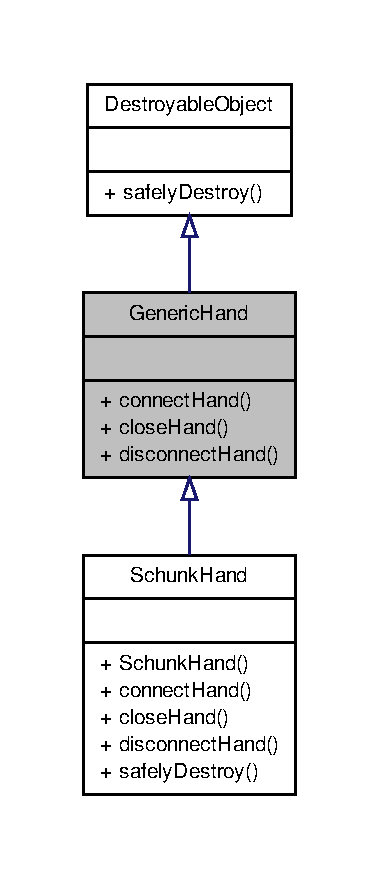
\includegraphics[width=182pt]{classGenericHand__inherit__graph}
\end{center}
\end{figure}


\-Collaboration diagram for \-Generic\-Hand\-:\nopagebreak
\begin{figure}[H]
\begin{center}
\leavevmode
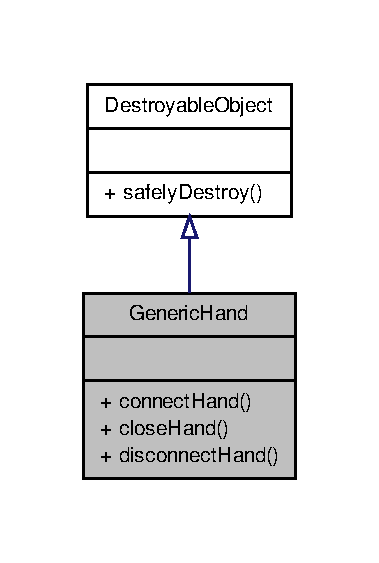
\includegraphics[width=182pt]{classGenericHand__coll__graph}
\end{center}
\end{figure}
\subsection*{\-Public \-Member \-Functions}
\begin{DoxyCompactItemize}
\item 
virtual void \hyperlink{classGenericHand_ab8e8610f2ceed53ab3112ceef60e1cd0}{connect\-Hand} ()=0
\begin{DoxyCompactList}\small\item\em \-Initializes the connection to the hand. \end{DoxyCompactList}\item 
virtual void \hyperlink{classGenericHand_a88be8d6c42cfd7b48da1df7da68d2aca}{close\-Hand} (double percentage, double velocity)=0
\begin{DoxyCompactList}\small\item\em \-Opens and closes the hand according to the provided closing percentage and velocity. \end{DoxyCompactList}\item 
virtual void \hyperlink{classGenericHand_acb5b9fff34fc22b9cebbc7d927ec4aa6}{disconnect\-Hand} ()=0
\begin{DoxyCompactList}\small\item\em \-Closes connection between host computer and hand. \end{DoxyCompactList}\end{DoxyCompactItemize}


\subsection{\-Member \-Function \-Documentation}
\hypertarget{classGenericHand_a88be8d6c42cfd7b48da1df7da68d2aca}{\index{\-Generic\-Hand@{\-Generic\-Hand}!close\-Hand@{close\-Hand}}
\index{close\-Hand@{close\-Hand}!GenericHand@{\-Generic\-Hand}}
\subsubsection[{close\-Hand}]{\setlength{\rightskip}{0pt plus 5cm}virtual void {\bf \-Generic\-Hand\-::close\-Hand} (
\begin{DoxyParamCaption}
\item[{double}]{percentage, }
\item[{double}]{velocity}
\end{DoxyParamCaption}
)\hspace{0.3cm}{\ttfamily  \mbox{[}pure virtual\mbox{]}}}}\label{classGenericHand_a88be8d6c42cfd7b48da1df7da68d2aca}

\begin{DoxyParams}{\-Parameters}
{\em percentage} & closing percentage (0.\-0 -\/ hand fully open, 1.\-0 hand fully closed) \\
\hline
{\em velocity} & closing velocity in range between 0 and 1 \\
\hline
\end{DoxyParams}


\-Implemented in \hyperlink{classSchunkHand_ad7955193f561aae87b4bf0c9482bc877}{\-Schunk\-Hand}.

\hypertarget{classGenericHand_ab8e8610f2ceed53ab3112ceef60e1cd0}{\index{\-Generic\-Hand@{\-Generic\-Hand}!connect\-Hand@{connect\-Hand}}
\index{connect\-Hand@{connect\-Hand}!GenericHand@{\-Generic\-Hand}}
\subsubsection[{connect\-Hand}]{\setlength{\rightskip}{0pt plus 5cm}virtual void {\bf \-Generic\-Hand\-::connect\-Hand} (
\begin{DoxyParamCaption}
{}
\end{DoxyParamCaption}
)\hspace{0.3cm}{\ttfamily  \mbox{[}pure virtual\mbox{]}}}}\label{classGenericHand_ab8e8610f2ceed53ab3112ceef60e1cd0}


\-Implemented in \hyperlink{classSchunkHand_a127722f2f9221a6327cb60a285452d10}{\-Schunk\-Hand}.

\hypertarget{classGenericHand_acb5b9fff34fc22b9cebbc7d927ec4aa6}{\index{\-Generic\-Hand@{\-Generic\-Hand}!disconnect\-Hand@{disconnect\-Hand}}
\index{disconnect\-Hand@{disconnect\-Hand}!GenericHand@{\-Generic\-Hand}}
\subsubsection[{disconnect\-Hand}]{\setlength{\rightskip}{0pt plus 5cm}virtual void {\bf \-Generic\-Hand\-::disconnect\-Hand} (
\begin{DoxyParamCaption}
{}
\end{DoxyParamCaption}
)\hspace{0.3cm}{\ttfamily  \mbox{[}pure virtual\mbox{]}}}}\label{classGenericHand_acb5b9fff34fc22b9cebbc7d927ec4aa6}


\-Implemented in \hyperlink{classSchunkHand_af0c67b101d6cfd19c4758347700c2346}{\-Schunk\-Hand}.



\-The documentation for this class was generated from the following file\-:\begin{DoxyCompactItemize}
\item 
/home/shangl/data/data\-\_\-synched/studium/informatik/master/master\-\_\-thesis/kukadu\-\_\-framework/thesis/src/robot/mounted/\hyperlink{GenericHand_8h}{\-Generic\-Hand.\-h}\end{DoxyCompactItemize}

\hypertarget{classGenericKernel}{\section{\-Generic\-Kernel \-Class \-Reference}
\label{classGenericKernel}\index{\-Generic\-Kernel@{\-Generic\-Kernel}}
}


\-Provides an interface for generic kernel functions.  




{\ttfamily \#include $<$\-Generic\-Kernel.\-h$>$}



\-Inheritance diagram for \-Generic\-Kernel\-:\nopagebreak
\begin{figure}[H]
\begin{center}
\leavevmode
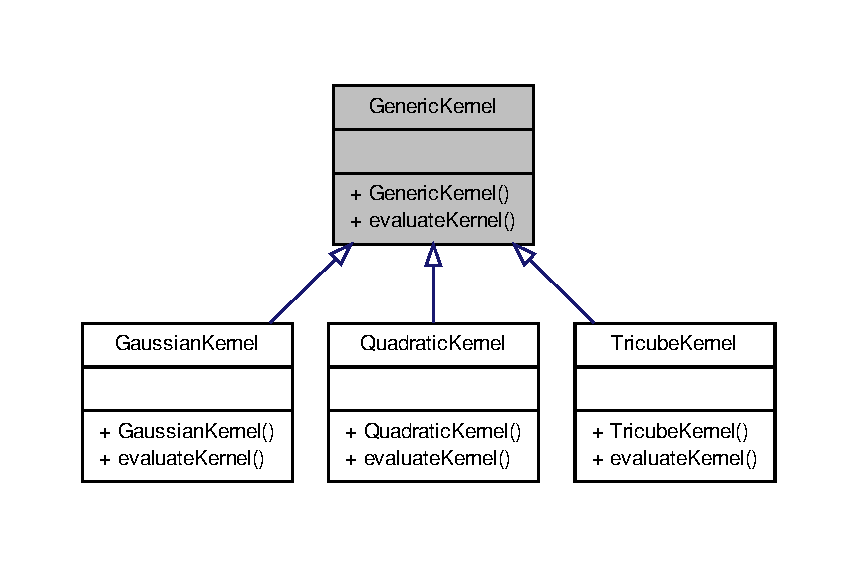
\includegraphics[width=350pt]{classGenericKernel__inherit__graph}
\end{center}
\end{figure}
\subsection*{\-Public \-Member \-Functions}
\begin{DoxyCompactItemize}
\item 
\hyperlink{classGenericKernel_abcaf5c25a540c85304912e5cf7087903}{\-Generic\-Kernel} ()
\begin{DoxyCompactList}\small\item\em constructor \end{DoxyCompactList}\item 
virtual double \hyperlink{classGenericKernel_a5b3ef309f47d56cfcb12d02bf0f0b5c7}{evaluate\-Kernel} (vec q1, vec q2, void $\ast$kernel\-Param)=0
\begin{DoxyCompactList}\small\item\em computes kernel values with given vectors q1 and q2 and passes a not further specified kernel parameter that can be used by the kernel implementation \end{DoxyCompactList}\end{DoxyCompactItemize}


\subsection{\-Detailed \-Description}
\-The \hyperlink{classGenericKernel}{\-Generic\-Kernel} class is used by the \hyperlink{classKernelRegressor}{\-Kernel\-Regressor}. \-Implementations of \hyperlink{classGenericKernel}{\-Generic\-Kernel} have to provide a certain kernel function, according to the kernel criteria. 

\subsection{\-Constructor \& \-Destructor \-Documentation}
\hypertarget{classGenericKernel_abcaf5c25a540c85304912e5cf7087903}{\index{\-Generic\-Kernel@{\-Generic\-Kernel}!\-Generic\-Kernel@{\-Generic\-Kernel}}
\index{\-Generic\-Kernel@{\-Generic\-Kernel}!GenericKernel@{\-Generic\-Kernel}}
\subsubsection[{\-Generic\-Kernel}]{\setlength{\rightskip}{0pt plus 5cm}{\bf \-Generic\-Kernel\-::\-Generic\-Kernel} (
\begin{DoxyParamCaption}
{}
\end{DoxyParamCaption}
)}}\label{classGenericKernel_abcaf5c25a540c85304912e5cf7087903}


\subsection{\-Member \-Function \-Documentation}
\hypertarget{classGenericKernel_a5b3ef309f47d56cfcb12d02bf0f0b5c7}{\index{\-Generic\-Kernel@{\-Generic\-Kernel}!evaluate\-Kernel@{evaluate\-Kernel}}
\index{evaluate\-Kernel@{evaluate\-Kernel}!GenericKernel@{\-Generic\-Kernel}}
\subsubsection[{evaluate\-Kernel}]{\setlength{\rightskip}{0pt plus 5cm}virtual double {\bf \-Generic\-Kernel\-::evaluate\-Kernel} (
\begin{DoxyParamCaption}
\item[{vec}]{q1, }
\item[{vec}]{q2, }
\item[{void $\ast$}]{kernel\-Param}
\end{DoxyParamCaption}
)\hspace{0.3cm}{\ttfamily  \mbox{[}pure virtual\mbox{]}}}}\label{classGenericKernel_a5b3ef309f47d56cfcb12d02bf0f0b5c7}

\begin{DoxyParams}{\-Parameters}
{\em q1} & vector q1 with \-K = \-K(d(q1, q2)) \\
\hline
{\em q2} & vector q2 with \-K = \-K(d(q1, q2)) \\
\hline
{\em kernel\-Param} & arbitrary kernel parameter \\
\hline
\end{DoxyParams}


\-Implemented in \hyperlink{classGaussianKernel_a11e2ca51c88c8167b86c571187995d47}{\-Gaussian\-Kernel}, \hyperlink{classQuadraticKernel_a0e7260845bf72f6fb61722cfe7c4b984}{\-Quadratic\-Kernel}, and \hyperlink{classTricubeKernel_a53a425369baf0bb3e556a08a024baf5c}{\-Tricube\-Kernel}.



\-The documentation for this class was generated from the following files\-:\begin{DoxyCompactItemize}
\item 
/home/shangl/data/data\-\_\-synched/studium/informatik/master/master\-\_\-thesis/kukadu\-\_\-framework/thesis/src/learning/\hyperlink{GenericKernel_8h}{\-Generic\-Kernel.\-h}\item 
/home/shangl/data/data\-\_\-synched/studium/informatik/master/master\-\_\-thesis/kukadu\-\_\-framework/thesis/src/learning/\hyperlink{GenericKernel_8cpp}{\-Generic\-Kernel.\-cpp}\end{DoxyCompactItemize}

\hypertarget{classGnuplotException}{\section{\-Gnuplot\-Exception \-Class \-Reference}
\label{classGnuplotException}\index{\-Gnuplot\-Exception@{\-Gnuplot\-Exception}}
}


\-A \-C++ interface to gnuplot.  




{\ttfamily \#include $<$gnuplot\-\_\-i.\-hpp$>$}

\subsection*{\-Public \-Member \-Functions}
\begin{DoxyCompactItemize}
\item 
\hyperlink{classGnuplotException_a8b324a9ef4d3f75079d41ecd61c62d44}{\-Gnuplot\-Exception} (const std\-::string \&msg)
\end{DoxyCompactItemize}


\subsection{\-Detailed \-Description}
\-The interface uses pipes and so won't run on a system that doesn't have \-P\-O\-S\-I\-X pipe support \-Tested on \-Windows (\-Min\-G\-W and \-Visual \-C++) and \-Linux (\-G\-C\-C)

\-Version history\-: 0. \-C interface by \-N. \-Devillard (27/01/03) 1. \-C++ interface\-: direct translation from the \-C interface by \-Rajarshi \-Guha (07/03/03) 2. corrections for \-Win32 compatibility by \-V. \-Chyzhdzenka (20/05/03) 3. some member functions added, corrections for \-Win32 and \-Linux compatibility by \-M. \-Burgis (10/03/08)

\-Requirements\-: gnuplot has to be installed (\href{http://www.gnuplot.info/download.html}{\tt http\-://www.\-gnuplot.\-info/download.\-html}) for \-Windows\-: set \-Path-\/\-Variable for \-Gnuplot path (e.\-g. \-C\-:/program files/gnuplot/bin) or set \-Gnuplot path with\-: \-Gnuplot\-::set\-\_\-\-G\-N\-U\-Plot\-Path(const std\-::string \&path); 

\subsection{\-Constructor \& \-Destructor \-Documentation}
\hypertarget{classGnuplotException_a8b324a9ef4d3f75079d41ecd61c62d44}{\index{\-Gnuplot\-Exception@{\-Gnuplot\-Exception}!\-Gnuplot\-Exception@{\-Gnuplot\-Exception}}
\index{\-Gnuplot\-Exception@{\-Gnuplot\-Exception}!GnuplotException@{\-Gnuplot\-Exception}}
\subsubsection[{\-Gnuplot\-Exception}]{\setlength{\rightskip}{0pt plus 5cm}{\bf \-Gnuplot\-Exception\-::\-Gnuplot\-Exception} (
\begin{DoxyParamCaption}
\item[{const std\-::string \&}]{msg}
\end{DoxyParamCaption}
)\hspace{0.3cm}{\ttfamily  \mbox{[}inline\mbox{]}}}}\label{classGnuplotException_a8b324a9ef4d3f75079d41ecd61c62d44}


\-The documentation for this class was generated from the following file\-:\begin{DoxyCompactItemize}
\item 
/home/shangl/data/data\-\_\-synched/studium/informatik/master/master\-\_\-thesis/kukadu\-\_\-framework/thesis/src/utils/gnuplot-\/cpp/\hyperlink{gnuplot__i_8hpp}{gnuplot\-\_\-i.\-hpp}\end{DoxyCompactItemize}

\hypertarget{classKernelRegressor}{\section{\-Kernel\-Regressor \-Class \-Reference}
\label{classKernelRegressor}\index{\-Kernel\-Regressor@{\-Kernel\-Regressor}}
}


\-Provides arbitrary interface for kernel methods.  




{\ttfamily \#include $<$\-Kernel\-Regressor.\-h$>$}



\-Inheritance diagram for \-Kernel\-Regressor\-:\nopagebreak
\begin{figure}[H]
\begin{center}
\leavevmode
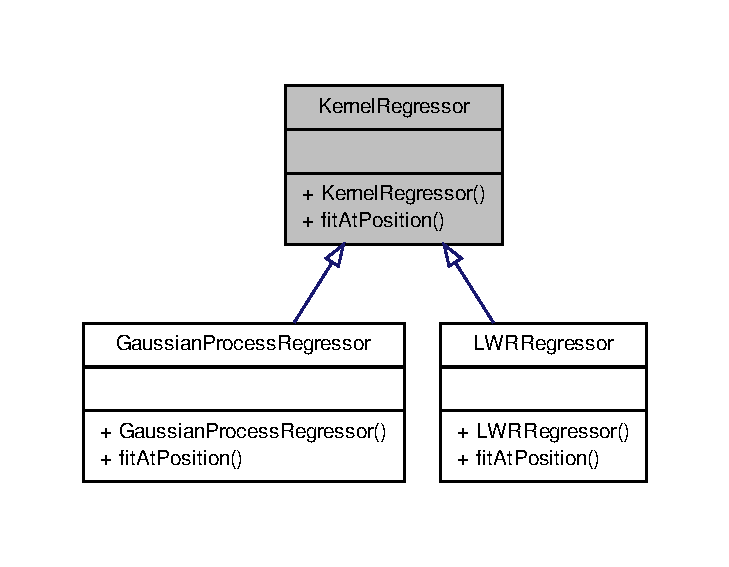
\includegraphics[width=350pt]{classKernelRegressor__inherit__graph}
\end{center}
\end{figure}
\subsection*{\-Public \-Member \-Functions}
\begin{DoxyCompactItemize}
\item 
\hyperlink{classKernelRegressor_a4dc472698406ed91148f7245d4c41687}{\-Kernel\-Regressor} ()
\begin{DoxyCompactList}\small\item\em constructor \end{DoxyCompactList}\item 
virtual vec \hyperlink{classKernelRegressor_a65529e1d764f9abf0498c93a35ac3f16}{fit\-At\-Position} (vec pos)=0
\begin{DoxyCompactList}\small\item\em performs the kernel method for predicting the functin value at a given position \end{DoxyCompactList}\end{DoxyCompactItemize}


\subsection{\-Detailed \-Description}
\-This class provides the interface for kernel machine learning methods such as \-Gaussian process regression or locally weighted regression 

\subsection{\-Constructor \& \-Destructor \-Documentation}
\hypertarget{classKernelRegressor_a4dc472698406ed91148f7245d4c41687}{\index{\-Kernel\-Regressor@{\-Kernel\-Regressor}!\-Kernel\-Regressor@{\-Kernel\-Regressor}}
\index{\-Kernel\-Regressor@{\-Kernel\-Regressor}!KernelRegressor@{\-Kernel\-Regressor}}
\subsubsection[{\-Kernel\-Regressor}]{\setlength{\rightskip}{0pt plus 5cm}{\bf \-Kernel\-Regressor\-::\-Kernel\-Regressor} (
\begin{DoxyParamCaption}
{}
\end{DoxyParamCaption}
)}}\label{classKernelRegressor_a4dc472698406ed91148f7245d4c41687}


\subsection{\-Member \-Function \-Documentation}
\hypertarget{classKernelRegressor_a65529e1d764f9abf0498c93a35ac3f16}{\index{\-Kernel\-Regressor@{\-Kernel\-Regressor}!fit\-At\-Position@{fit\-At\-Position}}
\index{fit\-At\-Position@{fit\-At\-Position}!KernelRegressor@{\-Kernel\-Regressor}}
\subsubsection[{fit\-At\-Position}]{\setlength{\rightskip}{0pt plus 5cm}virtual vec {\bf \-Kernel\-Regressor\-::fit\-At\-Position} (
\begin{DoxyParamCaption}
\item[{vec}]{pos}
\end{DoxyParamCaption}
)\hspace{0.3cm}{\ttfamily  \mbox{[}pure virtual\mbox{]}}}}\label{classKernelRegressor_a65529e1d764f9abf0498c93a35ac3f16}

\begin{DoxyParams}{\-Parameters}
{\em pos} & vector defining the required position \\
\hline
\end{DoxyParams}


\-Implemented in \hyperlink{classLWRRegressor_aea55827ce2c63078414469fe21c16f23}{\-L\-W\-R\-Regressor}, and \hyperlink{classGaussianProcessRegressor_a9c4ad88ae6cbbc457cbfa17c64e59d1b}{\-Gaussian\-Process\-Regressor}.



\-The documentation for this class was generated from the following files\-:\begin{DoxyCompactItemize}
\item 
/home/shangl/data/data\-\_\-synched/studium/informatik/master/master\-\_\-thesis/kukadu\-\_\-framework/thesis/src/learning/\hyperlink{KernelRegressor_8h}{\-Kernel\-Regressor.\-h}\item 
/home/shangl/data/data\-\_\-synched/studium/informatik/master/master\-\_\-thesis/kukadu\-\_\-framework/thesis/src/learning/\hyperlink{KernelRegressor_8cpp}{\-Kernel\-Regressor.\-cpp}\end{DoxyCompactItemize}

\hypertarget{classKukaControlQueue}{\section{\-Kuka\-Control\-Queue \-Class \-Reference}
\label{classKukaControlQueue}\index{\-Kuka\-Control\-Queue@{\-Kuka\-Control\-Queue}}
}


\-The \hyperlink{classKukaControlQueue}{\-Kuka\-Control\-Queue} provides control capabilities for the \-Kuka \-L\-W\-R 4+ robotic arm.  




{\ttfamily \#include $<$\-Kuka\-Control\-Queue.\-h$>$}



\-Inheritance diagram for \-Kuka\-Control\-Queue\-:\nopagebreak
\begin{figure}[H]
\begin{center}
\leavevmode
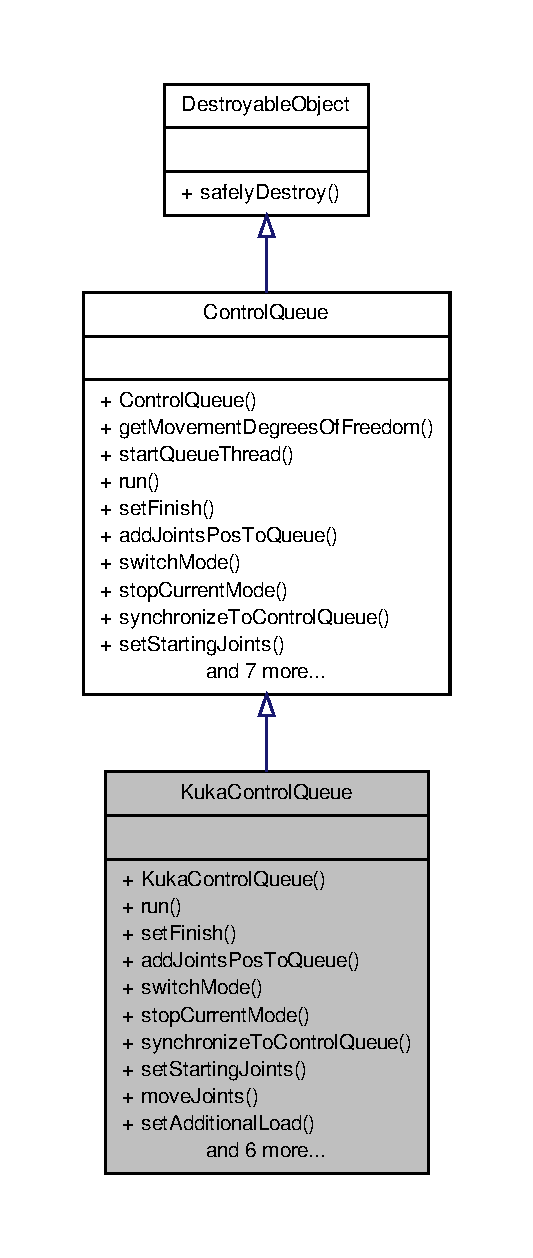
\includegraphics[height=550pt]{classKukaControlQueue__inherit__graph}
\end{center}
\end{figure}


\-Collaboration diagram for \-Kuka\-Control\-Queue\-:\nopagebreak
\begin{figure}[H]
\begin{center}
\leavevmode
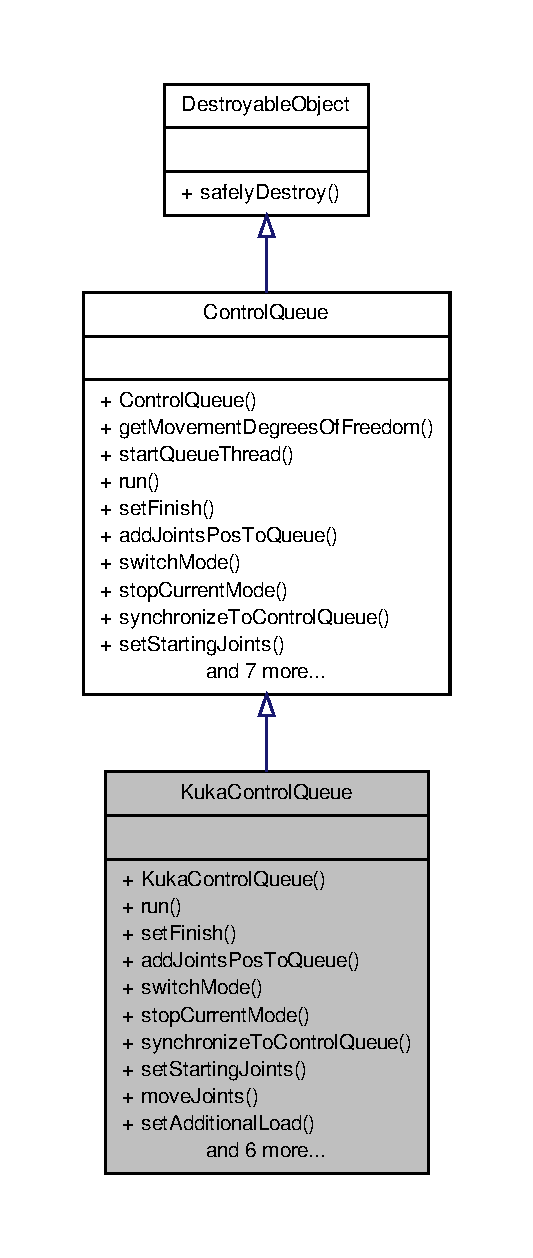
\includegraphics[height=550pt]{classKukaControlQueue__coll__graph}
\end{center}
\end{figure}
\subsection*{\-Public \-Member \-Functions}
\begin{DoxyCompactItemize}
\item 
\hyperlink{classKukaControlQueue_ad83b88087dd9cec8c52e3211af54013c}{\-Kuka\-Control\-Queue} (int port, int sleep\-Time, int init\-Mode)
\begin{DoxyCompactList}\small\item\em \-Constructor for \hyperlink{classKukaControlQueue}{\-Kuka\-Control\-Queue}. \end{DoxyCompactList}\item 
void \hyperlink{classKukaControlQueue_ac77a50c65dd633fa18913c45cc6fe26a}{run} ()
\begin{DoxyCompactList}\small\item\em \-This method is started in a new thread by start\-Queue. \end{DoxyCompactList}\item 
void \hyperlink{classKukaControlQueue_aac151fe8a3fb3e2744ea29ef37036754}{set\-Finish} ()
\begin{DoxyCompactList}\small\item\em \-Sets a flag to stop the control thread after current iteration is executed. \end{DoxyCompactList}\item 
void \hyperlink{classKukaControlQueue_a62ccf60f8a53d8d04a14a4d396b3d13a}{add\-Joints\-Pos\-To\-Queue} (float $\ast$\hyperlink{fri__example_8m_a094bd681592faefb6f9be3d22d34cbcd}{joints})
\begin{DoxyCompactList}\small\item\em \-Adds next joint position to queue. \end{DoxyCompactList}\item 
void \hyperlink{classKukaControlQueue_a8bbf6b7c4a0cea73c4e3891d18d51fdf}{switch\-Mode} (int mode)
\begin{DoxyCompactList}\small\item\em \-Switches robot modes. \-A state might be a real time command mode or an monitoring mode. \end{DoxyCompactList}\item 
void \hyperlink{classKukaControlQueue_a33c03e1a8b1e5fef533a6cdaca9fe15d}{stop\-Current\-Mode} ()
\begin{DoxyCompactList}\small\item\em \-Stops current mode and switches back to default mode (e.\-g. monitoring mode) \end{DoxyCompactList}\item 
void \hyperlink{classKukaControlQueue_a3e59c3d253d2306b5fdde56da529c9cd}{synchronize\-To\-Control\-Queue} (int max\-Num\-Joints\-In\-Queue)
\begin{DoxyCompactList}\small\item\em \-Blocks, if more than the defined maximum element count is in the queue. \end{DoxyCompactList}\item 
void \hyperlink{classKukaControlQueue_ae9b6465ad4c714b305af4eb0b8e69584}{set\-Starting\-Joints} (float $\ast$\hyperlink{fri__example_8m_a094bd681592faefb6f9be3d22d34cbcd}{joints})
\begin{DoxyCompactList}\small\item\em \-Sets joints in which the should be in before robot enters command mode. \end{DoxyCompactList}\item 
void \hyperlink{classKukaControlQueue_a2b9e7cfb4918201e1da5e2a365395e46}{move\-Joints} (float $\ast$\hyperlink{fri__example_8m_a094bd681592faefb6f9be3d22d34cbcd}{joints})
\begin{DoxyCompactList}\small\item\em \-Implements simple point to point movement in joint space. \end{DoxyCompactList}\item 
void \hyperlink{classKukaControlQueue_a0c6a2edd22e222c672668fac5cacb55a}{set\-Additional\-Load} (float load\-Mass, float load\-Pos)
\begin{DoxyCompactList}\small\item\em \-Changes the load data of the robot (e.\-g. needs to be used whenever robot picks up an object) \end{DoxyCompactList}\item 
void \hyperlink{classKukaControlQueue_a82c93a4979d678344337461dd9084725}{set\-Stiffness} (float cpstiffnessxyz, float cpstiffnessabc, float cpdamping, float cpmaxdelta, float maxforce, float axismaxdeltatrq)
\begin{DoxyCompactList}\small\item\em \-Sets certain stiffness parameters in cartesian space (if the robot supports this) according to a mass spring damper system model. \end{DoxyCompactList}\item 
float $\ast$ \hyperlink{classKukaControlQueue_a62475e2d6fd485bfbce095d67bab96c6}{get\-Cartesian\-Pos} ()
\begin{DoxyCompactList}\small\item\em \-Returns current robot position in cartesian space. \end{DoxyCompactList}\item 
float $\ast$ \hyperlink{classKukaControlQueue_a53c5b0fe118ce0847586ccccc1481edb}{get\-Starting\-Joints} ()
\begin{DoxyCompactList}\small\item\em \-Returns the robot joints the robot has been directly before starting command mode. \end{DoxyCompactList}\item 
float $\ast$ \hyperlink{classKukaControlQueue_a4d426306e965f9e81cdad5b10229866f}{retrieve\-Joints\-From\-Robot} ()
\begin{DoxyCompactList}\small\item\em \-Returns joints if the robot is in monitor mode. \end{DoxyCompactList}\item 
mes\-\_\-result \hyperlink{classKukaControlQueue_a363040926a2e014b347cc7016b639f25}{get\-Current\-Joints} ()
\begin{DoxyCompactList}\small\item\em \-Returns joints if the robot is in command mode. \end{DoxyCompactList}\item 
bool \hyperlink{classKukaControlQueue_ae7844ed3c8210152dd0b4a97e9c9f7a6}{is\-Initialized} ()
\begin{DoxyCompactList}\small\item\em \-Returns true if the command mode initialization is done. \end{DoxyCompactList}\item 
void \hyperlink{classKukaControlQueue_ad086a60270e8c6b56c3e09aa1c595b4e}{safely\-Destroy} ()
\begin{DoxyCompactList}\small\item\em \-Method is called whenever destroy event occurs and ensures safe and clean termination of the programm (e.\-g. stops robot) \end{DoxyCompactList}\end{DoxyCompactItemize}


\subsection{\-Detailed \-Description}
\-This class implements the abstract \hyperlink{classControlQueue}{\-Control\-Queue} class for the usage with the \-Kuka \-L\-W\-R 4+ robotic arm. \-It provides basic functionalities such as command mode control in joint space as well as point to point movement in cartesian and joint space. \-To use it, the additionally provided \-K\-R\-L script has to be selected on the robot controller side. \-For further information how to use it, please see the sample programs and the kuka documentation 

\subsection{\-Constructor \& \-Destructor \-Documentation}
\hypertarget{classKukaControlQueue_ad83b88087dd9cec8c52e3211af54013c}{\index{\-Kuka\-Control\-Queue@{\-Kuka\-Control\-Queue}!\-Kuka\-Control\-Queue@{\-Kuka\-Control\-Queue}}
\index{\-Kuka\-Control\-Queue@{\-Kuka\-Control\-Queue}!KukaControlQueue@{\-Kuka\-Control\-Queue}}
\subsubsection[{\-Kuka\-Control\-Queue}]{\setlength{\rightskip}{0pt plus 5cm}{\bf \-Kuka\-Control\-Queue\-::\-Kuka\-Control\-Queue} (
\begin{DoxyParamCaption}
\item[{int}]{port, }
\item[{int}]{sleep\-Time, }
\item[{int}]{init\-Mode}
\end{DoxyParamCaption}
)}}\label{classKukaControlQueue_ad83b88087dd9cec8c52e3211af54013c}

\begin{DoxyParams}{\-Parameters}
{\em port} & port to listen for incoming fri connection \\
\hline
{\em sleep\-Time} & cycle sleep time (time between to packets sent in command mode) \\
\hline
{\em init\-Mode} & control mode (e.\-g. command mode, monitor mode) with which the queue should be started \\
\hline
\end{DoxyParams}


\subsection{\-Member \-Function \-Documentation}
\hypertarget{classKukaControlQueue_a62ccf60f8a53d8d04a14a4d396b3d13a}{\index{\-Kuka\-Control\-Queue@{\-Kuka\-Control\-Queue}!add\-Joints\-Pos\-To\-Queue@{add\-Joints\-Pos\-To\-Queue}}
\index{add\-Joints\-Pos\-To\-Queue@{add\-Joints\-Pos\-To\-Queue}!KukaControlQueue@{\-Kuka\-Control\-Queue}}
\subsubsection[{add\-Joints\-Pos\-To\-Queue}]{\setlength{\rightskip}{0pt plus 5cm}void {\bf \-Kuka\-Control\-Queue\-::add\-Joints\-Pos\-To\-Queue} (
\begin{DoxyParamCaption}
\item[{float $\ast$}]{joints}
\end{DoxyParamCaption}
)\hspace{0.3cm}{\ttfamily  \mbox{[}virtual\mbox{]}}}}\label{classKukaControlQueue_a62ccf60f8a53d8d04a14a4d396b3d13a}

\begin{DoxyParams}{\-Parameters}
{\em joints} & joints to add \\
\hline
\end{DoxyParams}


\-Implements \hyperlink{classControlQueue_a8750612f82e110cb5378672d6f64ca6f}{\-Control\-Queue}.

\hypertarget{classKukaControlQueue_a62475e2d6fd485bfbce095d67bab96c6}{\index{\-Kuka\-Control\-Queue@{\-Kuka\-Control\-Queue}!get\-Cartesian\-Pos@{get\-Cartesian\-Pos}}
\index{get\-Cartesian\-Pos@{get\-Cartesian\-Pos}!KukaControlQueue@{\-Kuka\-Control\-Queue}}
\subsubsection[{get\-Cartesian\-Pos}]{\setlength{\rightskip}{0pt plus 5cm}float $\ast$ {\bf \-Kuka\-Control\-Queue\-::get\-Cartesian\-Pos} (
\begin{DoxyParamCaption}
{}
\end{DoxyParamCaption}
)\hspace{0.3cm}{\ttfamily  \mbox{[}virtual\mbox{]}}}}\label{classKukaControlQueue_a62475e2d6fd485bfbce095d67bab96c6}


\-Implements \hyperlink{classControlQueue_a9bdc3efe662d9d275d48ec523627ef7c}{\-Control\-Queue}.

\hypertarget{classKukaControlQueue_a363040926a2e014b347cc7016b639f25}{\index{\-Kuka\-Control\-Queue@{\-Kuka\-Control\-Queue}!get\-Current\-Joints@{get\-Current\-Joints}}
\index{get\-Current\-Joints@{get\-Current\-Joints}!KukaControlQueue@{\-Kuka\-Control\-Queue}}
\subsubsection[{get\-Current\-Joints}]{\setlength{\rightskip}{0pt plus 5cm}mes\-\_\-result {\bf \-Kuka\-Control\-Queue\-::get\-Current\-Joints} (
\begin{DoxyParamCaption}
{}
\end{DoxyParamCaption}
)\hspace{0.3cm}{\ttfamily  \mbox{[}virtual\mbox{]}}}}\label{classKukaControlQueue_a363040926a2e014b347cc7016b639f25}


\-Implements \hyperlink{classControlQueue_aa610fa7b8b53ed7c406eba1fa4eb106c}{\-Control\-Queue}.

\hypertarget{classKukaControlQueue_a53c5b0fe118ce0847586ccccc1481edb}{\index{\-Kuka\-Control\-Queue@{\-Kuka\-Control\-Queue}!get\-Starting\-Joints@{get\-Starting\-Joints}}
\index{get\-Starting\-Joints@{get\-Starting\-Joints}!KukaControlQueue@{\-Kuka\-Control\-Queue}}
\subsubsection[{get\-Starting\-Joints}]{\setlength{\rightskip}{0pt plus 5cm}float $\ast$ {\bf \-Kuka\-Control\-Queue\-::get\-Starting\-Joints} (
\begin{DoxyParamCaption}
{}
\end{DoxyParamCaption}
)\hspace{0.3cm}{\ttfamily  \mbox{[}virtual\mbox{]}}}}\label{classKukaControlQueue_a53c5b0fe118ce0847586ccccc1481edb}


\-Implements \hyperlink{classControlQueue_a4b8c95e38791477bf925ac8f61c38821}{\-Control\-Queue}.

\hypertarget{classKukaControlQueue_ae7844ed3c8210152dd0b4a97e9c9f7a6}{\index{\-Kuka\-Control\-Queue@{\-Kuka\-Control\-Queue}!is\-Initialized@{is\-Initialized}}
\index{is\-Initialized@{is\-Initialized}!KukaControlQueue@{\-Kuka\-Control\-Queue}}
\subsubsection[{is\-Initialized}]{\setlength{\rightskip}{0pt plus 5cm}bool {\bf \-Kuka\-Control\-Queue\-::is\-Initialized} (
\begin{DoxyParamCaption}
{}
\end{DoxyParamCaption}
)\hspace{0.3cm}{\ttfamily  \mbox{[}virtual\mbox{]}}}}\label{classKukaControlQueue_ae7844ed3c8210152dd0b4a97e9c9f7a6}


\-Implements \hyperlink{classControlQueue_a153ff04f335b33580d15d2e16f17265b}{\-Control\-Queue}.

\hypertarget{classKukaControlQueue_a2b9e7cfb4918201e1da5e2a365395e46}{\index{\-Kuka\-Control\-Queue@{\-Kuka\-Control\-Queue}!move\-Joints@{move\-Joints}}
\index{move\-Joints@{move\-Joints}!KukaControlQueue@{\-Kuka\-Control\-Queue}}
\subsubsection[{move\-Joints}]{\setlength{\rightskip}{0pt plus 5cm}void {\bf \-Kuka\-Control\-Queue\-::move\-Joints} (
\begin{DoxyParamCaption}
\item[{float $\ast$}]{joints}
\end{DoxyParamCaption}
)\hspace{0.3cm}{\ttfamily  \mbox{[}virtual\mbox{]}}}}\label{classKukaControlQueue_a2b9e7cfb4918201e1da5e2a365395e46}

\begin{DoxyParams}{\-Parameters}
{\em joints} & array of joint positions \\
\hline
\end{DoxyParams}


\-Implements \hyperlink{classControlQueue_ac42d07279bbbf5f72928955ea71a407f}{\-Control\-Queue}.

\hypertarget{classKukaControlQueue_a4d426306e965f9e81cdad5b10229866f}{\index{\-Kuka\-Control\-Queue@{\-Kuka\-Control\-Queue}!retrieve\-Joints\-From\-Robot@{retrieve\-Joints\-From\-Robot}}
\index{retrieve\-Joints\-From\-Robot@{retrieve\-Joints\-From\-Robot}!KukaControlQueue@{\-Kuka\-Control\-Queue}}
\subsubsection[{retrieve\-Joints\-From\-Robot}]{\setlength{\rightskip}{0pt plus 5cm}float $\ast$ {\bf \-Kuka\-Control\-Queue\-::retrieve\-Joints\-From\-Robot} (
\begin{DoxyParamCaption}
{}
\end{DoxyParamCaption}
)\hspace{0.3cm}{\ttfamily  \mbox{[}virtual\mbox{]}}}}\label{classKukaControlQueue_a4d426306e965f9e81cdad5b10229866f}


\-Implements \hyperlink{classControlQueue_a7b803a4b12bfa70c79fdad108e63b0f4}{\-Control\-Queue}.

\hypertarget{classKukaControlQueue_ac77a50c65dd633fa18913c45cc6fe26a}{\index{\-Kuka\-Control\-Queue@{\-Kuka\-Control\-Queue}!run@{run}}
\index{run@{run}!KukaControlQueue@{\-Kuka\-Control\-Queue}}
\subsubsection[{run}]{\setlength{\rightskip}{0pt plus 5cm}void {\bf \-Kuka\-Control\-Queue\-::run} (
\begin{DoxyParamCaption}
{}
\end{DoxyParamCaption}
)\hspace{0.3cm}{\ttfamily  \mbox{[}virtual\mbox{]}}}}\label{classKukaControlQueue_ac77a50c65dd633fa18913c45cc6fe26a}


\-Implements \hyperlink{classControlQueue_a532fc65ff27e37e35078ae2ccc54e408}{\-Control\-Queue}.

\hypertarget{classKukaControlQueue_ad086a60270e8c6b56c3e09aa1c595b4e}{\index{\-Kuka\-Control\-Queue@{\-Kuka\-Control\-Queue}!safely\-Destroy@{safely\-Destroy}}
\index{safely\-Destroy@{safely\-Destroy}!KukaControlQueue@{\-Kuka\-Control\-Queue}}
\subsubsection[{safely\-Destroy}]{\setlength{\rightskip}{0pt plus 5cm}void {\bf \-Kuka\-Control\-Queue\-::safely\-Destroy} (
\begin{DoxyParamCaption}
{}
\end{DoxyParamCaption}
)\hspace{0.3cm}{\ttfamily  \mbox{[}virtual\mbox{]}}}}\label{classKukaControlQueue_ad086a60270e8c6b56c3e09aa1c595b4e}


\-Implements \hyperlink{classDestroyableObject_a728d19d81eca540efd68650867f197be}{\-Destroyable\-Object}.

\hypertarget{classKukaControlQueue_a0c6a2edd22e222c672668fac5cacb55a}{\index{\-Kuka\-Control\-Queue@{\-Kuka\-Control\-Queue}!set\-Additional\-Load@{set\-Additional\-Load}}
\index{set\-Additional\-Load@{set\-Additional\-Load}!KukaControlQueue@{\-Kuka\-Control\-Queue}}
\subsubsection[{set\-Additional\-Load}]{\setlength{\rightskip}{0pt plus 5cm}void {\bf \-Kuka\-Control\-Queue\-::set\-Additional\-Load} (
\begin{DoxyParamCaption}
\item[{float}]{load\-Mass, }
\item[{float}]{load\-Pos}
\end{DoxyParamCaption}
)\hspace{0.3cm}{\ttfamily  \mbox{[}virtual\mbox{]}}}}\label{classKukaControlQueue_a0c6a2edd22e222c672668fac5cacb55a}

\begin{DoxyParams}{\-Parameters}
{\em load\-Mass} & mass of the picked up object \\
\hline
{\em load\-Pos} & position of the objects center of gravity relative to the manipulator \\
\hline
\end{DoxyParams}


\-Implements \hyperlink{classControlQueue_ae34e58840111692913a45ccde7b6fc20}{\-Control\-Queue}.

\hypertarget{classKukaControlQueue_aac151fe8a3fb3e2744ea29ef37036754}{\index{\-Kuka\-Control\-Queue@{\-Kuka\-Control\-Queue}!set\-Finish@{set\-Finish}}
\index{set\-Finish@{set\-Finish}!KukaControlQueue@{\-Kuka\-Control\-Queue}}
\subsubsection[{set\-Finish}]{\setlength{\rightskip}{0pt plus 5cm}void {\bf \-Kuka\-Control\-Queue\-::set\-Finish} (
\begin{DoxyParamCaption}
{}
\end{DoxyParamCaption}
)\hspace{0.3cm}{\ttfamily  \mbox{[}virtual\mbox{]}}}}\label{classKukaControlQueue_aac151fe8a3fb3e2744ea29ef37036754}


\-Implements \hyperlink{classControlQueue_a07626e6ef2bdf7e5fe59a2548ab0a213}{\-Control\-Queue}.

\hypertarget{classKukaControlQueue_ae9b6465ad4c714b305af4eb0b8e69584}{\index{\-Kuka\-Control\-Queue@{\-Kuka\-Control\-Queue}!set\-Starting\-Joints@{set\-Starting\-Joints}}
\index{set\-Starting\-Joints@{set\-Starting\-Joints}!KukaControlQueue@{\-Kuka\-Control\-Queue}}
\subsubsection[{set\-Starting\-Joints}]{\setlength{\rightskip}{0pt plus 5cm}void {\bf \-Kuka\-Control\-Queue\-::set\-Starting\-Joints} (
\begin{DoxyParamCaption}
\item[{float $\ast$}]{joints}
\end{DoxyParamCaption}
)\hspace{0.3cm}{\ttfamily  \mbox{[}virtual\mbox{]}}}}\label{classKukaControlQueue_ae9b6465ad4c714b305af4eb0b8e69584}

\begin{DoxyParams}{\-Parameters}
{\em joints} & array of joint positions \\
\hline
\end{DoxyParams}


\-Implements \hyperlink{classControlQueue_ad63c9ae478a918b3e60cedbe89f78054}{\-Control\-Queue}.

\hypertarget{classKukaControlQueue_a82c93a4979d678344337461dd9084725}{\index{\-Kuka\-Control\-Queue@{\-Kuka\-Control\-Queue}!set\-Stiffness@{set\-Stiffness}}
\index{set\-Stiffness@{set\-Stiffness}!KukaControlQueue@{\-Kuka\-Control\-Queue}}
\subsubsection[{set\-Stiffness}]{\setlength{\rightskip}{0pt plus 5cm}void {\bf \-Kuka\-Control\-Queue\-::set\-Stiffness} (
\begin{DoxyParamCaption}
\item[{float}]{cpstiffnessxyz, }
\item[{float}]{cpstiffnessabc, }
\item[{float}]{cpdamping, }
\item[{float}]{cpmaxdelta, }
\item[{float}]{maxforce, }
\item[{float}]{axismaxdeltatrq}
\end{DoxyParamCaption}
)\hspace{0.3cm}{\ttfamily  \mbox{[}virtual\mbox{]}}}}\label{classKukaControlQueue_a82c93a4979d678344337461dd9084725}

\begin{DoxyParams}{\-Parameters}
{\em cpstiffnessxyz} & stiffness of the robot in the cartesian space \\
\hline
{\em cpstiffnessabc} & stiffness of the rotational axis of the tool mounting point in cartesian space \\
\hline
{\em cpdamping} & damping of the robots axis in cartesian space \\
\hline
{\em cpmaxdelta} & maximum allows deviation in cartesian space \\
\hline
{\em maxforce} & maximum allowed applied force \\
\hline
{\em axismaxdeltatrq} & maximum allowed applied torque \\
\hline
\end{DoxyParams}


\-Implements \hyperlink{classControlQueue_ad6d5bccd9d08d40d5464f10a958e5328}{\-Control\-Queue}.

\hypertarget{classKukaControlQueue_a33c03e1a8b1e5fef533a6cdaca9fe15d}{\index{\-Kuka\-Control\-Queue@{\-Kuka\-Control\-Queue}!stop\-Current\-Mode@{stop\-Current\-Mode}}
\index{stop\-Current\-Mode@{stop\-Current\-Mode}!KukaControlQueue@{\-Kuka\-Control\-Queue}}
\subsubsection[{stop\-Current\-Mode}]{\setlength{\rightskip}{0pt plus 5cm}void {\bf \-Kuka\-Control\-Queue\-::stop\-Current\-Mode} (
\begin{DoxyParamCaption}
{}
\end{DoxyParamCaption}
)\hspace{0.3cm}{\ttfamily  \mbox{[}virtual\mbox{]}}}}\label{classKukaControlQueue_a33c03e1a8b1e5fef533a6cdaca9fe15d}


\-Implements \hyperlink{classControlQueue_a74ed9cbabd7a9f6a62460dbd5dc9e48d}{\-Control\-Queue}.

\hypertarget{classKukaControlQueue_a8bbf6b7c4a0cea73c4e3891d18d51fdf}{\index{\-Kuka\-Control\-Queue@{\-Kuka\-Control\-Queue}!switch\-Mode@{switch\-Mode}}
\index{switch\-Mode@{switch\-Mode}!KukaControlQueue@{\-Kuka\-Control\-Queue}}
\subsubsection[{switch\-Mode}]{\setlength{\rightskip}{0pt plus 5cm}void {\bf \-Kuka\-Control\-Queue\-::switch\-Mode} (
\begin{DoxyParamCaption}
\item[{int}]{mode}
\end{DoxyParamCaption}
)\hspace{0.3cm}{\ttfamily  \mbox{[}virtual\mbox{]}}}}\label{classKukaControlQueue_a8bbf6b7c4a0cea73c4e3891d18d51fdf}

\begin{DoxyParams}{\-Parameters}
{\em mode} & mode id \\
\hline
\end{DoxyParams}


\-Implements \hyperlink{classControlQueue_a0f0367b72b6b1bd75b39aeb19db93dc5}{\-Control\-Queue}.

\hypertarget{classKukaControlQueue_a3e59c3d253d2306b5fdde56da529c9cd}{\index{\-Kuka\-Control\-Queue@{\-Kuka\-Control\-Queue}!synchronize\-To\-Control\-Queue@{synchronize\-To\-Control\-Queue}}
\index{synchronize\-To\-Control\-Queue@{synchronize\-To\-Control\-Queue}!KukaControlQueue@{\-Kuka\-Control\-Queue}}
\subsubsection[{synchronize\-To\-Control\-Queue}]{\setlength{\rightskip}{0pt plus 5cm}void {\bf \-Kuka\-Control\-Queue\-::synchronize\-To\-Control\-Queue} (
\begin{DoxyParamCaption}
\item[{int}]{max\-Num\-Joints\-In\-Queue}
\end{DoxyParamCaption}
)\hspace{0.3cm}{\ttfamily  \mbox{[}virtual\mbox{]}}}}\label{classKukaControlQueue_a3e59c3d253d2306b5fdde56da529c9cd}

\begin{DoxyParams}{\-Parameters}
{\em max\-Num\-Joints\-In\-Queue} & maximum number of joints in queue \\
\hline
\end{DoxyParams}


\-Implements \hyperlink{classControlQueue_a37493f41806df96293a95f52f23da280}{\-Control\-Queue}.



\-The documentation for this class was generated from the following files\-:\begin{DoxyCompactItemize}
\item 
/home/shangl/data/data\-\_\-synched/studium/informatik/master/master\-\_\-thesis/kukadu\-\_\-framework/thesis/src/robot/\hyperlink{KukaControlQueue_8h}{\-Kuka\-Control\-Queue.\-h}\item 
/home/shangl/data/data\-\_\-synched/studium/informatik/master/master\-\_\-thesis/kukadu\-\_\-framework/thesis/src/robot/\hyperlink{KukaControlQueue_8cpp}{\-Kuka\-Control\-Queue.\-cpp}\end{DoxyCompactItemize}

\hypertarget{classLWRRegressor}{\section{\-L\-W\-R\-Regressor \-Class \-Reference}
\label{classLWRRegressor}\index{\-L\-W\-R\-Regressor@{\-L\-W\-R\-Regressor}}
}


\-Implements the locally weighted regression method.  




{\ttfamily \#include $<$\-L\-W\-R\-Regressor.\-h$>$}



\-Inheritance diagram for \-L\-W\-R\-Regressor\-:\nopagebreak
\begin{figure}[H]
\begin{center}
\leavevmode
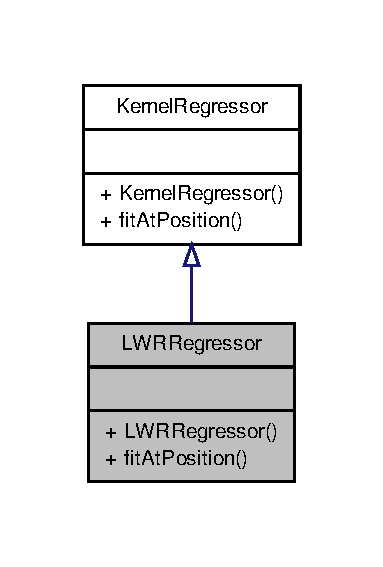
\includegraphics[width=184pt]{classLWRRegressor__inherit__graph}
\end{center}
\end{figure}


\-Collaboration diagram for \-L\-W\-R\-Regressor\-:\nopagebreak
\begin{figure}[H]
\begin{center}
\leavevmode
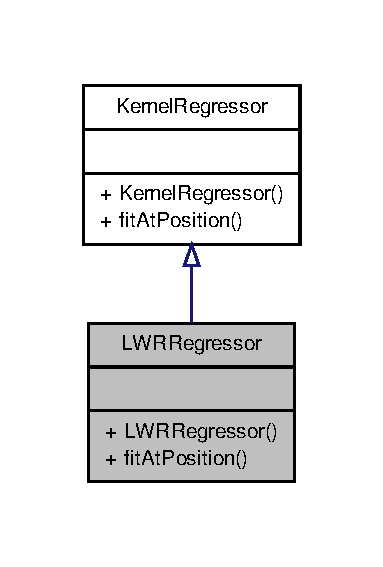
\includegraphics[width=184pt]{classLWRRegressor__coll__graph}
\end{center}
\end{figure}
\subsection*{\-Public \-Member \-Functions}
\begin{DoxyCompactItemize}
\item 
\hyperlink{classLWRRegressor_a536ce119230557df4154a2d92fdd0607}{\-L\-W\-R\-Regressor} (vector$<$ vec $>$ sample\-Xs, vector$<$ vec $>$ sample\-Ts, \hyperlink{classGenericKernel}{\-Generic\-Kernel} $\ast$kernel, vector$<$ mat $>$ design\-Matrices)
\begin{DoxyCompactList}\small\item\em constructor, setting all the sample data, the selected kernel and a vector of design matrices (one design matrix for each sample) \end{DoxyCompactList}\item 
vec \hyperlink{classLWRRegressor_aea55827ce2c63078414469fe21c16f23}{fit\-At\-Position} (vec pos)
\begin{DoxyCompactList}\small\item\em performs the kernel method for predicting the functin value at a given position \end{DoxyCompactList}\end{DoxyCompactItemize}


\subsection{\-Detailed \-Description}
\-This class inherits from the \hyperlink{classKernelRegressor}{\-Kernel\-Regressor} and implements locally weighted regression. \-It reuses the design matrices computed by the \hyperlink{classGeneralFitter}{\-General\-Fitter} class. 

\subsection{\-Constructor \& \-Destructor \-Documentation}
\hypertarget{classLWRRegressor_a536ce119230557df4154a2d92fdd0607}{\index{\-L\-W\-R\-Regressor@{\-L\-W\-R\-Regressor}!\-L\-W\-R\-Regressor@{\-L\-W\-R\-Regressor}}
\index{\-L\-W\-R\-Regressor@{\-L\-W\-R\-Regressor}!LWRRegressor@{\-L\-W\-R\-Regressor}}
\subsubsection[{\-L\-W\-R\-Regressor}]{\setlength{\rightskip}{0pt plus 5cm}{\bf \-L\-W\-R\-Regressor\-::\-L\-W\-R\-Regressor} (
\begin{DoxyParamCaption}
\item[{vector$<$ vec $>$}]{sample\-Xs, }
\item[{vector$<$ vec $>$}]{sample\-Ts, }
\item[{{\bf \-Generic\-Kernel} $\ast$}]{kernel, }
\item[{vector$<$ mat $>$}]{design\-Matrices}
\end{DoxyParamCaption}
)}}\label{classLWRRegressor_a536ce119230557df4154a2d92fdd0607}

\begin{DoxyParams}{\-Parameters}
{\em sample\-Xs} & vector of samples (x-\/axis) \\
\hline
{\em sample\-Ts} & vector of samples (y-\/axis) \\
\hline
{\em kernel} & the selected kernel implementation \\
\hline
{\em design\-Matrices} & vector of design matrices \\
\hline
\end{DoxyParams}


\subsection{\-Member \-Function \-Documentation}
\hypertarget{classLWRRegressor_aea55827ce2c63078414469fe21c16f23}{\index{\-L\-W\-R\-Regressor@{\-L\-W\-R\-Regressor}!fit\-At\-Position@{fit\-At\-Position}}
\index{fit\-At\-Position@{fit\-At\-Position}!LWRRegressor@{\-L\-W\-R\-Regressor}}
\subsubsection[{fit\-At\-Position}]{\setlength{\rightskip}{0pt plus 5cm}vec {\bf \-L\-W\-R\-Regressor\-::fit\-At\-Position} (
\begin{DoxyParamCaption}
\item[{vec}]{pos}
\end{DoxyParamCaption}
)\hspace{0.3cm}{\ttfamily  \mbox{[}virtual\mbox{]}}}}\label{classLWRRegressor_aea55827ce2c63078414469fe21c16f23}

\begin{DoxyParams}{\-Parameters}
{\em pos} & vector defining the required position \\
\hline
\end{DoxyParams}


\-Implements \hyperlink{classKernelRegressor_a65529e1d764f9abf0498c93a35ac3f16}{\-Kernel\-Regressor}.



\-The documentation for this class was generated from the following files\-:\begin{DoxyCompactItemize}
\item 
/home/shangl/data/data\-\_\-synched/studium/informatik/master/master\-\_\-thesis/kukadu\-\_\-framework/thesis/src/learning/\hyperlink{LWRRegressor_8h}{\-L\-W\-R\-Regressor.\-h}\item 
/home/shangl/data/data\-\_\-synched/studium/informatik/master/master\-\_\-thesis/kukadu\-\_\-framework/thesis/src/learning/\hyperlink{LWRRegressor_8cpp}{\-L\-W\-R\-Regressor.\-cpp}\end{DoxyCompactItemize}

\hypertarget{classPolyTrajectoryGenerator}{\section{\-Poly\-Trajectory\-Generator \-Class \-Reference}
\label{classPolyTrajectoryGenerator}\index{\-Poly\-Trajectory\-Generator@{\-Poly\-Trajectory\-Generator}}
}


\-Implements the \hyperlink{classTrajectoryGenerator}{\-Trajectory\-Generator} interface for polynomials.  




{\ttfamily \#include $<$\-Poly\-Trajectory\-Generator.\-h$>$}



\-Inheritance diagram for \-Poly\-Trajectory\-Generator\-:\nopagebreak
\begin{figure}[H]
\begin{center}
\leavevmode
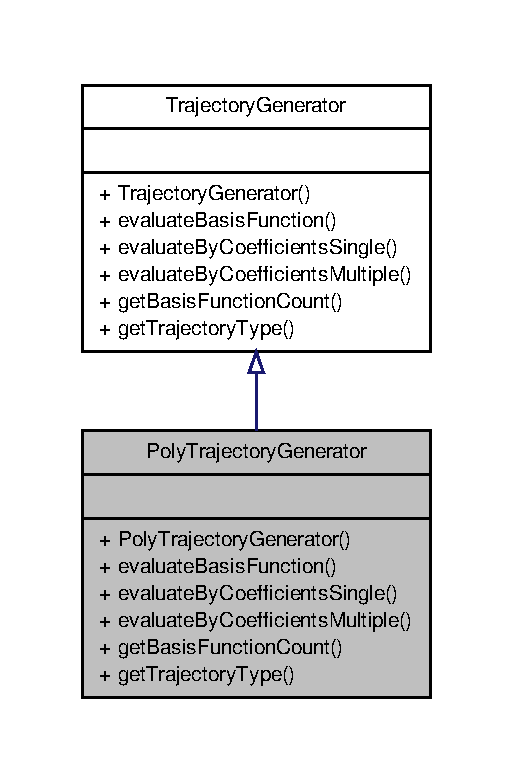
\includegraphics[width=246pt]{classPolyTrajectoryGenerator__inherit__graph}
\end{center}
\end{figure}


\-Collaboration diagram for \-Poly\-Trajectory\-Generator\-:\nopagebreak
\begin{figure}[H]
\begin{center}
\leavevmode
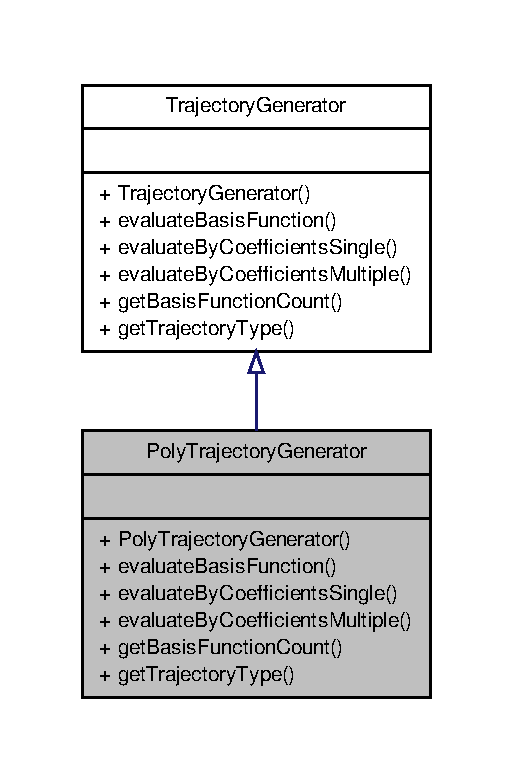
\includegraphics[width=246pt]{classPolyTrajectoryGenerator__coll__graph}
\end{center}
\end{figure}
\subsection*{\-Public \-Member \-Functions}
\begin{DoxyCompactItemize}
\item 
\hyperlink{classPolyTrajectoryGenerator_ae1510d843f50e8e53583d8f5433b16bf}{\-Poly\-Trajectory\-Generator} (int basis\-Function\-Count)
\begin{DoxyCompactList}\small\item\em constructor. the polynomials are defined by giving the degree of the polynomial \end{DoxyCompactList}\item 
double \hyperlink{classPolyTrajectoryGenerator_ade2a3a1dee55b16e56b83ba82f4740db}{evaluate\-Basis\-Function} (double x, int fun)
\begin{DoxyCompactList}\small\item\em evaluates the value of a single basis function \end{DoxyCompactList}\item 
double \hyperlink{classPolyTrajectoryGenerator_ae5b2dbcbd8d3c061cf78a4a48739bfc2}{evaluate\-By\-Coefficients\-Single} (double x, vec coeff)
\begin{DoxyCompactList}\small\item\em evaluates the linear combination of basis functions by defining the coefficients for a single value x \end{DoxyCompactList}\item 
vec \hyperlink{classPolyTrajectoryGenerator_a793a3759c070ae062e21bdc9dd6dc5e9}{evaluate\-By\-Coefficients\-Multiple} (vec x, int sample\-Count, vec coeff)
\begin{DoxyCompactList}\small\item\em performs the same as evaluate\-By\-Coefficients\-Single, but for multiple values of x \end{DoxyCompactList}\item 
int \hyperlink{classPolyTrajectoryGenerator_aaa3de7ffa14a1972dd43136e0ffd96c1}{get\-Basis\-Function\-Count} ()
\begin{DoxyCompactList}\small\item\em returns the number of basis functions \end{DoxyCompactList}\item 
string \hyperlink{classPolyTrajectoryGenerator_afbad1b2268151069d1279ecf734cccb1}{get\-Trajectory\-Type} ()
\begin{DoxyCompactList}\small\item\em returns the name of the basis function system as a string \end{DoxyCompactList}\end{DoxyCompactItemize}


\subsection{\-Detailed \-Description}
\-This class provides simple polynomials as basis functions. f(x) = sum c\-\_\-i x$^\wedge$i 

\subsection{\-Constructor \& \-Destructor \-Documentation}
\hypertarget{classPolyTrajectoryGenerator_ae1510d843f50e8e53583d8f5433b16bf}{\index{\-Poly\-Trajectory\-Generator@{\-Poly\-Trajectory\-Generator}!\-Poly\-Trajectory\-Generator@{\-Poly\-Trajectory\-Generator}}
\index{\-Poly\-Trajectory\-Generator@{\-Poly\-Trajectory\-Generator}!PolyTrajectoryGenerator@{\-Poly\-Trajectory\-Generator}}
\subsubsection[{\-Poly\-Trajectory\-Generator}]{\setlength{\rightskip}{0pt plus 5cm}{\bf \-Poly\-Trajectory\-Generator\-::\-Poly\-Trajectory\-Generator} (
\begin{DoxyParamCaption}
\item[{int}]{basis\-Function\-Count}
\end{DoxyParamCaption}
)}}\label{classPolyTrajectoryGenerator_ae1510d843f50e8e53583d8f5433b16bf}

\begin{DoxyParams}{\-Parameters}
{\em basis\-Function\-Count} & polynomial degree \\
\hline
\end{DoxyParams}


\subsection{\-Member \-Function \-Documentation}
\hypertarget{classPolyTrajectoryGenerator_ade2a3a1dee55b16e56b83ba82f4740db}{\index{\-Poly\-Trajectory\-Generator@{\-Poly\-Trajectory\-Generator}!evaluate\-Basis\-Function@{evaluate\-Basis\-Function}}
\index{evaluate\-Basis\-Function@{evaluate\-Basis\-Function}!PolyTrajectoryGenerator@{\-Poly\-Trajectory\-Generator}}
\subsubsection[{evaluate\-Basis\-Function}]{\setlength{\rightskip}{0pt plus 5cm}double {\bf \-Poly\-Trajectory\-Generator\-::evaluate\-Basis\-Function} (
\begin{DoxyParamCaption}
\item[{double}]{x, }
\item[{int}]{fun}
\end{DoxyParamCaption}
)\hspace{0.3cm}{\ttfamily  \mbox{[}virtual\mbox{]}}}}\label{classPolyTrajectoryGenerator_ade2a3a1dee55b16e56b83ba82f4740db}

\begin{DoxyParams}{\-Parameters}
{\em x} & value, where the basis function should be evaluated \\
\hline
{\em fun} & basis function index that specifies the basis function \\
\hline
\end{DoxyParams}


\-Implements \hyperlink{classTrajectoryGenerator_a2f2305b2cb435b0fa7685937516022e1}{\-Trajectory\-Generator}.

\hypertarget{classPolyTrajectoryGenerator_a793a3759c070ae062e21bdc9dd6dc5e9}{\index{\-Poly\-Trajectory\-Generator@{\-Poly\-Trajectory\-Generator}!evaluate\-By\-Coefficients\-Multiple@{evaluate\-By\-Coefficients\-Multiple}}
\index{evaluate\-By\-Coefficients\-Multiple@{evaluate\-By\-Coefficients\-Multiple}!PolyTrajectoryGenerator@{\-Poly\-Trajectory\-Generator}}
\subsubsection[{evaluate\-By\-Coefficients\-Multiple}]{\setlength{\rightskip}{0pt plus 5cm}vec {\bf \-Poly\-Trajectory\-Generator\-::evaluate\-By\-Coefficients\-Multiple} (
\begin{DoxyParamCaption}
\item[{vec}]{x, }
\item[{int}]{sample\-Count, }
\item[{vec}]{coeff}
\end{DoxyParamCaption}
)\hspace{0.3cm}{\ttfamily  \mbox{[}virtual\mbox{]}}}}\label{classPolyTrajectoryGenerator_a793a3759c070ae062e21bdc9dd6dc5e9}

\begin{DoxyParams}{\-Parameters}
{\em x} & vector of evaluation points \\
\hline
{\em sample\-Count} & size of vector x \\
\hline
{\em coeff} & coefficients that have to be used for computing the linear combination \\
\hline
\end{DoxyParams}


\-Implements \hyperlink{classTrajectoryGenerator_a015de9be72b70ce71675069f4b3361c2}{\-Trajectory\-Generator}.

\hypertarget{classPolyTrajectoryGenerator_ae5b2dbcbd8d3c061cf78a4a48739bfc2}{\index{\-Poly\-Trajectory\-Generator@{\-Poly\-Trajectory\-Generator}!evaluate\-By\-Coefficients\-Single@{evaluate\-By\-Coefficients\-Single}}
\index{evaluate\-By\-Coefficients\-Single@{evaluate\-By\-Coefficients\-Single}!PolyTrajectoryGenerator@{\-Poly\-Trajectory\-Generator}}
\subsubsection[{evaluate\-By\-Coefficients\-Single}]{\setlength{\rightskip}{0pt plus 5cm}double {\bf \-Poly\-Trajectory\-Generator\-::evaluate\-By\-Coefficients\-Single} (
\begin{DoxyParamCaption}
\item[{double}]{x, }
\item[{vec}]{coeff}
\end{DoxyParamCaption}
)\hspace{0.3cm}{\ttfamily  \mbox{[}virtual\mbox{]}}}}\label{classPolyTrajectoryGenerator_ae5b2dbcbd8d3c061cf78a4a48739bfc2}

\begin{DoxyParams}{\-Parameters}
{\em x} & value, where the basis functions should be evaluated \\
\hline
{\em coeff} & coefficients that have to be used for computing the linear combination \\
\hline
\end{DoxyParams}


\-Implements \hyperlink{classTrajectoryGenerator_adcc7ede9c713112796a9fc9f1bf4fec2}{\-Trajectory\-Generator}.

\hypertarget{classPolyTrajectoryGenerator_aaa3de7ffa14a1972dd43136e0ffd96c1}{\index{\-Poly\-Trajectory\-Generator@{\-Poly\-Trajectory\-Generator}!get\-Basis\-Function\-Count@{get\-Basis\-Function\-Count}}
\index{get\-Basis\-Function\-Count@{get\-Basis\-Function\-Count}!PolyTrajectoryGenerator@{\-Poly\-Trajectory\-Generator}}
\subsubsection[{get\-Basis\-Function\-Count}]{\setlength{\rightskip}{0pt plus 5cm}int {\bf \-Poly\-Trajectory\-Generator\-::get\-Basis\-Function\-Count} (
\begin{DoxyParamCaption}
{}
\end{DoxyParamCaption}
)\hspace{0.3cm}{\ttfamily  \mbox{[}virtual\mbox{]}}}}\label{classPolyTrajectoryGenerator_aaa3de7ffa14a1972dd43136e0ffd96c1}


\-Implements \hyperlink{classTrajectoryGenerator_a8d3c339d0c8488873074c8bce918afae}{\-Trajectory\-Generator}.

\hypertarget{classPolyTrajectoryGenerator_afbad1b2268151069d1279ecf734cccb1}{\index{\-Poly\-Trajectory\-Generator@{\-Poly\-Trajectory\-Generator}!get\-Trajectory\-Type@{get\-Trajectory\-Type}}
\index{get\-Trajectory\-Type@{get\-Trajectory\-Type}!PolyTrajectoryGenerator@{\-Poly\-Trajectory\-Generator}}
\subsubsection[{get\-Trajectory\-Type}]{\setlength{\rightskip}{0pt plus 5cm}string {\bf \-Poly\-Trajectory\-Generator\-::get\-Trajectory\-Type} (
\begin{DoxyParamCaption}
{}
\end{DoxyParamCaption}
)\hspace{0.3cm}{\ttfamily  \mbox{[}virtual\mbox{]}}}}\label{classPolyTrajectoryGenerator_afbad1b2268151069d1279ecf734cccb1}


\-Implements \hyperlink{classTrajectoryGenerator_a14e3b583fcee58d393360ef0eb0fb71c}{\-Trajectory\-Generator}.



\-The documentation for this class was generated from the following files\-:\begin{DoxyCompactItemize}
\item 
/home/shangl/data/data\-\_\-synched/studium/informatik/master/master\-\_\-thesis/kukadu\-\_\-framework/thesis/src/trajectory/\hyperlink{PolyTrajectoryGenerator_8h}{\-Poly\-Trajectory\-Generator.\-h}\item 
/home/shangl/data/data\-\_\-synched/studium/informatik/master/master\-\_\-thesis/kukadu\-\_\-framework/thesis/src/trajectory/\hyperlink{PolyTrajectoryGenerator_8cpp}{\-Poly\-Trajectory\-Generator.\-cpp}\end{DoxyCompactItemize}

\hypertarget{classQuadraticKernel}{\section{\-Quadratic\-Kernel \-Class \-Reference}
\label{classQuadraticKernel}\index{\-Quadratic\-Kernel@{\-Quadratic\-Kernel}}
}


\-Implements a quadratic kernel according to the \hyperlink{classGenericKernel}{\-Generic\-Kernel} specifiction.  




{\ttfamily \#include $<$\-Quadratic\-Kernel.\-h$>$}



\-Inheritance diagram for \-Quadratic\-Kernel\-:\nopagebreak
\begin{figure}[H]
\begin{center}
\leavevmode
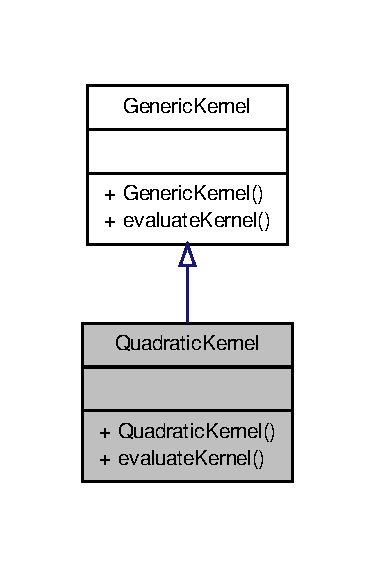
\includegraphics[width=180pt]{classQuadraticKernel__inherit__graph}
\end{center}
\end{figure}


\-Collaboration diagram for \-Quadratic\-Kernel\-:\nopagebreak
\begin{figure}[H]
\begin{center}
\leavevmode
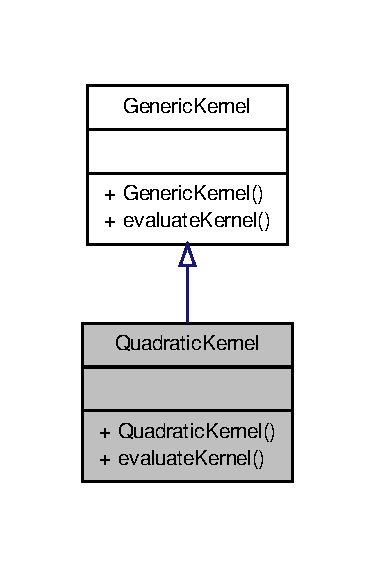
\includegraphics[width=180pt]{classQuadraticKernel__coll__graph}
\end{center}
\end{figure}
\subsection*{\-Public \-Member \-Functions}
\begin{DoxyCompactItemize}
\item 
\hyperlink{classQuadraticKernel_a2121d77dc2d6596c5ddaf41d48497e31}{\-Quadratic\-Kernel} ()
\begin{DoxyCompactList}\small\item\em constructor \end{DoxyCompactList}\item 
double \hyperlink{classQuadraticKernel_a0e7260845bf72f6fb61722cfe7c4b984}{evaluate\-Kernel} (vec q1, vec q2, void $\ast$kernel\-Param)
\begin{DoxyCompactList}\small\item\em computes kernel values with given vectors q1 and q2 and passes a not further specified kernel parameter that can be used by the kernel implementation \end{DoxyCompactList}\end{DoxyCompactItemize}


\subsection{\-Detailed \-Description}
\-This class implements a quadratic kernel given by the function \-K(u) = 15/16 (1 -\/ $|$u$|$$^\wedge$2)$^\wedge$2 

\subsection{\-Constructor \& \-Destructor \-Documentation}
\hypertarget{classQuadraticKernel_a2121d77dc2d6596c5ddaf41d48497e31}{\index{\-Quadratic\-Kernel@{\-Quadratic\-Kernel}!\-Quadratic\-Kernel@{\-Quadratic\-Kernel}}
\index{\-Quadratic\-Kernel@{\-Quadratic\-Kernel}!QuadraticKernel@{\-Quadratic\-Kernel}}
\subsubsection[{\-Quadratic\-Kernel}]{\setlength{\rightskip}{0pt plus 5cm}{\bf \-Quadratic\-Kernel\-::\-Quadratic\-Kernel} (
\begin{DoxyParamCaption}
{}
\end{DoxyParamCaption}
)}}\label{classQuadraticKernel_a2121d77dc2d6596c5ddaf41d48497e31}


\subsection{\-Member \-Function \-Documentation}
\hypertarget{classQuadraticKernel_a0e7260845bf72f6fb61722cfe7c4b984}{\index{\-Quadratic\-Kernel@{\-Quadratic\-Kernel}!evaluate\-Kernel@{evaluate\-Kernel}}
\index{evaluate\-Kernel@{evaluate\-Kernel}!QuadraticKernel@{\-Quadratic\-Kernel}}
\subsubsection[{evaluate\-Kernel}]{\setlength{\rightskip}{0pt plus 5cm}double {\bf \-Quadratic\-Kernel\-::evaluate\-Kernel} (
\begin{DoxyParamCaption}
\item[{vec}]{q1, }
\item[{vec}]{q2, }
\item[{void $\ast$}]{kernel\-Param}
\end{DoxyParamCaption}
)\hspace{0.3cm}{\ttfamily  \mbox{[}virtual\mbox{]}}}}\label{classQuadraticKernel_a0e7260845bf72f6fb61722cfe7c4b984}

\begin{DoxyParams}{\-Parameters}
{\em q1} & vector q1 with \-K = \-K(d(q1, q2)) \\
\hline
{\em q2} & vector q2 with \-K = \-K(d(q1, q2)) \\
\hline
{\em kernel\-Param} & arbitrary kernel parameter \\
\hline
\end{DoxyParams}


\-Implements \hyperlink{classGenericKernel_a5b3ef309f47d56cfcb12d02bf0f0b5c7}{\-Generic\-Kernel}.



\-The documentation for this class was generated from the following files\-:\begin{DoxyCompactItemize}
\item 
/home/shangl/data/data\-\_\-synched/studium/informatik/master/master\-\_\-thesis/kukadu\-\_\-framework/thesis/src/learning/\hyperlink{QuadraticKernel_8h}{\-Quadratic\-Kernel.\-h}\item 
/home/shangl/data/data\-\_\-synched/studium/informatik/master/master\-\_\-thesis/kukadu\-\_\-framework/thesis/src/learning/\hyperlink{QuadraticKernel_8cpp}{\-Quadratic\-Kernel.\-cpp}\end{DoxyCompactItemize}

\hypertarget{classSchunkHand}{\section{\-Schunk\-Hand \-Class \-Reference}
\label{classSchunkHand}\index{\-Schunk\-Hand@{\-Schunk\-Hand}}
}


\-Provides control capabilities for the \-Schunk \-S\-D\-H robotic hand \-Implements the \hyperlink{classGenericHand}{\-Generic\-Hand} interface for the \-Schunk \-S\-D\-H robotic hand. \-Note that using this class the programm has to be executed with root rights.  




{\ttfamily \#include $<$\-Schunk\-Hand.\-h$>$}



\-Inheritance diagram for \-Schunk\-Hand\-:\nopagebreak
\begin{figure}[H]
\begin{center}
\leavevmode
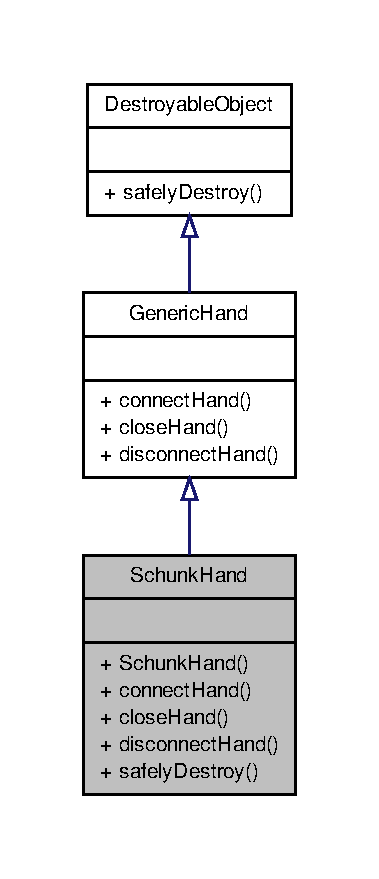
\includegraphics[width=182pt]{classSchunkHand__inherit__graph}
\end{center}
\end{figure}


\-Collaboration diagram for \-Schunk\-Hand\-:\nopagebreak
\begin{figure}[H]
\begin{center}
\leavevmode
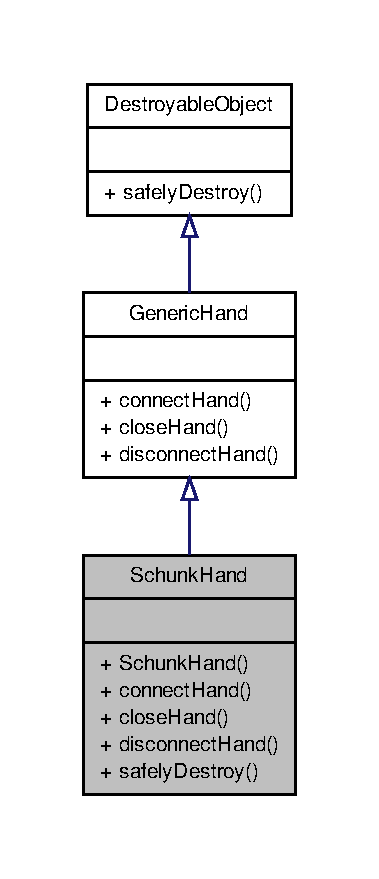
\includegraphics[width=182pt]{classSchunkHand__coll__graph}
\end{center}
\end{figure}
\subsection*{\-Public \-Member \-Functions}
\begin{DoxyCompactItemize}
\item 
\hyperlink{classSchunkHand_ab4c3c0616dffbeb81889dd3cd61df662}{\-Schunk\-Hand} (char $\ast$usb\-Device)
\begin{DoxyCompactList}\small\item\em \hyperlink{classSchunkHand}{\-Schunk\-Hand} constructor taking the connection port name. \end{DoxyCompactList}\item 
void \hyperlink{classSchunkHand_a127722f2f9221a6327cb60a285452d10}{connect\-Hand} ()
\begin{DoxyCompactList}\small\item\em \-Initializes the connection to the hand. \end{DoxyCompactList}\item 
void \hyperlink{classSchunkHand_ad7955193f561aae87b4bf0c9482bc877}{close\-Hand} (double percentage, double velocity)
\begin{DoxyCompactList}\small\item\em \-Opens and closes the hand according to the provided closing percentage and velocity. \end{DoxyCompactList}\item 
void \hyperlink{classSchunkHand_af0c67b101d6cfd19c4758347700c2346}{disconnect\-Hand} ()
\begin{DoxyCompactList}\small\item\em \-Closes connection between host computer and hand. \end{DoxyCompactList}\item 
void \hyperlink{classSchunkHand_a2d1e10b2b14e293edcf84100b07116cc}{safely\-Destroy} ()
\begin{DoxyCompactList}\small\item\em \-Method is called whenever destroy event occurs and ensures safe and clean termination of the programm (e.\-g. stops robot) \end{DoxyCompactList}\end{DoxyCompactItemize}


\subsection{\-Constructor \& \-Destructor \-Documentation}
\hypertarget{classSchunkHand_ab4c3c0616dffbeb81889dd3cd61df662}{\index{\-Schunk\-Hand@{\-Schunk\-Hand}!\-Schunk\-Hand@{\-Schunk\-Hand}}
\index{\-Schunk\-Hand@{\-Schunk\-Hand}!SchunkHand@{\-Schunk\-Hand}}
\subsubsection[{\-Schunk\-Hand}]{\setlength{\rightskip}{0pt plus 5cm}{\bf \-Schunk\-Hand\-::\-Schunk\-Hand} (
\begin{DoxyParamCaption}
\item[{char $\ast$}]{usb\-Device}
\end{DoxyParamCaption}
)}}\label{classSchunkHand_ab4c3c0616dffbeb81889dd3cd61df662}

\begin{DoxyParams}{\-Parameters}
{\em usb\-Device} & usb port name (e.\-g. \char`\"{}/dev/tty\-U\-S\-B0\char`\"{}) \\
\hline
\end{DoxyParams}


\subsection{\-Member \-Function \-Documentation}
\hypertarget{classSchunkHand_ad7955193f561aae87b4bf0c9482bc877}{\index{\-Schunk\-Hand@{\-Schunk\-Hand}!close\-Hand@{close\-Hand}}
\index{close\-Hand@{close\-Hand}!SchunkHand@{\-Schunk\-Hand}}
\subsubsection[{close\-Hand}]{\setlength{\rightskip}{0pt plus 5cm}void {\bf \-Schunk\-Hand\-::close\-Hand} (
\begin{DoxyParamCaption}
\item[{double}]{percentage, }
\item[{double}]{velocity}
\end{DoxyParamCaption}
)\hspace{0.3cm}{\ttfamily  \mbox{[}virtual\mbox{]}}}}\label{classSchunkHand_ad7955193f561aae87b4bf0c9482bc877}

\begin{DoxyParams}{\-Parameters}
{\em percentage} & closing percentage (0.\-0 -\/ hand fully open, 1.\-0 hand fully closed) \\
\hline
{\em velocity} & closing velocity in range between 0 and 1 \\
\hline
\end{DoxyParams}


\-Implements \hyperlink{classGenericHand_a88be8d6c42cfd7b48da1df7da68d2aca}{\-Generic\-Hand}.

\hypertarget{classSchunkHand_a127722f2f9221a6327cb60a285452d10}{\index{\-Schunk\-Hand@{\-Schunk\-Hand}!connect\-Hand@{connect\-Hand}}
\index{connect\-Hand@{connect\-Hand}!SchunkHand@{\-Schunk\-Hand}}
\subsubsection[{connect\-Hand}]{\setlength{\rightskip}{0pt plus 5cm}void {\bf \-Schunk\-Hand\-::connect\-Hand} (
\begin{DoxyParamCaption}
{}
\end{DoxyParamCaption}
)\hspace{0.3cm}{\ttfamily  \mbox{[}virtual\mbox{]}}}}\label{classSchunkHand_a127722f2f9221a6327cb60a285452d10}


\-Implements \hyperlink{classGenericHand_ab8e8610f2ceed53ab3112ceef60e1cd0}{\-Generic\-Hand}.

\hypertarget{classSchunkHand_af0c67b101d6cfd19c4758347700c2346}{\index{\-Schunk\-Hand@{\-Schunk\-Hand}!disconnect\-Hand@{disconnect\-Hand}}
\index{disconnect\-Hand@{disconnect\-Hand}!SchunkHand@{\-Schunk\-Hand}}
\subsubsection[{disconnect\-Hand}]{\setlength{\rightskip}{0pt plus 5cm}void {\bf \-Schunk\-Hand\-::disconnect\-Hand} (
\begin{DoxyParamCaption}
{}
\end{DoxyParamCaption}
)\hspace{0.3cm}{\ttfamily  \mbox{[}virtual\mbox{]}}}}\label{classSchunkHand_af0c67b101d6cfd19c4758347700c2346}


\-Implements \hyperlink{classGenericHand_acb5b9fff34fc22b9cebbc7d927ec4aa6}{\-Generic\-Hand}.

\hypertarget{classSchunkHand_a2d1e10b2b14e293edcf84100b07116cc}{\index{\-Schunk\-Hand@{\-Schunk\-Hand}!safely\-Destroy@{safely\-Destroy}}
\index{safely\-Destroy@{safely\-Destroy}!SchunkHand@{\-Schunk\-Hand}}
\subsubsection[{safely\-Destroy}]{\setlength{\rightskip}{0pt plus 5cm}void {\bf \-Schunk\-Hand\-::safely\-Destroy} (
\begin{DoxyParamCaption}
{}
\end{DoxyParamCaption}
)\hspace{0.3cm}{\ttfamily  \mbox{[}virtual\mbox{]}}}}\label{classSchunkHand_a2d1e10b2b14e293edcf84100b07116cc}


\-Implements \hyperlink{classDestroyableObject_a728d19d81eca540efd68650867f197be}{\-Destroyable\-Object}.



\-The documentation for this class was generated from the following files\-:\begin{DoxyCompactItemize}
\item 
/home/shangl/data/data\-\_\-synched/studium/informatik/master/master\-\_\-thesis/kukadu\-\_\-framework/thesis/src/robot/mounted/\hyperlink{SchunkHand_8h}{\-Schunk\-Hand.\-h}\item 
/home/shangl/data/data\-\_\-synched/studium/informatik/master/master\-\_\-thesis/kukadu\-\_\-framework/thesis/src/robot/mounted/\hyperlink{SchunkHand_8cpp}{\-Schunk\-Hand.\-cpp}\end{DoxyCompactItemize}

\hypertarget{classTerminalCostComputer}{\section{\-Terminal\-Cost\-Computer \-Class \-Reference}
\label{classTerminalCostComputer}\index{\-Terminal\-Cost\-Computer@{\-Terminal\-Cost\-Computer}}
}


\-The \hyperlink{classTerminalCostComputer}{\-Terminal\-Cost\-Computer} implements the \hyperlink{classCostComputer}{\-Cost\-Computer} interface.  




{\ttfamily \#include $<$\-Terminal\-Cost\-Computer.\-h$>$}



\-Inheritance diagram for \-Terminal\-Cost\-Computer\-:\nopagebreak
\begin{figure}[H]
\begin{center}
\leavevmode
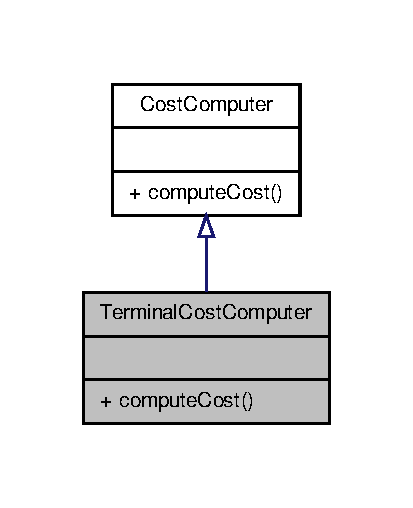
\includegraphics[width=198pt]{classTerminalCostComputer__inherit__graph}
\end{center}
\end{figure}


\-Collaboration diagram for \-Terminal\-Cost\-Computer\-:\nopagebreak
\begin{figure}[H]
\begin{center}
\leavevmode
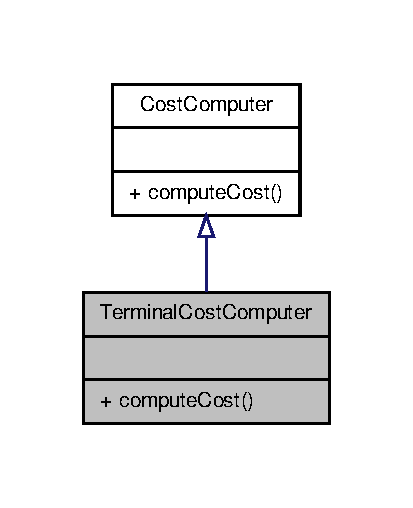
\includegraphics[width=198pt]{classTerminalCostComputer__coll__graph}
\end{center}
\end{figure}
\subsection*{\-Public \-Member \-Functions}
\begin{DoxyCompactItemize}
\item 
double \hyperlink{classTerminalCostComputer_adc77b79cbce50bb7b7b01bf85256d3eb}{compute\-Cost} (t\-\_\-executor\-\_\-res results)
\begin{DoxyCompactList}\small\item\em computes cost for a given dmp execution \end{DoxyCompactList}\end{DoxyCompactItemize}


\subsection{\-Detailed \-Description}
\-This class implements the \hyperlink{classCostComputer}{\-Cost\-Computer} in a simple way. \-The cost of the last rollout is inserted manually by the user to the console. \-This method can be used for very low dimensional reinforcement learning as there a low number of rollouts is needed. 

\subsection{\-Member \-Function \-Documentation}
\hypertarget{classTerminalCostComputer_adc77b79cbce50bb7b7b01bf85256d3eb}{\index{\-Terminal\-Cost\-Computer@{\-Terminal\-Cost\-Computer}!compute\-Cost@{compute\-Cost}}
\index{compute\-Cost@{compute\-Cost}!TerminalCostComputer@{\-Terminal\-Cost\-Computer}}
\subsubsection[{compute\-Cost}]{\setlength{\rightskip}{0pt plus 5cm}double {\bf \-Terminal\-Cost\-Computer\-::compute\-Cost} (
\begin{DoxyParamCaption}
\item[{t\-\_\-executor\-\_\-res}]{results}
\end{DoxyParamCaption}
)\hspace{0.3cm}{\ttfamily  \mbox{[}virtual\mbox{]}}}}\label{classTerminalCostComputer_adc77b79cbce50bb7b7b01bf85256d3eb}

\begin{DoxyParams}{\-Parameters}
{\em results} & measured results of the last dmp execution \\
\hline
\end{DoxyParams}


\-Implements \hyperlink{classCostComputer_a139032631f2d4bd1882d9e5e47960eb0}{\-Cost\-Computer}.



\-The documentation for this class was generated from the following files\-:\begin{DoxyCompactItemize}
\item 
/home/shangl/data/data\-\_\-synched/studium/informatik/master/master\-\_\-thesis/kukadu\-\_\-framework/thesis/src/trajectory/\hyperlink{TerminalCostComputer_8h}{\-Terminal\-Cost\-Computer.\-h}\item 
/home/shangl/data/data\-\_\-synched/studium/informatik/master/master\-\_\-thesis/kukadu\-\_\-framework/thesis/src/trajectory/\hyperlink{TerminalCostComputer_8cpp}{\-Terminal\-Cost\-Computer.\-cpp}\end{DoxyCompactItemize}

\hypertarget{classTrajectoryDMPLearner}{\section{\-Trajectory\-D\-M\-P\-Learner \-Class \-Reference}
\label{classTrajectoryDMPLearner}\index{\-Trajectory\-D\-M\-P\-Learner@{\-Trajectory\-D\-M\-P\-Learner}}
}


\-The \hyperlink{classTrajectoryDMPLearner}{\-Trajectory\-D\-M\-P\-Learner} encapsulates the dmp learning process.  




{\ttfamily \#include $<$\-Trajectory\-D\-M\-P\-Learner.\-h$>$}

\subsection*{\-Public \-Member \-Functions}
\begin{DoxyCompactItemize}
\item 
\hyperlink{classTrajectoryDMPLearner_ae80cd470937dcf56e62e6cbc7d958ecc}{\-Trajectory\-D\-M\-P\-Learner} (dmp\-\_\-base\-\_\-set dmp\-Base, double tau, double az, double bz, double ax, mat joints, int deg\-Freedom)
\begin{DoxyCompactList}\small\item\em constructor \end{DoxyCompactList}\item 
\hyperlink{classTrajectoryDMPLearner_a1bd0b3f7e7661d0675150c574ab443ef}{\-Trajectory\-D\-M\-P\-Learner} (vector$<$ double $>$ mys\-Def, vector$<$ double $>$ sigmas\-Def, double az, double bz, string file, int deg\-Freedom)
\begin{DoxyCompactList}\small\item\em constructor \end{DoxyCompactList}\item 
t\-\_\-learned\-\_\-dmp \hyperlink{classTrajectoryDMPLearner_a92336bee1a8d29ed6975017f5b41b41b}{fit\-Trajectories} ()
\begin{DoxyCompactList}\small\item\em fit the specified trajectories \end{DoxyCompactList}\end{DoxyCompactItemize}


\subsection{\-Detailed \-Description}
\-Dynamic movement primitives can be easily learned by using this class and providing the joint data or a file containing this data. \-Basically this is a helper that enables the programmer to reduce code complexity. 

\subsection{\-Constructor \& \-Destructor \-Documentation}
\hypertarget{classTrajectoryDMPLearner_ae80cd470937dcf56e62e6cbc7d958ecc}{\index{\-Trajectory\-D\-M\-P\-Learner@{\-Trajectory\-D\-M\-P\-Learner}!\-Trajectory\-D\-M\-P\-Learner@{\-Trajectory\-D\-M\-P\-Learner}}
\index{\-Trajectory\-D\-M\-P\-Learner@{\-Trajectory\-D\-M\-P\-Learner}!TrajectoryDMPLearner@{\-Trajectory\-D\-M\-P\-Learner}}
\subsubsection[{\-Trajectory\-D\-M\-P\-Learner}]{\setlength{\rightskip}{0pt plus 5cm}{\bf \-Trajectory\-D\-M\-P\-Learner\-::\-Trajectory\-D\-M\-P\-Learner} (
\begin{DoxyParamCaption}
\item[{dmp\-\_\-base\-\_\-set}]{dmp\-Base, }
\item[{double}]{tau, }
\item[{double}]{az, }
\item[{double}]{bz, }
\item[{double}]{ax, }
\item[{mat}]{joints, }
\item[{int}]{deg\-Freedom}
\end{DoxyParamCaption}
)}}\label{classTrajectoryDMPLearner_ae80cd470937dcf56e62e6cbc7d958ecc}

\begin{DoxyParams}{\-Parameters}
{\em dmp\-Base} & dmp basis function definition \\
\hline
{\em tau} & dmp timing constant \\
\hline
{\em az} & dmp az constant \\
\hline
{\em bz} & dmp bz constant \\
\hline
{\em ax} & dmp ax constant \\
\hline
{\em joints} & measured joints \\
\hline
{\em deg\-Freedom} & robots degrees of freedom \\
\hline
\end{DoxyParams}
\hypertarget{classTrajectoryDMPLearner_a1bd0b3f7e7661d0675150c574ab443ef}{\index{\-Trajectory\-D\-M\-P\-Learner@{\-Trajectory\-D\-M\-P\-Learner}!\-Trajectory\-D\-M\-P\-Learner@{\-Trajectory\-D\-M\-P\-Learner}}
\index{\-Trajectory\-D\-M\-P\-Learner@{\-Trajectory\-D\-M\-P\-Learner}!TrajectoryDMPLearner@{\-Trajectory\-D\-M\-P\-Learner}}
\subsubsection[{\-Trajectory\-D\-M\-P\-Learner}]{\setlength{\rightskip}{0pt plus 5cm}{\bf \-Trajectory\-D\-M\-P\-Learner\-::\-Trajectory\-D\-M\-P\-Learner} (
\begin{DoxyParamCaption}
\item[{vector$<$ double $>$}]{mys\-Def, }
\item[{vector$<$ double $>$}]{sigmas\-Def, }
\item[{double}]{az, }
\item[{double}]{bz, }
\item[{string}]{file, }
\item[{int}]{deg\-Freedom}
\end{DoxyParamCaption}
)}}\label{classTrajectoryDMPLearner_a1bd0b3f7e7661d0675150c574ab443ef}

\begin{DoxyParams}{\-Parameters}
{\em dmp\-Base} & dmp basis function definition \\
\hline
{\em tau} & dmp timing constant \\
\hline
{\em az} & dmp az constant \\
\hline
{\em bz} & dmp bz constant \\
\hline
{\em ax} & dmp ax constant \\
\hline
{\em file} & file containing the measured joints \\
\hline
{\em deg\-Freedom} & robots degrees of freedom \\
\hline
\end{DoxyParams}


\subsection{\-Member \-Function \-Documentation}
\hypertarget{classTrajectoryDMPLearner_a92336bee1a8d29ed6975017f5b41b41b}{\index{\-Trajectory\-D\-M\-P\-Learner@{\-Trajectory\-D\-M\-P\-Learner}!fit\-Trajectories@{fit\-Trajectories}}
\index{fit\-Trajectories@{fit\-Trajectories}!TrajectoryDMPLearner@{\-Trajectory\-D\-M\-P\-Learner}}
\subsubsection[{fit\-Trajectories}]{\setlength{\rightskip}{0pt plus 5cm}t\-\_\-learned\-\_\-dmp {\bf \-Trajectory\-D\-M\-P\-Learner\-::fit\-Trajectories} (
\begin{DoxyParamCaption}
{}
\end{DoxyParamCaption}
)}}\label{classTrajectoryDMPLearner_a92336bee1a8d29ed6975017f5b41b41b}


\-The documentation for this class was generated from the following files\-:\begin{DoxyCompactItemize}
\item 
/home/shangl/data/data\-\_\-synched/studium/informatik/master/master\-\_\-thesis/kukadu\-\_\-framework/thesis/src/trajectory/\hyperlink{TrajectoryDMPLearner_8h}{\-Trajectory\-D\-M\-P\-Learner.\-h}\item 
/home/shangl/data/data\-\_\-synched/studium/informatik/master/master\-\_\-thesis/kukadu\-\_\-framework/thesis/src/trajectory/\hyperlink{TrajectoryDMPLearner_8cpp}{\-Trajectory\-D\-M\-P\-Learner.\-cpp}\end{DoxyCompactItemize}

\hypertarget{classTrajectoryGenerator}{\section{\-Trajectory\-Generator \-Class \-Reference}
\label{classTrajectoryGenerator}\index{\-Trajectory\-Generator@{\-Trajectory\-Generator}}
}


\-The \hyperlink{classTrajectoryGenerator}{\-Trajectory\-Generator} defines an interface to define basis functions for linear regression (see \hyperlink{classGeneralFitter}{\-General\-Fitter})  




{\ttfamily \#include $<$\-Trajectory\-Generator.\-h$>$}



\-Inheritance diagram for \-Trajectory\-Generator\-:\nopagebreak
\begin{figure}[H]
\begin{center}
\leavevmode
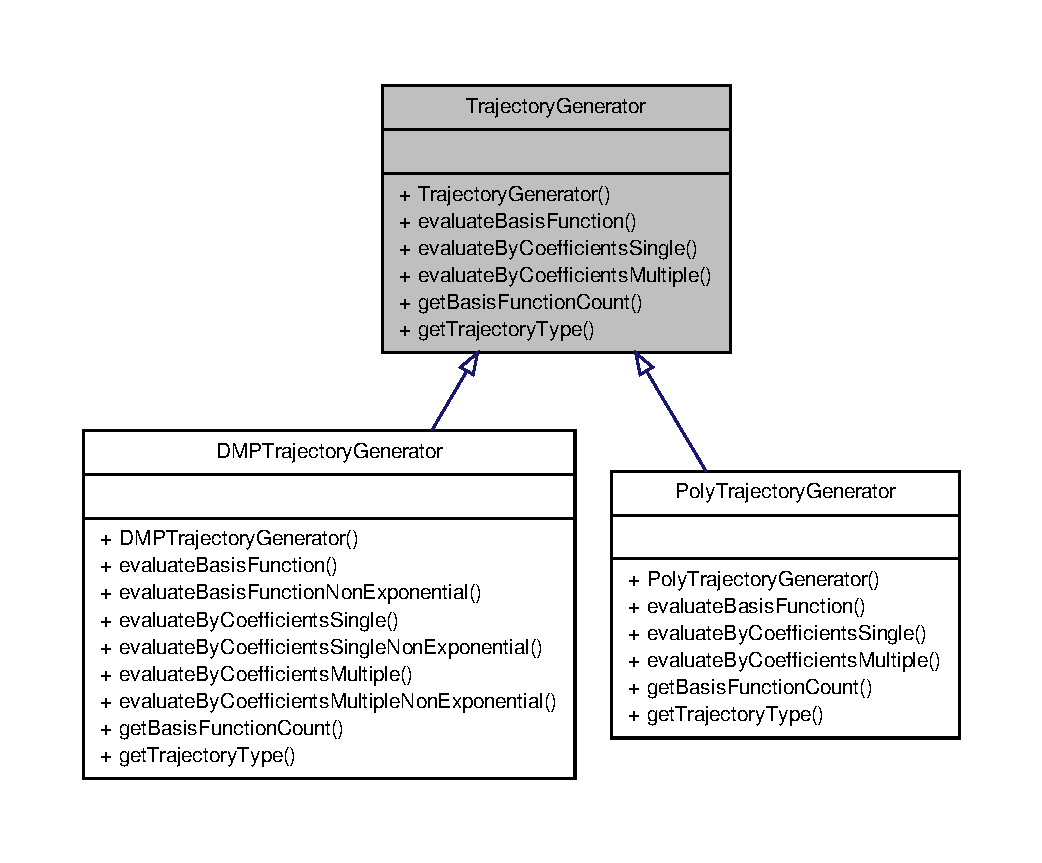
\includegraphics[width=350pt]{classTrajectoryGenerator__inherit__graph}
\end{center}
\end{figure}
\subsection*{\-Public \-Member \-Functions}
\begin{DoxyCompactItemize}
\item 
\hyperlink{classTrajectoryGenerator_af1358bd5e8dad73dbf2b46bf8c0a54a9}{\-Trajectory\-Generator} ()
\begin{DoxyCompactList}\small\item\em constructor \end{DoxyCompactList}\item 
virtual double \hyperlink{classTrajectoryGenerator_a2f2305b2cb435b0fa7685937516022e1}{evaluate\-Basis\-Function} (double x, int fun)=0
\begin{DoxyCompactList}\small\item\em evaluates the value of a single basis function \end{DoxyCompactList}\item 
virtual double \hyperlink{classTrajectoryGenerator_adcc7ede9c713112796a9fc9f1bf4fec2}{evaluate\-By\-Coefficients\-Single} (double x, vec coeff)=0
\begin{DoxyCompactList}\small\item\em evaluates the linear combination of basis functions by defining the coefficients for a single value x \end{DoxyCompactList}\item 
virtual vec \hyperlink{classTrajectoryGenerator_a015de9be72b70ce71675069f4b3361c2}{evaluate\-By\-Coefficients\-Multiple} (vec x, int sample\-Count, vec coeff)=0
\begin{DoxyCompactList}\small\item\em performs the same as evaluate\-By\-Coefficients\-Single, but for multiple values of x \end{DoxyCompactList}\item 
virtual int \hyperlink{classTrajectoryGenerator_a8d3c339d0c8488873074c8bce918afae}{get\-Basis\-Function\-Count} ()=0
\begin{DoxyCompactList}\small\item\em returns the number of basis functions \end{DoxyCompactList}\item 
virtual string \hyperlink{classTrajectoryGenerator_a14e3b583fcee58d393360ef0eb0fb71c}{get\-Trajectory\-Type} ()=0
\begin{DoxyCompactList}\small\item\em returns the name of the basis function system as a string \end{DoxyCompactList}\end{DoxyCompactItemize}


\subsection{\-Detailed \-Description}
\-An implementation of this class has to define an internal index on the basis functions where each basis function value can be computed by setting the basis function index 

\subsection{\-Constructor \& \-Destructor \-Documentation}
\hypertarget{classTrajectoryGenerator_af1358bd5e8dad73dbf2b46bf8c0a54a9}{\index{\-Trajectory\-Generator@{\-Trajectory\-Generator}!\-Trajectory\-Generator@{\-Trajectory\-Generator}}
\index{\-Trajectory\-Generator@{\-Trajectory\-Generator}!TrajectoryGenerator@{\-Trajectory\-Generator}}
\subsubsection[{\-Trajectory\-Generator}]{\setlength{\rightskip}{0pt plus 5cm}{\bf \-Trajectory\-Generator\-::\-Trajectory\-Generator} (
\begin{DoxyParamCaption}
{}
\end{DoxyParamCaption}
)}}\label{classTrajectoryGenerator_af1358bd5e8dad73dbf2b46bf8c0a54a9}


\subsection{\-Member \-Function \-Documentation}
\hypertarget{classTrajectoryGenerator_a2f2305b2cb435b0fa7685937516022e1}{\index{\-Trajectory\-Generator@{\-Trajectory\-Generator}!evaluate\-Basis\-Function@{evaluate\-Basis\-Function}}
\index{evaluate\-Basis\-Function@{evaluate\-Basis\-Function}!TrajectoryGenerator@{\-Trajectory\-Generator}}
\subsubsection[{evaluate\-Basis\-Function}]{\setlength{\rightskip}{0pt plus 5cm}virtual double {\bf \-Trajectory\-Generator\-::evaluate\-Basis\-Function} (
\begin{DoxyParamCaption}
\item[{double}]{x, }
\item[{int}]{fun}
\end{DoxyParamCaption}
)\hspace{0.3cm}{\ttfamily  \mbox{[}pure virtual\mbox{]}}}}\label{classTrajectoryGenerator_a2f2305b2cb435b0fa7685937516022e1}

\begin{DoxyParams}{\-Parameters}
{\em x} & value, where the basis function should be evaluated \\
\hline
{\em fun} & basis function index that specifies the basis function \\
\hline
\end{DoxyParams}


\-Implemented in \hyperlink{classDMPTrajectoryGenerator_a992493451729424e9c6420f112614b25}{\-D\-M\-P\-Trajectory\-Generator}, and \hyperlink{classPolyTrajectoryGenerator_ade2a3a1dee55b16e56b83ba82f4740db}{\-Poly\-Trajectory\-Generator}.

\hypertarget{classTrajectoryGenerator_a015de9be72b70ce71675069f4b3361c2}{\index{\-Trajectory\-Generator@{\-Trajectory\-Generator}!evaluate\-By\-Coefficients\-Multiple@{evaluate\-By\-Coefficients\-Multiple}}
\index{evaluate\-By\-Coefficients\-Multiple@{evaluate\-By\-Coefficients\-Multiple}!TrajectoryGenerator@{\-Trajectory\-Generator}}
\subsubsection[{evaluate\-By\-Coefficients\-Multiple}]{\setlength{\rightskip}{0pt plus 5cm}virtual vec {\bf \-Trajectory\-Generator\-::evaluate\-By\-Coefficients\-Multiple} (
\begin{DoxyParamCaption}
\item[{vec}]{x, }
\item[{int}]{sample\-Count, }
\item[{vec}]{coeff}
\end{DoxyParamCaption}
)\hspace{0.3cm}{\ttfamily  \mbox{[}pure virtual\mbox{]}}}}\label{classTrajectoryGenerator_a015de9be72b70ce71675069f4b3361c2}

\begin{DoxyParams}{\-Parameters}
{\em x} & vector of evaluation points \\
\hline
{\em sample\-Count} & size of vector x \\
\hline
{\em coeff} & coefficients that have to be used for computing the linear combination \\
\hline
\end{DoxyParams}


\-Implemented in \hyperlink{classDMPTrajectoryGenerator_abd9752e2ff28ad3f2e92b333d3d59d9b}{\-D\-M\-P\-Trajectory\-Generator}, and \hyperlink{classPolyTrajectoryGenerator_a793a3759c070ae062e21bdc9dd6dc5e9}{\-Poly\-Trajectory\-Generator}.

\hypertarget{classTrajectoryGenerator_adcc7ede9c713112796a9fc9f1bf4fec2}{\index{\-Trajectory\-Generator@{\-Trajectory\-Generator}!evaluate\-By\-Coefficients\-Single@{evaluate\-By\-Coefficients\-Single}}
\index{evaluate\-By\-Coefficients\-Single@{evaluate\-By\-Coefficients\-Single}!TrajectoryGenerator@{\-Trajectory\-Generator}}
\subsubsection[{evaluate\-By\-Coefficients\-Single}]{\setlength{\rightskip}{0pt plus 5cm}virtual double {\bf \-Trajectory\-Generator\-::evaluate\-By\-Coefficients\-Single} (
\begin{DoxyParamCaption}
\item[{double}]{x, }
\item[{vec}]{coeff}
\end{DoxyParamCaption}
)\hspace{0.3cm}{\ttfamily  \mbox{[}pure virtual\mbox{]}}}}\label{classTrajectoryGenerator_adcc7ede9c713112796a9fc9f1bf4fec2}

\begin{DoxyParams}{\-Parameters}
{\em x} & value, where the basis functions should be evaluated \\
\hline
{\em coeff} & coefficients that have to be used for computing the linear combination \\
\hline
\end{DoxyParams}


\-Implemented in \hyperlink{classDMPTrajectoryGenerator_ad5937ddc13203ab6b11e5366a0c9b57d}{\-D\-M\-P\-Trajectory\-Generator}, and \hyperlink{classPolyTrajectoryGenerator_ae5b2dbcbd8d3c061cf78a4a48739bfc2}{\-Poly\-Trajectory\-Generator}.

\hypertarget{classTrajectoryGenerator_a8d3c339d0c8488873074c8bce918afae}{\index{\-Trajectory\-Generator@{\-Trajectory\-Generator}!get\-Basis\-Function\-Count@{get\-Basis\-Function\-Count}}
\index{get\-Basis\-Function\-Count@{get\-Basis\-Function\-Count}!TrajectoryGenerator@{\-Trajectory\-Generator}}
\subsubsection[{get\-Basis\-Function\-Count}]{\setlength{\rightskip}{0pt plus 5cm}virtual int {\bf \-Trajectory\-Generator\-::get\-Basis\-Function\-Count} (
\begin{DoxyParamCaption}
{}
\end{DoxyParamCaption}
)\hspace{0.3cm}{\ttfamily  \mbox{[}pure virtual\mbox{]}}}}\label{classTrajectoryGenerator_a8d3c339d0c8488873074c8bce918afae}


\-Implemented in \hyperlink{classDMPTrajectoryGenerator_add61de058ac17ce262236066a22bb2d6}{\-D\-M\-P\-Trajectory\-Generator}, and \hyperlink{classPolyTrajectoryGenerator_aaa3de7ffa14a1972dd43136e0ffd96c1}{\-Poly\-Trajectory\-Generator}.

\hypertarget{classTrajectoryGenerator_a14e3b583fcee58d393360ef0eb0fb71c}{\index{\-Trajectory\-Generator@{\-Trajectory\-Generator}!get\-Trajectory\-Type@{get\-Trajectory\-Type}}
\index{get\-Trajectory\-Type@{get\-Trajectory\-Type}!TrajectoryGenerator@{\-Trajectory\-Generator}}
\subsubsection[{get\-Trajectory\-Type}]{\setlength{\rightskip}{0pt plus 5cm}virtual string {\bf \-Trajectory\-Generator\-::get\-Trajectory\-Type} (
\begin{DoxyParamCaption}
{}
\end{DoxyParamCaption}
)\hspace{0.3cm}{\ttfamily  \mbox{[}pure virtual\mbox{]}}}}\label{classTrajectoryGenerator_a14e3b583fcee58d393360ef0eb0fb71c}


\-Implemented in \hyperlink{classDMPTrajectoryGenerator_a69dffc9351054b936ddb9285b4065b3d}{\-D\-M\-P\-Trajectory\-Generator}, and \hyperlink{classPolyTrajectoryGenerator_afbad1b2268151069d1279ecf734cccb1}{\-Poly\-Trajectory\-Generator}.



\-The documentation for this class was generated from the following files\-:\begin{DoxyCompactItemize}
\item 
/home/shangl/data/data\-\_\-synched/studium/informatik/master/master\-\_\-thesis/kukadu\-\_\-framework/thesis/src/trajectory/\hyperlink{TrajectoryGenerator_8h}{\-Trajectory\-Generator.\-h}\item 
/home/shangl/data/data\-\_\-synched/studium/informatik/master/master\-\_\-thesis/kukadu\-\_\-framework/thesis/src/trajectory/\hyperlink{TrajectoryGenerator_8cpp}{\-Trajectory\-Generator.\-cpp}\end{DoxyCompactItemize}

\hypertarget{classTricubeKernel}{\section{\-Tricube\-Kernel \-Class \-Reference}
\label{classTricubeKernel}\index{\-Tricube\-Kernel@{\-Tricube\-Kernel}}
}


\-Implements a tricube kernel according to the \hyperlink{classGenericKernel}{\-Generic\-Kernel} specifiction.  




{\ttfamily \#include $<$\-Tricube\-Kernel.\-h$>$}



\-Inheritance diagram for \-Tricube\-Kernel\-:\nopagebreak
\begin{figure}[H]
\begin{center}
\leavevmode
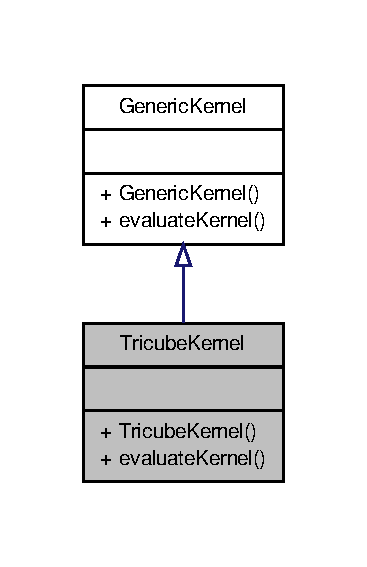
\includegraphics[width=176pt]{classTricubeKernel__inherit__graph}
\end{center}
\end{figure}


\-Collaboration diagram for \-Tricube\-Kernel\-:\nopagebreak
\begin{figure}[H]
\begin{center}
\leavevmode
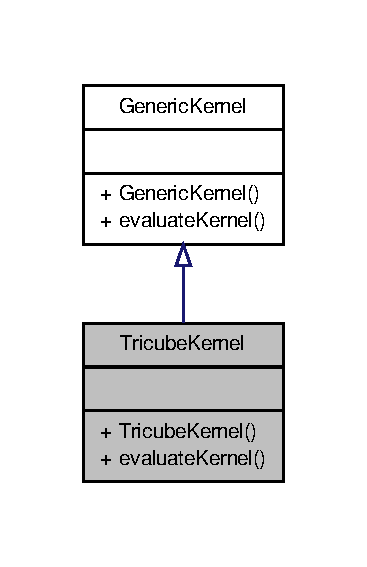
\includegraphics[width=176pt]{classTricubeKernel__coll__graph}
\end{center}
\end{figure}
\subsection*{\-Public \-Member \-Functions}
\begin{DoxyCompactItemize}
\item 
\hyperlink{classTricubeKernel_a31cf424511dc7380148790498be9f3a3}{\-Tricube\-Kernel} ()
\begin{DoxyCompactList}\small\item\em constructor \end{DoxyCompactList}\item 
double \hyperlink{classTricubeKernel_a53a425369baf0bb3e556a08a024baf5c}{evaluate\-Kernel} (vec q1, vec q2, void $\ast$kernel\-Param)
\begin{DoxyCompactList}\small\item\em computes kernel values with given vectors q1 and q2 and passes a not further specified kernel parameter that can be used by the kernel implementation \end{DoxyCompactList}\end{DoxyCompactItemize}


\subsection{\-Detailed \-Description}
\-This class implements a tricube kernel given by the function \-K(u) = 70/81 (1 -\/ $|$u$|$$^\wedge$3)$^\wedge$3 

\subsection{\-Constructor \& \-Destructor \-Documentation}
\hypertarget{classTricubeKernel_a31cf424511dc7380148790498be9f3a3}{\index{\-Tricube\-Kernel@{\-Tricube\-Kernel}!\-Tricube\-Kernel@{\-Tricube\-Kernel}}
\index{\-Tricube\-Kernel@{\-Tricube\-Kernel}!TricubeKernel@{\-Tricube\-Kernel}}
\subsubsection[{\-Tricube\-Kernel}]{\setlength{\rightskip}{0pt plus 5cm}{\bf \-Tricube\-Kernel\-::\-Tricube\-Kernel} (
\begin{DoxyParamCaption}
{}
\end{DoxyParamCaption}
)}}\label{classTricubeKernel_a31cf424511dc7380148790498be9f3a3}


\subsection{\-Member \-Function \-Documentation}
\hypertarget{classTricubeKernel_a53a425369baf0bb3e556a08a024baf5c}{\index{\-Tricube\-Kernel@{\-Tricube\-Kernel}!evaluate\-Kernel@{evaluate\-Kernel}}
\index{evaluate\-Kernel@{evaluate\-Kernel}!TricubeKernel@{\-Tricube\-Kernel}}
\subsubsection[{evaluate\-Kernel}]{\setlength{\rightskip}{0pt plus 5cm}double {\bf \-Tricube\-Kernel\-::evaluate\-Kernel} (
\begin{DoxyParamCaption}
\item[{vec}]{q1, }
\item[{vec}]{q2, }
\item[{void $\ast$}]{kernel\-Param}
\end{DoxyParamCaption}
)\hspace{0.3cm}{\ttfamily  \mbox{[}virtual\mbox{]}}}}\label{classTricubeKernel_a53a425369baf0bb3e556a08a024baf5c}

\begin{DoxyParams}{\-Parameters}
{\em q1} & vector q1 with \-K = \-K(d(q1, q2)) \\
\hline
{\em q2} & vector q2 with \-K = \-K(d(q1, q2)) \\
\hline
{\em kernel\-Param} & arbitrary kernel parameter \\
\hline
\end{DoxyParams}


\-Implements \hyperlink{classGenericKernel_a5b3ef309f47d56cfcb12d02bf0f0b5c7}{\-Generic\-Kernel}.



\-The documentation for this class was generated from the following files\-:\begin{DoxyCompactItemize}
\item 
/home/shangl/data/data\-\_\-synched/studium/informatik/master/master\-\_\-thesis/kukadu\-\_\-framework/thesis/src/learning/\hyperlink{TricubeKernel_8h}{\-Tricube\-Kernel.\-h}\item 
/home/shangl/data/data\-\_\-synched/studium/informatik/master/master\-\_\-thesis/kukadu\-\_\-framework/thesis/src/learning/\hyperlink{TricubeKernel_8cpp}{\-Tricube\-Kernel.\-cpp}\end{DoxyCompactItemize}

\chapter{\-File \-Documentation}
\hypertarget{GaussianKernel_8cpp}{\section{/home/shangl/data/data\-\_\-synched/studium/informatik/master/master\-\_\-thesis/kukadu\-\_\-framework/thesis/src/learning/\-Gaussian\-Kernel.cpp \-File \-Reference}
\label{GaussianKernel_8cpp}\index{/home/shangl/data/data\-\_\-synched/studium/informatik/master/master\-\_\-thesis/kukadu\-\_\-framework/thesis/src/learning/\-Gaussian\-Kernel.\-cpp@{/home/shangl/data/data\-\_\-synched/studium/informatik/master/master\-\_\-thesis/kukadu\-\_\-framework/thesis/src/learning/\-Gaussian\-Kernel.\-cpp}}
}
{\ttfamily \#include \char`\"{}\-Gaussian\-Kernel.\-h\char`\"{}}\*
\-Include dependency graph for \-Gaussian\-Kernel.\-cpp\-:\nopagebreak
\begin{figure}[H]
\begin{center}
\leavevmode
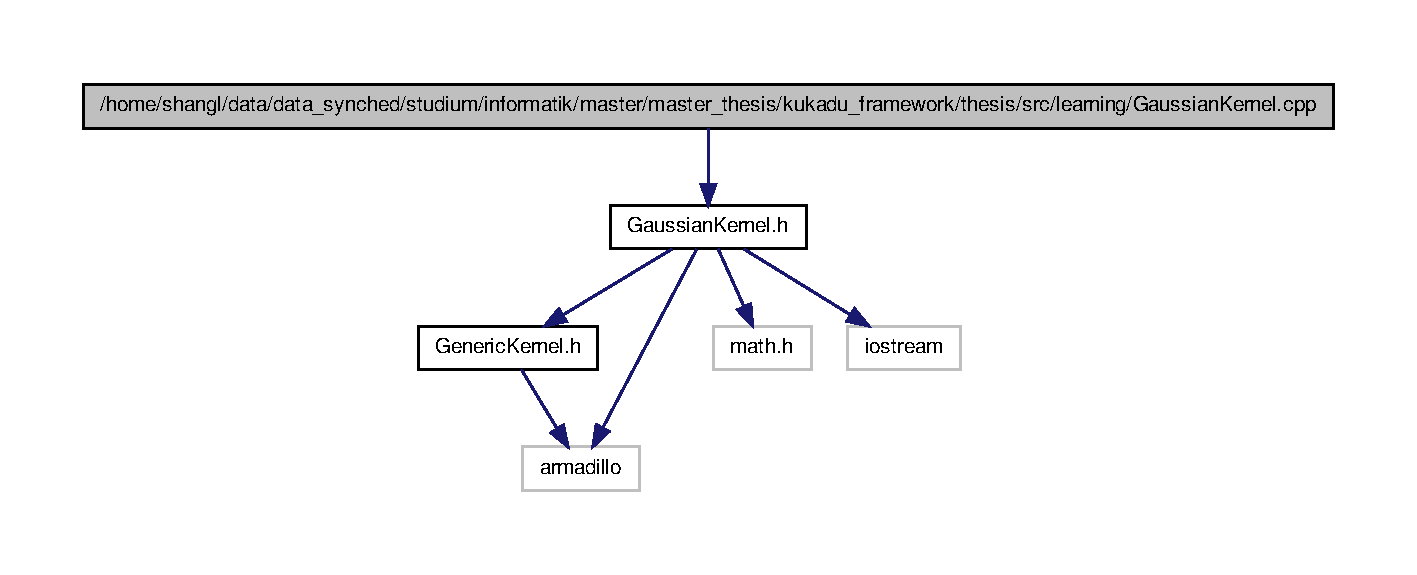
\includegraphics[width=350pt]{GaussianKernel_8cpp__incl}
\end{center}
\end{figure}

\hypertarget{GaussianKernel_8h}{\section{/home/shangl/data/data\-\_\-synched/studium/informatik/master/master\-\_\-thesis/kukadu\-\_\-framework/thesis/src/learning/\-Gaussian\-Kernel.h \-File \-Reference}
\label{GaussianKernel_8h}\index{/home/shangl/data/data\-\_\-synched/studium/informatik/master/master\-\_\-thesis/kukadu\-\_\-framework/thesis/src/learning/\-Gaussian\-Kernel.\-h@{/home/shangl/data/data\-\_\-synched/studium/informatik/master/master\-\_\-thesis/kukadu\-\_\-framework/thesis/src/learning/\-Gaussian\-Kernel.\-h}}
}
{\ttfamily \#include \char`\"{}\-Generic\-Kernel.\-h\char`\"{}}\*
{\ttfamily \#include $<$armadillo$>$}\*
{\ttfamily \#include $<$math.\-h$>$}\*
{\ttfamily \#include $<$iostream$>$}\*
\-Include dependency graph for \-Gaussian\-Kernel.\-h\-:\nopagebreak
\begin{figure}[H]
\begin{center}
\leavevmode
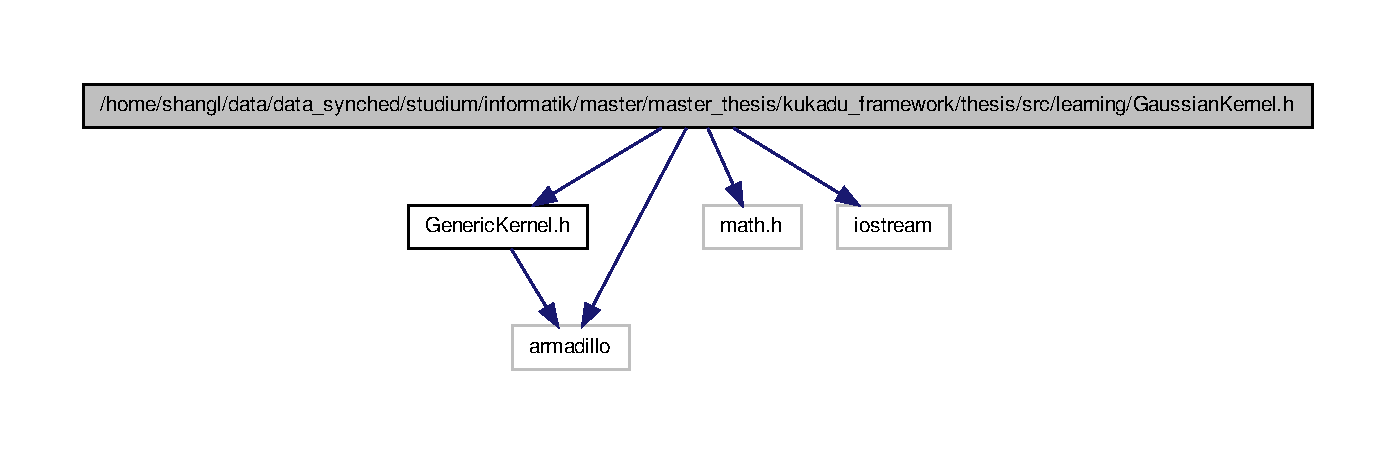
\includegraphics[width=350pt]{GaussianKernel_8h__incl}
\end{center}
\end{figure}
\-This graph shows which files directly or indirectly include this file\-:\nopagebreak
\begin{figure}[H]
\begin{center}
\leavevmode
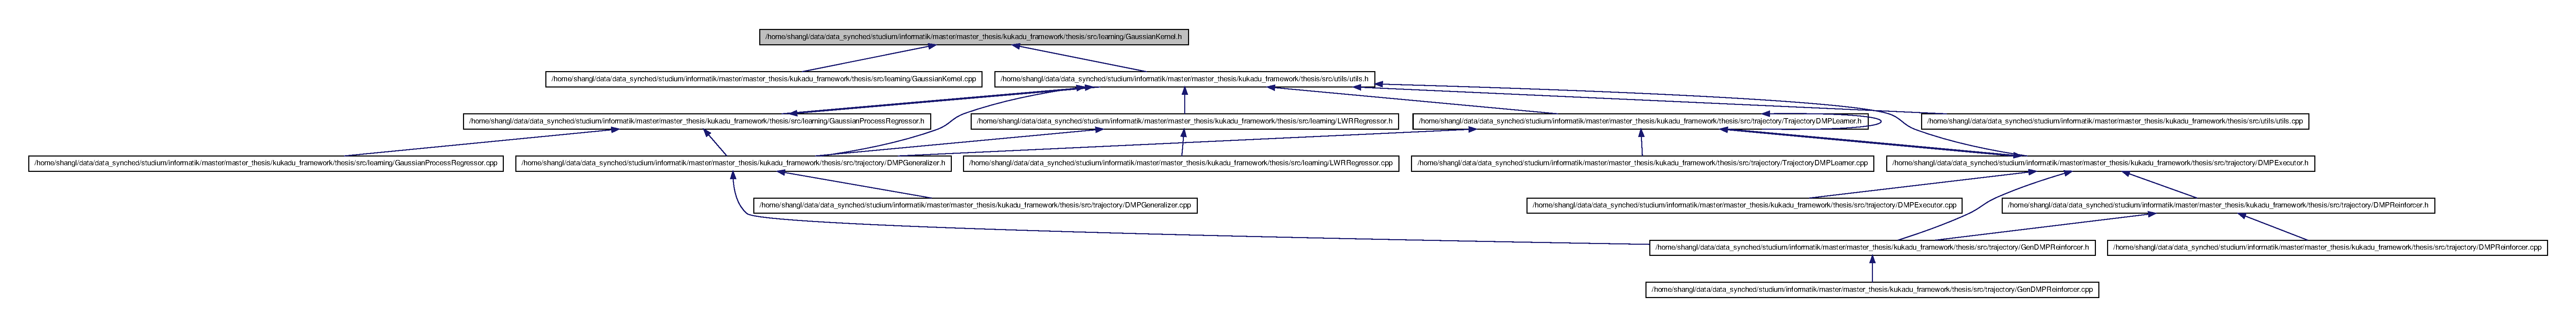
\includegraphics[width=350pt]{GaussianKernel_8h__dep__incl}
\end{center}
\end{figure}
\subsection*{\-Classes}
\begin{DoxyCompactItemize}
\item 
class \hyperlink{classGaussianKernel}{\-Gaussian\-Kernel}
\begin{DoxyCompactList}\small\item\em \-Implements a \-Gaussian kernel according to the \hyperlink{classGenericKernel}{\-Generic\-Kernel} specifiction. \end{DoxyCompactList}\end{DoxyCompactItemize}

\hypertarget{GaussianProcessRegressor_8cpp}{\section{/home/shangl/data/data\-\_\-synched/studium/informatik/master/master\-\_\-thesis/kukadu\-\_\-framework/thesis/src/learning/\-Gaussian\-Process\-Regressor.cpp \-File \-Reference}
\label{GaussianProcessRegressor_8cpp}\index{/home/shangl/data/data\-\_\-synched/studium/informatik/master/master\-\_\-thesis/kukadu\-\_\-framework/thesis/src/learning/\-Gaussian\-Process\-Regressor.\-cpp@{/home/shangl/data/data\-\_\-synched/studium/informatik/master/master\-\_\-thesis/kukadu\-\_\-framework/thesis/src/learning/\-Gaussian\-Process\-Regressor.\-cpp}}
}
{\ttfamily \#include \char`\"{}\-Gaussian\-Process\-Regressor.\-h\char`\"{}}\*
\-Include dependency graph for \-Gaussian\-Process\-Regressor.\-cpp\-:\nopagebreak
\begin{figure}[H]
\begin{center}
\leavevmode
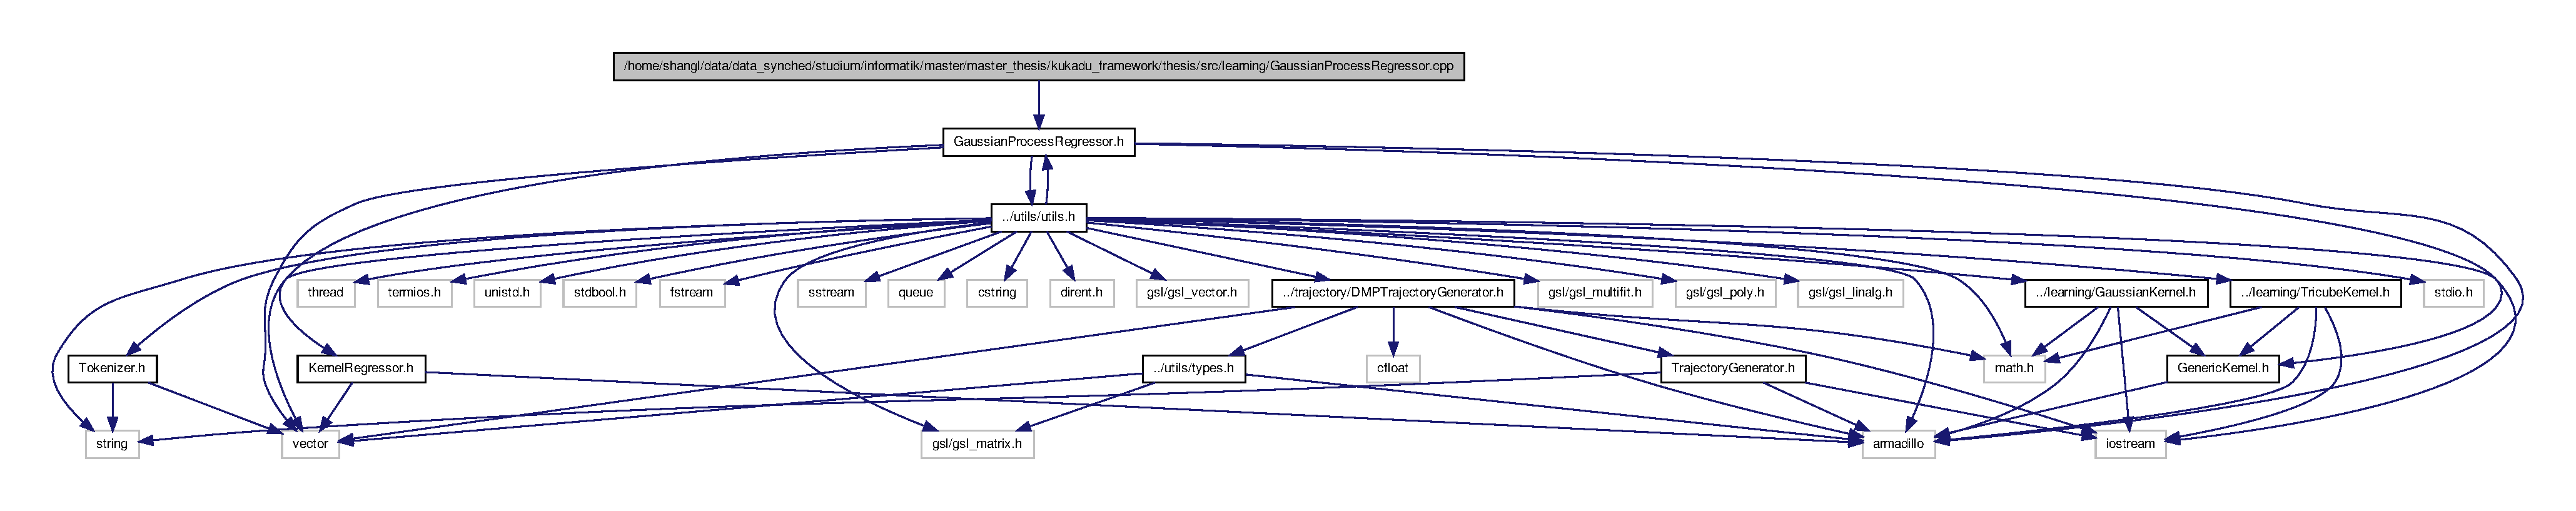
\includegraphics[width=350pt]{GaussianProcessRegressor_8cpp__incl}
\end{center}
\end{figure}

\hypertarget{GaussianProcessRegressor_8h}{\section{/home/shangl/data/data\-\_\-synched/studium/informatik/master/master\-\_\-thesis/kukadu\-\_\-framework/thesis/src/learning/\-Gaussian\-Process\-Regressor.h \-File \-Reference}
\label{GaussianProcessRegressor_8h}\index{/home/shangl/data/data\-\_\-synched/studium/informatik/master/master\-\_\-thesis/kukadu\-\_\-framework/thesis/src/learning/\-Gaussian\-Process\-Regressor.\-h@{/home/shangl/data/data\-\_\-synched/studium/informatik/master/master\-\_\-thesis/kukadu\-\_\-framework/thesis/src/learning/\-Gaussian\-Process\-Regressor.\-h}}
}
{\ttfamily \#include $<$armadillo$>$}\*
{\ttfamily \#include $<$vector$>$}\*
{\ttfamily \#include \char`\"{}\-Kernel\-Regressor.\-h\char`\"{}}\*
{\ttfamily \#include \char`\"{}\-Generic\-Kernel.\-h\char`\"{}}\*
{\ttfamily \#include \char`\"{}../utils/utils.\-h\char`\"{}}\*
\-Include dependency graph for \-Gaussian\-Process\-Regressor.\-h\-:\nopagebreak
\begin{figure}[H]
\begin{center}
\leavevmode
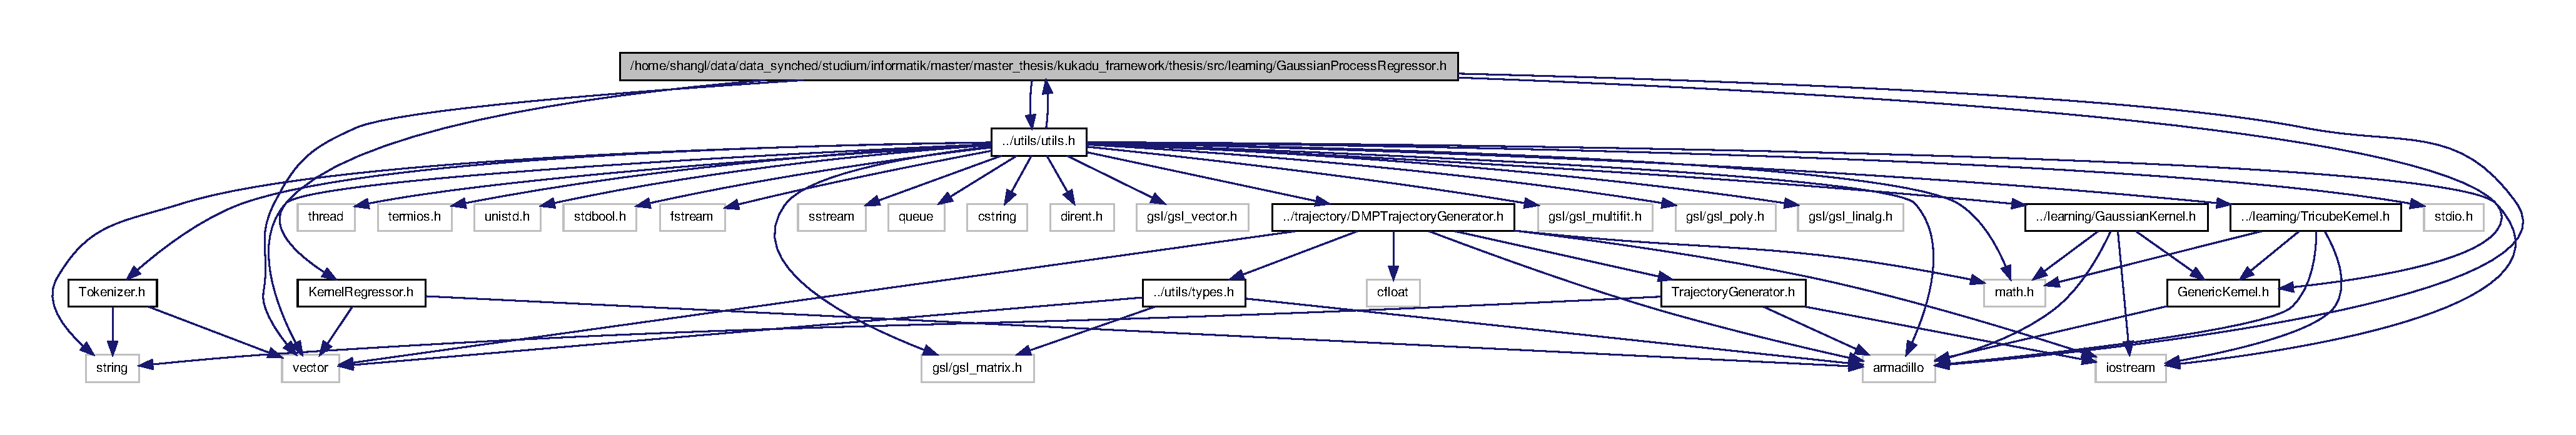
\includegraphics[width=350pt]{GaussianProcessRegressor_8h__incl}
\end{center}
\end{figure}
\-This graph shows which files directly or indirectly include this file\-:\nopagebreak
\begin{figure}[H]
\begin{center}
\leavevmode
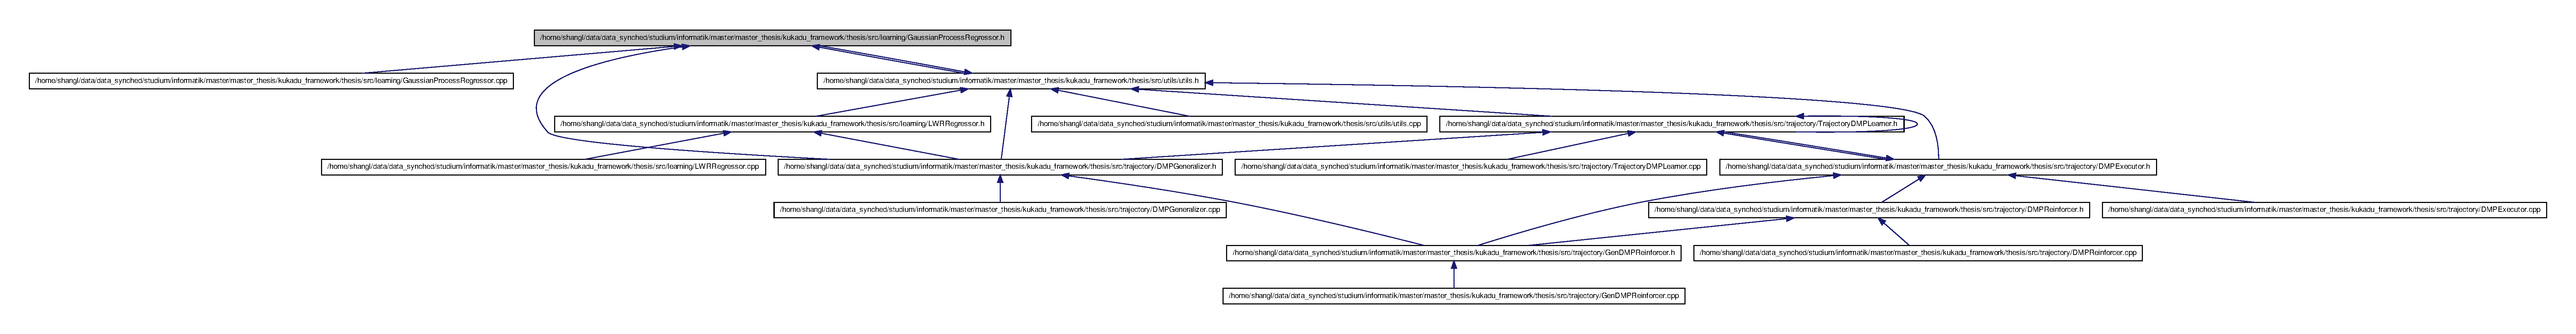
\includegraphics[width=350pt]{GaussianProcessRegressor_8h__dep__incl}
\end{center}
\end{figure}
\subsection*{\-Classes}
\begin{DoxyCompactItemize}
\item 
class \hyperlink{classGaussianProcessRegressor}{\-Gaussian\-Process\-Regressor}
\begin{DoxyCompactList}\small\item\em \-Implements the \-Gaussian process regression method. \end{DoxyCompactList}\end{DoxyCompactItemize}

\hypertarget{GeneralFitter_8cpp}{\section{/home/shangl/data/data\-\_\-synched/studium/informatik/master/master\-\_\-thesis/kukadu\-\_\-framework/thesis/src/learning/\-General\-Fitter.cpp \-File \-Reference}
\label{GeneralFitter_8cpp}\index{/home/shangl/data/data\-\_\-synched/studium/informatik/master/master\-\_\-thesis/kukadu\-\_\-framework/thesis/src/learning/\-General\-Fitter.\-cpp@{/home/shangl/data/data\-\_\-synched/studium/informatik/master/master\-\_\-thesis/kukadu\-\_\-framework/thesis/src/learning/\-General\-Fitter.\-cpp}}
}
{\ttfamily \#include \char`\"{}\-General\-Fitter.\-h\char`\"{}}\*
\-Include dependency graph for \-General\-Fitter.\-cpp\-:\nopagebreak
\begin{figure}[H]
\begin{center}
\leavevmode
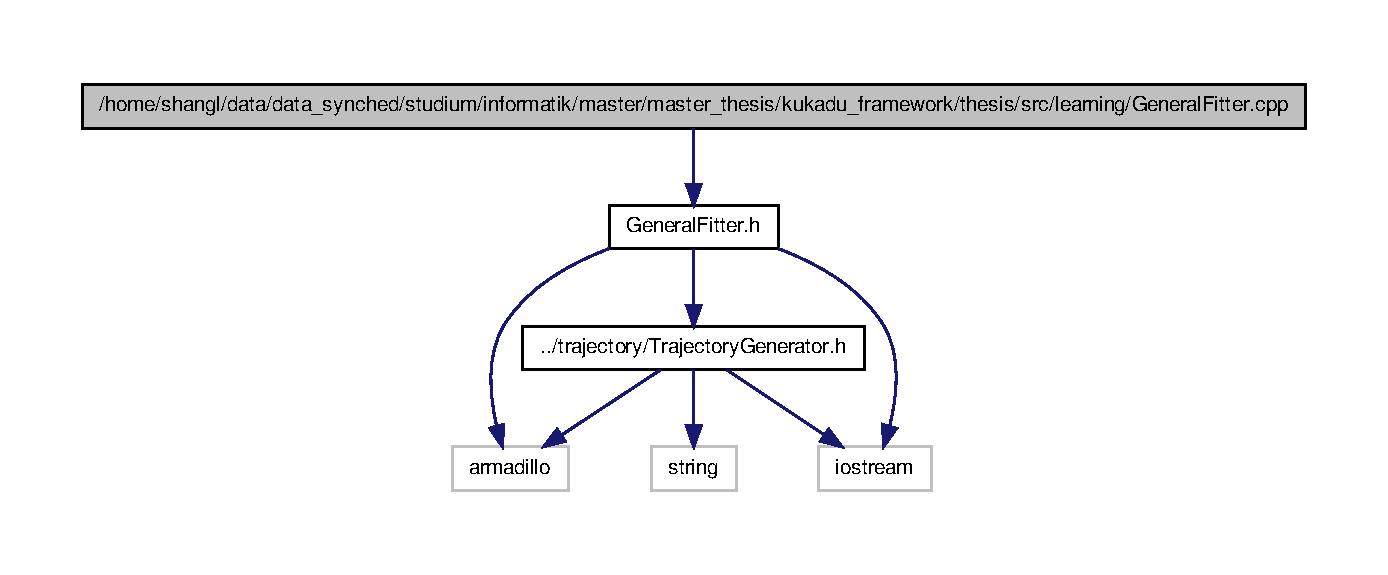
\includegraphics[width=350pt]{GeneralFitter_8cpp__incl}
\end{center}
\end{figure}

\hypertarget{GeneralFitter_8h}{\section{/home/shangl/data/data\-\_\-synched/studium/informatik/master/master\-\_\-thesis/kukadu\-\_\-framework/thesis/src/learning/\-General\-Fitter.h \-File \-Reference}
\label{GeneralFitter_8h}\index{/home/shangl/data/data\-\_\-synched/studium/informatik/master/master\-\_\-thesis/kukadu\-\_\-framework/thesis/src/learning/\-General\-Fitter.\-h@{/home/shangl/data/data\-\_\-synched/studium/informatik/master/master\-\_\-thesis/kukadu\-\_\-framework/thesis/src/learning/\-General\-Fitter.\-h}}
}
{\ttfamily \#include $<$armadillo$>$}\*
{\ttfamily \#include $<$iostream$>$}\*
{\ttfamily \#include \char`\"{}../trajectory/\-Trajectory\-Generator.\-h\char`\"{}}\*
\-Include dependency graph for \-General\-Fitter.\-h\-:\nopagebreak
\begin{figure}[H]
\begin{center}
\leavevmode
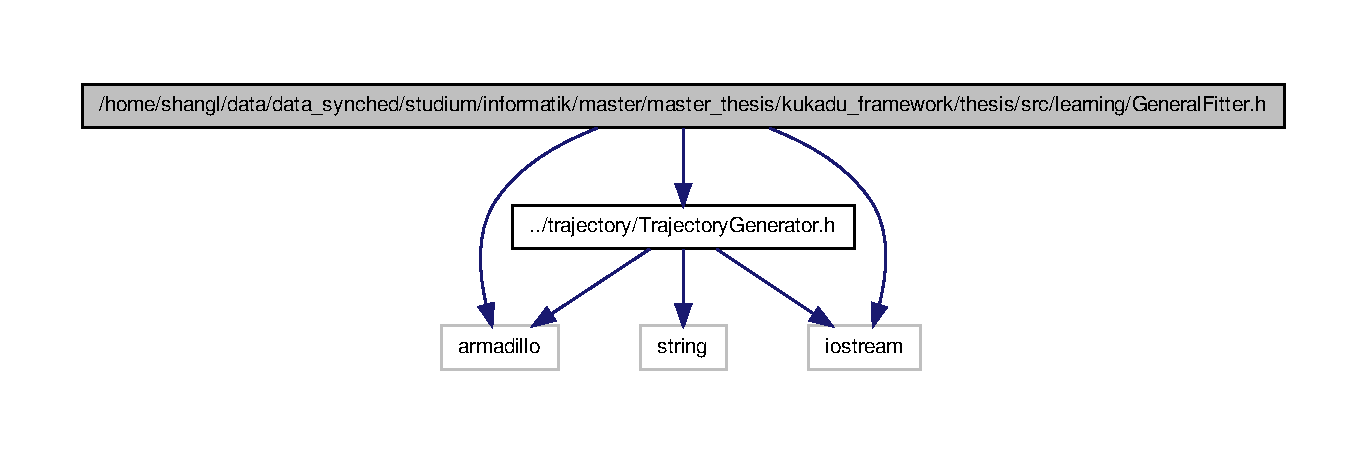
\includegraphics[width=350pt]{GeneralFitter_8h__incl}
\end{center}
\end{figure}
\-This graph shows which files directly or indirectly include this file\-:\nopagebreak
\begin{figure}[H]
\begin{center}
\leavevmode
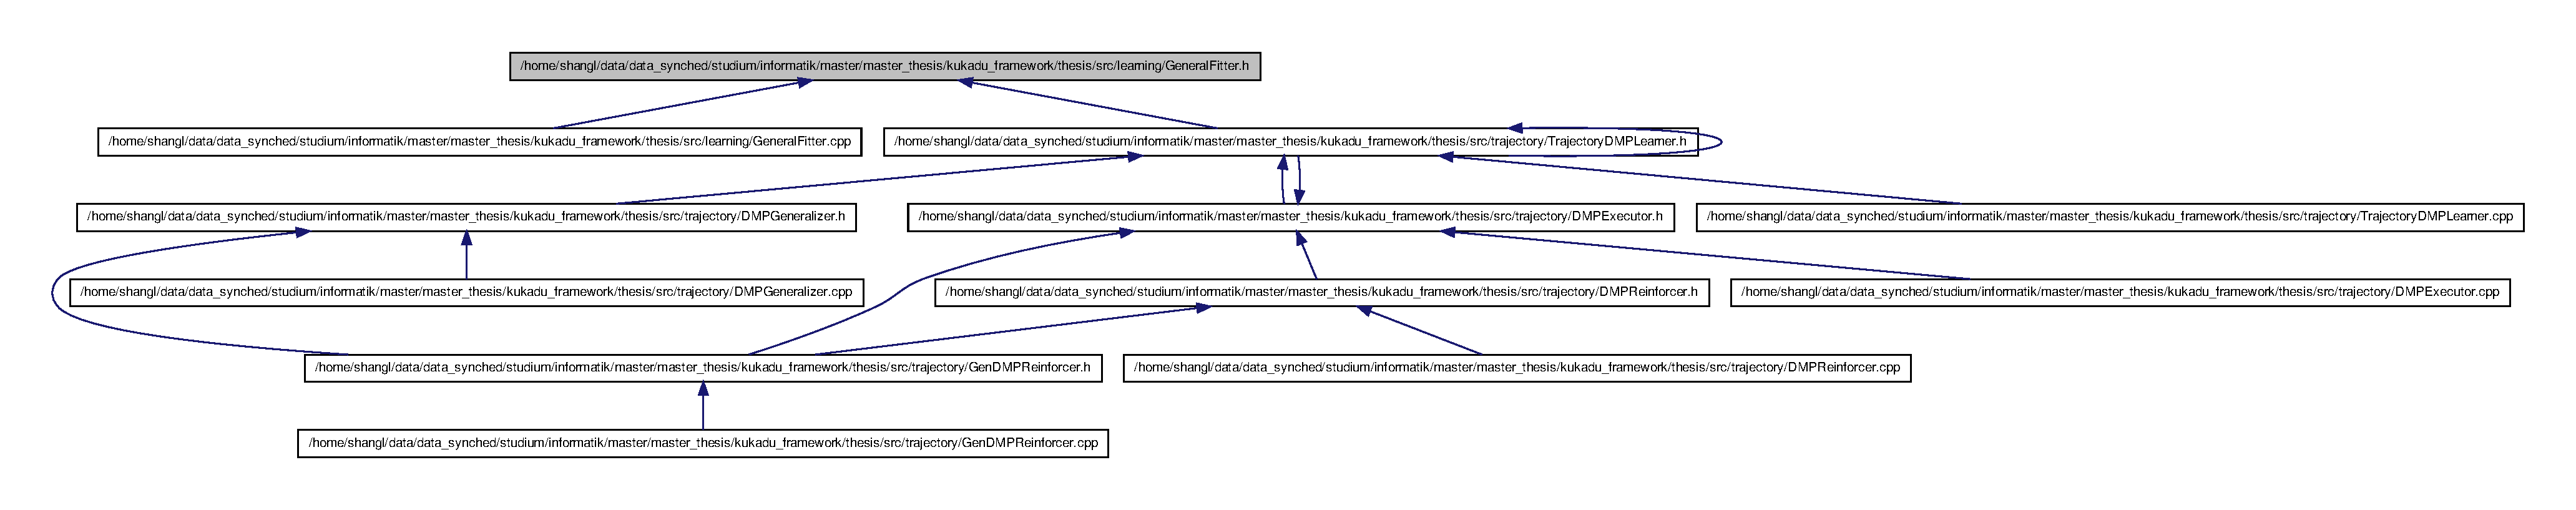
\includegraphics[width=350pt]{GeneralFitter_8h__dep__incl}
\end{center}
\end{figure}
\subsection*{\-Classes}
\begin{DoxyCompactItemize}
\item 
class \hyperlink{classGeneralFitter}{\-General\-Fitter}
\begin{DoxyCompactList}\small\item\em \-Provides the generic part of the linear regression methods. \end{DoxyCompactList}\end{DoxyCompactItemize}

\hypertarget{GenericKernel_8cpp}{\section{/home/shangl/data/data\-\_\-synched/studium/informatik/master/master\-\_\-thesis/kukadu\-\_\-framework/thesis/src/learning/\-Generic\-Kernel.cpp \-File \-Reference}
\label{GenericKernel_8cpp}\index{/home/shangl/data/data\-\_\-synched/studium/informatik/master/master\-\_\-thesis/kukadu\-\_\-framework/thesis/src/learning/\-Generic\-Kernel.\-cpp@{/home/shangl/data/data\-\_\-synched/studium/informatik/master/master\-\_\-thesis/kukadu\-\_\-framework/thesis/src/learning/\-Generic\-Kernel.\-cpp}}
}
{\ttfamily \#include \char`\"{}\-Generic\-Kernel.\-h\char`\"{}}\*
\-Include dependency graph for \-Generic\-Kernel.\-cpp\-:\nopagebreak
\begin{figure}[H]
\begin{center}
\leavevmode
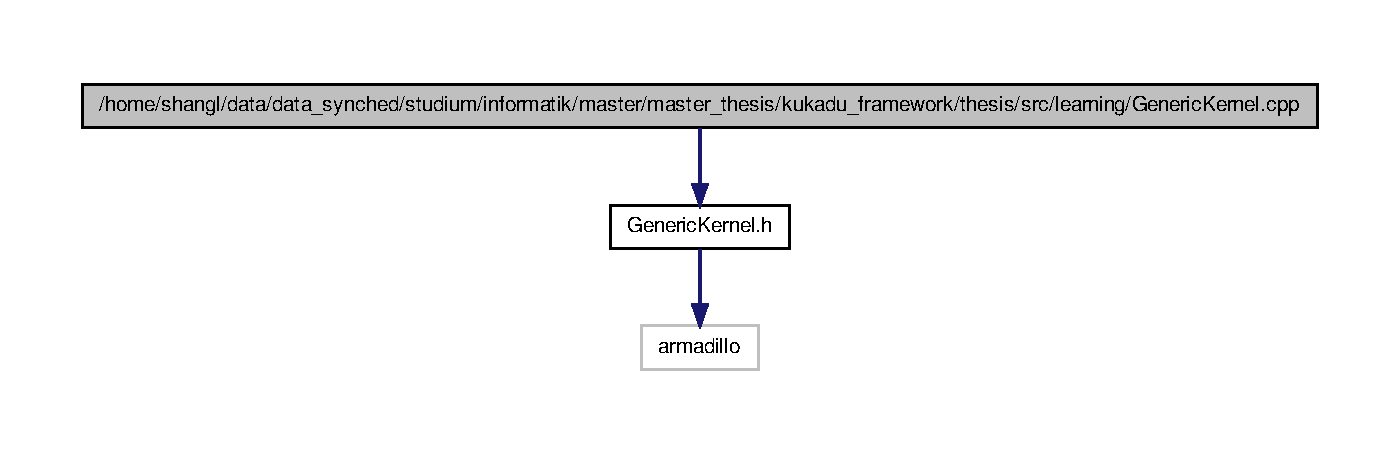
\includegraphics[width=350pt]{GenericKernel_8cpp__incl}
\end{center}
\end{figure}

\hypertarget{GenericKernel_8h}{\section{/home/shangl/data/data\-\_\-synched/studium/informatik/master/master\-\_\-thesis/kukadu\-\_\-framework/thesis/src/learning/\-Generic\-Kernel.h \-File \-Reference}
\label{GenericKernel_8h}\index{/home/shangl/data/data\-\_\-synched/studium/informatik/master/master\-\_\-thesis/kukadu\-\_\-framework/thesis/src/learning/\-Generic\-Kernel.\-h@{/home/shangl/data/data\-\_\-synched/studium/informatik/master/master\-\_\-thesis/kukadu\-\_\-framework/thesis/src/learning/\-Generic\-Kernel.\-h}}
}
{\ttfamily \#include $<$armadillo$>$}\*
\-Include dependency graph for \-Generic\-Kernel.\-h\-:\nopagebreak
\begin{figure}[H]
\begin{center}
\leavevmode
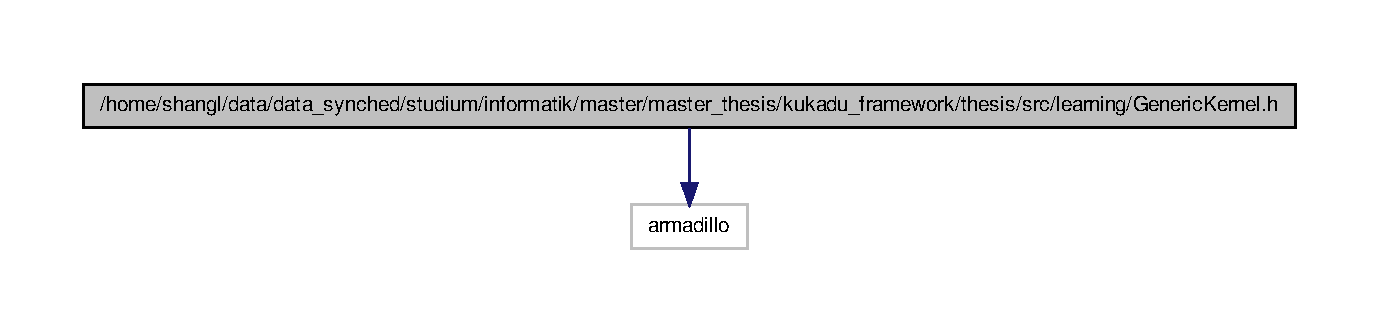
\includegraphics[width=350pt]{GenericKernel_8h__incl}
\end{center}
\end{figure}
\-This graph shows which files directly or indirectly include this file\-:\nopagebreak
\begin{figure}[H]
\begin{center}
\leavevmode
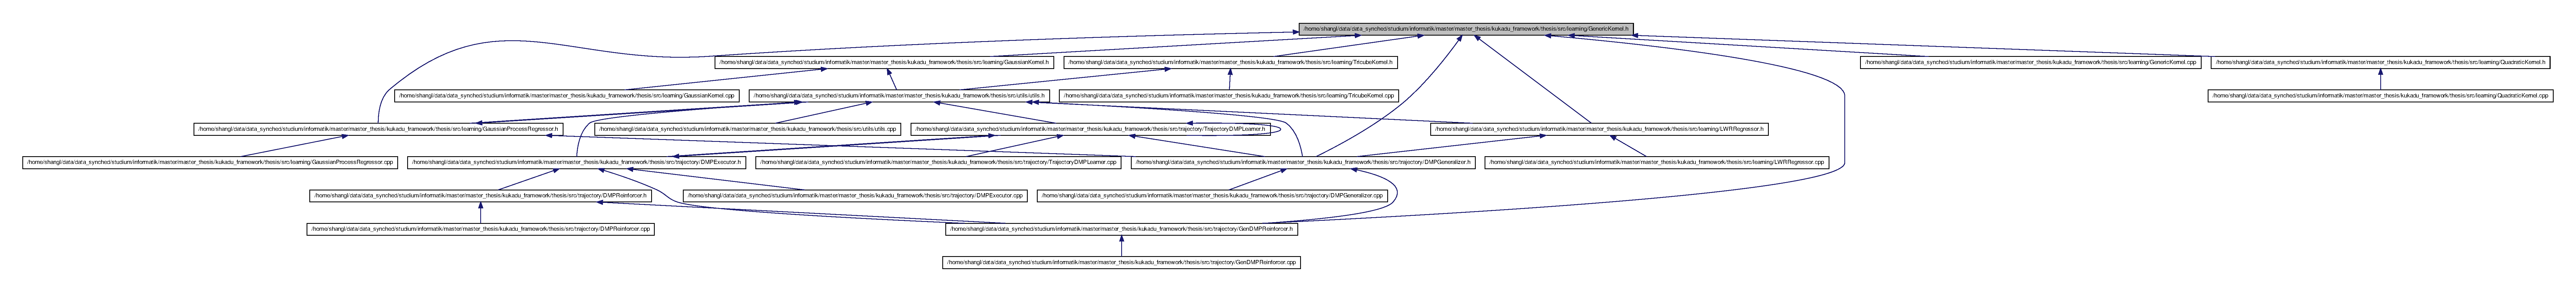
\includegraphics[width=350pt]{GenericKernel_8h__dep__incl}
\end{center}
\end{figure}
\subsection*{\-Classes}
\begin{DoxyCompactItemize}
\item 
class \hyperlink{classGenericKernel}{\-Generic\-Kernel}
\begin{DoxyCompactList}\small\item\em \-Provides an interface for generic kernel functions. \end{DoxyCompactList}\end{DoxyCompactItemize}

\hypertarget{KernelRegressor_8cpp}{\section{/home/shangl/data/data\-\_\-synched/studium/informatik/master/master\-\_\-thesis/kukadu\-\_\-framework/thesis/src/learning/\-Kernel\-Regressor.cpp \-File \-Reference}
\label{KernelRegressor_8cpp}\index{/home/shangl/data/data\-\_\-synched/studium/informatik/master/master\-\_\-thesis/kukadu\-\_\-framework/thesis/src/learning/\-Kernel\-Regressor.\-cpp@{/home/shangl/data/data\-\_\-synched/studium/informatik/master/master\-\_\-thesis/kukadu\-\_\-framework/thesis/src/learning/\-Kernel\-Regressor.\-cpp}}
}
{\ttfamily \#include \char`\"{}\-Kernel\-Regressor.\-h\char`\"{}}\*
\-Include dependency graph for \-Kernel\-Regressor.\-cpp\-:\nopagebreak
\begin{figure}[H]
\begin{center}
\leavevmode
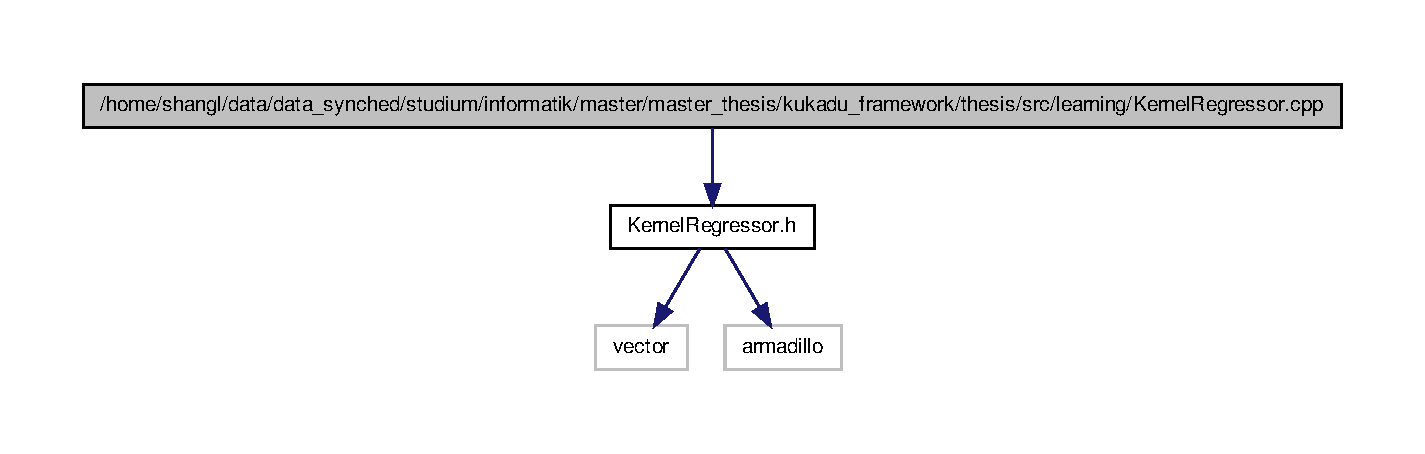
\includegraphics[width=350pt]{KernelRegressor_8cpp__incl}
\end{center}
\end{figure}

\hypertarget{KernelRegressor_8h}{\section{/home/shangl/data/data\-\_\-synched/studium/informatik/master/master\-\_\-thesis/kukadu\-\_\-framework/thesis/src/learning/\-Kernel\-Regressor.h \-File \-Reference}
\label{KernelRegressor_8h}\index{/home/shangl/data/data\-\_\-synched/studium/informatik/master/master\-\_\-thesis/kukadu\-\_\-framework/thesis/src/learning/\-Kernel\-Regressor.\-h@{/home/shangl/data/data\-\_\-synched/studium/informatik/master/master\-\_\-thesis/kukadu\-\_\-framework/thesis/src/learning/\-Kernel\-Regressor.\-h}}
}
{\ttfamily \#include $<$vector$>$}\*
{\ttfamily \#include $<$armadillo$>$}\*
\-Include dependency graph for \-Kernel\-Regressor.\-h\-:\nopagebreak
\begin{figure}[H]
\begin{center}
\leavevmode
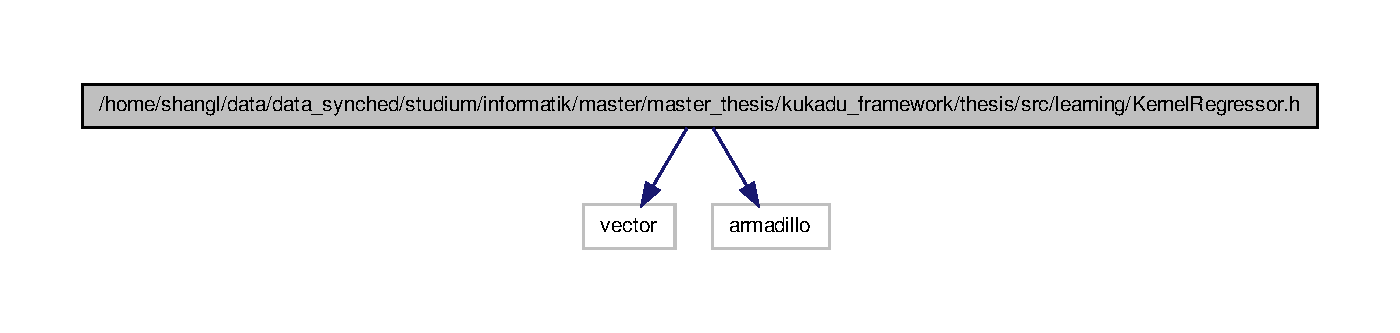
\includegraphics[width=350pt]{KernelRegressor_8h__incl}
\end{center}
\end{figure}
\-This graph shows which files directly or indirectly include this file\-:\nopagebreak
\begin{figure}[H]
\begin{center}
\leavevmode
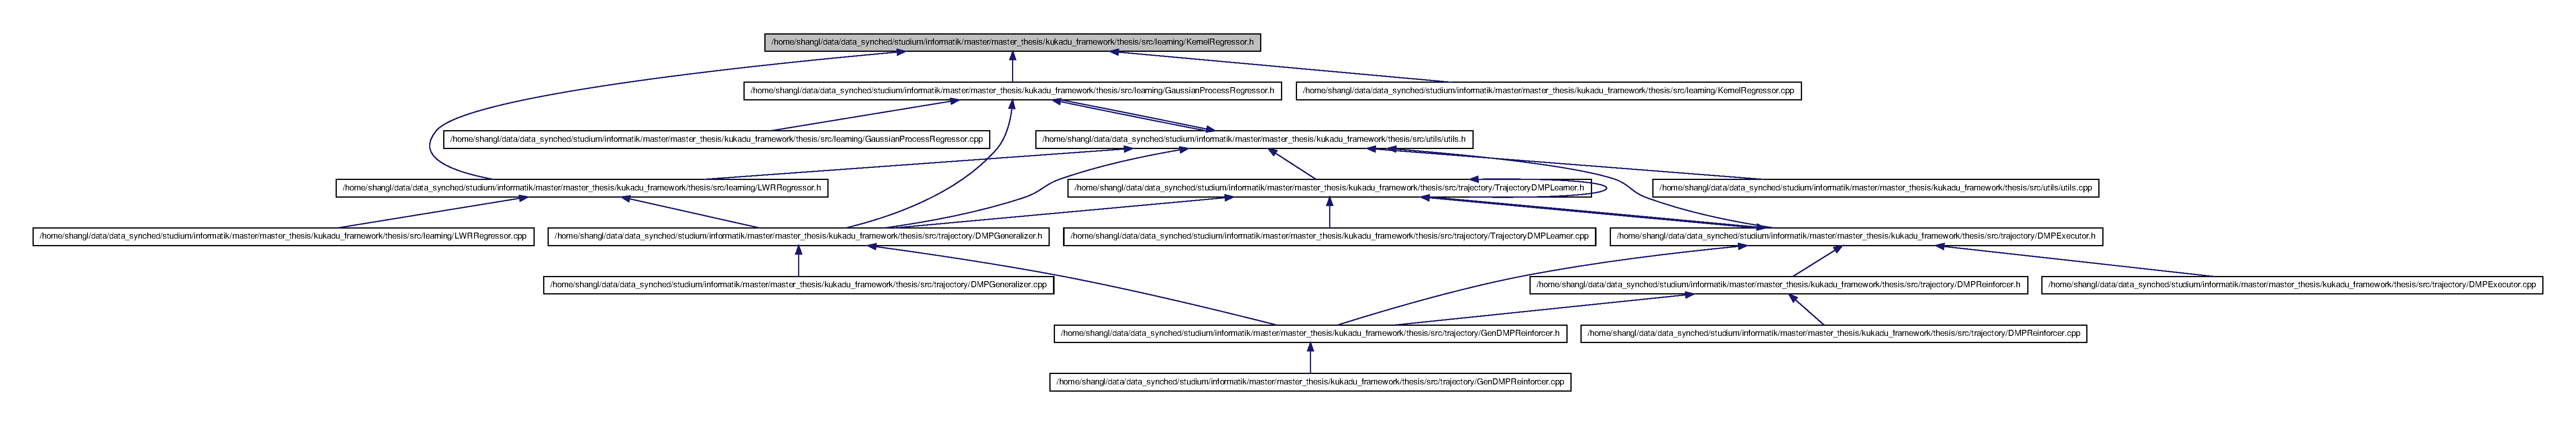
\includegraphics[width=350pt]{KernelRegressor_8h__dep__incl}
\end{center}
\end{figure}
\subsection*{\-Classes}
\begin{DoxyCompactItemize}
\item 
class \hyperlink{classKernelRegressor}{\-Kernel\-Regressor}
\begin{DoxyCompactList}\small\item\em \-Provides arbitrary interface for kernel methods. \end{DoxyCompactList}\end{DoxyCompactItemize}

\hypertarget{LWRRegressor_8cpp}{\section{/home/shangl/data/data\-\_\-synched/studium/informatik/master/master\-\_\-thesis/kukadu\-\_\-framework/thesis/src/learning/\-L\-W\-R\-Regressor.cpp \-File \-Reference}
\label{LWRRegressor_8cpp}\index{/home/shangl/data/data\-\_\-synched/studium/informatik/master/master\-\_\-thesis/kukadu\-\_\-framework/thesis/src/learning/\-L\-W\-R\-Regressor.\-cpp@{/home/shangl/data/data\-\_\-synched/studium/informatik/master/master\-\_\-thesis/kukadu\-\_\-framework/thesis/src/learning/\-L\-W\-R\-Regressor.\-cpp}}
}
{\ttfamily \#include \char`\"{}\-L\-W\-R\-Regressor.\-h\char`\"{}}\*
\-Include dependency graph for \-L\-W\-R\-Regressor.\-cpp\-:\nopagebreak
\begin{figure}[H]
\begin{center}
\leavevmode
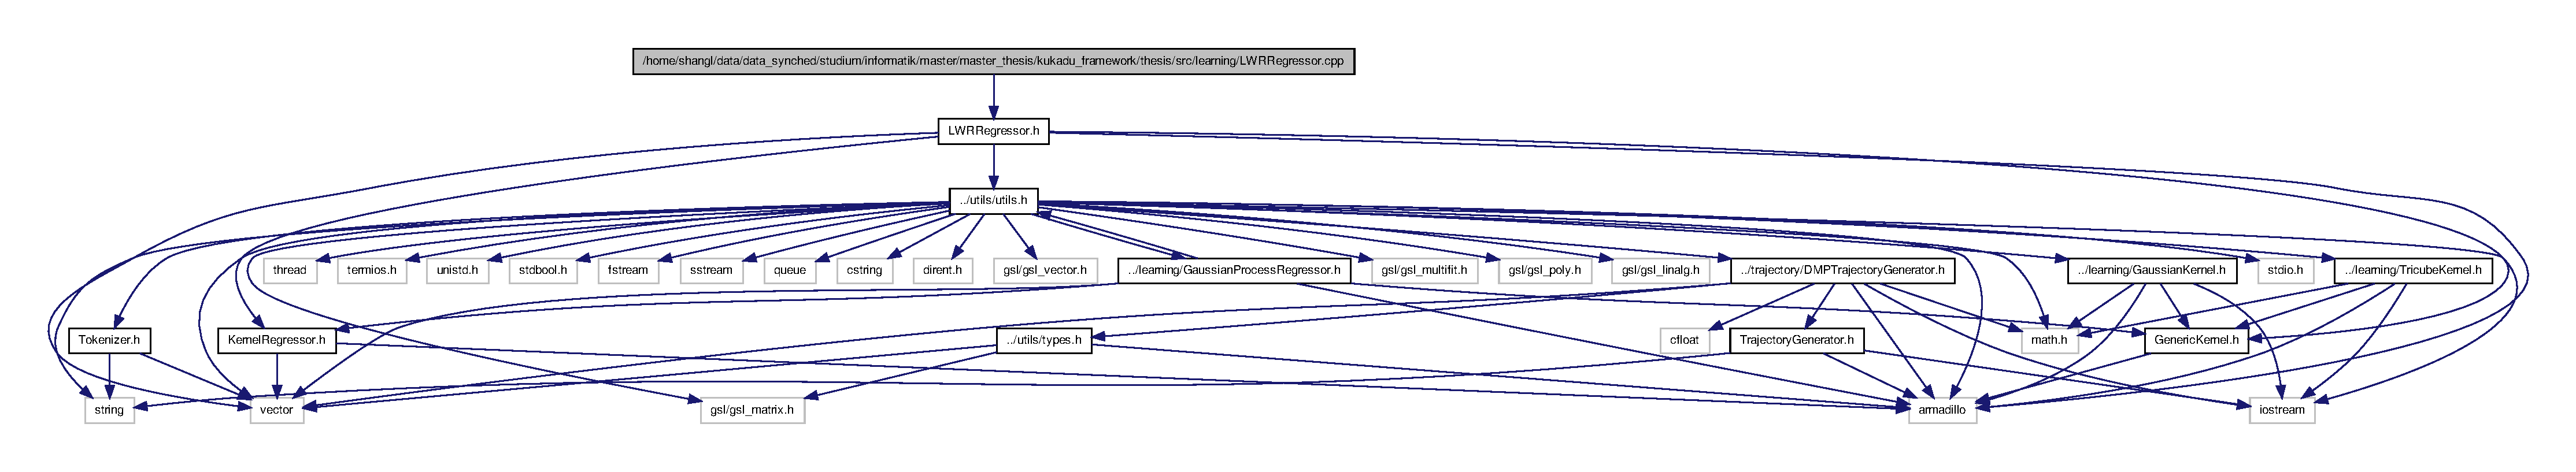
\includegraphics[width=350pt]{LWRRegressor_8cpp__incl}
\end{center}
\end{figure}

\hypertarget{LWRRegressor_8h}{\section{/home/shangl/data/data\-\_\-synched/studium/informatik/master/master\-\_\-thesis/kukadu\-\_\-framework/thesis/src/learning/\-L\-W\-R\-Regressor.h \-File \-Reference}
\label{LWRRegressor_8h}\index{/home/shangl/data/data\-\_\-synched/studium/informatik/master/master\-\_\-thesis/kukadu\-\_\-framework/thesis/src/learning/\-L\-W\-R\-Regressor.\-h@{/home/shangl/data/data\-\_\-synched/studium/informatik/master/master\-\_\-thesis/kukadu\-\_\-framework/thesis/src/learning/\-L\-W\-R\-Regressor.\-h}}
}
{\ttfamily \#include $<$armadillo$>$}\*
{\ttfamily \#include $<$vector$>$}\*
{\ttfamily \#include \char`\"{}\-Kernel\-Regressor.\-h\char`\"{}}\*
{\ttfamily \#include \char`\"{}\-Generic\-Kernel.\-h\char`\"{}}\*
{\ttfamily \#include \char`\"{}../utils/utils.\-h\char`\"{}}\*
\-Include dependency graph for \-L\-W\-R\-Regressor.\-h\-:\nopagebreak
\begin{figure}[H]
\begin{center}
\leavevmode
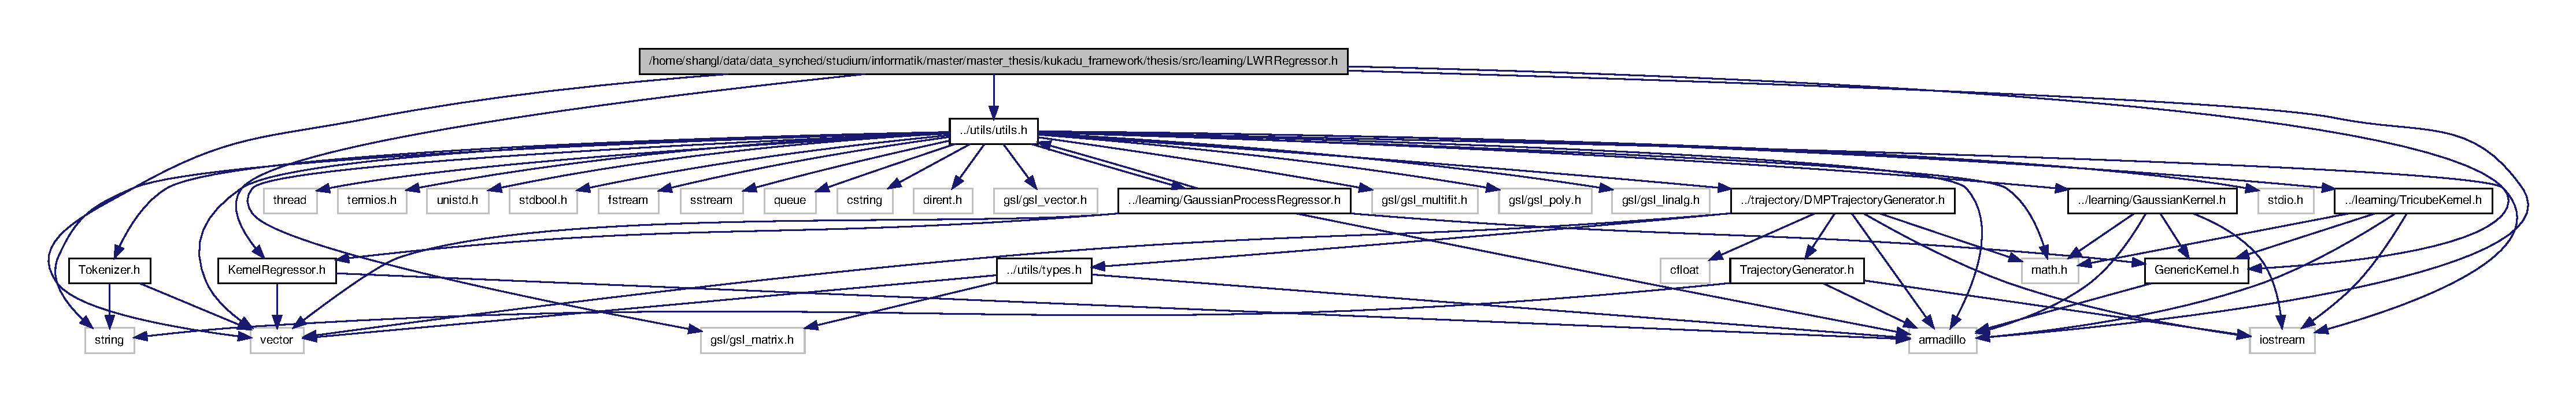
\includegraphics[width=350pt]{LWRRegressor_8h__incl}
\end{center}
\end{figure}
\-This graph shows which files directly or indirectly include this file\-:\nopagebreak
\begin{figure}[H]
\begin{center}
\leavevmode
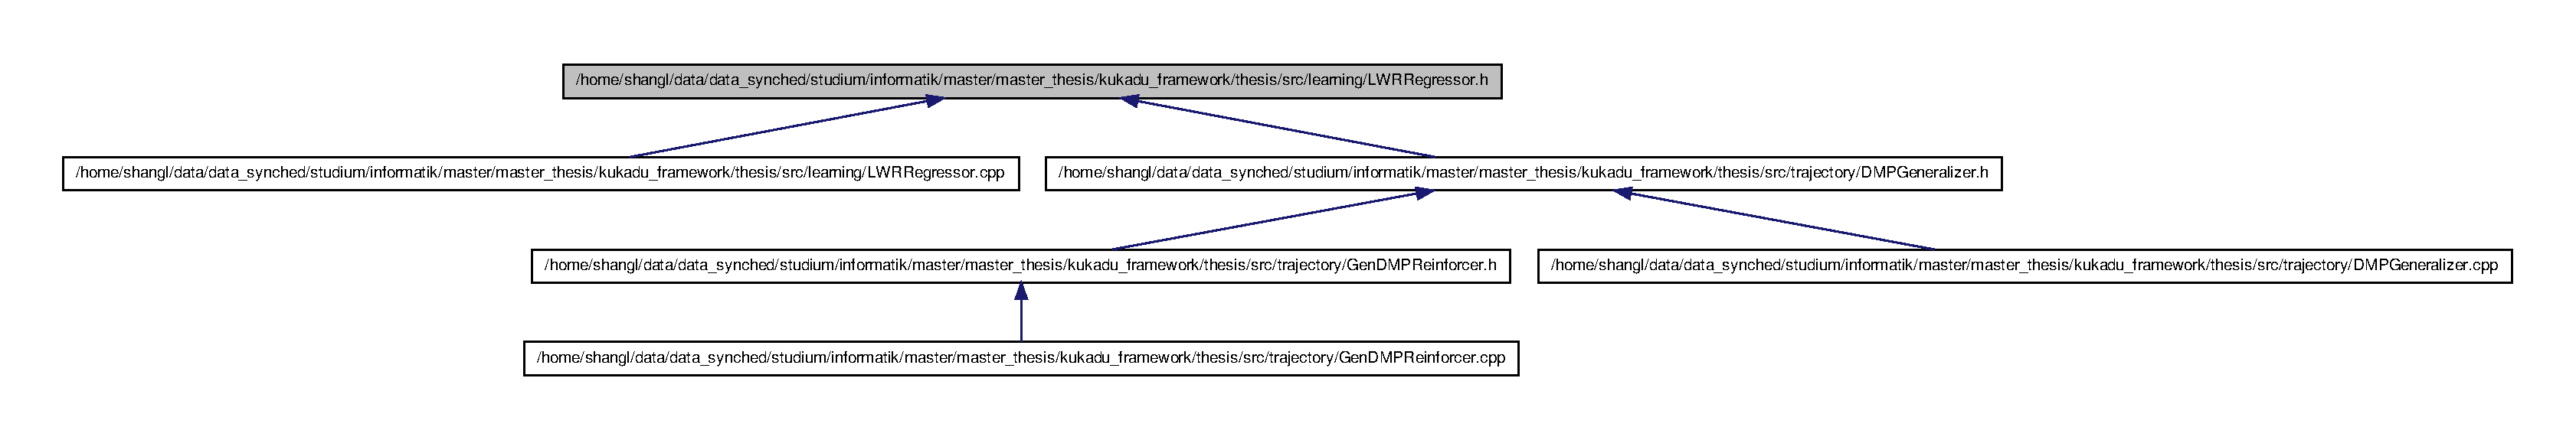
\includegraphics[width=350pt]{LWRRegressor_8h__dep__incl}
\end{center}
\end{figure}
\subsection*{\-Classes}
\begin{DoxyCompactItemize}
\item 
class \hyperlink{classLWRRegressor}{\-L\-W\-R\-Regressor}
\begin{DoxyCompactList}\small\item\em \-Implements the locally weighted regression method. \end{DoxyCompactList}\end{DoxyCompactItemize}

\hypertarget{QuadraticKernel_8cpp}{\section{/home/shangl/data/data\-\_\-synched/studium/informatik/master/master\-\_\-thesis/kukadu\-\_\-framework/thesis/src/learning/\-Quadratic\-Kernel.cpp \-File \-Reference}
\label{QuadraticKernel_8cpp}\index{/home/shangl/data/data\-\_\-synched/studium/informatik/master/master\-\_\-thesis/kukadu\-\_\-framework/thesis/src/learning/\-Quadratic\-Kernel.\-cpp@{/home/shangl/data/data\-\_\-synched/studium/informatik/master/master\-\_\-thesis/kukadu\-\_\-framework/thesis/src/learning/\-Quadratic\-Kernel.\-cpp}}
}
{\ttfamily \#include \char`\"{}\-Quadratic\-Kernel.\-h\char`\"{}}\*
\-Include dependency graph for \-Quadratic\-Kernel.\-cpp\-:\nopagebreak
\begin{figure}[H]
\begin{center}
\leavevmode
\includegraphics[width=350pt]{QuadraticKernel_8cpp__incl}
\end{center}
\end{figure}

\hypertarget{QuadraticKernel_8h}{\section{/home/shangl/data/data\-\_\-synched/studium/informatik/master/master\-\_\-thesis/kukadu\-\_\-framework/thesis/src/learning/\-Quadratic\-Kernel.h \-File \-Reference}
\label{QuadraticKernel_8h}\index{/home/shangl/data/data\-\_\-synched/studium/informatik/master/master\-\_\-thesis/kukadu\-\_\-framework/thesis/src/learning/\-Quadratic\-Kernel.\-h@{/home/shangl/data/data\-\_\-synched/studium/informatik/master/master\-\_\-thesis/kukadu\-\_\-framework/thesis/src/learning/\-Quadratic\-Kernel.\-h}}
}
{\ttfamily \#include \char`\"{}\-Generic\-Kernel.\-h\char`\"{}}\*
{\ttfamily \#include $<$armadillo$>$}\*
{\ttfamily \#include $<$math.\-h$>$}\*
{\ttfamily \#include $<$iostream$>$}\*
\-Include dependency graph for \-Quadratic\-Kernel.\-h\-:\nopagebreak
\begin{figure}[H]
\begin{center}
\leavevmode
\includegraphics[width=350pt]{QuadraticKernel_8h__incl}
\end{center}
\end{figure}
\-This graph shows which files directly or indirectly include this file\-:\nopagebreak
\begin{figure}[H]
\begin{center}
\leavevmode
\includegraphics[width=350pt]{QuadraticKernel_8h__dep__incl}
\end{center}
\end{figure}
\subsection*{\-Classes}
\begin{DoxyCompactItemize}
\item 
class \hyperlink{classQuadraticKernel}{\-Quadratic\-Kernel}
\begin{DoxyCompactList}\small\item\em \-Implements a quadratic kernel according to the \hyperlink{classGenericKernel}{\-Generic\-Kernel} specifiction. \end{DoxyCompactList}\end{DoxyCompactItemize}

\hypertarget{TricubeKernel_8cpp}{\section{/home/shangl/data/data\-\_\-synched/studium/informatik/master/master\-\_\-thesis/kukadu\-\_\-framework/thesis/src/learning/\-Tricube\-Kernel.cpp \-File \-Reference}
\label{TricubeKernel_8cpp}\index{/home/shangl/data/data\-\_\-synched/studium/informatik/master/master\-\_\-thesis/kukadu\-\_\-framework/thesis/src/learning/\-Tricube\-Kernel.\-cpp@{/home/shangl/data/data\-\_\-synched/studium/informatik/master/master\-\_\-thesis/kukadu\-\_\-framework/thesis/src/learning/\-Tricube\-Kernel.\-cpp}}
}
{\ttfamily \#include \char`\"{}\-Tricube\-Kernel.\-h\char`\"{}}\*
\-Include dependency graph for \-Tricube\-Kernel.\-cpp\-:\nopagebreak
\begin{figure}[H]
\begin{center}
\leavevmode
\includegraphics[width=350pt]{TricubeKernel_8cpp__incl}
\end{center}
\end{figure}

\hypertarget{TricubeKernel_8h}{\section{/home/shangl/data/data\-\_\-synched/studium/informatik/master/master\-\_\-thesis/kukadu\-\_\-framework/thesis/src/learning/\-Tricube\-Kernel.h \-File \-Reference}
\label{TricubeKernel_8h}\index{/home/shangl/data/data\-\_\-synched/studium/informatik/master/master\-\_\-thesis/kukadu\-\_\-framework/thesis/src/learning/\-Tricube\-Kernel.\-h@{/home/shangl/data/data\-\_\-synched/studium/informatik/master/master\-\_\-thesis/kukadu\-\_\-framework/thesis/src/learning/\-Tricube\-Kernel.\-h}}
}
{\ttfamily \#include \char`\"{}\-Generic\-Kernel.\-h\char`\"{}}\*
{\ttfamily \#include $<$armadillo$>$}\*
{\ttfamily \#include $<$math.\-h$>$}\*
{\ttfamily \#include $<$iostream$>$}\*
\-Include dependency graph for \-Tricube\-Kernel.\-h\-:\nopagebreak
\begin{figure}[H]
\begin{center}
\leavevmode
\includegraphics[width=350pt]{TricubeKernel_8h__incl}
\end{center}
\end{figure}
\-This graph shows which files directly or indirectly include this file\-:\nopagebreak
\begin{figure}[H]
\begin{center}
\leavevmode
\includegraphics[width=350pt]{TricubeKernel_8h__dep__incl}
\end{center}
\end{figure}
\subsection*{\-Classes}
\begin{DoxyCompactItemize}
\item 
class \hyperlink{classTricubeKernel}{\-Tricube\-Kernel}
\begin{DoxyCompactList}\small\item\em \-Implements a tricube kernel according to the \hyperlink{classGenericKernel}{\-Generic\-Kernel} specifiction. \end{DoxyCompactList}\end{DoxyCompactItemize}

\hypertarget{main_8cpp}{\section{/home/shangl/data/data\-\_\-synched/studium/informatik/master/master\-\_\-thesis/kukadu\-\_\-framework/thesis/src/main.cpp \-File \-Reference}
\label{main_8cpp}\index{/home/shangl/data/data\-\_\-synched/studium/informatik/master/master\-\_\-thesis/kukadu\-\_\-framework/thesis/src/main.\-cpp@{/home/shangl/data/data\-\_\-synched/studium/informatik/master/master\-\_\-thesis/kukadu\-\_\-framework/thesis/src/main.\-cpp}}
}
{\ttfamily \#include $<$stdio.\-h$>$}\*
{\ttfamily \#include $<$iostream$>$}\*
{\ttfamily \#include $<$fstream$>$}\*
{\ttfamily \#include $<$thread$>$}\*
{\ttfamily \#include $<$termios.\-h$>$}\*
{\ttfamily \#include $<$unistd.\-h$>$}\*
{\ttfamily \#include $<$queue$>$}\*
{\ttfamily \#include $<$gsl/gsl\-\_\-matrix.\-h$>$}\*
{\ttfamily \#include $<$gsl/gsl\-\_\-poly.\-h$>$}\*
{\ttfamily \#include $<$signal.\-h$>$}\*
{\ttfamily \#include $<$cfloat$>$}\*
{\ttfamily \#include $<$math.\-h$>$}\*
{\ttfamily \#include \char`\"{}../include/kukadu.\-h\char`\"{}}\*
\-Include dependency graph for main.\-cpp\-:\nopagebreak
\begin{figure}[H]
\begin{center}
\leavevmode
\includegraphics[width=350pt]{main_8cpp__incl}
\end{center}
\end{figure}
\subsection*{\-Functions}
\begin{DoxyCompactItemize}
\item 
char \hyperlink{main_8cpp_a9a8dfbe563aef804f9f437d2d64aeb72}{console\-Inputter} ()
\item 
void \hyperlink{main_8cpp_a9507713e376a62d245489612552aeb21}{got\-\_\-signal} (int)
\item 
int \hyperlink{main_8cpp_a7a29781a20c5dd4153c3c1cecf0ff328}{main} (int argc, char $\ast$$\ast$args)
\end{DoxyCompactItemize}
\subsection*{\-Variables}
\begin{DoxyCompactItemize}
\item 
char \hyperlink{main_8cpp_ab6911867f614168c67eb71fa7f8e4382}{console\-Input} = 0
\item 
vector$<$ \hyperlink{classDestroyableObject}{\-Destroyable\-Object} $\ast$ $>$ $\ast$ \hyperlink{main_8cpp_ae0546162205e4a4e616606ced5bffb3e}{destruct\-List} = \-N\-U\-L\-L
\end{DoxyCompactItemize}


\subsection{\-Function \-Documentation}
\hypertarget{main_8cpp_a9a8dfbe563aef804f9f437d2d64aeb72}{\index{main.\-cpp@{main.\-cpp}!console\-Inputter@{console\-Inputter}}
\index{console\-Inputter@{console\-Inputter}!main.cpp@{main.\-cpp}}
\subsubsection[{console\-Inputter}]{\setlength{\rightskip}{0pt plus 5cm}char {\bf console\-Inputter} (
\begin{DoxyParamCaption}
{}
\end{DoxyParamCaption}
)}}\label{main_8cpp_a9a8dfbe563aef804f9f437d2d64aeb72}
\hypertarget{main_8cpp_a9507713e376a62d245489612552aeb21}{\index{main.\-cpp@{main.\-cpp}!got\-\_\-signal@{got\-\_\-signal}}
\index{got\-\_\-signal@{got\-\_\-signal}!main.cpp@{main.\-cpp}}
\subsubsection[{got\-\_\-signal}]{\setlength{\rightskip}{0pt plus 5cm}void {\bf got\-\_\-signal} (
\begin{DoxyParamCaption}
\item[{int}]{in}
\end{DoxyParamCaption}
)}}\label{main_8cpp_a9507713e376a62d245489612552aeb21}
\hypertarget{main_8cpp_a7a29781a20c5dd4153c3c1cecf0ff328}{\index{main.\-cpp@{main.\-cpp}!main@{main}}
\index{main@{main}!main.cpp@{main.\-cpp}}
\subsubsection[{main}]{\setlength{\rightskip}{0pt plus 5cm}int {\bf main} (
\begin{DoxyParamCaption}
\item[{int}]{argc, }
\item[{char $\ast$$\ast$}]{args}
\end{DoxyParamCaption}
)}}\label{main_8cpp_a7a29781a20c5dd4153c3c1cecf0ff328}


\subsection{\-Variable \-Documentation}
\hypertarget{main_8cpp_ab6911867f614168c67eb71fa7f8e4382}{\index{main.\-cpp@{main.\-cpp}!console\-Input@{console\-Input}}
\index{console\-Input@{console\-Input}!main.cpp@{main.\-cpp}}
\subsubsection[{console\-Input}]{\setlength{\rightskip}{0pt plus 5cm}char {\bf console\-Input} = 0}}\label{main_8cpp_ab6911867f614168c67eb71fa7f8e4382}
\hypertarget{main_8cpp_ae0546162205e4a4e616606ced5bffb3e}{\index{main.\-cpp@{main.\-cpp}!destruct\-List@{destruct\-List}}
\index{destruct\-List@{destruct\-List}!main.cpp@{main.\-cpp}}
\subsubsection[{destruct\-List}]{\setlength{\rightskip}{0pt plus 5cm}vector$<${\bf \-Destroyable\-Object}$\ast$$>$$\ast$ {\bf destruct\-List} = \-N\-U\-L\-L}}\label{main_8cpp_ae0546162205e4a4e616606ced5bffb3e}

\hypertarget{mainDrill_8cpp}{\section{/home/shangl/data/data\-\_\-synched/studium/informatik/master/master\-\_\-thesis/kukadu\-\_\-framework/thesis/src/main\-Drill.cpp \-File \-Reference}
\label{mainDrill_8cpp}\index{/home/shangl/data/data\-\_\-synched/studium/informatik/master/master\-\_\-thesis/kukadu\-\_\-framework/thesis/src/main\-Drill.\-cpp@{/home/shangl/data/data\-\_\-synched/studium/informatik/master/master\-\_\-thesis/kukadu\-\_\-framework/thesis/src/main\-Drill.\-cpp}}
}
{\ttfamily \#include $<$stdio.\-h$>$}\*
{\ttfamily \#include $<$iostream$>$}\*
{\ttfamily \#include $<$fstream$>$}\*
{\ttfamily \#include $<$thread$>$}\*
{\ttfamily \#include $<$termios.\-h$>$}\*
{\ttfamily \#include $<$unistd.\-h$>$}\*
{\ttfamily \#include $<$queue$>$}\*
{\ttfamily \#include $<$gsl/gsl\-\_\-matrix.\-h$>$}\*
{\ttfamily \#include $<$gsl/gsl\-\_\-poly.\-h$>$}\*
{\ttfamily \#include $<$signal.\-h$>$}\*
{\ttfamily \#include \char`\"{}../include/kukadu.\-h\char`\"{}}\*
\-Include dependency graph for main\-Drill.\-cpp\-:\nopagebreak
\begin{figure}[H]
\begin{center}
\leavevmode
\includegraphics[width=350pt]{mainDrill_8cpp__incl}
\end{center}
\end{figure}
\subsection*{\-Functions}
\begin{DoxyCompactItemize}
\item 
char \hyperlink{mainDrill_8cpp_a9a8dfbe563aef804f9f437d2d64aeb72}{console\-Inputter} ()
\item 
void \hyperlink{mainDrill_8cpp_a9507713e376a62d245489612552aeb21}{got\-\_\-signal} (int)
\item 
int \hyperlink{mainDrill_8cpp_a7a29781a20c5dd4153c3c1cecf0ff328}{main} (int argc, char $\ast$$\ast$args)
\end{DoxyCompactItemize}
\subsection*{\-Variables}
\begin{DoxyCompactItemize}
\item 
char \hyperlink{mainDrill_8cpp_ab6911867f614168c67eb71fa7f8e4382}{console\-Input} = 0
\item 
vector$<$ \hyperlink{classDestroyableObject}{\-Destroyable\-Object} $\ast$ $>$ $\ast$ \hyperlink{mainDrill_8cpp_ae0546162205e4a4e616606ced5bffb3e}{destruct\-List} = \-N\-U\-L\-L
\end{DoxyCompactItemize}


\subsection{\-Function \-Documentation}
\hypertarget{mainDrill_8cpp_a9a8dfbe563aef804f9f437d2d64aeb72}{\index{main\-Drill.\-cpp@{main\-Drill.\-cpp}!console\-Inputter@{console\-Inputter}}
\index{console\-Inputter@{console\-Inputter}!mainDrill.cpp@{main\-Drill.\-cpp}}
\subsubsection[{console\-Inputter}]{\setlength{\rightskip}{0pt plus 5cm}char {\bf console\-Inputter} (
\begin{DoxyParamCaption}
{}
\end{DoxyParamCaption}
)}}\label{mainDrill_8cpp_a9a8dfbe563aef804f9f437d2d64aeb72}
\hypertarget{mainDrill_8cpp_a9507713e376a62d245489612552aeb21}{\index{main\-Drill.\-cpp@{main\-Drill.\-cpp}!got\-\_\-signal@{got\-\_\-signal}}
\index{got\-\_\-signal@{got\-\_\-signal}!mainDrill.cpp@{main\-Drill.\-cpp}}
\subsubsection[{got\-\_\-signal}]{\setlength{\rightskip}{0pt plus 5cm}void {\bf got\-\_\-signal} (
\begin{DoxyParamCaption}
\item[{int}]{in}
\end{DoxyParamCaption}
)}}\label{mainDrill_8cpp_a9507713e376a62d245489612552aeb21}
\hypertarget{mainDrill_8cpp_a7a29781a20c5dd4153c3c1cecf0ff328}{\index{main\-Drill.\-cpp@{main\-Drill.\-cpp}!main@{main}}
\index{main@{main}!mainDrill.cpp@{main\-Drill.\-cpp}}
\subsubsection[{main}]{\setlength{\rightskip}{0pt plus 5cm}int {\bf main} (
\begin{DoxyParamCaption}
\item[{int}]{argc, }
\item[{char $\ast$$\ast$}]{args}
\end{DoxyParamCaption}
)}}\label{mainDrill_8cpp_a7a29781a20c5dd4153c3c1cecf0ff328}


\subsection{\-Variable \-Documentation}
\hypertarget{mainDrill_8cpp_ab6911867f614168c67eb71fa7f8e4382}{\index{main\-Drill.\-cpp@{main\-Drill.\-cpp}!console\-Input@{console\-Input}}
\index{console\-Input@{console\-Input}!mainDrill.cpp@{main\-Drill.\-cpp}}
\subsubsection[{console\-Input}]{\setlength{\rightskip}{0pt plus 5cm}char {\bf console\-Input} = 0}}\label{mainDrill_8cpp_ab6911867f614168c67eb71fa7f8e4382}
\hypertarget{mainDrill_8cpp_ae0546162205e4a4e616606ced5bffb3e}{\index{main\-Drill.\-cpp@{main\-Drill.\-cpp}!destruct\-List@{destruct\-List}}
\index{destruct\-List@{destruct\-List}!mainDrill.cpp@{main\-Drill.\-cpp}}
\subsubsection[{destruct\-List}]{\setlength{\rightskip}{0pt plus 5cm}vector$<${\bf \-Destroyable\-Object}$\ast$$>$$\ast$ {\bf destruct\-List} = \-N\-U\-L\-L}}\label{mainDrill_8cpp_ae0546162205e4a4e616606ced5bffb3e}

\hypertarget{ControlQueue_8cpp}{\section{/home/shangl/data/data\-\_\-synched/studium/informatik/master/master\-\_\-thesis/kukadu\-\_\-framework/thesis/src/robot/\-Control\-Queue.cpp \-File \-Reference}
\label{ControlQueue_8cpp}\index{/home/shangl/data/data\-\_\-synched/studium/informatik/master/master\-\_\-thesis/kukadu\-\_\-framework/thesis/src/robot/\-Control\-Queue.\-cpp@{/home/shangl/data/data\-\_\-synched/studium/informatik/master/master\-\_\-thesis/kukadu\-\_\-framework/thesis/src/robot/\-Control\-Queue.\-cpp}}
}
{\ttfamily \#include \char`\"{}\-Control\-Queue.\-h\char`\"{}}\*
\-Include dependency graph for \-Control\-Queue.\-cpp\-:\nopagebreak
\begin{figure}[H]
\begin{center}
\leavevmode
\includegraphics[width=350pt]{ControlQueue_8cpp__incl}
\end{center}
\end{figure}

\hypertarget{ControlQueue_8h}{\section{/home/shangl/data/data\-\_\-synched/studium/informatik/master/master\-\_\-thesis/kukadu\-\_\-framework/thesis/src/robot/\-Control\-Queue.h \-File \-Reference}
\label{ControlQueue_8h}\index{/home/shangl/data/data\-\_\-synched/studium/informatik/master/master\-\_\-thesis/kukadu\-\_\-framework/thesis/src/robot/\-Control\-Queue.\-h@{/home/shangl/data/data\-\_\-synched/studium/informatik/master/master\-\_\-thesis/kukadu\-\_\-framework/thesis/src/robot/\-Control\-Queue.\-h}}
}
{\ttfamily \#include $<$thread$>$}\*
{\ttfamily \#include \char`\"{}../utils/\-Destroyable\-Object.\-h\char`\"{}}\*
{\ttfamily \#include \char`\"{}../utils/types.\-h\char`\"{}}\*
\-Include dependency graph for \-Control\-Queue.\-h\-:\nopagebreak
\begin{figure}[H]
\begin{center}
\leavevmode
\includegraphics[width=350pt]{ControlQueue_8h__incl}
\end{center}
\end{figure}
\-This graph shows which files directly or indirectly include this file\-:\nopagebreak
\begin{figure}[H]
\begin{center}
\leavevmode
\includegraphics[width=350pt]{ControlQueue_8h__dep__incl}
\end{center}
\end{figure}
\subsection*{\-Classes}
\begin{DoxyCompactItemize}
\item 
class \hyperlink{classControlQueue}{\-Control\-Queue}
\begin{DoxyCompactList}\small\item\em \-Provides an interface for robot controllers. \end{DoxyCompactList}\end{DoxyCompactItemize}
\subsection*{\-Defines}
\begin{DoxyCompactItemize}
\item 
\#define \hyperlink{ControlQueue_8h_a35e9b4ad804247e3b2b080d934bdb5f7}{\-C\-O\-M\-M\-A\-N\-D\-\_\-\-N\-O\-T\-\_\-\-S\-E\-T}~-\/100
\end{DoxyCompactItemize}


\subsection{\-Define \-Documentation}
\hypertarget{ControlQueue_8h_a35e9b4ad804247e3b2b080d934bdb5f7}{\index{\-Control\-Queue.\-h@{\-Control\-Queue.\-h}!\-C\-O\-M\-M\-A\-N\-D\-\_\-\-N\-O\-T\-\_\-\-S\-E\-T@{\-C\-O\-M\-M\-A\-N\-D\-\_\-\-N\-O\-T\-\_\-\-S\-E\-T}}
\index{\-C\-O\-M\-M\-A\-N\-D\-\_\-\-N\-O\-T\-\_\-\-S\-E\-T@{\-C\-O\-M\-M\-A\-N\-D\-\_\-\-N\-O\-T\-\_\-\-S\-E\-T}!ControlQueue.h@{\-Control\-Queue.\-h}}
\subsubsection[{\-C\-O\-M\-M\-A\-N\-D\-\_\-\-N\-O\-T\-\_\-\-S\-E\-T}]{\setlength{\rightskip}{0pt plus 5cm}\#define {\bf \-C\-O\-M\-M\-A\-N\-D\-\_\-\-N\-O\-T\-\_\-\-S\-E\-T}~-\/100}}\label{ControlQueue_8h_a35e9b4ad804247e3b2b080d934bdb5f7}

\hypertarget{KukaControlQueue_8cpp}{\section{/home/shangl/data/data\-\_\-synched/studium/informatik/master/master\-\_\-thesis/kukadu\-\_\-framework/thesis/src/robot/\-Kuka\-Control\-Queue.cpp \-File \-Reference}
\label{KukaControlQueue_8cpp}\index{/home/shangl/data/data\-\_\-synched/studium/informatik/master/master\-\_\-thesis/kukadu\-\_\-framework/thesis/src/robot/\-Kuka\-Control\-Queue.\-cpp@{/home/shangl/data/data\-\_\-synched/studium/informatik/master/master\-\_\-thesis/kukadu\-\_\-framework/thesis/src/robot/\-Kuka\-Control\-Queue.\-cpp}}
}
{\ttfamily \#include \char`\"{}\-Kuka\-Control\-Queue.\-h\char`\"{}}\*
{\ttfamily \#include $<$unistd.\-h$>$}\*
{\ttfamily \#include $<$queue$>$}\*
{\ttfamily \#include $<$iostream$>$}\*
{\ttfamily \#include $<$cstdlib$>$}\*
{\ttfamily \#include $<$math.\-h$>$}\*
{\ttfamily \#include $<$stdio.\-h$>$}\*
\-Include dependency graph for \-Kuka\-Control\-Queue.\-cpp\-:\nopagebreak
\begin{figure}[H]
\begin{center}
\leavevmode
\includegraphics[width=350pt]{KukaControlQueue_8cpp__incl}
\end{center}
\end{figure}
\subsection*{\-Defines}
\begin{DoxyCompactItemize}
\item 
\#define \hyperlink{KukaControlQueue_8cpp_a5afc95a50fb328fd45424ef54c2f68fd}{\-C\-O\-N\-T\-R\-O\-L\-Q\-U\-E\-U\-E\-\_\-\-D\-E\-B\-U\-G}~0
\end{DoxyCompactItemize}


\subsection{\-Define \-Documentation}
\hypertarget{KukaControlQueue_8cpp_a5afc95a50fb328fd45424ef54c2f68fd}{\index{\-Kuka\-Control\-Queue.\-cpp@{\-Kuka\-Control\-Queue.\-cpp}!\-C\-O\-N\-T\-R\-O\-L\-Q\-U\-E\-U\-E\-\_\-\-D\-E\-B\-U\-G@{\-C\-O\-N\-T\-R\-O\-L\-Q\-U\-E\-U\-E\-\_\-\-D\-E\-B\-U\-G}}
\index{\-C\-O\-N\-T\-R\-O\-L\-Q\-U\-E\-U\-E\-\_\-\-D\-E\-B\-U\-G@{\-C\-O\-N\-T\-R\-O\-L\-Q\-U\-E\-U\-E\-\_\-\-D\-E\-B\-U\-G}!KukaControlQueue.cpp@{\-Kuka\-Control\-Queue.\-cpp}}
\subsubsection[{\-C\-O\-N\-T\-R\-O\-L\-Q\-U\-E\-U\-E\-\_\-\-D\-E\-B\-U\-G}]{\setlength{\rightskip}{0pt plus 5cm}\#define {\bf \-C\-O\-N\-T\-R\-O\-L\-Q\-U\-E\-U\-E\-\_\-\-D\-E\-B\-U\-G}~0}}\label{KukaControlQueue_8cpp_a5afc95a50fb328fd45424ef54c2f68fd}

\hypertarget{KukaControlQueue_8h}{\section{/home/shangl/data/data\-\_\-synched/studium/informatik/master/master\-\_\-thesis/kukadu\-\_\-framework/thesis/src/robot/\-Kuka\-Control\-Queue.h \-File \-Reference}
\label{KukaControlQueue_8h}\index{/home/shangl/data/data\-\_\-synched/studium/informatik/master/master\-\_\-thesis/kukadu\-\_\-framework/thesis/src/robot/\-Kuka\-Control\-Queue.\-h@{/home/shangl/data/data\-\_\-synched/studium/informatik/master/master\-\_\-thesis/kukadu\-\_\-framework/thesis/src/robot/\-Kuka\-Control\-Queue.\-h}}
}
{\ttfamily \#include $<$unistd.\-h$>$}\*
{\ttfamily \#include $<$queue$>$}\*
{\ttfamily \#include $<$iostream$>$}\*
{\ttfamily \#include $<$cstdlib$>$}\*
{\ttfamily \#include $<$math.\-h$>$}\*
{\ttfamily \#include $<$thread$>$}\*
{\ttfamily \#include $<$mutex$>$}\*
{\ttfamily \#include $<$time.\-h$>$}\*
{\ttfamily \#include \char`\"{}\-Control\-Queue.\-h\char`\"{}}\*
{\ttfamily \#include \char`\"{}../utils/\-Destroyable\-Object.\-h\char`\"{}}\*
{\ttfamily \#include \char`\"{}../utils/types.\-h\char`\"{}}\*
{\ttfamily \#include \char`\"{}robot\-Driver/src/fri\-Main.\-h\char`\"{}}\*
{\ttfamily \#include \char`\"{}robot\-Driver/src/fri\-Misc.\-h\char`\"{}}\*
{\ttfamily \#include \char`\"{}robot\-Driver/src/kuka/fri\-Remote.\-h\char`\"{}}\*
\-Include dependency graph for \-Kuka\-Control\-Queue.\-h\-:\nopagebreak
\begin{figure}[H]
\begin{center}
\leavevmode
\includegraphics[width=350pt]{KukaControlQueue_8h__incl}
\end{center}
\end{figure}
\-This graph shows which files directly or indirectly include this file\-:\nopagebreak
\begin{figure}[H]
\begin{center}
\leavevmode
\includegraphics[width=350pt]{KukaControlQueue_8h__dep__incl}
\end{center}
\end{figure}
\subsection*{\-Classes}
\begin{DoxyCompactItemize}
\item 
class \hyperlink{classKukaControlQueue}{\-Kuka\-Control\-Queue}
\begin{DoxyCompactList}\small\item\em \-The \hyperlink{classKukaControlQueue}{\-Kuka\-Control\-Queue} provides control capabilities for the \-Kuka \-L\-W\-R 4+ robotic arm. \end{DoxyCompactList}\end{DoxyCompactItemize}
\subsection*{\-Defines}
\begin{DoxyCompactItemize}
\item 
\#define \hyperlink{KukaControlQueue_8h_a35e9b4ad804247e3b2b080d934bdb5f7}{\-C\-O\-M\-M\-A\-N\-D\-\_\-\-N\-O\-T\-\_\-\-S\-E\-T}~-\/100
\end{DoxyCompactItemize}


\subsection{\-Define \-Documentation}
\hypertarget{KukaControlQueue_8h_a35e9b4ad804247e3b2b080d934bdb5f7}{\index{\-Kuka\-Control\-Queue.\-h@{\-Kuka\-Control\-Queue.\-h}!\-C\-O\-M\-M\-A\-N\-D\-\_\-\-N\-O\-T\-\_\-\-S\-E\-T@{\-C\-O\-M\-M\-A\-N\-D\-\_\-\-N\-O\-T\-\_\-\-S\-E\-T}}
\index{\-C\-O\-M\-M\-A\-N\-D\-\_\-\-N\-O\-T\-\_\-\-S\-E\-T@{\-C\-O\-M\-M\-A\-N\-D\-\_\-\-N\-O\-T\-\_\-\-S\-E\-T}!KukaControlQueue.h@{\-Kuka\-Control\-Queue.\-h}}
\subsubsection[{\-C\-O\-M\-M\-A\-N\-D\-\_\-\-N\-O\-T\-\_\-\-S\-E\-T}]{\setlength{\rightskip}{0pt plus 5cm}\#define {\bf \-C\-O\-M\-M\-A\-N\-D\-\_\-\-N\-O\-T\-\_\-\-S\-E\-T}~-\/100}}\label{KukaControlQueue_8h_a35e9b4ad804247e3b2b080d934bdb5f7}

\hypertarget{GenericHand_8cpp}{\section{/home/shangl/data/data\-\_\-synched/studium/informatik/master/master\-\_\-thesis/kukadu\-\_\-framework/thesis/src/robot/mounted/\-Generic\-Hand.cpp \-File \-Reference}
\label{GenericHand_8cpp}\index{/home/shangl/data/data\-\_\-synched/studium/informatik/master/master\-\_\-thesis/kukadu\-\_\-framework/thesis/src/robot/mounted/\-Generic\-Hand.\-cpp@{/home/shangl/data/data\-\_\-synched/studium/informatik/master/master\-\_\-thesis/kukadu\-\_\-framework/thesis/src/robot/mounted/\-Generic\-Hand.\-cpp}}
}
{\ttfamily \#include \char`\"{}\-Generic\-Hand.\-h\char`\"{}}\*
\-Include dependency graph for \-Generic\-Hand.\-cpp\-:\nopagebreak
\begin{figure}[H]
\begin{center}
\leavevmode
\includegraphics[width=350pt]{GenericHand_8cpp__incl}
\end{center}
\end{figure}

\hypertarget{GenericHand_8h}{\section{/home/shangl/data/data\-\_\-synched/studium/informatik/master/master\-\_\-thesis/kukadu\-\_\-framework/thesis/src/robot/mounted/\-Generic\-Hand.h \-File \-Reference}
\label{GenericHand_8h}\index{/home/shangl/data/data\-\_\-synched/studium/informatik/master/master\-\_\-thesis/kukadu\-\_\-framework/thesis/src/robot/mounted/\-Generic\-Hand.\-h@{/home/shangl/data/data\-\_\-synched/studium/informatik/master/master\-\_\-thesis/kukadu\-\_\-framework/thesis/src/robot/mounted/\-Generic\-Hand.\-h}}
}
{\ttfamily \#include \char`\"{}../../utils/\-Destroyable\-Object.\-h\char`\"{}}\*
\-Include dependency graph for \-Generic\-Hand.\-h\-:\nopagebreak
\begin{figure}[H]
\begin{center}
\leavevmode
\includegraphics[width=350pt]{GenericHand_8h__incl}
\end{center}
\end{figure}
\-This graph shows which files directly or indirectly include this file\-:\nopagebreak
\begin{figure}[H]
\begin{center}
\leavevmode
\includegraphics[width=350pt]{GenericHand_8h__dep__incl}
\end{center}
\end{figure}
\subsection*{\-Classes}
\begin{DoxyCompactItemize}
\item 
class \hyperlink{classGenericHand}{\-Generic\-Hand}
\begin{DoxyCompactList}\small\item\em \-The \hyperlink{classGenericHand}{\-Generic\-Hand} provides a very elementary interface to control robot hands mounted on a robot arm \-This class provides very an interface for the very basic functionalities such as \char`\"{}connect to hand\char`\"{} or \char`\"{}close hand\char`\"{}. \end{DoxyCompactList}\end{DoxyCompactItemize}

\hypertarget{SchunkHand_8cpp}{\section{/home/shangl/data/data\-\_\-synched/studium/informatik/master/master\-\_\-thesis/kukadu\-\_\-framework/thesis/src/robot/mounted/\-Schunk\-Hand.cpp \-File \-Reference}
\label{SchunkHand_8cpp}\index{/home/shangl/data/data\-\_\-synched/studium/informatik/master/master\-\_\-thesis/kukadu\-\_\-framework/thesis/src/robot/mounted/\-Schunk\-Hand.\-cpp@{/home/shangl/data/data\-\_\-synched/studium/informatik/master/master\-\_\-thesis/kukadu\-\_\-framework/thesis/src/robot/mounted/\-Schunk\-Hand.\-cpp}}
}
{\ttfamily \#include \char`\"{}\-Schunk\-Hand.\-h\char`\"{}}\*
\-Include dependency graph for \-Schunk\-Hand.\-cpp\-:\nopagebreak
\begin{figure}[H]
\begin{center}
\leavevmode
\includegraphics[width=350pt]{SchunkHand_8cpp__incl}
\end{center}
\end{figure}

\hypertarget{SchunkHand_8h}{\section{/home/shangl/data/data\-\_\-synched/studium/informatik/master/master\-\_\-thesis/kukadu\-\_\-framework/thesis/src/robot/mounted/\-Schunk\-Hand.h \-File \-Reference}
\label{SchunkHand_8h}\index{/home/shangl/data/data\-\_\-synched/studium/informatik/master/master\-\_\-thesis/kukadu\-\_\-framework/thesis/src/robot/mounted/\-Schunk\-Hand.\-h@{/home/shangl/data/data\-\_\-synched/studium/informatik/master/master\-\_\-thesis/kukadu\-\_\-framework/thesis/src/robot/mounted/\-Schunk\-Hand.\-h}}
}
{\ttfamily \#include $<$iostream$>$}\*
{\ttfamily \#include \char`\"{}\-Generic\-Hand.\-h\char`\"{}}\*
{\ttfamily \#include \char`\"{}sdh/sdh.\-h\char`\"{}}\*
{\ttfamily \#include \char`\"{}sdh/util.\-h\char`\"{}}\*
{\ttfamily \#include \char`\"{}sdh/sdhlibrary\-\_\-settings.\-h\char`\"{}}\*
{\ttfamily \#include \char`\"{}sdh/basisdef.\-h\char`\"{}}\*
{\ttfamily \#include \char`\"{}sdhoptions.\-h\char`\"{}}\*
\-Include dependency graph for \-Schunk\-Hand.\-h\-:\nopagebreak
\begin{figure}[H]
\begin{center}
\leavevmode
\includegraphics[width=350pt]{SchunkHand_8h__incl}
\end{center}
\end{figure}
\-This graph shows which files directly or indirectly include this file\-:\nopagebreak
\begin{figure}[H]
\begin{center}
\leavevmode
\includegraphics[width=350pt]{SchunkHand_8h__dep__incl}
\end{center}
\end{figure}
\subsection*{\-Classes}
\begin{DoxyCompactItemize}
\item 
class \hyperlink{classSchunkHand}{\-Schunk\-Hand}
\begin{DoxyCompactList}\small\item\em \-Provides control capabilities for the \-Schunk \-S\-D\-H robotic hand \-Implements the \hyperlink{classGenericHand}{\-Generic\-Hand} interface for the \-Schunk \-S\-D\-H robotic hand. \-Note that using this class the programm has to be executed with root rights. \end{DoxyCompactList}\end{DoxyCompactItemize}

\hypertarget{sdhoptions_8cpp}{\section{/home/shangl/data/data\-\_\-synched/studium/informatik/master/master\-\_\-thesis/kukadu\-\_\-framework/thesis/src/robot/mounted/sdhoptions.cpp \-File \-Reference}
\label{sdhoptions_8cpp}\index{/home/shangl/data/data\-\_\-synched/studium/informatik/master/master\-\_\-thesis/kukadu\-\_\-framework/thesis/src/robot/mounted/sdhoptions.\-cpp@{/home/shangl/data/data\-\_\-synched/studium/informatik/master/master\-\_\-thesis/kukadu\-\_\-framework/thesis/src/robot/mounted/sdhoptions.\-cpp}}
}


\-Implementation of a class to parse common \-S\-D\-H related command line options.  


{\ttfamily \#include $<$getopt.\-h$>$}\*
{\ttfamily \#include $<$assert.\-h$>$}\*
{\ttfamily \#include $<$iostream$>$}\*
{\ttfamily \#include $<$fstream$>$}\*
{\ttfamily \#include \char`\"{}sdh/sdh.\-h\char`\"{}}\*
{\ttfamily \#include \char`\"{}sdh/sdhlibrary\-\_\-settings.\-h\char`\"{}}\*
{\ttfamily \#include \char`\"{}sdh/release.\-h\char`\"{}}\*
{\ttfamily \#include \char`\"{}sdh/dsa.\-h\char`\"{}}\*
{\ttfamily \#include \char`\"{}sdhoptions.\-h\char`\"{}}\*
\-Include dependency graph for sdhoptions.\-cpp\-:\nopagebreak
\begin{figure}[H]
\begin{center}
\leavevmode
\includegraphics[width=350pt]{sdhoptions_8cpp__incl}
\end{center}
\end{figure}
\subsection*{\-Defines}
\begin{DoxyCompactItemize}
\item 
\#define \hyperlink{sdhoptions_8cpp_a5b45b6c1829ae4e062bceb78cbba002e}{\-X\-S\-T\-R\-I\-N\-G\-I\-F\-Y}(\-\_\-x)~\hyperlink{sdhoptions_8cpp_a0f4bf94ce01a331da306b94310faf208}{\-S\-T\-R\-I\-N\-G\-I\-F\-Y}(\-\_\-x)
\item 
\#define \hyperlink{sdhoptions_8cpp_a0f4bf94ce01a331da306b94310faf208}{\-S\-T\-R\-I\-N\-G\-I\-F\-Y}(\-\_\-s)~\#\-\_\-s
\begin{DoxyCompactList}\small\item\em helper macro for \-X\-S\-T\-R\-I\-N\-G\-I\-F\-Y, see there \end{DoxyCompactList}\end{DoxyCompactItemize}


\subsection{\-Detailed \-Description}
\begin{DoxyAuthor}{\-Author}
\-Dirk \-Osswald 
\end{DoxyAuthor}
\begin{DoxyDate}{\-Date}
2008-\/05-\/05
\end{DoxyDate}
\hypertarget{sdhoptions_8cpp_sdhlibrary_cpp_demo_sdhoptions_cpp_copyright}{}\subsection{\-Copyright}\label{sdhoptions_8cpp_sdhlibrary_cpp_demo_sdhoptions_cpp_copyright}
\-Copyright (c) 2008 \-S\-C\-H\-U\-N\-K \-Gmb\-H \& \-Co. \-K\-G



 

\subsection{\-Define \-Documentation}
\hypertarget{sdhoptions_8cpp_a0f4bf94ce01a331da306b94310faf208}{\index{sdhoptions.\-cpp@{sdhoptions.\-cpp}!\-S\-T\-R\-I\-N\-G\-I\-F\-Y@{\-S\-T\-R\-I\-N\-G\-I\-F\-Y}}
\index{\-S\-T\-R\-I\-N\-G\-I\-F\-Y@{\-S\-T\-R\-I\-N\-G\-I\-F\-Y}!sdhoptions.cpp@{sdhoptions.\-cpp}}
\subsubsection[{\-S\-T\-R\-I\-N\-G\-I\-F\-Y}]{\setlength{\rightskip}{0pt plus 5cm}\#define {\bf \-S\-T\-R\-I\-N\-G\-I\-F\-Y}(
\begin{DoxyParamCaption}
\item[{}]{\-\_\-s}
\end{DoxyParamCaption}
)~\#\-\_\-s}}\label{sdhoptions_8cpp_a0f4bf94ce01a331da306b94310faf208}
\hypertarget{sdhoptions_8cpp_a5b45b6c1829ae4e062bceb78cbba002e}{\index{sdhoptions.\-cpp@{sdhoptions.\-cpp}!\-X\-S\-T\-R\-I\-N\-G\-I\-F\-Y@{\-X\-S\-T\-R\-I\-N\-G\-I\-F\-Y}}
\index{\-X\-S\-T\-R\-I\-N\-G\-I\-F\-Y@{\-X\-S\-T\-R\-I\-N\-G\-I\-F\-Y}!sdhoptions.cpp@{sdhoptions.\-cpp}}
\subsubsection[{\-X\-S\-T\-R\-I\-N\-G\-I\-F\-Y}]{\setlength{\rightskip}{0pt plus 5cm}\#define {\bf \-X\-S\-T\-R\-I\-N\-G\-I\-F\-Y}(
\begin{DoxyParamCaption}
\item[{}]{\-\_\-x}
\end{DoxyParamCaption}
)~{\bf \-S\-T\-R\-I\-N\-G\-I\-F\-Y}(\-\_\-x)}}\label{sdhoptions_8cpp_a5b45b6c1829ae4e062bceb78cbba002e}
macro for stringification of {\itshape \-\_\-x\/} 

allows to stringify the {\bfseries value} of a macro\-: 
\begin{DoxyCode}
   #define foo 4

   STRINGIFY( foo ) // yields "foo"
   XSTRINGIFY( foo ) // yields "4"
\end{DoxyCode}
 
\hypertarget{sdhoptions_8h}{\section{/home/shangl/data/data\-\_\-synched/studium/informatik/master/master\-\_\-thesis/kukadu\-\_\-framework/thesis/src/robot/mounted/sdhoptions.h \-File \-Reference}
\label{sdhoptions_8h}\index{/home/shangl/data/data\-\_\-synched/studium/informatik/master/master\-\_\-thesis/kukadu\-\_\-framework/thesis/src/robot/mounted/sdhoptions.\-h@{/home/shangl/data/data\-\_\-synched/studium/informatik/master/master\-\_\-thesis/kukadu\-\_\-framework/thesis/src/robot/mounted/sdhoptions.\-h}}
}


\-Implementation of a class to parse common \-S\-D\-H related command line options.  


{\ttfamily \#include $<$getopt.\-h$>$}\*
{\ttfamily \#include $<$assert.\-h$>$}\*
{\ttfamily \#include $<$iostream$>$}\*
{\ttfamily \#include $<$string$>$}\*
{\ttfamily \#include $<$sdh/sdh.\-h$>$}\*
\-Include dependency graph for sdhoptions.\-h\-:\nopagebreak
\begin{figure}[H]
\begin{center}
\leavevmode
\includegraphics[width=350pt]{sdhoptions_8h__incl}
\end{center}
\end{figure}
\-This graph shows which files directly or indirectly include this file\-:\nopagebreak
\begin{figure}[H]
\begin{center}
\leavevmode
\includegraphics[width=350pt]{sdhoptions_8h__dep__incl}
\end{center}
\end{figure}
\subsection*{\-Classes}
\begin{DoxyCompactItemize}
\item 
class \hyperlink{classcSDHOptions}{c\-S\-D\-H\-Options}
\begin{DoxyCompactList}\small\item\em class for command line option parsing holding option parsing results \end{DoxyCompactList}\end{DoxyCompactItemize}
\subsection*{\-Defines}
\begin{DoxyCompactItemize}
\item 
\#define \hyperlink{sdhoptions_8h_a90372ef85e86e456fa18741a81f9b81d}{\-S\-D\-H\-U\-S\-A\-G\-E\-\_\-\-D\-E\-F\-A\-U\-L\-T}~\char`\"{}general sdhcom\-\_\-serial sdhcom\-\_\-common sdhcom\-\_\-esdcan sdhcom\-\_\-peakcan sdhcom\-\_\-cancommon sdhcom\-\_\-tcp\char`\"{}
\item 
\#define \hyperlink{sdhoptions_8h_a4ef64847cfd080bd39184e7d05ef003e}{\-S\-D\-H\-\_\-\-D\-E\-F\-A\-U\-L\-T\-\_\-\-T\-C\-P\-\_\-\-A\-D\-R}~\char`\"{}192.\-168.\-1.\-1\char`\"{}
\item 
\#define \hyperlink{sdhoptions_8h_a4048b8090a1b2ec460add90f2703c7d9}{\-S\-D\-H\-\_\-\-D\-E\-F\-A\-U\-L\-T\-\_\-\-T\-C\-P\-\_\-\-P\-O\-R\-T}~23
\end{DoxyCompactItemize}


\subsection{\-Detailed \-Description}
\hypertarget{sdhoptions_8h_sdhlibrary_cpp_demo_sdhoptions_h_general}{}\subsection{\-General file information}\label{sdhoptions_8h_sdhlibrary_cpp_demo_sdhoptions_h_general}
\begin{DoxyAuthor}{\-Author}
\-Dirk \-Osswald 
\end{DoxyAuthor}
\begin{DoxyDate}{\-Date}
2008-\/05-\/05
\end{DoxyDate}
\hypertarget{sdhoptions_8h_sdhlibrary_cpp_demo_sdhoptions_h_copyright}{}\subsection{\-Copyright}\label{sdhoptions_8h_sdhlibrary_cpp_demo_sdhoptions_h_copyright}
\-Copyright (c) 2008 \-S\-C\-H\-U\-N\-K \-Gmb\-H \& \-Co. \-K\-G



 

\subsection{\-Define \-Documentation}
\hypertarget{sdhoptions_8h_a4ef64847cfd080bd39184e7d05ef003e}{\index{sdhoptions.\-h@{sdhoptions.\-h}!\-S\-D\-H\-\_\-\-D\-E\-F\-A\-U\-L\-T\-\_\-\-T\-C\-P\-\_\-\-A\-D\-R@{\-S\-D\-H\-\_\-\-D\-E\-F\-A\-U\-L\-T\-\_\-\-T\-C\-P\-\_\-\-A\-D\-R}}
\index{\-S\-D\-H\-\_\-\-D\-E\-F\-A\-U\-L\-T\-\_\-\-T\-C\-P\-\_\-\-A\-D\-R@{\-S\-D\-H\-\_\-\-D\-E\-F\-A\-U\-L\-T\-\_\-\-T\-C\-P\-\_\-\-A\-D\-R}!sdhoptions.h@{sdhoptions.\-h}}
\subsubsection[{\-S\-D\-H\-\_\-\-D\-E\-F\-A\-U\-L\-T\-\_\-\-T\-C\-P\-\_\-\-A\-D\-R}]{\setlength{\rightskip}{0pt plus 5cm}\#define {\bf \-S\-D\-H\-\_\-\-D\-E\-F\-A\-U\-L\-T\-\_\-\-T\-C\-P\-\_\-\-A\-D\-R}~\char`\"{}192.\-168.\-1.\-1\char`\"{}}}\label{sdhoptions_8h_a4ef64847cfd080bd39184e7d05ef003e}
\hypertarget{sdhoptions_8h_a4048b8090a1b2ec460add90f2703c7d9}{\index{sdhoptions.\-h@{sdhoptions.\-h}!\-S\-D\-H\-\_\-\-D\-E\-F\-A\-U\-L\-T\-\_\-\-T\-C\-P\-\_\-\-P\-O\-R\-T@{\-S\-D\-H\-\_\-\-D\-E\-F\-A\-U\-L\-T\-\_\-\-T\-C\-P\-\_\-\-P\-O\-R\-T}}
\index{\-S\-D\-H\-\_\-\-D\-E\-F\-A\-U\-L\-T\-\_\-\-T\-C\-P\-\_\-\-P\-O\-R\-T@{\-S\-D\-H\-\_\-\-D\-E\-F\-A\-U\-L\-T\-\_\-\-T\-C\-P\-\_\-\-P\-O\-R\-T}!sdhoptions.h@{sdhoptions.\-h}}
\subsubsection[{\-S\-D\-H\-\_\-\-D\-E\-F\-A\-U\-L\-T\-\_\-\-T\-C\-P\-\_\-\-P\-O\-R\-T}]{\setlength{\rightskip}{0pt plus 5cm}\#define {\bf \-S\-D\-H\-\_\-\-D\-E\-F\-A\-U\-L\-T\-\_\-\-T\-C\-P\-\_\-\-P\-O\-R\-T}~23}}\label{sdhoptions_8h_a4048b8090a1b2ec460add90f2703c7d9}
\hypertarget{sdhoptions_8h_a90372ef85e86e456fa18741a81f9b81d}{\index{sdhoptions.\-h@{sdhoptions.\-h}!\-S\-D\-H\-U\-S\-A\-G\-E\-\_\-\-D\-E\-F\-A\-U\-L\-T@{\-S\-D\-H\-U\-S\-A\-G\-E\-\_\-\-D\-E\-F\-A\-U\-L\-T}}
\index{\-S\-D\-H\-U\-S\-A\-G\-E\-\_\-\-D\-E\-F\-A\-U\-L\-T@{\-S\-D\-H\-U\-S\-A\-G\-E\-\_\-\-D\-E\-F\-A\-U\-L\-T}!sdhoptions.h@{sdhoptions.\-h}}
\subsubsection[{\-S\-D\-H\-U\-S\-A\-G\-E\-\_\-\-D\-E\-F\-A\-U\-L\-T}]{\setlength{\rightskip}{0pt plus 5cm}\#define {\bf \-S\-D\-H\-U\-S\-A\-G\-E\-\_\-\-D\-E\-F\-A\-U\-L\-T}~\char`\"{}general sdhcom\-\_\-serial sdhcom\-\_\-common sdhcom\-\_\-esdcan sdhcom\-\_\-peakcan sdhcom\-\_\-cancommon sdhcom\-\_\-tcp\char`\"{}}}\label{sdhoptions_8h_a90372ef85e86e456fa18741a81f9b81d}
string defining all the usage helptexts included by default

\begin{DoxyRefDesc}{\-Bug}
\item[\hyperlink{bug__bug000001}{\-Bug}]\-When compiled with \-V\-C\-C then the macros \-W\-I\-T\-H\-\_\-\-E\-S\-D\-\_\-\-C\-A\-N / \-W\-I\-T\-H\-\_\-\-P\-E\-A\-K\-\_\-\-C\-A\-N used above are not available since these are defined in the \-V\-C\-C project settings of the \-S\-D\-H\-Library \-V\-C\-C-\/\-Project. \-Therefore the value of \-S\-D\-H\-U\-S\-A\-G\-E\-\_\-\-D\-E\-F\-A\-U\-L\-T is incorrect and thus the \hyperlink{classcSDHOptions}{c\-S\-D\-H\-Options} will display an incomplete usage string when called with -\/h/-\/-\/help.\par
 \-Workaround\-: use the online help contained in the doxygen documentation\-: \href{./group__sdh__library__cpp__onlinehelp__group.html}{\tt \-Online help of demonstration programs} \end{DoxyRefDesc}

\hypertarget{testHand_8cpp}{\section{/home/shangl/data/data\-\_\-synched/studium/informatik/master/master\-\_\-thesis/kukadu\-\_\-framework/thesis/src/robot/mounted/test\-Hand.cpp \-File \-Reference}
\label{testHand_8cpp}\index{/home/shangl/data/data\-\_\-synched/studium/informatik/master/master\-\_\-thesis/kukadu\-\_\-framework/thesis/src/robot/mounted/test\-Hand.\-cpp@{/home/shangl/data/data\-\_\-synched/studium/informatik/master/master\-\_\-thesis/kukadu\-\_\-framework/thesis/src/robot/mounted/test\-Hand.\-cpp}}
}
{\ttfamily \#include $<$iostream$>$}\*
{\ttfamily \#include $<$vector$>$}\*
{\ttfamily \#include \char`\"{}sdh/sdh.\-h\char`\"{}}\*
{\ttfamily \#include \char`\"{}sdh/util.\-h\char`\"{}}\*
{\ttfamily \#include \char`\"{}sdh/sdhlibrary\-\_\-settings.\-h\char`\"{}}\*
{\ttfamily \#include \char`\"{}sdh/basisdef.\-h\char`\"{}}\*
{\ttfamily \#include \char`\"{}sdhoptions.\-h\char`\"{}}\*
\-Include dependency graph for test\-Hand.\-cpp\-:\nopagebreak
\begin{figure}[H]
\begin{center}
\leavevmode
\includegraphics[width=350pt]{testHand_8cpp__incl}
\end{center}
\end{figure}
\subsection*{\-Functions}
\begin{DoxyCompactItemize}
\item 
\-U\-S\-I\-N\-G\-\_\-\-N\-A\-M\-E\-S\-P\-A\-C\-E\-\_\-\-S\-D\-H int \hyperlink{testHand_8cpp_a54ce7579ed08b96d36a43c6f878a1a61}{main} (int argc, char $\ast$$\ast$argv)
\end{DoxyCompactItemize}


\subsection{\-Function \-Documentation}
\hypertarget{testHand_8cpp_a54ce7579ed08b96d36a43c6f878a1a61}{\index{test\-Hand.\-cpp@{test\-Hand.\-cpp}!main@{main}}
\index{main@{main}!testHand.cpp@{test\-Hand.\-cpp}}
\subsubsection[{main}]{\setlength{\rightskip}{0pt plus 5cm}\-U\-S\-I\-N\-G\-\_\-\-N\-A\-M\-E\-S\-P\-A\-C\-E\-\_\-\-S\-D\-H int {\bf main} (
\begin{DoxyParamCaption}
\item[{int}]{argc, }
\item[{char $\ast$$\ast$}]{argv}
\end{DoxyParamCaption}
)}}\label{testHand_8cpp_a54ce7579ed08b96d36a43c6f878a1a61}

\hypertarget{fri__example_8m}{\section{/home/shangl/data/data\-\_\-synched/studium/informatik/master/master\-\_\-thesis/kukadu\-\_\-framework/thesis/src/robot/robot\-Driver/matlab/fri\-\_\-example.m \-File \-Reference}
\label{fri__example_8m}\index{/home/shangl/data/data\-\_\-synched/studium/informatik/master/master\-\_\-thesis/kukadu\-\_\-framework/thesis/src/robot/robot\-Driver/matlab/fri\-\_\-example.\-m@{/home/shangl/data/data\-\_\-synched/studium/informatik/master/master\-\_\-thesis/kukadu\-\_\-framework/thesis/src/robot/robot\-Driver/matlab/fri\-\_\-example.\-m}}
}
\subsection*{\-Functions}
\begin{DoxyCompactItemize}
\item 
\hyperlink{fri__example_8m_ab02121d4dfeb622a4ea3db42c0cb6676}{pause} ()
\item 
\hyperlink{fri__example_8m_ace6453c265aedf6f6d285350c6f6a7ec}{pause} (0.\-5)
\item 
\-Get current \hyperlink{fri__example_8m_a6b7c93a885b43441f4e04026891e8c69}{position} \hyperlink{fri__example_8m_a3f1af79c2714428551003be46c6d708b}{position} (1)
\item 
\hyperlink{fri__example_8m_a55a5df3a7b663404df4842cd61f2be6e}{position} (2)
\item 
\hyperlink{fri__example_8m_a6b7c93a885b43441f4e04026891e8c69}{position} (3)
\end{DoxyCompactItemize}
\subsection*{\-Variables}
\begin{DoxyCompactItemize}
\item 
\hyperlink{fri__example_8m_ab2a433e8d210d6c486f07daa68d0c1e3}{listenning\-Port} = 49938
\item 
\hyperlink{fri__example_8m_a094bd681592faefb6f9be3d22d34cbcd}{joints} = fri\-\_\-get\-Joints(\hyperlink{fri__example_8m_ab2a433e8d210d6c486f07daa68d0c1e3}{listenning\-Port})
\item 
\hyperlink{fri__example_8m_a5a07df8b8eb38bfae207b096d812d129}{current\-Joints}
\item 
\hyperlink{fri__example_8m_a5c3f4f63b5943ddebdb542e2dd1f3a67}{safe\-Joints} = \mbox{[}0.\-0785 0.\-0349 0 1.\-2392 0 -\/0.\-7679 0.\-0175\mbox{]}
\item 
\hyperlink{fri__example_8m_ae24e0aa52547e9504f585c14dca7b165}{home\-Joints} = \mbox{[}0 0 0 0 0 0 0\mbox{]}
\item 
for \hyperlink{fri__example_8m_a6f6ccfcf58b31cb6412107d9d5281426}{i}
\end{DoxyCompactItemize}


\subsection{\-Function \-Documentation}
\hypertarget{fri__example_8m_ab02121d4dfeb622a4ea3db42c0cb6676}{\index{fri\-\_\-example.\-m@{fri\-\_\-example.\-m}!pause@{pause}}
\index{pause@{pause}!fri_example.m@{fri\-\_\-example.\-m}}
\subsubsection[{pause}]{\setlength{\rightskip}{0pt plus 5cm}{\bf pause} (
\begin{DoxyParamCaption}
{}
\end{DoxyParamCaption}
)}}\label{fri__example_8m_ab02121d4dfeb622a4ea3db42c0cb6676}
\hypertarget{fri__example_8m_ace6453c265aedf6f6d285350c6f6a7ec}{\index{fri\-\_\-example.\-m@{fri\-\_\-example.\-m}!pause@{pause}}
\index{pause@{pause}!fri_example.m@{fri\-\_\-example.\-m}}
\subsubsection[{pause}]{\setlength{\rightskip}{0pt plus 5cm}{\bf pause} (
\begin{DoxyParamCaption}
\item[{0.}]{5}
\end{DoxyParamCaption}
)}}\label{fri__example_8m_ace6453c265aedf6f6d285350c6f6a7ec}
\hypertarget{fri__example_8m_a3f1af79c2714428551003be46c6d708b}{\index{fri\-\_\-example.\-m@{fri\-\_\-example.\-m}!position@{position}}
\index{position@{position}!fri_example.m@{fri\-\_\-example.\-m}}
\subsubsection[{position}]{\setlength{\rightskip}{0pt plus 5cm}\-Get current {\bf position} {\bf position} (
\begin{DoxyParamCaption}
\item[{1}]{}
\end{DoxyParamCaption}
)}}\label{fri__example_8m_a3f1af79c2714428551003be46c6d708b}
\hypertarget{fri__example_8m_a55a5df3a7b663404df4842cd61f2be6e}{\index{fri\-\_\-example.\-m@{fri\-\_\-example.\-m}!position@{position}}
\index{position@{position}!fri_example.m@{fri\-\_\-example.\-m}}
\subsubsection[{position}]{\setlength{\rightskip}{0pt plus 5cm}{\bf position} (
\begin{DoxyParamCaption}
\item[{2}]{}
\end{DoxyParamCaption}
)}}\label{fri__example_8m_a55a5df3a7b663404df4842cd61f2be6e}
\hypertarget{fri__example_8m_a6b7c93a885b43441f4e04026891e8c69}{\index{fri\-\_\-example.\-m@{fri\-\_\-example.\-m}!position@{position}}
\index{position@{position}!fri_example.m@{fri\-\_\-example.\-m}}
\subsubsection[{position}]{\setlength{\rightskip}{0pt plus 5cm}{\bf position} (
\begin{DoxyParamCaption}
\item[{3}]{}
\end{DoxyParamCaption}
)}}\label{fri__example_8m_a6b7c93a885b43441f4e04026891e8c69}


\subsection{\-Variable \-Documentation}
\hypertarget{fri__example_8m_a5a07df8b8eb38bfae207b096d812d129}{\index{fri\-\_\-example.\-m@{fri\-\_\-example.\-m}!current\-Joints@{current\-Joints}}
\index{current\-Joints@{current\-Joints}!fri_example.m@{fri\-\_\-example.\-m}}
\subsubsection[{current\-Joints}]{\setlength{\rightskip}{0pt plus 5cm}{\bf current\-Joints}}}\label{fri__example_8m_a5a07df8b8eb38bfae207b096d812d129}
{\bfseries \-Initial value\-:}
\begin{DoxyCode}
 fri_getJoints(listenningPort)
currentPosition = fri_getPosition(listenningPort)

fri_runDemoCommandMode(listenningPort)
\end{DoxyCode}
\hypertarget{fri__example_8m_ae24e0aa52547e9504f585c14dca7b165}{\index{fri\-\_\-example.\-m@{fri\-\_\-example.\-m}!home\-Joints@{home\-Joints}}
\index{home\-Joints@{home\-Joints}!fri_example.m@{fri\-\_\-example.\-m}}
\subsubsection[{home\-Joints}]{\setlength{\rightskip}{0pt plus 5cm}{\bf home\-Joints} = \mbox{[}0 0 0 0 0 0 0\mbox{]}}}\label{fri__example_8m_ae24e0aa52547e9504f585c14dca7b165}
\hypertarget{fri__example_8m_a6f6ccfcf58b31cb6412107d9d5281426}{\index{fri\-\_\-example.\-m@{fri\-\_\-example.\-m}!i@{i}}
\index{i@{i}!fri_example.m@{fri\-\_\-example.\-m}}
\subsubsection[{i}]{\setlength{\rightskip}{0pt plus 5cm}for {\bf i}}}\label{fri__example_8m_a6f6ccfcf58b31cb6412107d9d5281426}
{\bfseries \-Initial value\-:}
\begin{DoxyCode}
 1:2
  fri_moveJoints(listenningPort, homeJoints, true)
  fri_moveJoints(listenningPort, safeJoints, true)
end
fri_moveJoints(listenningPort, homeJoints, false)
while fri_isControllerBusy(listenningPort)
  disp('busy')
\end{DoxyCode}
\hypertarget{fri__example_8m_a094bd681592faefb6f9be3d22d34cbcd}{\index{fri\-\_\-example.\-m@{fri\-\_\-example.\-m}!joints@{joints}}
\index{joints@{joints}!fri_example.m@{fri\-\_\-example.\-m}}
\subsubsection[{joints}]{\setlength{\rightskip}{0pt plus 5cm}{\bf joints} = fri\-\_\-get\-Joints({\bf listenning\-Port})}}\label{fri__example_8m_a094bd681592faefb6f9be3d22d34cbcd}
\hypertarget{fri__example_8m_ab2a433e8d210d6c486f07daa68d0c1e3}{\index{fri\-\_\-example.\-m@{fri\-\_\-example.\-m}!listenning\-Port@{listenning\-Port}}
\index{listenning\-Port@{listenning\-Port}!fri_example.m@{fri\-\_\-example.\-m}}
\subsubsection[{listenning\-Port}]{\setlength{\rightskip}{0pt plus 5cm}{\bf listenning\-Port} = 49938}}\label{fri__example_8m_ab2a433e8d210d6c486f07daa68d0c1e3}
\hypertarget{fri__example_8m_a5c3f4f63b5943ddebdb542e2dd1f3a67}{\index{fri\-\_\-example.\-m@{fri\-\_\-example.\-m}!safe\-Joints@{safe\-Joints}}
\index{safe\-Joints@{safe\-Joints}!fri_example.m@{fri\-\_\-example.\-m}}
\subsubsection[{safe\-Joints}]{\setlength{\rightskip}{0pt plus 5cm}{\bf safe\-Joints} = \mbox{[}0.\-0785 0.\-0349 0 1.\-2392 0 -\/0.\-7679 0.\-0175\mbox{]}}}\label{fri__example_8m_a5c3f4f63b5943ddebdb542e2dd1f3a67}

\hypertarget{fri__getJoints_8cpp}{\section{/home/shangl/data/data\-\_\-synched/studium/informatik/master/master\-\_\-thesis/kukadu\-\_\-framework/thesis/src/robot/robot\-Driver/matlab/fri\-\_\-get\-Joints.cpp \-File \-Reference}
\label{fri__getJoints_8cpp}\index{/home/shangl/data/data\-\_\-synched/studium/informatik/master/master\-\_\-thesis/kukadu\-\_\-framework/thesis/src/robot/robot\-Driver/matlab/fri\-\_\-get\-Joints.\-cpp@{/home/shangl/data/data\-\_\-synched/studium/informatik/master/master\-\_\-thesis/kukadu\-\_\-framework/thesis/src/robot/robot\-Driver/matlab/fri\-\_\-get\-Joints.\-cpp}}
}
{\ttfamily \#include $<$mex.\-h$>$}\*
{\ttfamily \#include $<$matrix.\-h$>$}\*
{\ttfamily \#include \char`\"{}fri\-Main.\-h\char`\"{}}\*
\-Include dependency graph for fri\-\_\-get\-Joints.\-cpp\-:\nopagebreak
\begin{figure}[H]
\begin{center}
\leavevmode
\includegraphics[width=350pt]{fri__getJoints_8cpp__incl}
\end{center}
\end{figure}
\subsection*{\-Functions}
\begin{DoxyCompactItemize}
\item 
void \hyperlink{fri__getJoints_8cpp_a6a215cbfde54f82a3ce599228fc3fce5}{mex\-Function} (int nlhs, mx\-Array $\ast$plhs\mbox{[}$\,$\mbox{]}, int nrhs, const mx\-Array $\ast$prhs\mbox{[}$\,$\mbox{]})
\end{DoxyCompactItemize}


\subsection{\-Function \-Documentation}
\hypertarget{fri__getJoints_8cpp_a6a215cbfde54f82a3ce599228fc3fce5}{\index{fri\-\_\-get\-Joints.\-cpp@{fri\-\_\-get\-Joints.\-cpp}!mex\-Function@{mex\-Function}}
\index{mex\-Function@{mex\-Function}!fri_getJoints.cpp@{fri\-\_\-get\-Joints.\-cpp}}
\subsubsection[{mex\-Function}]{\setlength{\rightskip}{0pt plus 5cm}void {\bf mex\-Function} (
\begin{DoxyParamCaption}
\item[{int}]{nlhs, }
\item[{mx\-Array $\ast$}]{plhs\mbox{[}$\,$\mbox{]}, }
\item[{int}]{nrhs, }
\item[{const mx\-Array $\ast$}]{prhs\mbox{[}$\,$\mbox{]}}
\end{DoxyParamCaption}
)}}\label{fri__getJoints_8cpp_a6a215cbfde54f82a3ce599228fc3fce5}

\hypertarget{fri__getPosition_8cpp}{\section{/home/shangl/data/data\-\_\-synched/studium/informatik/master/master\-\_\-thesis/kukadu\-\_\-framework/thesis/src/robot/robot\-Driver/matlab/fri\-\_\-get\-Position.cpp \-File \-Reference}
\label{fri__getPosition_8cpp}\index{/home/shangl/data/data\-\_\-synched/studium/informatik/master/master\-\_\-thesis/kukadu\-\_\-framework/thesis/src/robot/robot\-Driver/matlab/fri\-\_\-get\-Position.\-cpp@{/home/shangl/data/data\-\_\-synched/studium/informatik/master/master\-\_\-thesis/kukadu\-\_\-framework/thesis/src/robot/robot\-Driver/matlab/fri\-\_\-get\-Position.\-cpp}}
}
{\ttfamily \#include $<$mex.\-h$>$}\*
{\ttfamily \#include $<$matrix.\-h$>$}\*
{\ttfamily \#include \char`\"{}fri\-Main.\-h\char`\"{}}\*
\-Include dependency graph for fri\-\_\-get\-Position.\-cpp\-:\nopagebreak
\begin{figure}[H]
\begin{center}
\leavevmode
\includegraphics[width=350pt]{fri__getPosition_8cpp__incl}
\end{center}
\end{figure}
\subsection*{\-Functions}
\begin{DoxyCompactItemize}
\item 
void \hyperlink{fri__getPosition_8cpp_a6a215cbfde54f82a3ce599228fc3fce5}{mex\-Function} (int nlhs, mx\-Array $\ast$plhs\mbox{[}$\,$\mbox{]}, int nrhs, const mx\-Array $\ast$prhs\mbox{[}$\,$\mbox{]})
\end{DoxyCompactItemize}


\subsection{\-Function \-Documentation}
\hypertarget{fri__getPosition_8cpp_a6a215cbfde54f82a3ce599228fc3fce5}{\index{fri\-\_\-get\-Position.\-cpp@{fri\-\_\-get\-Position.\-cpp}!mex\-Function@{mex\-Function}}
\index{mex\-Function@{mex\-Function}!fri_getPosition.cpp@{fri\-\_\-get\-Position.\-cpp}}
\subsubsection[{mex\-Function}]{\setlength{\rightskip}{0pt plus 5cm}void {\bf mex\-Function} (
\begin{DoxyParamCaption}
\item[{int}]{nlhs, }
\item[{mx\-Array $\ast$}]{plhs\mbox{[}$\,$\mbox{]}, }
\item[{int}]{nrhs, }
\item[{const mx\-Array $\ast$}]{prhs\mbox{[}$\,$\mbox{]}}
\end{DoxyParamCaption}
)}}\label{fri__getPosition_8cpp_a6a215cbfde54f82a3ce599228fc3fce5}

\hypertarget{fri__isControllerBusy_8cpp}{\section{/home/shangl/data/data\-\_\-synched/studium/informatik/master/master\-\_\-thesis/kukadu\-\_\-framework/thesis/src/robot/robot\-Driver/matlab/fri\-\_\-is\-Controller\-Busy.cpp \-File \-Reference}
\label{fri__isControllerBusy_8cpp}\index{/home/shangl/data/data\-\_\-synched/studium/informatik/master/master\-\_\-thesis/kukadu\-\_\-framework/thesis/src/robot/robot\-Driver/matlab/fri\-\_\-is\-Controller\-Busy.\-cpp@{/home/shangl/data/data\-\_\-synched/studium/informatik/master/master\-\_\-thesis/kukadu\-\_\-framework/thesis/src/robot/robot\-Driver/matlab/fri\-\_\-is\-Controller\-Busy.\-cpp}}
}
{\ttfamily \#include $<$mex.\-h$>$}\*
{\ttfamily \#include \char`\"{}fri\-Main.\-h\char`\"{}}\*
\-Include dependency graph for fri\-\_\-is\-Controller\-Busy.\-cpp\-:\nopagebreak
\begin{figure}[H]
\begin{center}
\leavevmode
\includegraphics[width=350pt]{fri__isControllerBusy_8cpp__incl}
\end{center}
\end{figure}
\subsection*{\-Functions}
\begin{DoxyCompactItemize}
\item 
void \hyperlink{fri__isControllerBusy_8cpp_a6a215cbfde54f82a3ce599228fc3fce5}{mex\-Function} (int nlhs, mx\-Array $\ast$plhs\mbox{[}$\,$\mbox{]}, int nrhs, const mx\-Array $\ast$prhs\mbox{[}$\,$\mbox{]})
\end{DoxyCompactItemize}


\subsection{\-Function \-Documentation}
\hypertarget{fri__isControllerBusy_8cpp_a6a215cbfde54f82a3ce599228fc3fce5}{\index{fri\-\_\-is\-Controller\-Busy.\-cpp@{fri\-\_\-is\-Controller\-Busy.\-cpp}!mex\-Function@{mex\-Function}}
\index{mex\-Function@{mex\-Function}!fri_isControllerBusy.cpp@{fri\-\_\-is\-Controller\-Busy.\-cpp}}
\subsubsection[{mex\-Function}]{\setlength{\rightskip}{0pt plus 5cm}void {\bf mex\-Function} (
\begin{DoxyParamCaption}
\item[{int}]{nlhs, }
\item[{mx\-Array $\ast$}]{plhs\mbox{[}$\,$\mbox{]}, }
\item[{int}]{nrhs, }
\item[{const mx\-Array $\ast$}]{prhs\mbox{[}$\,$\mbox{]}}
\end{DoxyParamCaption}
)}}\label{fri__isControllerBusy_8cpp_a6a215cbfde54f82a3ce599228fc3fce5}

\hypertarget{fri__make_8m}{\section{/home/shangl/data/data\-\_\-synched/studium/informatik/master/master\-\_\-thesis/kukadu\-\_\-framework/thesis/src/robot/robot\-Driver/matlab/fri\-\_\-make.m \-File \-Reference}
\label{fri__make_8m}\index{/home/shangl/data/data\-\_\-synched/studium/informatik/master/master\-\_\-thesis/kukadu\-\_\-framework/thesis/src/robot/robot\-Driver/matlab/fri\-\_\-make.\-m@{/home/shangl/data/data\-\_\-synched/studium/informatik/master/master\-\_\-thesis/kukadu\-\_\-framework/thesis/src/robot/robot\-Driver/matlab/fri\-\_\-make.\-m}}
}
\subsection*{\-Functions}
\begin{DoxyCompactItemize}
\item 
\hyperlink{fri__make_8m_adf5551236b498d2ae6f450cd63e33404}{addpath} (\hyperlink{fri__make_8m_a919ec23156d81a01689d30e1f3ecf261}{path})
\item 
\hyperlink{fri__make_8m_ae96b9d6794f0d384fdb9394045c13ead}{addpath} (\hyperlink{fri__make_8m_a67bde10fb12fe881d5f930c1d870a1cc}{binaries\-Path})
\end{DoxyCompactItemize}
\subsection*{\-Variables}
\begin{DoxyCompactItemize}
\item 
function fri\-\_\-make()\%\-F\-R\-I\-\_\-\-M\-A\-K\-E \*
\-Compile \-M\-E\-X files of the \-F\-R\-I \*
library.\%\-F\-R\-I\-\_\-\-M\-A\-K\-E() compiles \*
all \-M\-E\-X files of the \-F\-R\-I \*
librairy.\%\-Author else \-Windows \hyperlink{fri__make_8m_afb1e834bfadccc1994507cd54b092299}{o} = 'obj'
\item 
end \hyperlink{fri__make_8m_a9e0992eae3950adccaf4847fbff4231d}{command} = \mbox{[}'mex -\/v -\/\-I../src/ -\/outdir ''../bin/'' fri\-\_\-print\-Version.\-cpp ../bin/fri\-Remote.' \hyperlink{fri__make_8m_afb1e834bfadccc1994507cd54b092299}{o} ' ../bin/fri\-Udp.' \hyperlink{fri__make_8m_afb1e834bfadccc1994507cd54b092299}{o} ' ../bin/fri\-Main.' \hyperlink{fri__make_8m_afb1e834bfadccc1994507cd54b092299}{o} ' ../bin/fri\-Misc.' \hyperlink{fri__make_8m_afb1e834bfadccc1994507cd54b092299}{o}\mbox{]}
\item 
\-Add the directory containing \*
the source and compiled files \*
to \-Matlab s \hyperlink{fri__make_8m_a919ec23156d81a01689d30e1f3ecf261}{path} \mbox{[}\hyperlink{fri__make_8m_a919ec23156d81a01689d30e1f3ecf261}{path} trash ext\mbox{]} = fileparts(mfilename('fullpath'))
\item 
\hyperlink{fri__make_8m_a67bde10fb12fe881d5f930c1d870a1cc}{binaries\-Path} = \mbox{[}\hyperlink{fri__make_8m_a919ec23156d81a01689d30e1f3ecf261}{path} filesep '..' filesep 'bin'\mbox{]}
\end{DoxyCompactItemize}


\subsection{\-Function \-Documentation}
\hypertarget{fri__make_8m_adf5551236b498d2ae6f450cd63e33404}{\index{fri\-\_\-make.\-m@{fri\-\_\-make.\-m}!addpath@{addpath}}
\index{addpath@{addpath}!fri_make.m@{fri\-\_\-make.\-m}}
\subsubsection[{addpath}]{\setlength{\rightskip}{0pt plus 5cm}{\bf addpath} (
\begin{DoxyParamCaption}
\item[{{\bf path}}]{}
\end{DoxyParamCaption}
)}}\label{fri__make_8m_adf5551236b498d2ae6f450cd63e33404}
\hypertarget{fri__make_8m_ae96b9d6794f0d384fdb9394045c13ead}{\index{fri\-\_\-make.\-m@{fri\-\_\-make.\-m}!addpath@{addpath}}
\index{addpath@{addpath}!fri_make.m@{fri\-\_\-make.\-m}}
\subsubsection[{addpath}]{\setlength{\rightskip}{0pt plus 5cm}{\bf addpath} (
\begin{DoxyParamCaption}
\item[{{\bf binaries\-Path}}]{}
\end{DoxyParamCaption}
)}}\label{fri__make_8m_ae96b9d6794f0d384fdb9394045c13ead}


\subsection{\-Variable \-Documentation}
\hypertarget{fri__make_8m_a67bde10fb12fe881d5f930c1d870a1cc}{\index{fri\-\_\-make.\-m@{fri\-\_\-make.\-m}!binaries\-Path@{binaries\-Path}}
\index{binaries\-Path@{binaries\-Path}!fri_make.m@{fri\-\_\-make.\-m}}
\subsubsection[{binaries\-Path}]{\setlength{\rightskip}{0pt plus 5cm}{\bf binaries\-Path} = \mbox{[}{\bf path} filesep '..' filesep 'bin'\mbox{]}}}\label{fri__make_8m_a67bde10fb12fe881d5f930c1d870a1cc}
\hypertarget{fri__make_8m_a9e0992eae3950adccaf4847fbff4231d}{\index{fri\-\_\-make.\-m@{fri\-\_\-make.\-m}!command@{command}}
\index{command@{command}!fri_make.m@{fri\-\_\-make.\-m}}
\subsubsection[{command}]{\setlength{\rightskip}{0pt plus 5cm}{\bf command} = \mbox{[}'mex -\/v -\/\-I../src/ -\/outdir ''../bin/'' fri\-\_\-print\-Version.\-cpp ../bin/fri\-Remote.' {\bf o} ' ../bin/fri\-Udp.' {\bf o} ' ../bin/fri\-Main.' {\bf o} ' ../bin/fri\-Misc.' {\bf o}\mbox{]}}}\label{fri__make_8m_a9e0992eae3950adccaf4847fbff4231d}
\hypertarget{fri__make_8m_afb1e834bfadccc1994507cd54b092299}{\index{fri\-\_\-make.\-m@{fri\-\_\-make.\-m}!o@{o}}
\index{o@{o}!fri_make.m@{fri\-\_\-make.\-m}}
\subsubsection[{o}]{\setlength{\rightskip}{0pt plus 5cm}function fri\-\_\-make () \%\-F\-R\-I\-\_\-\-M\-A\-K\-E \-Compile \-M\-E\-X files of the \-F\-R\-I library. \% \-F\-R\-I\-\_\-\-M\-A\-K\-E() compiles all \-M\-E\-X files of the \-F\-R\-I librairy. \% \-Author else \-Windows {\bf o} = 'obj'}}\label{fri__make_8m_afb1e834bfadccc1994507cd54b092299}
\hypertarget{fri__make_8m_a919ec23156d81a01689d30e1f3ecf261}{\index{fri\-\_\-make.\-m@{fri\-\_\-make.\-m}!path@{path}}
\index{path@{path}!fri_make.m@{fri\-\_\-make.\-m}}
\subsubsection[{path}]{\setlength{\rightskip}{0pt plus 5cm}\-Add the directory containing the source and compiled files to \-Matlab s {\bf path}\mbox{[}{\bf path} trash ext\mbox{]} = fileparts(mfilename('fullpath'))}}\label{fri__make_8m_a919ec23156d81a01689d30e1f3ecf261}

\hypertarget{fri__moveJoints_8cpp}{\section{/home/shangl/data/data\-\_\-synched/studium/informatik/master/master\-\_\-thesis/kukadu\-\_\-framework/thesis/src/robot/robot\-Driver/matlab/fri\-\_\-move\-Joints.cpp \-File \-Reference}
\label{fri__moveJoints_8cpp}\index{/home/shangl/data/data\-\_\-synched/studium/informatik/master/master\-\_\-thesis/kukadu\-\_\-framework/thesis/src/robot/robot\-Driver/matlab/fri\-\_\-move\-Joints.\-cpp@{/home/shangl/data/data\-\_\-synched/studium/informatik/master/master\-\_\-thesis/kukadu\-\_\-framework/thesis/src/robot/robot\-Driver/matlab/fri\-\_\-move\-Joints.\-cpp}}
}
{\ttfamily \#include $<$mex.\-h$>$}\*
{\ttfamily \#include $<$matrix.\-h$>$}\*
{\ttfamily \#include \char`\"{}fri\-Main.\-h\char`\"{}}\*
\-Include dependency graph for fri\-\_\-move\-Joints.\-cpp\-:\nopagebreak
\begin{figure}[H]
\begin{center}
\leavevmode
\includegraphics[width=350pt]{fri__moveJoints_8cpp__incl}
\end{center}
\end{figure}
\subsection*{\-Functions}
\begin{DoxyCompactItemize}
\item 
void \hyperlink{fri__moveJoints_8cpp_a6a215cbfde54f82a3ce599228fc3fce5}{mex\-Function} (int nlhs, mx\-Array $\ast$plhs\mbox{[}$\,$\mbox{]}, int nrhs, const mx\-Array $\ast$prhs\mbox{[}$\,$\mbox{]})
\end{DoxyCompactItemize}


\subsection{\-Function \-Documentation}
\hypertarget{fri__moveJoints_8cpp_a6a215cbfde54f82a3ce599228fc3fce5}{\index{fri\-\_\-move\-Joints.\-cpp@{fri\-\_\-move\-Joints.\-cpp}!mex\-Function@{mex\-Function}}
\index{mex\-Function@{mex\-Function}!fri_moveJoints.cpp@{fri\-\_\-move\-Joints.\-cpp}}
\subsubsection[{mex\-Function}]{\setlength{\rightskip}{0pt plus 5cm}void {\bf mex\-Function} (
\begin{DoxyParamCaption}
\item[{int}]{nlhs, }
\item[{mx\-Array $\ast$}]{plhs\mbox{[}$\,$\mbox{]}, }
\item[{int}]{nrhs, }
\item[{const mx\-Array $\ast$}]{prhs\mbox{[}$\,$\mbox{]}}
\end{DoxyParamCaption}
)}}\label{fri__moveJoints_8cpp_a6a215cbfde54f82a3ce599228fc3fce5}

\hypertarget{fri__movePosition_8cpp}{\section{/home/shangl/data/data\-\_\-synched/studium/informatik/master/master\-\_\-thesis/kukadu\-\_\-framework/thesis/src/robot/robot\-Driver/matlab/fri\-\_\-move\-Position.cpp \-File \-Reference}
\label{fri__movePosition_8cpp}\index{/home/shangl/data/data\-\_\-synched/studium/informatik/master/master\-\_\-thesis/kukadu\-\_\-framework/thesis/src/robot/robot\-Driver/matlab/fri\-\_\-move\-Position.\-cpp@{/home/shangl/data/data\-\_\-synched/studium/informatik/master/master\-\_\-thesis/kukadu\-\_\-framework/thesis/src/robot/robot\-Driver/matlab/fri\-\_\-move\-Position.\-cpp}}
}
{\ttfamily \#include $<$mex.\-h$>$}\*
{\ttfamily \#include $<$matrix.\-h$>$}\*
{\ttfamily \#include \char`\"{}fri\-Main.\-h\char`\"{}}\*
\-Include dependency graph for fri\-\_\-move\-Position.\-cpp\-:\nopagebreak
\begin{figure}[H]
\begin{center}
\leavevmode
\includegraphics[width=350pt]{fri__movePosition_8cpp__incl}
\end{center}
\end{figure}
\subsection*{\-Functions}
\begin{DoxyCompactItemize}
\item 
void \hyperlink{fri__movePosition_8cpp_a6a215cbfde54f82a3ce599228fc3fce5}{mex\-Function} (int nlhs, mx\-Array $\ast$plhs\mbox{[}$\,$\mbox{]}, int nrhs, const mx\-Array $\ast$prhs\mbox{[}$\,$\mbox{]})
\end{DoxyCompactItemize}


\subsection{\-Function \-Documentation}
\hypertarget{fri__movePosition_8cpp_a6a215cbfde54f82a3ce599228fc3fce5}{\index{fri\-\_\-move\-Position.\-cpp@{fri\-\_\-move\-Position.\-cpp}!mex\-Function@{mex\-Function}}
\index{mex\-Function@{mex\-Function}!fri_movePosition.cpp@{fri\-\_\-move\-Position.\-cpp}}
\subsubsection[{mex\-Function}]{\setlength{\rightskip}{0pt plus 5cm}void {\bf mex\-Function} (
\begin{DoxyParamCaption}
\item[{int}]{nlhs, }
\item[{mx\-Array $\ast$}]{plhs\mbox{[}$\,$\mbox{]}, }
\item[{int}]{nrhs, }
\item[{const mx\-Array $\ast$}]{prhs\mbox{[}$\,$\mbox{]}}
\end{DoxyParamCaption}
)}}\label{fri__movePosition_8cpp_a6a215cbfde54f82a3ce599228fc3fce5}

\hypertarget{fri__printVersion_8cpp}{\section{/home/shangl/data/data\-\_\-synched/studium/informatik/master/master\-\_\-thesis/kukadu\-\_\-framework/thesis/src/robot/robot\-Driver/matlab/fri\-\_\-print\-Version.cpp \-File \-Reference}
\label{fri__printVersion_8cpp}\index{/home/shangl/data/data\-\_\-synched/studium/informatik/master/master\-\_\-thesis/kukadu\-\_\-framework/thesis/src/robot/robot\-Driver/matlab/fri\-\_\-print\-Version.\-cpp@{/home/shangl/data/data\-\_\-synched/studium/informatik/master/master\-\_\-thesis/kukadu\-\_\-framework/thesis/src/robot/robot\-Driver/matlab/fri\-\_\-print\-Version.\-cpp}}
}
{\ttfamily \#include $<$mex.\-h$>$}\*
{\ttfamily \#include \char`\"{}fri\-Main.\-h\char`\"{}}\*
\-Include dependency graph for fri\-\_\-print\-Version.\-cpp\-:\nopagebreak
\begin{figure}[H]
\begin{center}
\leavevmode
\includegraphics[width=350pt]{fri__printVersion_8cpp__incl}
\end{center}
\end{figure}
\subsection*{\-Functions}
\begin{DoxyCompactItemize}
\item 
void \hyperlink{fri__printVersion_8cpp_a6a215cbfde54f82a3ce599228fc3fce5}{mex\-Function} (int nlhs, mx\-Array $\ast$plhs\mbox{[}$\,$\mbox{]}, int nrhs, const mx\-Array $\ast$prhs\mbox{[}$\,$\mbox{]})
\end{DoxyCompactItemize}


\subsection{\-Function \-Documentation}
\hypertarget{fri__printVersion_8cpp_a6a215cbfde54f82a3ce599228fc3fce5}{\index{fri\-\_\-print\-Version.\-cpp@{fri\-\_\-print\-Version.\-cpp}!mex\-Function@{mex\-Function}}
\index{mex\-Function@{mex\-Function}!fri_printVersion.cpp@{fri\-\_\-print\-Version.\-cpp}}
\subsubsection[{mex\-Function}]{\setlength{\rightskip}{0pt plus 5cm}void {\bf mex\-Function} (
\begin{DoxyParamCaption}
\item[{int}]{nlhs, }
\item[{mx\-Array $\ast$}]{plhs\mbox{[}$\,$\mbox{]}, }
\item[{int}]{nrhs, }
\item[{const mx\-Array $\ast$}]{prhs\mbox{[}$\,$\mbox{]}}
\end{DoxyParamCaption}
)}}\label{fri__printVersion_8cpp_a6a215cbfde54f82a3ce599228fc3fce5}

\hypertarget{fri__runDemoCommandMode_8cpp}{\section{/home/shangl/data/data\-\_\-synched/studium/informatik/master/master\-\_\-thesis/kukadu\-\_\-framework/thesis/src/robot/robot\-Driver/matlab/fri\-\_\-run\-Demo\-Command\-Mode.cpp \-File \-Reference}
\label{fri__runDemoCommandMode_8cpp}\index{/home/shangl/data/data\-\_\-synched/studium/informatik/master/master\-\_\-thesis/kukadu\-\_\-framework/thesis/src/robot/robot\-Driver/matlab/fri\-\_\-run\-Demo\-Command\-Mode.\-cpp@{/home/shangl/data/data\-\_\-synched/studium/informatik/master/master\-\_\-thesis/kukadu\-\_\-framework/thesis/src/robot/robot\-Driver/matlab/fri\-\_\-run\-Demo\-Command\-Mode.\-cpp}}
}
{\ttfamily \#include $<$mex.\-h$>$}\*
{\ttfamily \#include \char`\"{}fri\-Main.\-h\char`\"{}}\*
\-Include dependency graph for fri\-\_\-run\-Demo\-Command\-Mode.\-cpp\-:\nopagebreak
\begin{figure}[H]
\begin{center}
\leavevmode
\includegraphics[width=350pt]{fri__runDemoCommandMode_8cpp__incl}
\end{center}
\end{figure}
\subsection*{\-Functions}
\begin{DoxyCompactItemize}
\item 
void \hyperlink{fri__runDemoCommandMode_8cpp_a6a215cbfde54f82a3ce599228fc3fce5}{mex\-Function} (int nlhs, mx\-Array $\ast$plhs\mbox{[}$\,$\mbox{]}, int nrhs, const mx\-Array $\ast$prhs\mbox{[}$\,$\mbox{]})
\end{DoxyCompactItemize}


\subsection{\-Function \-Documentation}
\hypertarget{fri__runDemoCommandMode_8cpp_a6a215cbfde54f82a3ce599228fc3fce5}{\index{fri\-\_\-run\-Demo\-Command\-Mode.\-cpp@{fri\-\_\-run\-Demo\-Command\-Mode.\-cpp}!mex\-Function@{mex\-Function}}
\index{mex\-Function@{mex\-Function}!fri_runDemoCommandMode.cpp@{fri\-\_\-run\-Demo\-Command\-Mode.\-cpp}}
\subsubsection[{mex\-Function}]{\setlength{\rightskip}{0pt plus 5cm}void {\bf mex\-Function} (
\begin{DoxyParamCaption}
\item[{int}]{nlhs, }
\item[{mx\-Array $\ast$}]{plhs\mbox{[}$\,$\mbox{]}, }
\item[{int}]{nrhs, }
\item[{const mx\-Array $\ast$}]{prhs\mbox{[}$\,$\mbox{]}}
\end{DoxyParamCaption}
)}}\label{fri__runDemoCommandMode_8cpp_a6a215cbfde54f82a3ce599228fc3fce5}

\hypertarget{fri__startGravityCompensation_8cpp}{\section{/home/shangl/data/data\-\_\-synched/studium/informatik/master/master\-\_\-thesis/kukadu\-\_\-framework/thesis/src/robot/robot\-Driver/matlab/fri\-\_\-start\-Gravity\-Compensation.cpp \-File \-Reference}
\label{fri__startGravityCompensation_8cpp}\index{/home/shangl/data/data\-\_\-synched/studium/informatik/master/master\-\_\-thesis/kukadu\-\_\-framework/thesis/src/robot/robot\-Driver/matlab/fri\-\_\-start\-Gravity\-Compensation.\-cpp@{/home/shangl/data/data\-\_\-synched/studium/informatik/master/master\-\_\-thesis/kukadu\-\_\-framework/thesis/src/robot/robot\-Driver/matlab/fri\-\_\-start\-Gravity\-Compensation.\-cpp}}
}
{\ttfamily \#include $<$mex.\-h$>$}\*
{\ttfamily \#include \char`\"{}fri\-Main.\-h\char`\"{}}\*
\-Include dependency graph for fri\-\_\-start\-Gravity\-Compensation.\-cpp\-:\nopagebreak
\begin{figure}[H]
\begin{center}
\leavevmode
\includegraphics[width=350pt]{fri__startGravityCompensation_8cpp__incl}
\end{center}
\end{figure}
\subsection*{\-Functions}
\begin{DoxyCompactItemize}
\item 
void \hyperlink{fri__startGravityCompensation_8cpp_a6a215cbfde54f82a3ce599228fc3fce5}{mex\-Function} (int nlhs, mx\-Array $\ast$plhs\mbox{[}$\,$\mbox{]}, int nrhs, const mx\-Array $\ast$prhs\mbox{[}$\,$\mbox{]})
\end{DoxyCompactItemize}


\subsection{\-Function \-Documentation}
\hypertarget{fri__startGravityCompensation_8cpp_a6a215cbfde54f82a3ce599228fc3fce5}{\index{fri\-\_\-start\-Gravity\-Compensation.\-cpp@{fri\-\_\-start\-Gravity\-Compensation.\-cpp}!mex\-Function@{mex\-Function}}
\index{mex\-Function@{mex\-Function}!fri_startGravityCompensation.cpp@{fri\-\_\-start\-Gravity\-Compensation.\-cpp}}
\subsubsection[{mex\-Function}]{\setlength{\rightskip}{0pt plus 5cm}void {\bf mex\-Function} (
\begin{DoxyParamCaption}
\item[{int}]{nlhs, }
\item[{mx\-Array $\ast$}]{plhs\mbox{[}$\,$\mbox{]}, }
\item[{int}]{nrhs, }
\item[{const mx\-Array $\ast$}]{prhs\mbox{[}$\,$\mbox{]}}
\end{DoxyParamCaption}
)}}\label{fri__startGravityCompensation_8cpp_a6a215cbfde54f82a3ce599228fc3fce5}

\hypertarget{fri__stopGravityCompensation_8cpp}{\section{/home/shangl/data/data\-\_\-synched/studium/informatik/master/master\-\_\-thesis/kukadu\-\_\-framework/thesis/src/robot/robot\-Driver/matlab/fri\-\_\-stop\-Gravity\-Compensation.cpp \-File \-Reference}
\label{fri__stopGravityCompensation_8cpp}\index{/home/shangl/data/data\-\_\-synched/studium/informatik/master/master\-\_\-thesis/kukadu\-\_\-framework/thesis/src/robot/robot\-Driver/matlab/fri\-\_\-stop\-Gravity\-Compensation.\-cpp@{/home/shangl/data/data\-\_\-synched/studium/informatik/master/master\-\_\-thesis/kukadu\-\_\-framework/thesis/src/robot/robot\-Driver/matlab/fri\-\_\-stop\-Gravity\-Compensation.\-cpp}}
}
{\ttfamily \#include $<$mex.\-h$>$}\*
{\ttfamily \#include \char`\"{}fri\-Main.\-h\char`\"{}}\*
\-Include dependency graph for fri\-\_\-stop\-Gravity\-Compensation.\-cpp\-:\nopagebreak
\begin{figure}[H]
\begin{center}
\leavevmode
\includegraphics[width=350pt]{fri__stopGravityCompensation_8cpp__incl}
\end{center}
\end{figure}
\subsection*{\-Functions}
\begin{DoxyCompactItemize}
\item 
void \hyperlink{fri__stopGravityCompensation_8cpp_a6a215cbfde54f82a3ce599228fc3fce5}{mex\-Function} (int nlhs, mx\-Array $\ast$plhs\mbox{[}$\,$\mbox{]}, int nrhs, const mx\-Array $\ast$prhs\mbox{[}$\,$\mbox{]})
\end{DoxyCompactItemize}


\subsection{\-Function \-Documentation}
\hypertarget{fri__stopGravityCompensation_8cpp_a6a215cbfde54f82a3ce599228fc3fce5}{\index{fri\-\_\-stop\-Gravity\-Compensation.\-cpp@{fri\-\_\-stop\-Gravity\-Compensation.\-cpp}!mex\-Function@{mex\-Function}}
\index{mex\-Function@{mex\-Function}!fri_stopGravityCompensation.cpp@{fri\-\_\-stop\-Gravity\-Compensation.\-cpp}}
\subsubsection[{mex\-Function}]{\setlength{\rightskip}{0pt plus 5cm}void {\bf mex\-Function} (
\begin{DoxyParamCaption}
\item[{int}]{nlhs, }
\item[{mx\-Array $\ast$}]{plhs\mbox{[}$\,$\mbox{]}, }
\item[{int}]{nrhs, }
\item[{const mx\-Array $\ast$}]{prhs\mbox{[}$\,$\mbox{]}}
\end{DoxyParamCaption}
)}}\label{fri__stopGravityCompensation_8cpp_a6a215cbfde54f82a3ce599228fc3fce5}

\hypertarget{friMain_8cpp}{\section{/home/shangl/data/data\-\_\-synched/studium/informatik/master/master\-\_\-thesis/kukadu\-\_\-framework/thesis/src/robot/robot\-Driver/src/fri\-Main.cpp \-File \-Reference}
\label{friMain_8cpp}\index{/home/shangl/data/data\-\_\-synched/studium/informatik/master/master\-\_\-thesis/kukadu\-\_\-framework/thesis/src/robot/robot\-Driver/src/fri\-Main.\-cpp@{/home/shangl/data/data\-\_\-synched/studium/informatik/master/master\-\_\-thesis/kukadu\-\_\-framework/thesis/src/robot/robot\-Driver/src/fri\-Main.\-cpp}}
}
{\ttfamily \#include $<$iostream$>$}\*
{\ttfamily \#include $<$cstdlib$>$}\*
{\ttfamily \#include $<$math.\-h$>$}\*
{\ttfamily \#include $<$stdio.\-h$>$}\*
{\ttfamily \#include $<$ctime$>$}\*
{\ttfamily \#include $<$cstdio$>$}\*
{\ttfamily \#include \char`\"{}kuka/fri\-Udp.\-h\char`\"{}}\*
{\ttfamily \#include \char`\"{}kuka/fri\-Remote.\-h\char`\"{}}\*
{\ttfamily \#include \char`\"{}fri\-Main.\-h\char`\"{}}\*
{\ttfamily \#include \char`\"{}fri\-Misc.\-h\char`\"{}}\*
\-Include dependency graph for fri\-Main.\-cpp\-:\nopagebreak
\begin{figure}[H]
\begin{center}
\leavevmode
\includegraphics[width=350pt]{friMain_8cpp__incl}
\end{center}
\end{figure}

\hypertarget{friMain_8h}{\section{/home/shangl/data/data\-\_\-synched/studium/informatik/master/master\-\_\-thesis/kukadu\-\_\-framework/thesis/src/robot/robot\-Driver/src/fri\-Main.h \-File \-Reference}
\label{friMain_8h}\index{/home/shangl/data/data\-\_\-synched/studium/informatik/master/master\-\_\-thesis/kukadu\-\_\-framework/thesis/src/robot/robot\-Driver/src/fri\-Main.\-h@{/home/shangl/data/data\-\_\-synched/studium/informatik/master/master\-\_\-thesis/kukadu\-\_\-framework/thesis/src/robot/robot\-Driver/src/fri\-Main.\-h}}
}
\-This graph shows which files directly or indirectly include this file\-:\nopagebreak
\begin{figure}[H]
\begin{center}
\leavevmode
\includegraphics[width=350pt]{friMain_8h__dep__incl}
\end{center}
\end{figure}
\subsection*{\-Defines}
\begin{DoxyCompactItemize}
\item 
\#define \hyperlink{friMain_8h_a7c15cc8c971c184b89deaa1bdb6f266e}{\-G\-E\-T\-\_\-\-B\-U\-S\-Y\-\_\-\-F\-L\-A\-G}()~(fri\-Inst.\-get\-Frm\-K\-R\-L\-Bool(0))
\item 
\#define \hyperlink{friMain_8h_a1b55c1204f25890ed63abe035d5a1ed4}{\-S\-E\-T\-\_\-\-C\-O\-M\-M\-A\-N\-D\-\_\-\-F\-L\-A\-G}(command\-Id)~(fri\-Inst.\-set\-To\-K\-R\-L\-Int(0, command\-Id))
\item 
\#define \hyperlink{friMain_8h_a6b66389416f72046f80d9c2c1a77d63f}{\-C\-O\-M\-M\-A\-N\-D\-\_\-\-S\-T\-O\-P}~-\/1
\item 
\#define \hyperlink{friMain_8h_afff3cac7ffb2cbe41086e9533e137339}{\-C\-O\-M\-M\-A\-N\-D\-\_\-\-N\-O\-N\-E}~0
\item 
\#define \hyperlink{friMain_8h_a77f923ee57880f8bcd11df37a0f43062}{\-C\-O\-M\-M\-A\-N\-D\-\_\-\-D\-E\-M\-O\-\_\-\-C\-O\-M\-M\-A\-N\-D\-\_\-\-M\-O\-D\-E}~1
\item 
\#define \hyperlink{friMain_8h_ada0033fb3db55dd8fe55943a7f1bf7b5}{\-C\-O\-M\-M\-A\-N\-D\-\_\-\-M\-O\-V\-E\-\_\-\-J\-O\-I\-N\-T\-S}~2
\item 
\#define \hyperlink{friMain_8h_a1c41332588e7222c9dcef01d2d532a4b}{\-C\-O\-M\-M\-A\-N\-D\-\_\-\-M\-O\-V\-E\-\_\-\-P\-O\-S\-I\-T\-I\-O\-N}~3
\item 
\#define \hyperlink{friMain_8h_a88fa10522d5cf81bda0a518961989136}{\-C\-O\-M\-M\-A\-N\-D\-\_\-\-G\-E\-T\-\_\-\-J\-O\-I\-N\-T\-S}~4
\item 
\#define \hyperlink{friMain_8h_a59e2f6c33d4b7bb1d91e34e58e7ab466}{\-C\-O\-M\-M\-A\-N\-D\-\_\-\-G\-E\-T\-\_\-\-P\-O\-S\-I\-T\-I\-O\-N}~5
\item 
\#define \hyperlink{friMain_8h_afa9219f9e5ba5854dc38ed44fd8c654d}{\-C\-O\-M\-M\-A\-N\-D\-\_\-\-S\-T\-A\-R\-T\-\_\-\-G\-R\-A\-V\-I\-T\-Y\-\_\-\-C\-O\-M\-P\-E\-N\-S\-A\-T\-I\-O\-N}~6
\item 
\#define \hyperlink{friMain_8h_a56a58e856e093b0b47ab6b704f968bf0}{\-C\-O\-M\-M\-A\-N\-D\-\_\-\-G\-U\-I\-D\-E\-D\-\_\-\-M\-E\-A\-S\-U\-R\-E\-M\-E\-N\-T}~8
\end{DoxyCompactItemize}


\subsection{\-Define \-Documentation}
\hypertarget{friMain_8h_a77f923ee57880f8bcd11df37a0f43062}{\index{fri\-Main.\-h@{fri\-Main.\-h}!\-C\-O\-M\-M\-A\-N\-D\-\_\-\-D\-E\-M\-O\-\_\-\-C\-O\-M\-M\-A\-N\-D\-\_\-\-M\-O\-D\-E@{\-C\-O\-M\-M\-A\-N\-D\-\_\-\-D\-E\-M\-O\-\_\-\-C\-O\-M\-M\-A\-N\-D\-\_\-\-M\-O\-D\-E}}
\index{\-C\-O\-M\-M\-A\-N\-D\-\_\-\-D\-E\-M\-O\-\_\-\-C\-O\-M\-M\-A\-N\-D\-\_\-\-M\-O\-D\-E@{\-C\-O\-M\-M\-A\-N\-D\-\_\-\-D\-E\-M\-O\-\_\-\-C\-O\-M\-M\-A\-N\-D\-\_\-\-M\-O\-D\-E}!friMain.h@{fri\-Main.\-h}}
\subsubsection[{\-C\-O\-M\-M\-A\-N\-D\-\_\-\-D\-E\-M\-O\-\_\-\-C\-O\-M\-M\-A\-N\-D\-\_\-\-M\-O\-D\-E}]{\setlength{\rightskip}{0pt plus 5cm}\#define {\bf \-C\-O\-M\-M\-A\-N\-D\-\_\-\-D\-E\-M\-O\-\_\-\-C\-O\-M\-M\-A\-N\-D\-\_\-\-M\-O\-D\-E}~1}}\label{friMain_8h_a77f923ee57880f8bcd11df37a0f43062}
\hypertarget{friMain_8h_a88fa10522d5cf81bda0a518961989136}{\index{fri\-Main.\-h@{fri\-Main.\-h}!\-C\-O\-M\-M\-A\-N\-D\-\_\-\-G\-E\-T\-\_\-\-J\-O\-I\-N\-T\-S@{\-C\-O\-M\-M\-A\-N\-D\-\_\-\-G\-E\-T\-\_\-\-J\-O\-I\-N\-T\-S}}
\index{\-C\-O\-M\-M\-A\-N\-D\-\_\-\-G\-E\-T\-\_\-\-J\-O\-I\-N\-T\-S@{\-C\-O\-M\-M\-A\-N\-D\-\_\-\-G\-E\-T\-\_\-\-J\-O\-I\-N\-T\-S}!friMain.h@{fri\-Main.\-h}}
\subsubsection[{\-C\-O\-M\-M\-A\-N\-D\-\_\-\-G\-E\-T\-\_\-\-J\-O\-I\-N\-T\-S}]{\setlength{\rightskip}{0pt plus 5cm}\#define {\bf \-C\-O\-M\-M\-A\-N\-D\-\_\-\-G\-E\-T\-\_\-\-J\-O\-I\-N\-T\-S}~4}}\label{friMain_8h_a88fa10522d5cf81bda0a518961989136}
\hypertarget{friMain_8h_a59e2f6c33d4b7bb1d91e34e58e7ab466}{\index{fri\-Main.\-h@{fri\-Main.\-h}!\-C\-O\-M\-M\-A\-N\-D\-\_\-\-G\-E\-T\-\_\-\-P\-O\-S\-I\-T\-I\-O\-N@{\-C\-O\-M\-M\-A\-N\-D\-\_\-\-G\-E\-T\-\_\-\-P\-O\-S\-I\-T\-I\-O\-N}}
\index{\-C\-O\-M\-M\-A\-N\-D\-\_\-\-G\-E\-T\-\_\-\-P\-O\-S\-I\-T\-I\-O\-N@{\-C\-O\-M\-M\-A\-N\-D\-\_\-\-G\-E\-T\-\_\-\-P\-O\-S\-I\-T\-I\-O\-N}!friMain.h@{fri\-Main.\-h}}
\subsubsection[{\-C\-O\-M\-M\-A\-N\-D\-\_\-\-G\-E\-T\-\_\-\-P\-O\-S\-I\-T\-I\-O\-N}]{\setlength{\rightskip}{0pt plus 5cm}\#define {\bf \-C\-O\-M\-M\-A\-N\-D\-\_\-\-G\-E\-T\-\_\-\-P\-O\-S\-I\-T\-I\-O\-N}~5}}\label{friMain_8h_a59e2f6c33d4b7bb1d91e34e58e7ab466}
\hypertarget{friMain_8h_a56a58e856e093b0b47ab6b704f968bf0}{\index{fri\-Main.\-h@{fri\-Main.\-h}!\-C\-O\-M\-M\-A\-N\-D\-\_\-\-G\-U\-I\-D\-E\-D\-\_\-\-M\-E\-A\-S\-U\-R\-E\-M\-E\-N\-T@{\-C\-O\-M\-M\-A\-N\-D\-\_\-\-G\-U\-I\-D\-E\-D\-\_\-\-M\-E\-A\-S\-U\-R\-E\-M\-E\-N\-T}}
\index{\-C\-O\-M\-M\-A\-N\-D\-\_\-\-G\-U\-I\-D\-E\-D\-\_\-\-M\-E\-A\-S\-U\-R\-E\-M\-E\-N\-T@{\-C\-O\-M\-M\-A\-N\-D\-\_\-\-G\-U\-I\-D\-E\-D\-\_\-\-M\-E\-A\-S\-U\-R\-E\-M\-E\-N\-T}!friMain.h@{fri\-Main.\-h}}
\subsubsection[{\-C\-O\-M\-M\-A\-N\-D\-\_\-\-G\-U\-I\-D\-E\-D\-\_\-\-M\-E\-A\-S\-U\-R\-E\-M\-E\-N\-T}]{\setlength{\rightskip}{0pt plus 5cm}\#define {\bf \-C\-O\-M\-M\-A\-N\-D\-\_\-\-G\-U\-I\-D\-E\-D\-\_\-\-M\-E\-A\-S\-U\-R\-E\-M\-E\-N\-T}~8}}\label{friMain_8h_a56a58e856e093b0b47ab6b704f968bf0}
\hypertarget{friMain_8h_ada0033fb3db55dd8fe55943a7f1bf7b5}{\index{fri\-Main.\-h@{fri\-Main.\-h}!\-C\-O\-M\-M\-A\-N\-D\-\_\-\-M\-O\-V\-E\-\_\-\-J\-O\-I\-N\-T\-S@{\-C\-O\-M\-M\-A\-N\-D\-\_\-\-M\-O\-V\-E\-\_\-\-J\-O\-I\-N\-T\-S}}
\index{\-C\-O\-M\-M\-A\-N\-D\-\_\-\-M\-O\-V\-E\-\_\-\-J\-O\-I\-N\-T\-S@{\-C\-O\-M\-M\-A\-N\-D\-\_\-\-M\-O\-V\-E\-\_\-\-J\-O\-I\-N\-T\-S}!friMain.h@{fri\-Main.\-h}}
\subsubsection[{\-C\-O\-M\-M\-A\-N\-D\-\_\-\-M\-O\-V\-E\-\_\-\-J\-O\-I\-N\-T\-S}]{\setlength{\rightskip}{0pt plus 5cm}\#define {\bf \-C\-O\-M\-M\-A\-N\-D\-\_\-\-M\-O\-V\-E\-\_\-\-J\-O\-I\-N\-T\-S}~2}}\label{friMain_8h_ada0033fb3db55dd8fe55943a7f1bf7b5}
\hypertarget{friMain_8h_a1c41332588e7222c9dcef01d2d532a4b}{\index{fri\-Main.\-h@{fri\-Main.\-h}!\-C\-O\-M\-M\-A\-N\-D\-\_\-\-M\-O\-V\-E\-\_\-\-P\-O\-S\-I\-T\-I\-O\-N@{\-C\-O\-M\-M\-A\-N\-D\-\_\-\-M\-O\-V\-E\-\_\-\-P\-O\-S\-I\-T\-I\-O\-N}}
\index{\-C\-O\-M\-M\-A\-N\-D\-\_\-\-M\-O\-V\-E\-\_\-\-P\-O\-S\-I\-T\-I\-O\-N@{\-C\-O\-M\-M\-A\-N\-D\-\_\-\-M\-O\-V\-E\-\_\-\-P\-O\-S\-I\-T\-I\-O\-N}!friMain.h@{fri\-Main.\-h}}
\subsubsection[{\-C\-O\-M\-M\-A\-N\-D\-\_\-\-M\-O\-V\-E\-\_\-\-P\-O\-S\-I\-T\-I\-O\-N}]{\setlength{\rightskip}{0pt plus 5cm}\#define {\bf \-C\-O\-M\-M\-A\-N\-D\-\_\-\-M\-O\-V\-E\-\_\-\-P\-O\-S\-I\-T\-I\-O\-N}~3}}\label{friMain_8h_a1c41332588e7222c9dcef01d2d532a4b}
\hypertarget{friMain_8h_afff3cac7ffb2cbe41086e9533e137339}{\index{fri\-Main.\-h@{fri\-Main.\-h}!\-C\-O\-M\-M\-A\-N\-D\-\_\-\-N\-O\-N\-E@{\-C\-O\-M\-M\-A\-N\-D\-\_\-\-N\-O\-N\-E}}
\index{\-C\-O\-M\-M\-A\-N\-D\-\_\-\-N\-O\-N\-E@{\-C\-O\-M\-M\-A\-N\-D\-\_\-\-N\-O\-N\-E}!friMain.h@{fri\-Main.\-h}}
\subsubsection[{\-C\-O\-M\-M\-A\-N\-D\-\_\-\-N\-O\-N\-E}]{\setlength{\rightskip}{0pt plus 5cm}\#define {\bf \-C\-O\-M\-M\-A\-N\-D\-\_\-\-N\-O\-N\-E}~0}}\label{friMain_8h_afff3cac7ffb2cbe41086e9533e137339}
\hypertarget{friMain_8h_afa9219f9e5ba5854dc38ed44fd8c654d}{\index{fri\-Main.\-h@{fri\-Main.\-h}!\-C\-O\-M\-M\-A\-N\-D\-\_\-\-S\-T\-A\-R\-T\-\_\-\-G\-R\-A\-V\-I\-T\-Y\-\_\-\-C\-O\-M\-P\-E\-N\-S\-A\-T\-I\-O\-N@{\-C\-O\-M\-M\-A\-N\-D\-\_\-\-S\-T\-A\-R\-T\-\_\-\-G\-R\-A\-V\-I\-T\-Y\-\_\-\-C\-O\-M\-P\-E\-N\-S\-A\-T\-I\-O\-N}}
\index{\-C\-O\-M\-M\-A\-N\-D\-\_\-\-S\-T\-A\-R\-T\-\_\-\-G\-R\-A\-V\-I\-T\-Y\-\_\-\-C\-O\-M\-P\-E\-N\-S\-A\-T\-I\-O\-N@{\-C\-O\-M\-M\-A\-N\-D\-\_\-\-S\-T\-A\-R\-T\-\_\-\-G\-R\-A\-V\-I\-T\-Y\-\_\-\-C\-O\-M\-P\-E\-N\-S\-A\-T\-I\-O\-N}!friMain.h@{fri\-Main.\-h}}
\subsubsection[{\-C\-O\-M\-M\-A\-N\-D\-\_\-\-S\-T\-A\-R\-T\-\_\-\-G\-R\-A\-V\-I\-T\-Y\-\_\-\-C\-O\-M\-P\-E\-N\-S\-A\-T\-I\-O\-N}]{\setlength{\rightskip}{0pt plus 5cm}\#define {\bf \-C\-O\-M\-M\-A\-N\-D\-\_\-\-S\-T\-A\-R\-T\-\_\-\-G\-R\-A\-V\-I\-T\-Y\-\_\-\-C\-O\-M\-P\-E\-N\-S\-A\-T\-I\-O\-N}~6}}\label{friMain_8h_afa9219f9e5ba5854dc38ed44fd8c654d}
\hypertarget{friMain_8h_a6b66389416f72046f80d9c2c1a77d63f}{\index{fri\-Main.\-h@{fri\-Main.\-h}!\-C\-O\-M\-M\-A\-N\-D\-\_\-\-S\-T\-O\-P@{\-C\-O\-M\-M\-A\-N\-D\-\_\-\-S\-T\-O\-P}}
\index{\-C\-O\-M\-M\-A\-N\-D\-\_\-\-S\-T\-O\-P@{\-C\-O\-M\-M\-A\-N\-D\-\_\-\-S\-T\-O\-P}!friMain.h@{fri\-Main.\-h}}
\subsubsection[{\-C\-O\-M\-M\-A\-N\-D\-\_\-\-S\-T\-O\-P}]{\setlength{\rightskip}{0pt plus 5cm}\#define {\bf \-C\-O\-M\-M\-A\-N\-D\-\_\-\-S\-T\-O\-P}~-\/1}}\label{friMain_8h_a6b66389416f72046f80d9c2c1a77d63f}
\hypertarget{friMain_8h_a7c15cc8c971c184b89deaa1bdb6f266e}{\index{fri\-Main.\-h@{fri\-Main.\-h}!\-G\-E\-T\-\_\-\-B\-U\-S\-Y\-\_\-\-F\-L\-A\-G@{\-G\-E\-T\-\_\-\-B\-U\-S\-Y\-\_\-\-F\-L\-A\-G}}
\index{\-G\-E\-T\-\_\-\-B\-U\-S\-Y\-\_\-\-F\-L\-A\-G@{\-G\-E\-T\-\_\-\-B\-U\-S\-Y\-\_\-\-F\-L\-A\-G}!friMain.h@{fri\-Main.\-h}}
\subsubsection[{\-G\-E\-T\-\_\-\-B\-U\-S\-Y\-\_\-\-F\-L\-A\-G}]{\setlength{\rightskip}{0pt plus 5cm}\#define {\bf \-G\-E\-T\-\_\-\-B\-U\-S\-Y\-\_\-\-F\-L\-A\-G}(
\begin{DoxyParamCaption}
{}
\end{DoxyParamCaption}
)~(fri\-Inst.\-get\-Frm\-K\-R\-L\-Bool(0))}}\label{friMain_8h_a7c15cc8c971c184b89deaa1bdb6f266e}
\hypertarget{friMain_8h_a1b55c1204f25890ed63abe035d5a1ed4}{\index{fri\-Main.\-h@{fri\-Main.\-h}!\-S\-E\-T\-\_\-\-C\-O\-M\-M\-A\-N\-D\-\_\-\-F\-L\-A\-G@{\-S\-E\-T\-\_\-\-C\-O\-M\-M\-A\-N\-D\-\_\-\-F\-L\-A\-G}}
\index{\-S\-E\-T\-\_\-\-C\-O\-M\-M\-A\-N\-D\-\_\-\-F\-L\-A\-G@{\-S\-E\-T\-\_\-\-C\-O\-M\-M\-A\-N\-D\-\_\-\-F\-L\-A\-G}!friMain.h@{fri\-Main.\-h}}
\subsubsection[{\-S\-E\-T\-\_\-\-C\-O\-M\-M\-A\-N\-D\-\_\-\-F\-L\-A\-G}]{\setlength{\rightskip}{0pt plus 5cm}\#define {\bf \-S\-E\-T\-\_\-\-C\-O\-M\-M\-A\-N\-D\-\_\-\-F\-L\-A\-G}(
\begin{DoxyParamCaption}
\item[{}]{command\-Id}
\end{DoxyParamCaption}
)~(fri\-Inst.\-set\-To\-K\-R\-L\-Int(0, command\-Id))}}\label{friMain_8h_a1b55c1204f25890ed63abe035d5a1ed4}

\hypertarget{friMisc_8cpp}{\section{/home/shangl/data/data\-\_\-synched/studium/informatik/master/master\-\_\-thesis/kukadu\-\_\-framework/thesis/src/robot/robot\-Driver/src/fri\-Misc.cpp \-File \-Reference}
\label{friMisc_8cpp}\index{/home/shangl/data/data\-\_\-synched/studium/informatik/master/master\-\_\-thesis/kukadu\-\_\-framework/thesis/src/robot/robot\-Driver/src/fri\-Misc.\-cpp@{/home/shangl/data/data\-\_\-synched/studium/informatik/master/master\-\_\-thesis/kukadu\-\_\-framework/thesis/src/robot/robot\-Driver/src/fri\-Misc.\-cpp}}
}
{\ttfamily \#include $<$stdio.\-h$>$}\*
{\ttfamily \#include $<$math.\-h$>$}\*
{\ttfamily \#include $<$cstdlib$>$}\*
\-Include dependency graph for fri\-Misc.\-cpp\-:\nopagebreak
\begin{figure}[H]
\begin{center}
\leavevmode
\includegraphics[width=350pt]{friMisc_8cpp__incl}
\end{center}
\end{figure}
\subsection*{\-Functions}
\begin{DoxyCompactItemize}
\item 
void \hyperlink{friMisc_8cpp_afa31615d4a176bfa9db06dbe63ba9293}{flush\-Printf} (void)
\item 
void \hyperlink{friMisc_8cpp_a8ce7c009d65b7247d384895b0fcdc9e9}{wait\-For\-Key\-Press} (void)
\end{DoxyCompactItemize}


\subsection{\-Function \-Documentation}
\hypertarget{friMisc_8cpp_afa31615d4a176bfa9db06dbe63ba9293}{\index{fri\-Misc.\-cpp@{fri\-Misc.\-cpp}!flush\-Printf@{flush\-Printf}}
\index{flush\-Printf@{flush\-Printf}!friMisc.cpp@{fri\-Misc.\-cpp}}
\subsubsection[{flush\-Printf}]{\setlength{\rightskip}{0pt plus 5cm}void {\bf flush\-Printf} (
\begin{DoxyParamCaption}
\item[{void}]{}
\end{DoxyParamCaption}
)}}\label{friMisc_8cpp_afa31615d4a176bfa9db06dbe63ba9293}
\hypertarget{friMisc_8cpp_a8ce7c009d65b7247d384895b0fcdc9e9}{\index{fri\-Misc.\-cpp@{fri\-Misc.\-cpp}!wait\-For\-Key\-Press@{wait\-For\-Key\-Press}}
\index{wait\-For\-Key\-Press@{wait\-For\-Key\-Press}!friMisc.cpp@{fri\-Misc.\-cpp}}
\subsubsection[{wait\-For\-Key\-Press}]{\setlength{\rightskip}{0pt plus 5cm}void {\bf wait\-For\-Key\-Press} (
\begin{DoxyParamCaption}
\item[{void}]{}
\end{DoxyParamCaption}
)}}\label{friMisc_8cpp_a8ce7c009d65b7247d384895b0fcdc9e9}

\hypertarget{friMisc_8h}{\section{/home/shangl/data/data\-\_\-synched/studium/informatik/master/master\-\_\-thesis/kukadu\-\_\-framework/thesis/src/robot/robot\-Driver/src/fri\-Misc.h \-File \-Reference}
\label{friMisc_8h}\index{/home/shangl/data/data\-\_\-synched/studium/informatik/master/master\-\_\-thesis/kukadu\-\_\-framework/thesis/src/robot/robot\-Driver/src/fri\-Misc.\-h@{/home/shangl/data/data\-\_\-synched/studium/informatik/master/master\-\_\-thesis/kukadu\-\_\-framework/thesis/src/robot/robot\-Driver/src/fri\-Misc.\-h}}
}
\-This graph shows which files directly or indirectly include this file\-:\nopagebreak
\begin{figure}[H]
\begin{center}
\leavevmode
\includegraphics[width=350pt]{friMisc_8h__dep__incl}
\end{center}
\end{figure}
\subsection*{\-Defines}
\begin{DoxyCompactItemize}
\item 
\#define \hyperlink{friMisc_8h_af93ab8e29004f71549e1cd50278c5473}{\-R\-A\-D2\-D\-E\-G}(x)~((double) 180.\-0 $\ast$ ((double) x / \-P\-I))
\item 
\#define \hyperlink{friMisc_8h_a2b4f9c3a8b58ecc8e9a6cda26417ba00}{\-D\-E\-G2\-R\-A\-D}(x)~((double) x $\ast$ (\-P\-I / 180.\-0))
\end{DoxyCompactItemize}
\subsection*{\-Functions}
\begin{DoxyCompactItemize}
\item 
void \hyperlink{friMisc_8h_afa31615d4a176bfa9db06dbe63ba9293}{flush\-Printf} (void)
\item 
void \hyperlink{friMisc_8h_a8ce7c009d65b7247d384895b0fcdc9e9}{wait\-For\-Key\-Press} (void)
\end{DoxyCompactItemize}


\subsection{\-Define \-Documentation}
\hypertarget{friMisc_8h_a2b4f9c3a8b58ecc8e9a6cda26417ba00}{\index{fri\-Misc.\-h@{fri\-Misc.\-h}!\-D\-E\-G2\-R\-A\-D@{\-D\-E\-G2\-R\-A\-D}}
\index{\-D\-E\-G2\-R\-A\-D@{\-D\-E\-G2\-R\-A\-D}!friMisc.h@{fri\-Misc.\-h}}
\subsubsection[{\-D\-E\-G2\-R\-A\-D}]{\setlength{\rightskip}{0pt plus 5cm}\#define {\bf \-D\-E\-G2\-R\-A\-D}(
\begin{DoxyParamCaption}
\item[{}]{x}
\end{DoxyParamCaption}
)~((double) x $\ast$ (\-P\-I / 180.\-0))}}\label{friMisc_8h_a2b4f9c3a8b58ecc8e9a6cda26417ba00}
\hypertarget{friMisc_8h_af93ab8e29004f71549e1cd50278c5473}{\index{fri\-Misc.\-h@{fri\-Misc.\-h}!\-R\-A\-D2\-D\-E\-G@{\-R\-A\-D2\-D\-E\-G}}
\index{\-R\-A\-D2\-D\-E\-G@{\-R\-A\-D2\-D\-E\-G}!friMisc.h@{fri\-Misc.\-h}}
\subsubsection[{\-R\-A\-D2\-D\-E\-G}]{\setlength{\rightskip}{0pt plus 5cm}\#define {\bf \-R\-A\-D2\-D\-E\-G}(
\begin{DoxyParamCaption}
\item[{}]{x}
\end{DoxyParamCaption}
)~((double) 180.\-0 $\ast$ ((double) x / \-P\-I))}}\label{friMisc_8h_af93ab8e29004f71549e1cd50278c5473}


\subsection{\-Function \-Documentation}
\hypertarget{friMisc_8h_afa31615d4a176bfa9db06dbe63ba9293}{\index{fri\-Misc.\-h@{fri\-Misc.\-h}!flush\-Printf@{flush\-Printf}}
\index{flush\-Printf@{flush\-Printf}!friMisc.h@{fri\-Misc.\-h}}
\subsubsection[{flush\-Printf}]{\setlength{\rightskip}{0pt plus 5cm}void {\bf flush\-Printf} (
\begin{DoxyParamCaption}
\item[{void}]{}
\end{DoxyParamCaption}
)}}\label{friMisc_8h_afa31615d4a176bfa9db06dbe63ba9293}
\hypertarget{friMisc_8h_a8ce7c009d65b7247d384895b0fcdc9e9}{\index{fri\-Misc.\-h@{fri\-Misc.\-h}!wait\-For\-Key\-Press@{wait\-For\-Key\-Press}}
\index{wait\-For\-Key\-Press@{wait\-For\-Key\-Press}!friMisc.h@{fri\-Misc.\-h}}
\subsubsection[{wait\-For\-Key\-Press}]{\setlength{\rightskip}{0pt plus 5cm}void {\bf wait\-For\-Key\-Press} (
\begin{DoxyParamCaption}
\item[{void}]{}
\end{DoxyParamCaption}
)}}\label{friMisc_8h_a8ce7c009d65b7247d384895b0fcdc9e9}

\hypertarget{friComm_8h}{\section{/home/shangl/data/data\-\_\-synched/studium/informatik/master/master\-\_\-thesis/kukadu\-\_\-framework/thesis/src/robot/robot\-Driver/src/kuka/fri\-Comm.h \-File \-Reference}
\label{friComm_8h}\index{/home/shangl/data/data\-\_\-synched/studium/informatik/master/master\-\_\-thesis/kukadu\-\_\-framework/thesis/src/robot/robot\-Driver/src/kuka/fri\-Comm.\-h@{/home/shangl/data/data\-\_\-synched/studium/informatik/master/master\-\_\-thesis/kukadu\-\_\-framework/thesis/src/robot/robot\-Driver/src/kuka/fri\-Comm.\-h}}
}


\-This header file describes the basic communcation structures for the \-Fast\-Robot\-Interface.  


\-This graph shows which files directly or indirectly include this file\-:\nopagebreak
\begin{figure}[H]
\begin{center}
\leavevmode
\includegraphics[width=350pt]{friComm_8h__dep__incl}
\end{center}
\end{figure}
\subsection*{\-Defines}
\begin{DoxyCompactItemize}
\item 
\#define \hyperlink{friComm_8h_a14d10dff3deb8105d27539540b23ed6e}{\-L\-B\-R\-\_\-\-M\-N\-J}~7
\item 
\#define \hyperlink{friComm_8h_a13e11c9bed07772e46a3369a1ab8a678}{\-F\-R\-I\-\_\-\-U\-S\-E\-R\-\_\-\-S\-I\-Z\-E}~16
\item 
\#define \hyperlink{friComm_8h_a6a3464c8f97968859a8e68c18a414297}{\-F\-R\-I\-\_\-\-C\-A\-R\-T\-\_\-\-F\-R\-M\-\_\-\-D\-I\-M}~12
\item 
\#define \hyperlink{friComm_8h_a1286cc3f1315de7fac9fed0e6e4b98cb}{\-F\-R\-I\-\_\-\-C\-A\-R\-T\-\_\-\-V\-E\-C}~6
\item 
\#define \hyperlink{friComm_8h_aa92ec6efc081a1368f31f11ff72f0739}{\-F\-R\-I\-\_\-\-U\-I\-N\-T16\-\_\-\-M\-A\-X}~((1$<$$<$16) -\/ 1)
\item 
\#define \hyperlink{friComm_8h_a6cc0aa43bb51c06867172b80927ecab2}{\-F\-R\-I\-\_\-\-H\-E\-A\-D\-E\-R\-\_\-\-S\-I\-Z\-E}~8
\item 
\#define \hyperlink{friComm_8h_a94eef45c106f5eefefa016926f700ac1}{\-F\-R\-I\-\_\-\-K\-R\-L\-\_\-\-D\-A\-T\-A\-\_\-\-S\-I\-Z\-E}~132
\item 
\#define \hyperlink{friComm_8h_a97a6284c20177b26ba336eab783b3e56}{\-F\-R\-I\-\_\-\-I\-N\-T\-F\-\_\-\-S\-T\-A\-T\-I\-S\-T\-I\-C\-S\-\_\-\-S\-I\-Z\-E}~20
\item 
\#define \hyperlink{friComm_8h_ac3e0af3dc4454077e3d19df62c67d4b5}{\-F\-R\-I\-\_\-\-I\-N\-T\-F\-\_\-\-S\-T\-A\-T\-E\-\_\-\-S\-I\-Z\-E}~(20 + \hyperlink{friComm_8h_a97a6284c20177b26ba336eab783b3e56}{\-F\-R\-I\-\_\-\-I\-N\-T\-F\-\_\-\-S\-T\-A\-T\-I\-S\-T\-I\-C\-S\-\_\-\-S\-I\-Z\-E})
\item 
\#define \hyperlink{friComm_8h_ad92540bc07b73005d63a9a6107f8d20c}{\-F\-R\-I\-\_\-\-R\-O\-B\-O\-T\-\_\-\-S\-T\-A\-T\-E\-\_\-\-S\-I\-Z\-E}~36
\item 
\#define \hyperlink{friComm_8h_ae2d36985d5f06819ae922fcf369de672}{\-F\-R\-I\-\_\-\-R\-O\-B\-O\-T\-\_\-\-D\-A\-T\-A\-\_\-\-S\-I\-Z\-E}~(175$\ast$4)
\item 
\#define \hyperlink{friComm_8h_a092832df6922a47ece50740c0505836c}{\-F\-R\-I\-\_\-\-D\-A\-T\-A\-G\-R\-A\-M\-\_\-\-I\-D\-\_\-\-M\-S\-R}~0x2006
\item 
\#define \hyperlink{friComm_8h_a3f20adfd4d93ccf9e43a27030bcb3168}{\-F\-R\-I\-\_\-\-M\-S\-R\-\_\-\-D\-A\-T\-A\-\_\-\-S\-I\-Z\-E}
\item 
\#define \hyperlink{friComm_8h_a2c20df39b9b6f5df6b832c954c6f04b8}{\-F\-R\-I\-\_\-\-C\-M\-D\-\_\-\-J\-N\-T\-P\-O\-S}~0x0001
\item 
\#define \hyperlink{friComm_8h_a9332fbd2b101ab70cee4965bc7b4840e}{\-F\-R\-I\-\_\-\-C\-M\-D\-\_\-\-J\-N\-T\-T\-R\-Q}~0x0004
\item 
\#define \hyperlink{friComm_8h_a311f522d33a0f536575d0d534ef7f57d}{\-F\-R\-I\-\_\-\-C\-M\-D\-\_\-\-J\-N\-T\-S\-T\-I\-F\-F}~0x0010
\item 
\#define \hyperlink{friComm_8h_a028217ae73d39ea2d58c56892945d569}{\-F\-R\-I\-\_\-\-C\-M\-D\-\_\-\-J\-N\-T\-D\-A\-M\-P}~0x0020
\item 
\#define \hyperlink{friComm_8h_a1552ed5d9d8cd58d8f7f796e74cc7ee4}{\-F\-R\-I\-\_\-\-C\-M\-D\-\_\-\-C\-A\-R\-T\-P\-O\-S}~0x0100
\item 
\#define \hyperlink{friComm_8h_a6eee7fb82b7fc49f537342be90296860}{\-F\-R\-I\-\_\-\-C\-M\-D\-\_\-\-T\-C\-P\-F\-T}~0x0400
\item 
\#define \hyperlink{friComm_8h_aee0d50447b82f0ae83876808ccc1905f}{\-F\-R\-I\-\_\-\-C\-M\-D\-\_\-\-C\-A\-R\-T\-S\-T\-I\-F\-F}~0x1000
\item 
\#define \hyperlink{friComm_8h_a7f86e8da8f245ed7f72238c735ab8144}{\-F\-R\-I\-\_\-\-C\-M\-D\-\_\-\-C\-A\-R\-T\-D\-A\-M\-P}~0x2000
\item 
\#define \hyperlink{friComm_8h_aebadabdbf6a09620703321df139e1d0f}{\-F\-R\-I\-\_\-\-R\-O\-B\-O\-T\-\_\-\-C\-O\-M\-M\-A\-N\-D\-\_\-\-S\-I\-Z\-E}~(59$\ast$4)
\item 
\#define \hyperlink{friComm_8h_a32bb8d069d88fa398fe3ab194bbba547}{\-F\-R\-I\-\_\-\-D\-A\-T\-A\-G\-R\-A\-M\-\_\-\-I\-D\-\_\-\-C\-M\-D}~0x1005
\item 
\#define \hyperlink{friComm_8h_a831a31e11955205cbb1d109c7fbe71a5}{\-F\-R\-I\-\_\-\-C\-M\-D\-\_\-\-D\-A\-T\-A\-\_\-\-S\-I\-Z\-E}~(\hyperlink{friComm_8h_a6cc0aa43bb51c06867172b80927ecab2}{\-F\-R\-I\-\_\-\-H\-E\-A\-D\-E\-R\-\_\-\-S\-I\-Z\-E} + \hyperlink{friComm_8h_a94eef45c106f5eefefa016926f700ac1}{\-F\-R\-I\-\_\-\-K\-R\-L\-\_\-\-D\-A\-T\-A\-\_\-\-S\-I\-Z\-E} + \hyperlink{friComm_8h_aebadabdbf6a09620703321df139e1d0f}{\-F\-R\-I\-\_\-\-R\-O\-B\-O\-T\-\_\-\-C\-O\-M\-M\-A\-N\-D\-\_\-\-S\-I\-Z\-E})
\item 
\#define \hyperlink{friComm_8h_a623a76c3b8515ea18e2b132d7fc8b8f5}{\-F\-R\-I\-\_\-\-C\-H\-E\-C\-K\-\_\-\-S\-I\-Z\-E\-S\-\_\-\-O\-K}
\item 
\#define \hyperlink{friComm_8h_a0dff1421942fed52dd900058b23ff7cd}{\-F\-R\-I\-\_\-\-P\-R\-E\-P\-A\-R\-E\-\_\-\-C\-H\-E\-C\-K\-\_\-\-B\-Y\-T\-E\-\_\-\-O\-R\-D\-E\-R}
\item 
\#define \hyperlink{friComm_8h_af458c8414a8a5f573aecf1a6b6920346}{\-F\-R\-I\-\_\-\-C\-H\-E\-C\-K\-\_\-\-B\-Y\-T\-E\-\_\-\-O\-R\-D\-E\-R\-\_\-\-O\-K}
\item 
\#define \hyperlink{friComm_8h_a09280350c571e487e6b3c3da7c9b5819}{\-F\-R\-I\-\_\-\-M\-A\-J\-O\-R\-\_\-\-V\-E\-R\-S\-I\-O\-N}~1
\item 
\#define \hyperlink{friComm_8h_ad4dcb72f819778951e75d4b5aca4065c}{\-F\-R\-I\-\_\-\-S\-U\-B\-\_\-\-V\-E\-R\-S\-I\-O\-N}~0
\item 
\#define \hyperlink{friComm_8h_a0a24eed0befdf4162e9b979b15a6ff18}{\-E\-X\-P\-A\-N\-D\-\_\-\-C\-O\-N\-C\-A\-T}(\-X1, \-X2, \-X3, \-X4, \-X5, \-X6, \-X7)~\-X1 \#\# \-X2 \#\# \-X3 \#\# \-X4 \#\# \-X5 \#\# \-X6 \#\# \-X7
\item 
\#define \hyperlink{friComm_8h_ac60696366e08d142bdbda2c408cb5a30}{\-C\-O\-N\-C\-A\-T}(name1, name2, name3, name4)~\hyperlink{friComm_8h_a0a24eed0befdf4162e9b979b15a6ff18}{\-E\-X\-P\-A\-N\-D\-\_\-\-C\-O\-N\-C\-A\-T}(\#name1,\char`\"{}.\char`\"{},\#name2,\char`\"{}.\char`\"{},\#name3,\char`\"{}.\char`\"{},\#name4)
\item 
\#define \hyperlink{friComm_8h_aafe151ce0e10cfa2ebef560613d91487}{\-F\-R\-I\-\_\-\-V\-E\-R\-S\-I\-O\-N\-\_\-\-S\-T\-R\-I\-N\-G}~\hyperlink{friComm_8h_ac60696366e08d142bdbda2c408cb5a30}{\-C\-O\-N\-C\-A\-T}(\hyperlink{friComm_8h_a09280350c571e487e6b3c3da7c9b5819}{\-F\-R\-I\-\_\-\-M\-A\-J\-O\-R\-\_\-\-V\-E\-R\-S\-I\-O\-N}, \hyperlink{friComm_8h_ad4dcb72f819778951e75d4b5aca4065c}{\-F\-R\-I\-\_\-\-S\-U\-B\-\_\-\-V\-E\-R\-S\-I\-O\-N},\hyperlink{friComm_8h_a32bb8d069d88fa398fe3ab194bbba547}{\-F\-R\-I\-\_\-\-D\-A\-T\-A\-G\-R\-A\-M\-\_\-\-I\-D\-\_\-\-C\-M\-D},\hyperlink{friComm_8h_a092832df6922a47ece50740c0505836c}{\-F\-R\-I\-\_\-\-D\-A\-T\-A\-G\-R\-A\-M\-\_\-\-I\-D\-\_\-\-M\-S\-R})
\end{DoxyCompactItemize}
\subsection*{\-Enumerations}
\begin{DoxyCompactItemize}
\item 
enum \hyperlink{friComm_8h_afcbd505d01c334d4ed22eff058dcf097}{\-F\-R\-I\-\_\-\-S\-T\-A\-T\-E} \{ \hyperlink{friComm_8h_afcbd505d01c334d4ed22eff058dcf097aa5a225b3cb97374578937eb475e90d3a}{\-F\-R\-I\-\_\-\-S\-T\-A\-T\-E\-\_\-\-I\-N\-V\-A\-L\-I\-D} = -\/1, 
\hyperlink{friComm_8h_afcbd505d01c334d4ed22eff058dcf097ab8358ea2c354fcfc1ac0b7c41645add7}{\-F\-R\-I\-\_\-\-S\-T\-A\-T\-E\-\_\-\-O\-F\-F} =  0, 
\hyperlink{friComm_8h_afcbd505d01c334d4ed22eff058dcf097ab8fcbdd4534da1e2d02de5d9e9af8c5d}{\-F\-R\-I\-\_\-\-S\-T\-A\-T\-E\-\_\-\-M\-O\-N} =  1, 
\hyperlink{friComm_8h_afcbd505d01c334d4ed22eff058dcf097a49e0d458df9d1e9585a92ac0a53852dd}{\-F\-R\-I\-\_\-\-S\-T\-A\-T\-E\-\_\-\-C\-M\-D} =  2
 \}
\item 
enum \hyperlink{friComm_8h_acbc584f97d45e6a3dc281965dbdf3517}{\-F\-R\-I\-\_\-\-Q\-U\-A\-L\-I\-T\-Y} \{ \*
\hyperlink{friComm_8h_acbc584f97d45e6a3dc281965dbdf3517af36b435a5280abafdd17ae3777c3f9f4}{\-F\-R\-I\-\_\-\-Q\-U\-A\-L\-I\-T\-Y\-\_\-\-I\-N\-V\-A\-L\-I\-D} = -\/1, 
\hyperlink{friComm_8h_acbc584f97d45e6a3dc281965dbdf3517acc6acf2924e55797822ff1fa91feb4a5}{\-F\-R\-I\-\_\-\-Q\-U\-A\-L\-I\-T\-Y\-\_\-\-U\-N\-A\-C\-C\-E\-P\-T\-A\-B\-L\-E} =  0, 
\hyperlink{friComm_8h_acbc584f97d45e6a3dc281965dbdf3517a76c129b7483ce73b5eef19b6a47bef4d}{\-F\-R\-I\-\_\-\-Q\-U\-A\-L\-I\-T\-Y\-\_\-\-B\-A\-D} =  1, 
\hyperlink{friComm_8h_acbc584f97d45e6a3dc281965dbdf3517a6a9882f593bbb35bdc42783f56077ecf}{\-F\-R\-I\-\_\-\-Q\-U\-A\-L\-I\-T\-Y\-\_\-\-O\-K} =  2, 
\*
\hyperlink{friComm_8h_acbc584f97d45e6a3dc281965dbdf3517a6b4aff394c8186ada51bf4f6f668cb35}{\-F\-R\-I\-\_\-\-Q\-U\-A\-L\-I\-T\-Y\-\_\-\-P\-E\-R\-F\-E\-C\-T} =  3
 \}
\item 
enum \hyperlink{friComm_8h_a2f82e8f3ba130ca37066f473ad0fdccf}{\-F\-R\-I\-\_\-\-C\-T\-R\-L} \{ \hyperlink{friComm_8h_a2f82e8f3ba130ca37066f473ad0fdccfa5e4d332a676571e7f693458c706142ab}{\-F\-R\-I\-\_\-\-C\-T\-R\-L\-\_\-\-P\-O\-S\-I\-T\-I\-O\-N} =  1, 
\hyperlink{friComm_8h_a2f82e8f3ba130ca37066f473ad0fdccfa89c761f1baee889f2caa2bb193158907}{\-F\-R\-I\-\_\-\-C\-T\-R\-L\-\_\-\-C\-A\-R\-T\-\_\-\-I\-M\-P} =  2, 
\hyperlink{friComm_8h_a2f82e8f3ba130ca37066f473ad0fdccfa08cf826b196f7b68cfae16382b4fd4dc}{\-F\-R\-I\-\_\-\-C\-T\-R\-L\-\_\-\-J\-N\-T\-\_\-\-I\-M\-P} =  3, 
\hyperlink{friComm_8h_a2f82e8f3ba130ca37066f473ad0fdccfaf4fe35d7f31f9b90d0637ce632e262b2}{\-F\-R\-I\-\_\-\-C\-T\-R\-L\-\_\-\-O\-T\-H\-E\-R} =  0
 \}
\end{DoxyCompactItemize}


\subsection{\-Detailed \-Description}
\begin{DoxyAuthor}{\-Author}
(\-Andreas \-Stemmer,\-D\-L\-R) 

(\-Guenter \-Schreiber,\-K\-U\-K\-A)
\end{DoxyAuthor}

\begin{DoxyItemize}
\item all data is transmitted in \-Intel byte order (little endian)
\item structs use 4 byte padding
\item all floats are \-I\-E\-E\-E 754 single precision floats with 4 bytes
\item for the sequence counters in the header, the number following \hyperlink{friComm_8h_aa92ec6efc081a1368f31f11ff72f0739}{\-F\-R\-I\-\_\-\-U\-I\-N\-T16\-\_\-\-M\-A\-X} is assumed to be zero (normal integer overflow)
\item \-For \-Checking, that your compiler setup interprets the binary communication as expceted, use the macros \hyperlink{friComm_8h_a623a76c3b8515ea18e2b132d7fc8b8f5}{\-F\-R\-I\-\_\-\-C\-H\-E\-C\-K\-\_\-\-S\-I\-Z\-E\-S\-\_\-\-O\-K}, \hyperlink{friComm_8h_a0dff1421942fed52dd900058b23ff7cd}{\-F\-R\-I\-\_\-\-P\-R\-E\-P\-A\-R\-E\-\_\-\-C\-H\-E\-C\-K\-\_\-\-B\-Y\-T\-E\-\_\-\-O\-R\-D\-E\-R}, \hyperlink{friComm_8h_af458c8414a8a5f573aecf1a6b6920346}{\-F\-R\-I\-\_\-\-C\-H\-E\-C\-K\-\_\-\-B\-Y\-T\-E\-\_\-\-O\-R\-D\-E\-R\-\_\-\-O\-K} in your code. 
\end{DoxyItemize}

\subsection{\-Define \-Documentation}
\hypertarget{friComm_8h_ac60696366e08d142bdbda2c408cb5a30}{\index{fri\-Comm.\-h@{fri\-Comm.\-h}!\-C\-O\-N\-C\-A\-T@{\-C\-O\-N\-C\-A\-T}}
\index{\-C\-O\-N\-C\-A\-T@{\-C\-O\-N\-C\-A\-T}!friComm.h@{fri\-Comm.\-h}}
\subsubsection[{\-C\-O\-N\-C\-A\-T}]{\setlength{\rightskip}{0pt plus 5cm}\#define {\bf \-C\-O\-N\-C\-A\-T}(
\begin{DoxyParamCaption}
\item[{}]{name1, }
\item[{}]{name2, }
\item[{}]{name3, }
\item[{}]{name4}
\end{DoxyParamCaption}
)~{\bf \-E\-X\-P\-A\-N\-D\-\_\-\-C\-O\-N\-C\-A\-T}(\#name1,\char`\"{}.\char`\"{},\#name2,\char`\"{}.\char`\"{},\#name3,\char`\"{}.\char`\"{},\#name4)}}\label{friComm_8h_ac60696366e08d142bdbda2c408cb5a30}
\hypertarget{friComm_8h_a0a24eed0befdf4162e9b979b15a6ff18}{\index{fri\-Comm.\-h@{fri\-Comm.\-h}!\-E\-X\-P\-A\-N\-D\-\_\-\-C\-O\-N\-C\-A\-T@{\-E\-X\-P\-A\-N\-D\-\_\-\-C\-O\-N\-C\-A\-T}}
\index{\-E\-X\-P\-A\-N\-D\-\_\-\-C\-O\-N\-C\-A\-T@{\-E\-X\-P\-A\-N\-D\-\_\-\-C\-O\-N\-C\-A\-T}!friComm.h@{fri\-Comm.\-h}}
\subsubsection[{\-E\-X\-P\-A\-N\-D\-\_\-\-C\-O\-N\-C\-A\-T}]{\setlength{\rightskip}{0pt plus 5cm}\#define {\bf \-E\-X\-P\-A\-N\-D\-\_\-\-C\-O\-N\-C\-A\-T}(
\begin{DoxyParamCaption}
\item[{}]{\-X1, }
\item[{}]{\-X2, }
\item[{}]{\-X3, }
\item[{}]{\-X4, }
\item[{}]{\-X5, }
\item[{}]{\-X6, }
\item[{}]{\-X7}
\end{DoxyParamCaption}
)~\-X1 \#\# \-X2 \#\# \-X3 \#\# \-X4 \#\# \-X5 \#\# \-X6 \#\# \-X7}}\label{friComm_8h_a0a24eed0befdf4162e9b979b15a6ff18}
\hypertarget{friComm_8h_a6a3464c8f97968859a8e68c18a414297}{\index{fri\-Comm.\-h@{fri\-Comm.\-h}!\-F\-R\-I\-\_\-\-C\-A\-R\-T\-\_\-\-F\-R\-M\-\_\-\-D\-I\-M@{\-F\-R\-I\-\_\-\-C\-A\-R\-T\-\_\-\-F\-R\-M\-\_\-\-D\-I\-M}}
\index{\-F\-R\-I\-\_\-\-C\-A\-R\-T\-\_\-\-F\-R\-M\-\_\-\-D\-I\-M@{\-F\-R\-I\-\_\-\-C\-A\-R\-T\-\_\-\-F\-R\-M\-\_\-\-D\-I\-M}!friComm.h@{fri\-Comm.\-h}}
\subsubsection[{\-F\-R\-I\-\_\-\-C\-A\-R\-T\-\_\-\-F\-R\-M\-\_\-\-D\-I\-M}]{\setlength{\rightskip}{0pt plus 5cm}\#define {\bf \-F\-R\-I\-\_\-\-C\-A\-R\-T\-\_\-\-F\-R\-M\-\_\-\-D\-I\-M}~12}}\label{friComm_8h_a6a3464c8f97968859a8e68c18a414297}
\-Number of data within a 3x4 \-Cartesian frame -\/ homogenous matrix \hypertarget{friComm_8h_a1286cc3f1315de7fac9fed0e6e4b98cb}{\index{fri\-Comm.\-h@{fri\-Comm.\-h}!\-F\-R\-I\-\_\-\-C\-A\-R\-T\-\_\-\-V\-E\-C@{\-F\-R\-I\-\_\-\-C\-A\-R\-T\-\_\-\-V\-E\-C}}
\index{\-F\-R\-I\-\_\-\-C\-A\-R\-T\-\_\-\-V\-E\-C@{\-F\-R\-I\-\_\-\-C\-A\-R\-T\-\_\-\-V\-E\-C}!friComm.h@{fri\-Comm.\-h}}
\subsubsection[{\-F\-R\-I\-\_\-\-C\-A\-R\-T\-\_\-\-V\-E\-C}]{\setlength{\rightskip}{0pt plus 5cm}\#define {\bf \-F\-R\-I\-\_\-\-C\-A\-R\-T\-\_\-\-V\-E\-C}~6}}\label{friComm_8h_a1286cc3f1315de7fac9fed0e6e4b98cb}
\-Number of data for a \-Cartesian vector \hypertarget{friComm_8h_af458c8414a8a5f573aecf1a6b6920346}{\index{fri\-Comm.\-h@{fri\-Comm.\-h}!\-F\-R\-I\-\_\-\-C\-H\-E\-C\-K\-\_\-\-B\-Y\-T\-E\-\_\-\-O\-R\-D\-E\-R\-\_\-\-O\-K@{\-F\-R\-I\-\_\-\-C\-H\-E\-C\-K\-\_\-\-B\-Y\-T\-E\-\_\-\-O\-R\-D\-E\-R\-\_\-\-O\-K}}
\index{\-F\-R\-I\-\_\-\-C\-H\-E\-C\-K\-\_\-\-B\-Y\-T\-E\-\_\-\-O\-R\-D\-E\-R\-\_\-\-O\-K@{\-F\-R\-I\-\_\-\-C\-H\-E\-C\-K\-\_\-\-B\-Y\-T\-E\-\_\-\-O\-R\-D\-E\-R\-\_\-\-O\-K}!friComm.h@{fri\-Comm.\-h}}
\subsubsection[{\-F\-R\-I\-\_\-\-C\-H\-E\-C\-K\-\_\-\-B\-Y\-T\-E\-\_\-\-O\-R\-D\-E\-R\-\_\-\-O\-K}]{\setlength{\rightskip}{0pt plus 5cm}\#define {\bf \-F\-R\-I\-\_\-\-C\-H\-E\-C\-K\-\_\-\-B\-Y\-T\-E\-\_\-\-O\-R\-D\-E\-R\-\_\-\-O\-K}}}\label{friComm_8h_af458c8414a8a5f573aecf1a6b6920346}
{\bfseries \-Value\-:}
\begin{DoxyCode}
((_friTestByteOrder.a == 0x40490FDB) &&\
     (_friTestByteOrder.b[0] == 0xDB) &&\
     (_friTestByteOrder.b[1] == 0x0F) &&\
     (_friTestByteOrder.b[2] == 0x49) &&\
     (_friTestByteOrder.b[3] == 0x40) &&\
     (_friTestByteOrder.c > 3.141592) &&\
     (_friTestByteOrder.c < 3.141593))
\end{DoxyCode}
convenience macros for the user to check if byte order and float representation on the used platform is as expected\-: \{ \-F\-R\-I\-\_\-\-P\-R\-E\-P\-A\-R\-E\-\_\-\-C\-H\-E\-C\-K\-\_\-\-B\-Y\-T\-E\-\_\-\-O\-R\-D\-E\-R if (!\-F\-R\-I\-\_\-\-C\-H\-E\-C\-K\-\_\-\-B\-Y\-T\-E\-\_\-\-O\-R\-D\-E\-R\-\_\-\-O\-K) ... \} \hypertarget{friComm_8h_a623a76c3b8515ea18e2b132d7fc8b8f5}{\index{fri\-Comm.\-h@{fri\-Comm.\-h}!\-F\-R\-I\-\_\-\-C\-H\-E\-C\-K\-\_\-\-S\-I\-Z\-E\-S\-\_\-\-O\-K@{\-F\-R\-I\-\_\-\-C\-H\-E\-C\-K\-\_\-\-S\-I\-Z\-E\-S\-\_\-\-O\-K}}
\index{\-F\-R\-I\-\_\-\-C\-H\-E\-C\-K\-\_\-\-S\-I\-Z\-E\-S\-\_\-\-O\-K@{\-F\-R\-I\-\_\-\-C\-H\-E\-C\-K\-\_\-\-S\-I\-Z\-E\-S\-\_\-\-O\-K}!friComm.h@{fri\-Comm.\-h}}
\subsubsection[{\-F\-R\-I\-\_\-\-C\-H\-E\-C\-K\-\_\-\-S\-I\-Z\-E\-S\-\_\-\-O\-K}]{\setlength{\rightskip}{0pt plus 5cm}\#define {\bf \-F\-R\-I\-\_\-\-C\-H\-E\-C\-K\-\_\-\-S\-I\-Z\-E\-S\-\_\-\-O\-K}}}\label{friComm_8h_a623a76c3b8515ea18e2b132d7fc8b8f5}
{\bfseries \-Value\-:}
\begin{DoxyCode}
((sizeof(tFriHeader)         == FRI_HEADER_SIZE) && \
     (sizeof(tFriKrlData)        == FRI_KRL_DATA_SIZE) && \
     (sizeof(tFriIntfStatistics) == FRI_INTF_STATISTICS_SIZE) && \
     (sizeof(tFriIntfState)      == FRI_INTF_STATE_SIZE) && \
     (sizeof(tFriRobotState)     == FRI_ROBOT_STATE_SIZE) && \
     (sizeof(tFriRobotData)      == FRI_ROBOT_DATA_SIZE) && \
     (sizeof(tFriRobotCommand)   == FRI_ROBOT_COMMAND_SIZE) && \
     (sizeof(tFriMsrData)        == FRI_MSR_DATA_SIZE) && \
     (sizeof(tFriCmdData)        == FRI_CMD_DATA_SIZE))
\end{DoxyCode}
a convenience macro for the user to check if padding on the used platform is as expected\-: if (!\-F\-R\-I\-\_\-\-C\-H\-E\-C\-K\-\_\-\-S\-I\-Z\-E\-S\-\_\-\-O\-K) ... \hypertarget{friComm_8h_a7f86e8da8f245ed7f72238c735ab8144}{\index{fri\-Comm.\-h@{fri\-Comm.\-h}!\-F\-R\-I\-\_\-\-C\-M\-D\-\_\-\-C\-A\-R\-T\-D\-A\-M\-P@{\-F\-R\-I\-\_\-\-C\-M\-D\-\_\-\-C\-A\-R\-T\-D\-A\-M\-P}}
\index{\-F\-R\-I\-\_\-\-C\-M\-D\-\_\-\-C\-A\-R\-T\-D\-A\-M\-P@{\-F\-R\-I\-\_\-\-C\-M\-D\-\_\-\-C\-A\-R\-T\-D\-A\-M\-P}!friComm.h@{fri\-Comm.\-h}}
\subsubsection[{\-F\-R\-I\-\_\-\-C\-M\-D\-\_\-\-C\-A\-R\-T\-D\-A\-M\-P}]{\setlength{\rightskip}{0pt plus 5cm}\#define {\bf \-F\-R\-I\-\_\-\-C\-M\-D\-\_\-\-C\-A\-R\-T\-D\-A\-M\-P}~0x2000}}\label{friComm_8h_a7f86e8da8f245ed7f72238c735ab8144}
\hypertarget{friComm_8h_a1552ed5d9d8cd58d8f7f796e74cc7ee4}{\index{fri\-Comm.\-h@{fri\-Comm.\-h}!\-F\-R\-I\-\_\-\-C\-M\-D\-\_\-\-C\-A\-R\-T\-P\-O\-S@{\-F\-R\-I\-\_\-\-C\-M\-D\-\_\-\-C\-A\-R\-T\-P\-O\-S}}
\index{\-F\-R\-I\-\_\-\-C\-M\-D\-\_\-\-C\-A\-R\-T\-P\-O\-S@{\-F\-R\-I\-\_\-\-C\-M\-D\-\_\-\-C\-A\-R\-T\-P\-O\-S}!friComm.h@{fri\-Comm.\-h}}
\subsubsection[{\-F\-R\-I\-\_\-\-C\-M\-D\-\_\-\-C\-A\-R\-T\-P\-O\-S}]{\setlength{\rightskip}{0pt plus 5cm}\#define {\bf \-F\-R\-I\-\_\-\-C\-M\-D\-\_\-\-C\-A\-R\-T\-P\-O\-S}~0x0100}}\label{friComm_8h_a1552ed5d9d8cd58d8f7f796e74cc7ee4}
\hypertarget{friComm_8h_aee0d50447b82f0ae83876808ccc1905f}{\index{fri\-Comm.\-h@{fri\-Comm.\-h}!\-F\-R\-I\-\_\-\-C\-M\-D\-\_\-\-C\-A\-R\-T\-S\-T\-I\-F\-F@{\-F\-R\-I\-\_\-\-C\-M\-D\-\_\-\-C\-A\-R\-T\-S\-T\-I\-F\-F}}
\index{\-F\-R\-I\-\_\-\-C\-M\-D\-\_\-\-C\-A\-R\-T\-S\-T\-I\-F\-F@{\-F\-R\-I\-\_\-\-C\-M\-D\-\_\-\-C\-A\-R\-T\-S\-T\-I\-F\-F}!friComm.h@{fri\-Comm.\-h}}
\subsubsection[{\-F\-R\-I\-\_\-\-C\-M\-D\-\_\-\-C\-A\-R\-T\-S\-T\-I\-F\-F}]{\setlength{\rightskip}{0pt plus 5cm}\#define {\bf \-F\-R\-I\-\_\-\-C\-M\-D\-\_\-\-C\-A\-R\-T\-S\-T\-I\-F\-F}~0x1000}}\label{friComm_8h_aee0d50447b82f0ae83876808ccc1905f}
\hypertarget{friComm_8h_a831a31e11955205cbb1d109c7fbe71a5}{\index{fri\-Comm.\-h@{fri\-Comm.\-h}!\-F\-R\-I\-\_\-\-C\-M\-D\-\_\-\-D\-A\-T\-A\-\_\-\-S\-I\-Z\-E@{\-F\-R\-I\-\_\-\-C\-M\-D\-\_\-\-D\-A\-T\-A\-\_\-\-S\-I\-Z\-E}}
\index{\-F\-R\-I\-\_\-\-C\-M\-D\-\_\-\-D\-A\-T\-A\-\_\-\-S\-I\-Z\-E@{\-F\-R\-I\-\_\-\-C\-M\-D\-\_\-\-D\-A\-T\-A\-\_\-\-S\-I\-Z\-E}!friComm.h@{fri\-Comm.\-h}}
\subsubsection[{\-F\-R\-I\-\_\-\-C\-M\-D\-\_\-\-D\-A\-T\-A\-\_\-\-S\-I\-Z\-E}]{\setlength{\rightskip}{0pt plus 5cm}\#define {\bf \-F\-R\-I\-\_\-\-C\-M\-D\-\_\-\-D\-A\-T\-A\-\_\-\-S\-I\-Z\-E}~({\bf \-F\-R\-I\-\_\-\-H\-E\-A\-D\-E\-R\-\_\-\-S\-I\-Z\-E} + {\bf \-F\-R\-I\-\_\-\-K\-R\-L\-\_\-\-D\-A\-T\-A\-\_\-\-S\-I\-Z\-E} + {\bf \-F\-R\-I\-\_\-\-R\-O\-B\-O\-T\-\_\-\-C\-O\-M\-M\-A\-N\-D\-\_\-\-S\-I\-Z\-E})}}\label{friComm_8h_a831a31e11955205cbb1d109c7fbe71a5}
\hypertarget{friComm_8h_a028217ae73d39ea2d58c56892945d569}{\index{fri\-Comm.\-h@{fri\-Comm.\-h}!\-F\-R\-I\-\_\-\-C\-M\-D\-\_\-\-J\-N\-T\-D\-A\-M\-P@{\-F\-R\-I\-\_\-\-C\-M\-D\-\_\-\-J\-N\-T\-D\-A\-M\-P}}
\index{\-F\-R\-I\-\_\-\-C\-M\-D\-\_\-\-J\-N\-T\-D\-A\-M\-P@{\-F\-R\-I\-\_\-\-C\-M\-D\-\_\-\-J\-N\-T\-D\-A\-M\-P}!friComm.h@{fri\-Comm.\-h}}
\subsubsection[{\-F\-R\-I\-\_\-\-C\-M\-D\-\_\-\-J\-N\-T\-D\-A\-M\-P}]{\setlength{\rightskip}{0pt plus 5cm}\#define {\bf \-F\-R\-I\-\_\-\-C\-M\-D\-\_\-\-J\-N\-T\-D\-A\-M\-P}~0x0020}}\label{friComm_8h_a028217ae73d39ea2d58c56892945d569}
\hypertarget{friComm_8h_a2c20df39b9b6f5df6b832c954c6f04b8}{\index{fri\-Comm.\-h@{fri\-Comm.\-h}!\-F\-R\-I\-\_\-\-C\-M\-D\-\_\-\-J\-N\-T\-P\-O\-S@{\-F\-R\-I\-\_\-\-C\-M\-D\-\_\-\-J\-N\-T\-P\-O\-S}}
\index{\-F\-R\-I\-\_\-\-C\-M\-D\-\_\-\-J\-N\-T\-P\-O\-S@{\-F\-R\-I\-\_\-\-C\-M\-D\-\_\-\-J\-N\-T\-P\-O\-S}!friComm.h@{fri\-Comm.\-h}}
\subsubsection[{\-F\-R\-I\-\_\-\-C\-M\-D\-\_\-\-J\-N\-T\-P\-O\-S}]{\setlength{\rightskip}{0pt plus 5cm}\#define {\bf \-F\-R\-I\-\_\-\-C\-M\-D\-\_\-\-J\-N\-T\-P\-O\-S}~0x0001}}\label{friComm_8h_a2c20df39b9b6f5df6b832c954c6f04b8}
\-The bitfield is subject to change, any use of hardcoded constants is \-N\-O\-T \-R\-E\-C\-O\-M\-M\-E\-N\-D\-E\-D! \-Use the provided defines instead! \hypertarget{friComm_8h_a311f522d33a0f536575d0d534ef7f57d}{\index{fri\-Comm.\-h@{fri\-Comm.\-h}!\-F\-R\-I\-\_\-\-C\-M\-D\-\_\-\-J\-N\-T\-S\-T\-I\-F\-F@{\-F\-R\-I\-\_\-\-C\-M\-D\-\_\-\-J\-N\-T\-S\-T\-I\-F\-F}}
\index{\-F\-R\-I\-\_\-\-C\-M\-D\-\_\-\-J\-N\-T\-S\-T\-I\-F\-F@{\-F\-R\-I\-\_\-\-C\-M\-D\-\_\-\-J\-N\-T\-S\-T\-I\-F\-F}!friComm.h@{fri\-Comm.\-h}}
\subsubsection[{\-F\-R\-I\-\_\-\-C\-M\-D\-\_\-\-J\-N\-T\-S\-T\-I\-F\-F}]{\setlength{\rightskip}{0pt plus 5cm}\#define {\bf \-F\-R\-I\-\_\-\-C\-M\-D\-\_\-\-J\-N\-T\-S\-T\-I\-F\-F}~0x0010}}\label{friComm_8h_a311f522d33a0f536575d0d534ef7f57d}
\hypertarget{friComm_8h_a9332fbd2b101ab70cee4965bc7b4840e}{\index{fri\-Comm.\-h@{fri\-Comm.\-h}!\-F\-R\-I\-\_\-\-C\-M\-D\-\_\-\-J\-N\-T\-T\-R\-Q@{\-F\-R\-I\-\_\-\-C\-M\-D\-\_\-\-J\-N\-T\-T\-R\-Q}}
\index{\-F\-R\-I\-\_\-\-C\-M\-D\-\_\-\-J\-N\-T\-T\-R\-Q@{\-F\-R\-I\-\_\-\-C\-M\-D\-\_\-\-J\-N\-T\-T\-R\-Q}!friComm.h@{fri\-Comm.\-h}}
\subsubsection[{\-F\-R\-I\-\_\-\-C\-M\-D\-\_\-\-J\-N\-T\-T\-R\-Q}]{\setlength{\rightskip}{0pt plus 5cm}\#define {\bf \-F\-R\-I\-\_\-\-C\-M\-D\-\_\-\-J\-N\-T\-T\-R\-Q}~0x0004}}\label{friComm_8h_a9332fbd2b101ab70cee4965bc7b4840e}
\hypertarget{friComm_8h_a6eee7fb82b7fc49f537342be90296860}{\index{fri\-Comm.\-h@{fri\-Comm.\-h}!\-F\-R\-I\-\_\-\-C\-M\-D\-\_\-\-T\-C\-P\-F\-T@{\-F\-R\-I\-\_\-\-C\-M\-D\-\_\-\-T\-C\-P\-F\-T}}
\index{\-F\-R\-I\-\_\-\-C\-M\-D\-\_\-\-T\-C\-P\-F\-T@{\-F\-R\-I\-\_\-\-C\-M\-D\-\_\-\-T\-C\-P\-F\-T}!friComm.h@{fri\-Comm.\-h}}
\subsubsection[{\-F\-R\-I\-\_\-\-C\-M\-D\-\_\-\-T\-C\-P\-F\-T}]{\setlength{\rightskip}{0pt plus 5cm}\#define {\bf \-F\-R\-I\-\_\-\-C\-M\-D\-\_\-\-T\-C\-P\-F\-T}~0x0400}}\label{friComm_8h_a6eee7fb82b7fc49f537342be90296860}
\hypertarget{friComm_8h_a32bb8d069d88fa398fe3ab194bbba547}{\index{fri\-Comm.\-h@{fri\-Comm.\-h}!\-F\-R\-I\-\_\-\-D\-A\-T\-A\-G\-R\-A\-M\-\_\-\-I\-D\-\_\-\-C\-M\-D@{\-F\-R\-I\-\_\-\-D\-A\-T\-A\-G\-R\-A\-M\-\_\-\-I\-D\-\_\-\-C\-M\-D}}
\index{\-F\-R\-I\-\_\-\-D\-A\-T\-A\-G\-R\-A\-M\-\_\-\-I\-D\-\_\-\-C\-M\-D@{\-F\-R\-I\-\_\-\-D\-A\-T\-A\-G\-R\-A\-M\-\_\-\-I\-D\-\_\-\-C\-M\-D}!friComm.h@{fri\-Comm.\-h}}
\subsubsection[{\-F\-R\-I\-\_\-\-D\-A\-T\-A\-G\-R\-A\-M\-\_\-\-I\-D\-\_\-\-C\-M\-D}]{\setlength{\rightskip}{0pt plus 5cm}\#define {\bf \-F\-R\-I\-\_\-\-D\-A\-T\-A\-G\-R\-A\-M\-\_\-\-I\-D\-\_\-\-C\-M\-D}~0x1005}}\label{friComm_8h_a32bb8d069d88fa398fe3ab194bbba547}
\-Symbolic define to identify \#t\-Fri\-Cmd\-Data \-Note\-: \-This datagram id will be abused for versioning as well \hypertarget{friComm_8h_a092832df6922a47ece50740c0505836c}{\index{fri\-Comm.\-h@{fri\-Comm.\-h}!\-F\-R\-I\-\_\-\-D\-A\-T\-A\-G\-R\-A\-M\-\_\-\-I\-D\-\_\-\-M\-S\-R@{\-F\-R\-I\-\_\-\-D\-A\-T\-A\-G\-R\-A\-M\-\_\-\-I\-D\-\_\-\-M\-S\-R}}
\index{\-F\-R\-I\-\_\-\-D\-A\-T\-A\-G\-R\-A\-M\-\_\-\-I\-D\-\_\-\-M\-S\-R@{\-F\-R\-I\-\_\-\-D\-A\-T\-A\-G\-R\-A\-M\-\_\-\-I\-D\-\_\-\-M\-S\-R}!friComm.h@{fri\-Comm.\-h}}
\subsubsection[{\-F\-R\-I\-\_\-\-D\-A\-T\-A\-G\-R\-A\-M\-\_\-\-I\-D\-\_\-\-M\-S\-R}]{\setlength{\rightskip}{0pt plus 5cm}\#define {\bf \-F\-R\-I\-\_\-\-D\-A\-T\-A\-G\-R\-A\-M\-\_\-\-I\-D\-\_\-\-M\-S\-R}~0x2006}}\label{friComm_8h_a092832df6922a47ece50740c0505836c}
\-Identification constant for the structure \#t\-Fri\-Msr\-Data \-Note\-: \-This datagram id will be abused for versioning as well \hypertarget{friComm_8h_a6cc0aa43bb51c06867172b80927ecab2}{\index{fri\-Comm.\-h@{fri\-Comm.\-h}!\-F\-R\-I\-\_\-\-H\-E\-A\-D\-E\-R\-\_\-\-S\-I\-Z\-E@{\-F\-R\-I\-\_\-\-H\-E\-A\-D\-E\-R\-\_\-\-S\-I\-Z\-E}}
\index{\-F\-R\-I\-\_\-\-H\-E\-A\-D\-E\-R\-\_\-\-S\-I\-Z\-E@{\-F\-R\-I\-\_\-\-H\-E\-A\-D\-E\-R\-\_\-\-S\-I\-Z\-E}!friComm.h@{fri\-Comm.\-h}}
\subsubsection[{\-F\-R\-I\-\_\-\-H\-E\-A\-D\-E\-R\-\_\-\-S\-I\-Z\-E}]{\setlength{\rightskip}{0pt plus 5cm}\#define {\bf \-F\-R\-I\-\_\-\-H\-E\-A\-D\-E\-R\-\_\-\-S\-I\-Z\-E}~8}}\label{friComm_8h_a6cc0aa43bb51c06867172b80927ecab2}
\hypertarget{friComm_8h_ac3e0af3dc4454077e3d19df62c67d4b5}{\index{fri\-Comm.\-h@{fri\-Comm.\-h}!\-F\-R\-I\-\_\-\-I\-N\-T\-F\-\_\-\-S\-T\-A\-T\-E\-\_\-\-S\-I\-Z\-E@{\-F\-R\-I\-\_\-\-I\-N\-T\-F\-\_\-\-S\-T\-A\-T\-E\-\_\-\-S\-I\-Z\-E}}
\index{\-F\-R\-I\-\_\-\-I\-N\-T\-F\-\_\-\-S\-T\-A\-T\-E\-\_\-\-S\-I\-Z\-E@{\-F\-R\-I\-\_\-\-I\-N\-T\-F\-\_\-\-S\-T\-A\-T\-E\-\_\-\-S\-I\-Z\-E}!friComm.h@{fri\-Comm.\-h}}
\subsubsection[{\-F\-R\-I\-\_\-\-I\-N\-T\-F\-\_\-\-S\-T\-A\-T\-E\-\_\-\-S\-I\-Z\-E}]{\setlength{\rightskip}{0pt plus 5cm}\#define {\bf \-F\-R\-I\-\_\-\-I\-N\-T\-F\-\_\-\-S\-T\-A\-T\-E\-\_\-\-S\-I\-Z\-E}~(20 + {\bf \-F\-R\-I\-\_\-\-I\-N\-T\-F\-\_\-\-S\-T\-A\-T\-I\-S\-T\-I\-C\-S\-\_\-\-S\-I\-Z\-E})}}\label{friComm_8h_ac3e0af3dc4454077e3d19df62c67d4b5}
\hypertarget{friComm_8h_a97a6284c20177b26ba336eab783b3e56}{\index{fri\-Comm.\-h@{fri\-Comm.\-h}!\-F\-R\-I\-\_\-\-I\-N\-T\-F\-\_\-\-S\-T\-A\-T\-I\-S\-T\-I\-C\-S\-\_\-\-S\-I\-Z\-E@{\-F\-R\-I\-\_\-\-I\-N\-T\-F\-\_\-\-S\-T\-A\-T\-I\-S\-T\-I\-C\-S\-\_\-\-S\-I\-Z\-E}}
\index{\-F\-R\-I\-\_\-\-I\-N\-T\-F\-\_\-\-S\-T\-A\-T\-I\-S\-T\-I\-C\-S\-\_\-\-S\-I\-Z\-E@{\-F\-R\-I\-\_\-\-I\-N\-T\-F\-\_\-\-S\-T\-A\-T\-I\-S\-T\-I\-C\-S\-\_\-\-S\-I\-Z\-E}!friComm.h@{fri\-Comm.\-h}}
\subsubsection[{\-F\-R\-I\-\_\-\-I\-N\-T\-F\-\_\-\-S\-T\-A\-T\-I\-S\-T\-I\-C\-S\-\_\-\-S\-I\-Z\-E}]{\setlength{\rightskip}{0pt plus 5cm}\#define {\bf \-F\-R\-I\-\_\-\-I\-N\-T\-F\-\_\-\-S\-T\-A\-T\-I\-S\-T\-I\-C\-S\-\_\-\-S\-I\-Z\-E}~20}}\label{friComm_8h_a97a6284c20177b26ba336eab783b3e56}
\hypertarget{friComm_8h_a94eef45c106f5eefefa016926f700ac1}{\index{fri\-Comm.\-h@{fri\-Comm.\-h}!\-F\-R\-I\-\_\-\-K\-R\-L\-\_\-\-D\-A\-T\-A\-\_\-\-S\-I\-Z\-E@{\-F\-R\-I\-\_\-\-K\-R\-L\-\_\-\-D\-A\-T\-A\-\_\-\-S\-I\-Z\-E}}
\index{\-F\-R\-I\-\_\-\-K\-R\-L\-\_\-\-D\-A\-T\-A\-\_\-\-S\-I\-Z\-E@{\-F\-R\-I\-\_\-\-K\-R\-L\-\_\-\-D\-A\-T\-A\-\_\-\-S\-I\-Z\-E}!friComm.h@{fri\-Comm.\-h}}
\subsubsection[{\-F\-R\-I\-\_\-\-K\-R\-L\-\_\-\-D\-A\-T\-A\-\_\-\-S\-I\-Z\-E}]{\setlength{\rightskip}{0pt plus 5cm}\#define {\bf \-F\-R\-I\-\_\-\-K\-R\-L\-\_\-\-D\-A\-T\-A\-\_\-\-S\-I\-Z\-E}~132}}\label{friComm_8h_a94eef45c106f5eefefa016926f700ac1}
\hypertarget{friComm_8h_a09280350c571e487e6b3c3da7c9b5819}{\index{fri\-Comm.\-h@{fri\-Comm.\-h}!\-F\-R\-I\-\_\-\-M\-A\-J\-O\-R\-\_\-\-V\-E\-R\-S\-I\-O\-N@{\-F\-R\-I\-\_\-\-M\-A\-J\-O\-R\-\_\-\-V\-E\-R\-S\-I\-O\-N}}
\index{\-F\-R\-I\-\_\-\-M\-A\-J\-O\-R\-\_\-\-V\-E\-R\-S\-I\-O\-N@{\-F\-R\-I\-\_\-\-M\-A\-J\-O\-R\-\_\-\-V\-E\-R\-S\-I\-O\-N}!friComm.h@{fri\-Comm.\-h}}
\subsubsection[{\-F\-R\-I\-\_\-\-M\-A\-J\-O\-R\-\_\-\-V\-E\-R\-S\-I\-O\-N}]{\setlength{\rightskip}{0pt plus 5cm}\#define {\bf \-F\-R\-I\-\_\-\-M\-A\-J\-O\-R\-\_\-\-V\-E\-R\-S\-I\-O\-N}~1}}\label{friComm_8h_a09280350c571e487e6b3c3da7c9b5819}
! \-Versioning \-Major \-Version \hypertarget{friComm_8h_a3f20adfd4d93ccf9e43a27030bcb3168}{\index{fri\-Comm.\-h@{fri\-Comm.\-h}!\-F\-R\-I\-\_\-\-M\-S\-R\-\_\-\-D\-A\-T\-A\-\_\-\-S\-I\-Z\-E@{\-F\-R\-I\-\_\-\-M\-S\-R\-\_\-\-D\-A\-T\-A\-\_\-\-S\-I\-Z\-E}}
\index{\-F\-R\-I\-\_\-\-M\-S\-R\-\_\-\-D\-A\-T\-A\-\_\-\-S\-I\-Z\-E@{\-F\-R\-I\-\_\-\-M\-S\-R\-\_\-\-D\-A\-T\-A\-\_\-\-S\-I\-Z\-E}!friComm.h@{fri\-Comm.\-h}}
\subsubsection[{\-F\-R\-I\-\_\-\-M\-S\-R\-\_\-\-D\-A\-T\-A\-\_\-\-S\-I\-Z\-E}]{\setlength{\rightskip}{0pt plus 5cm}\#define {\bf \-F\-R\-I\-\_\-\-M\-S\-R\-\_\-\-D\-A\-T\-A\-\_\-\-S\-I\-Z\-E}}}\label{friComm_8h_a3f20adfd4d93ccf9e43a27030bcb3168}
{\bfseries \-Value\-:}
\begin{DoxyCode}
(FRI_HEADER_SIZE + FRI_KRL_DATA_SIZE +    \
                           FRI_INTF_STATE_SIZE + FRI_ROBOT_STATE_SIZE + \
                           FRI_ROBOT_DATA_SIZE)
\end{DoxyCode}
\hypertarget{friComm_8h_a0dff1421942fed52dd900058b23ff7cd}{\index{fri\-Comm.\-h@{fri\-Comm.\-h}!\-F\-R\-I\-\_\-\-P\-R\-E\-P\-A\-R\-E\-\_\-\-C\-H\-E\-C\-K\-\_\-\-B\-Y\-T\-E\-\_\-\-O\-R\-D\-E\-R@{\-F\-R\-I\-\_\-\-P\-R\-E\-P\-A\-R\-E\-\_\-\-C\-H\-E\-C\-K\-\_\-\-B\-Y\-T\-E\-\_\-\-O\-R\-D\-E\-R}}
\index{\-F\-R\-I\-\_\-\-P\-R\-E\-P\-A\-R\-E\-\_\-\-C\-H\-E\-C\-K\-\_\-\-B\-Y\-T\-E\-\_\-\-O\-R\-D\-E\-R@{\-F\-R\-I\-\_\-\-P\-R\-E\-P\-A\-R\-E\-\_\-\-C\-H\-E\-C\-K\-\_\-\-B\-Y\-T\-E\-\_\-\-O\-R\-D\-E\-R}!friComm.h@{fri\-Comm.\-h}}
\subsubsection[{\-F\-R\-I\-\_\-\-P\-R\-E\-P\-A\-R\-E\-\_\-\-C\-H\-E\-C\-K\-\_\-\-B\-Y\-T\-E\-\_\-\-O\-R\-D\-E\-R}]{\setlength{\rightskip}{0pt plus 5cm}\#define {\bf \-F\-R\-I\-\_\-\-P\-R\-E\-P\-A\-R\-E\-\_\-\-C\-H\-E\-C\-K\-\_\-\-B\-Y\-T\-E\-\_\-\-O\-R\-D\-E\-R}}}\label{friComm_8h_a0dff1421942fed52dd900058b23ff7cd}
{\bfseries \-Value\-:}
\begin{DoxyCode}
union {fri_uint32_t a; fri_uint8_t b[4]; fri_float_t c;} _friTestByteOrder;   \
    _friTestByteOrder.a = 0x40490FDB;
\end{DoxyCode}
convenience macros for the user to check if byte order and float representation on the used platform is as expected\-: \{ \-F\-R\-I\-\_\-\-P\-R\-E\-P\-A\-R\-E\-\_\-\-C\-H\-E\-C\-K\-\_\-\-B\-Y\-T\-E\-\_\-\-O\-R\-D\-E\-R if (!\-F\-R\-I\-\_\-\-C\-H\-E\-C\-K\-\_\-\-B\-Y\-T\-E\-\_\-\-O\-R\-D\-E\-R\-\_\-\-O\-K) ... \} \hypertarget{friComm_8h_aebadabdbf6a09620703321df139e1d0f}{\index{fri\-Comm.\-h@{fri\-Comm.\-h}!\-F\-R\-I\-\_\-\-R\-O\-B\-O\-T\-\_\-\-C\-O\-M\-M\-A\-N\-D\-\_\-\-S\-I\-Z\-E@{\-F\-R\-I\-\_\-\-R\-O\-B\-O\-T\-\_\-\-C\-O\-M\-M\-A\-N\-D\-\_\-\-S\-I\-Z\-E}}
\index{\-F\-R\-I\-\_\-\-R\-O\-B\-O\-T\-\_\-\-C\-O\-M\-M\-A\-N\-D\-\_\-\-S\-I\-Z\-E@{\-F\-R\-I\-\_\-\-R\-O\-B\-O\-T\-\_\-\-C\-O\-M\-M\-A\-N\-D\-\_\-\-S\-I\-Z\-E}!friComm.h@{fri\-Comm.\-h}}
\subsubsection[{\-F\-R\-I\-\_\-\-R\-O\-B\-O\-T\-\_\-\-C\-O\-M\-M\-A\-N\-D\-\_\-\-S\-I\-Z\-E}]{\setlength{\rightskip}{0pt plus 5cm}\#define {\bf \-F\-R\-I\-\_\-\-R\-O\-B\-O\-T\-\_\-\-C\-O\-M\-M\-A\-N\-D\-\_\-\-S\-I\-Z\-E}~(59$\ast$4)}}\label{friComm_8h_aebadabdbf6a09620703321df139e1d0f}
\hypertarget{friComm_8h_ae2d36985d5f06819ae922fcf369de672}{\index{fri\-Comm.\-h@{fri\-Comm.\-h}!\-F\-R\-I\-\_\-\-R\-O\-B\-O\-T\-\_\-\-D\-A\-T\-A\-\_\-\-S\-I\-Z\-E@{\-F\-R\-I\-\_\-\-R\-O\-B\-O\-T\-\_\-\-D\-A\-T\-A\-\_\-\-S\-I\-Z\-E}}
\index{\-F\-R\-I\-\_\-\-R\-O\-B\-O\-T\-\_\-\-D\-A\-T\-A\-\_\-\-S\-I\-Z\-E@{\-F\-R\-I\-\_\-\-R\-O\-B\-O\-T\-\_\-\-D\-A\-T\-A\-\_\-\-S\-I\-Z\-E}!friComm.h@{fri\-Comm.\-h}}
\subsubsection[{\-F\-R\-I\-\_\-\-R\-O\-B\-O\-T\-\_\-\-D\-A\-T\-A\-\_\-\-S\-I\-Z\-E}]{\setlength{\rightskip}{0pt plus 5cm}\#define {\bf \-F\-R\-I\-\_\-\-R\-O\-B\-O\-T\-\_\-\-D\-A\-T\-A\-\_\-\-S\-I\-Z\-E}~(175$\ast$4)}}\label{friComm_8h_ae2d36985d5f06819ae922fcf369de672}
\-Binary size of \#t\-Fri\-Robot\-Data \hypertarget{friComm_8h_ad92540bc07b73005d63a9a6107f8d20c}{\index{fri\-Comm.\-h@{fri\-Comm.\-h}!\-F\-R\-I\-\_\-\-R\-O\-B\-O\-T\-\_\-\-S\-T\-A\-T\-E\-\_\-\-S\-I\-Z\-E@{\-F\-R\-I\-\_\-\-R\-O\-B\-O\-T\-\_\-\-S\-T\-A\-T\-E\-\_\-\-S\-I\-Z\-E}}
\index{\-F\-R\-I\-\_\-\-R\-O\-B\-O\-T\-\_\-\-S\-T\-A\-T\-E\-\_\-\-S\-I\-Z\-E@{\-F\-R\-I\-\_\-\-R\-O\-B\-O\-T\-\_\-\-S\-T\-A\-T\-E\-\_\-\-S\-I\-Z\-E}!friComm.h@{fri\-Comm.\-h}}
\subsubsection[{\-F\-R\-I\-\_\-\-R\-O\-B\-O\-T\-\_\-\-S\-T\-A\-T\-E\-\_\-\-S\-I\-Z\-E}]{\setlength{\rightskip}{0pt plus 5cm}\#define {\bf \-F\-R\-I\-\_\-\-R\-O\-B\-O\-T\-\_\-\-S\-T\-A\-T\-E\-\_\-\-S\-I\-Z\-E}~36}}\label{friComm_8h_ad92540bc07b73005d63a9a6107f8d20c}
\hypertarget{friComm_8h_ad4dcb72f819778951e75d4b5aca4065c}{\index{fri\-Comm.\-h@{fri\-Comm.\-h}!\-F\-R\-I\-\_\-\-S\-U\-B\-\_\-\-V\-E\-R\-S\-I\-O\-N@{\-F\-R\-I\-\_\-\-S\-U\-B\-\_\-\-V\-E\-R\-S\-I\-O\-N}}
\index{\-F\-R\-I\-\_\-\-S\-U\-B\-\_\-\-V\-E\-R\-S\-I\-O\-N@{\-F\-R\-I\-\_\-\-S\-U\-B\-\_\-\-V\-E\-R\-S\-I\-O\-N}!friComm.h@{fri\-Comm.\-h}}
\subsubsection[{\-F\-R\-I\-\_\-\-S\-U\-B\-\_\-\-V\-E\-R\-S\-I\-O\-N}]{\setlength{\rightskip}{0pt plus 5cm}\#define {\bf \-F\-R\-I\-\_\-\-S\-U\-B\-\_\-\-V\-E\-R\-S\-I\-O\-N}~0}}\label{friComm_8h_ad4dcb72f819778951e75d4b5aca4065c}
! \-Versioning \-Minor sub version for minor fixes \hypertarget{friComm_8h_aa92ec6efc081a1368f31f11ff72f0739}{\index{fri\-Comm.\-h@{fri\-Comm.\-h}!\-F\-R\-I\-\_\-\-U\-I\-N\-T16\-\_\-\-M\-A\-X@{\-F\-R\-I\-\_\-\-U\-I\-N\-T16\-\_\-\-M\-A\-X}}
\index{\-F\-R\-I\-\_\-\-U\-I\-N\-T16\-\_\-\-M\-A\-X@{\-F\-R\-I\-\_\-\-U\-I\-N\-T16\-\_\-\-M\-A\-X}!friComm.h@{fri\-Comm.\-h}}
\subsubsection[{\-F\-R\-I\-\_\-\-U\-I\-N\-T16\-\_\-\-M\-A\-X}]{\setlength{\rightskip}{0pt plus 5cm}\#define {\bf \-F\-R\-I\-\_\-\-U\-I\-N\-T16\-\_\-\-M\-A\-X}~((1$<$$<$16) -\/ 1)}}\label{friComm_8h_aa92ec6efc081a1368f31f11ff72f0739}
\-Biggest \-U\-I\-N\-T16 w.\-r.\-t the interface -\/ porting isno fun \hypertarget{friComm_8h_a13e11c9bed07772e46a3369a1ab8a678}{\index{fri\-Comm.\-h@{fri\-Comm.\-h}!\-F\-R\-I\-\_\-\-U\-S\-E\-R\-\_\-\-S\-I\-Z\-E@{\-F\-R\-I\-\_\-\-U\-S\-E\-R\-\_\-\-S\-I\-Z\-E}}
\index{\-F\-R\-I\-\_\-\-U\-S\-E\-R\-\_\-\-S\-I\-Z\-E@{\-F\-R\-I\-\_\-\-U\-S\-E\-R\-\_\-\-S\-I\-Z\-E}!friComm.h@{fri\-Comm.\-h}}
\subsubsection[{\-F\-R\-I\-\_\-\-U\-S\-E\-R\-\_\-\-S\-I\-Z\-E}]{\setlength{\rightskip}{0pt plus 5cm}\#define {\bf \-F\-R\-I\-\_\-\-U\-S\-E\-R\-\_\-\-S\-I\-Z\-E}~16}}\label{friComm_8h_a13e11c9bed07772e46a3369a1ab8a678}
\-Number of \-Userdefined data, which are exchanged to \-K\-R\-L \-Interpreter \hypertarget{friComm_8h_aafe151ce0e10cfa2ebef560613d91487}{\index{fri\-Comm.\-h@{fri\-Comm.\-h}!\-F\-R\-I\-\_\-\-V\-E\-R\-S\-I\-O\-N\-\_\-\-S\-T\-R\-I\-N\-G@{\-F\-R\-I\-\_\-\-V\-E\-R\-S\-I\-O\-N\-\_\-\-S\-T\-R\-I\-N\-G}}
\index{\-F\-R\-I\-\_\-\-V\-E\-R\-S\-I\-O\-N\-\_\-\-S\-T\-R\-I\-N\-G@{\-F\-R\-I\-\_\-\-V\-E\-R\-S\-I\-O\-N\-\_\-\-S\-T\-R\-I\-N\-G}!friComm.h@{fri\-Comm.\-h}}
\subsubsection[{\-F\-R\-I\-\_\-\-V\-E\-R\-S\-I\-O\-N\-\_\-\-S\-T\-R\-I\-N\-G}]{\setlength{\rightskip}{0pt plus 5cm}\#define {\bf \-F\-R\-I\-\_\-\-V\-E\-R\-S\-I\-O\-N\-\_\-\-S\-T\-R\-I\-N\-G}~{\bf \-C\-O\-N\-C\-A\-T}({\bf \-F\-R\-I\-\_\-\-M\-A\-J\-O\-R\-\_\-\-V\-E\-R\-S\-I\-O\-N}, {\bf \-F\-R\-I\-\_\-\-S\-U\-B\-\_\-\-V\-E\-R\-S\-I\-O\-N},{\bf \-F\-R\-I\-\_\-\-D\-A\-T\-A\-G\-R\-A\-M\-\_\-\-I\-D\-\_\-\-C\-M\-D},{\bf \-F\-R\-I\-\_\-\-D\-A\-T\-A\-G\-R\-A\-M\-\_\-\-I\-D\-\_\-\-M\-S\-R})}}\label{friComm_8h_aafe151ce0e10cfa2ebef560613d91487}
! \-The \-Versionstring with all significant information \hypertarget{friComm_8h_a14d10dff3deb8105d27539540b23ed6e}{\index{fri\-Comm.\-h@{fri\-Comm.\-h}!\-L\-B\-R\-\_\-\-M\-N\-J@{\-L\-B\-R\-\_\-\-M\-N\-J}}
\index{\-L\-B\-R\-\_\-\-M\-N\-J@{\-L\-B\-R\-\_\-\-M\-N\-J}!friComm.h@{fri\-Comm.\-h}}
\subsubsection[{\-L\-B\-R\-\_\-\-M\-N\-J}]{\setlength{\rightskip}{0pt plus 5cm}\#define {\bf \-L\-B\-R\-\_\-\-M\-N\-J}~7}}\label{friComm_8h_a14d10dff3deb8105d27539540b23ed6e}
\-Number of \-Managed \-Joints for \-Light \-Weight \-Robot 

\subsection{\-Enumeration \-Type \-Documentation}
\hypertarget{friComm_8h_a2f82e8f3ba130ca37066f473ad0fdccf}{\index{fri\-Comm.\-h@{fri\-Comm.\-h}!\-F\-R\-I\-\_\-\-C\-T\-R\-L@{\-F\-R\-I\-\_\-\-C\-T\-R\-L}}
\index{\-F\-R\-I\-\_\-\-C\-T\-R\-L@{\-F\-R\-I\-\_\-\-C\-T\-R\-L}!friComm.h@{fri\-Comm.\-h}}
\subsubsection[{\-F\-R\-I\-\_\-\-C\-T\-R\-L}]{\setlength{\rightskip}{0pt plus 5cm}enum {\bf \-F\-R\-I\-\_\-\-C\-T\-R\-L}}}\label{friComm_8h_a2f82e8f3ba130ca37066f473ad0fdccf}
currently active controller \begin{Desc}
\item[\-Enumerator\-: ]\par
\begin{description}
\index{\-F\-R\-I\-\_\-\-C\-T\-R\-L\-\_\-\-P\-O\-S\-I\-T\-I\-O\-N@{\-F\-R\-I\-\_\-\-C\-T\-R\-L\-\_\-\-P\-O\-S\-I\-T\-I\-O\-N}!fri\-Comm.\-h@{fri\-Comm.\-h}}\index{fri\-Comm.\-h@{fri\-Comm.\-h}!\-F\-R\-I\-\_\-\-C\-T\-R\-L\-\_\-\-P\-O\-S\-I\-T\-I\-O\-N@{\-F\-R\-I\-\_\-\-C\-T\-R\-L\-\_\-\-P\-O\-S\-I\-T\-I\-O\-N}}\item[{\em 
\hypertarget{friComm_8h_a2f82e8f3ba130ca37066f473ad0fdccfa5e4d332a676571e7f693458c706142ab}{\-F\-R\-I\-\_\-\-C\-T\-R\-L\-\_\-\-P\-O\-S\-I\-T\-I\-O\-N}\label{friComm_8h_a2f82e8f3ba130ca37066f473ad0fdccfa5e4d332a676571e7f693458c706142ab}
}]only joint position can be commanded \index{\-F\-R\-I\-\_\-\-C\-T\-R\-L\-\_\-\-C\-A\-R\-T\-\_\-\-I\-M\-P@{\-F\-R\-I\-\_\-\-C\-T\-R\-L\-\_\-\-C\-A\-R\-T\-\_\-\-I\-M\-P}!fri\-Comm.\-h@{fri\-Comm.\-h}}\index{fri\-Comm.\-h@{fri\-Comm.\-h}!\-F\-R\-I\-\_\-\-C\-T\-R\-L\-\_\-\-C\-A\-R\-T\-\_\-\-I\-M\-P@{\-F\-R\-I\-\_\-\-C\-T\-R\-L\-\_\-\-C\-A\-R\-T\-\_\-\-I\-M\-P}}\item[{\em 
\hypertarget{friComm_8h_a2f82e8f3ba130ca37066f473ad0fdccfa89c761f1baee889f2caa2bb193158907}{\-F\-R\-I\-\_\-\-C\-T\-R\-L\-\_\-\-C\-A\-R\-T\-\_\-\-I\-M\-P}\label{friComm_8h_a2f82e8f3ba130ca37066f473ad0fdccfa89c761f1baee889f2caa2bb193158907}
}]joint/cart positions, joint/cart stiffness, joint/cart damping and additional \-T\-C\-P \-F/\-T can be commanded \index{\-F\-R\-I\-\_\-\-C\-T\-R\-L\-\_\-\-J\-N\-T\-\_\-\-I\-M\-P@{\-F\-R\-I\-\_\-\-C\-T\-R\-L\-\_\-\-J\-N\-T\-\_\-\-I\-M\-P}!fri\-Comm.\-h@{fri\-Comm.\-h}}\index{fri\-Comm.\-h@{fri\-Comm.\-h}!\-F\-R\-I\-\_\-\-C\-T\-R\-L\-\_\-\-J\-N\-T\-\_\-\-I\-M\-P@{\-F\-R\-I\-\_\-\-C\-T\-R\-L\-\_\-\-J\-N\-T\-\_\-\-I\-M\-P}}\item[{\em 
\hypertarget{friComm_8h_a2f82e8f3ba130ca37066f473ad0fdccfa08cf826b196f7b68cfae16382b4fd4dc}{\-F\-R\-I\-\_\-\-C\-T\-R\-L\-\_\-\-J\-N\-T\-\_\-\-I\-M\-P}\label{friComm_8h_a2f82e8f3ba130ca37066f473ad0fdccfa08cf826b196f7b68cfae16382b4fd4dc}
}]joint positions, stiffness and damping and additional joint torques can be commanded \index{\-F\-R\-I\-\_\-\-C\-T\-R\-L\-\_\-\-O\-T\-H\-E\-R@{\-F\-R\-I\-\_\-\-C\-T\-R\-L\-\_\-\-O\-T\-H\-E\-R}!fri\-Comm.\-h@{fri\-Comm.\-h}}\index{fri\-Comm.\-h@{fri\-Comm.\-h}!\-F\-R\-I\-\_\-\-C\-T\-R\-L\-\_\-\-O\-T\-H\-E\-R@{\-F\-R\-I\-\_\-\-C\-T\-R\-L\-\_\-\-O\-T\-H\-E\-R}}\item[{\em 
\hypertarget{friComm_8h_a2f82e8f3ba130ca37066f473ad0fdccfaf4fe35d7f31f9b90d0637ce632e262b2}{\-F\-R\-I\-\_\-\-C\-T\-R\-L\-\_\-\-O\-T\-H\-E\-R}\label{friComm_8h_a2f82e8f3ba130ca37066f473ad0fdccfaf4fe35d7f31f9b90d0637ce632e262b2}
}]for all the other modes... \end{description}
\end{Desc}

\hypertarget{friComm_8h_acbc584f97d45e6a3dc281965dbdf3517}{\index{fri\-Comm.\-h@{fri\-Comm.\-h}!\-F\-R\-I\-\_\-\-Q\-U\-A\-L\-I\-T\-Y@{\-F\-R\-I\-\_\-\-Q\-U\-A\-L\-I\-T\-Y}}
\index{\-F\-R\-I\-\_\-\-Q\-U\-A\-L\-I\-T\-Y@{\-F\-R\-I\-\_\-\-Q\-U\-A\-L\-I\-T\-Y}!friComm.h@{fri\-Comm.\-h}}
\subsubsection[{\-F\-R\-I\-\_\-\-Q\-U\-A\-L\-I\-T\-Y}]{\setlength{\rightskip}{0pt plus 5cm}enum {\bf \-F\-R\-I\-\_\-\-Q\-U\-A\-L\-I\-T\-Y}}}\label{friComm_8h_acbc584f97d45e6a3dc281965dbdf3517}
quality of the connection is classified in four steps \begin{Desc}
\item[\-Enumerator\-: ]\par
\begin{description}
\index{\-F\-R\-I\-\_\-\-Q\-U\-A\-L\-I\-T\-Y\-\_\-\-I\-N\-V\-A\-L\-I\-D@{\-F\-R\-I\-\_\-\-Q\-U\-A\-L\-I\-T\-Y\-\_\-\-I\-N\-V\-A\-L\-I\-D}!fri\-Comm.\-h@{fri\-Comm.\-h}}\index{fri\-Comm.\-h@{fri\-Comm.\-h}!\-F\-R\-I\-\_\-\-Q\-U\-A\-L\-I\-T\-Y\-\_\-\-I\-N\-V\-A\-L\-I\-D@{\-F\-R\-I\-\_\-\-Q\-U\-A\-L\-I\-T\-Y\-\_\-\-I\-N\-V\-A\-L\-I\-D}}\item[{\em 
\hypertarget{friComm_8h_acbc584f97d45e6a3dc281965dbdf3517af36b435a5280abafdd17ae3777c3f9f4}{\-F\-R\-I\-\_\-\-Q\-U\-A\-L\-I\-T\-Y\-\_\-\-I\-N\-V\-A\-L\-I\-D}\label{friComm_8h_acbc584f97d45e6a3dc281965dbdf3517af36b435a5280abafdd17ae3777c3f9f4}
}]not allowed, since improber initialized \index{\-F\-R\-I\-\_\-\-Q\-U\-A\-L\-I\-T\-Y\-\_\-\-U\-N\-A\-C\-C\-E\-P\-T\-A\-B\-L\-E@{\-F\-R\-I\-\_\-\-Q\-U\-A\-L\-I\-T\-Y\-\_\-\-U\-N\-A\-C\-C\-E\-P\-T\-A\-B\-L\-E}!fri\-Comm.\-h@{fri\-Comm.\-h}}\index{fri\-Comm.\-h@{fri\-Comm.\-h}!\-F\-R\-I\-\_\-\-Q\-U\-A\-L\-I\-T\-Y\-\_\-\-U\-N\-A\-C\-C\-E\-P\-T\-A\-B\-L\-E@{\-F\-R\-I\-\_\-\-Q\-U\-A\-L\-I\-T\-Y\-\_\-\-U\-N\-A\-C\-C\-E\-P\-T\-A\-B\-L\-E}}\item[{\em 
\hypertarget{friComm_8h_acbc584f97d45e6a3dc281965dbdf3517acc6acf2924e55797822ff1fa91feb4a5}{\-F\-R\-I\-\_\-\-Q\-U\-A\-L\-I\-T\-Y\-\_\-\-U\-N\-A\-C\-C\-E\-P\-T\-A\-B\-L\-E}\label{friComm_8h_acbc584f97d45e6a3dc281965dbdf3517acc6acf2924e55797822ff1fa91feb4a5}
}]commanding is not allowed \index{\-F\-R\-I\-\_\-\-Q\-U\-A\-L\-I\-T\-Y\-\_\-\-B\-A\-D@{\-F\-R\-I\-\_\-\-Q\-U\-A\-L\-I\-T\-Y\-\_\-\-B\-A\-D}!fri\-Comm.\-h@{fri\-Comm.\-h}}\index{fri\-Comm.\-h@{fri\-Comm.\-h}!\-F\-R\-I\-\_\-\-Q\-U\-A\-L\-I\-T\-Y\-\_\-\-B\-A\-D@{\-F\-R\-I\-\_\-\-Q\-U\-A\-L\-I\-T\-Y\-\_\-\-B\-A\-D}}\item[{\em 
\hypertarget{friComm_8h_acbc584f97d45e6a3dc281965dbdf3517a76c129b7483ce73b5eef19b6a47bef4d}{\-F\-R\-I\-\_\-\-Q\-U\-A\-L\-I\-T\-Y\-\_\-\-B\-A\-D}\label{friComm_8h_acbc584f97d45e6a3dc281965dbdf3517a76c129b7483ce73b5eef19b6a47bef4d}
}]commanding is allowed \index{\-F\-R\-I\-\_\-\-Q\-U\-A\-L\-I\-T\-Y\-\_\-\-O\-K@{\-F\-R\-I\-\_\-\-Q\-U\-A\-L\-I\-T\-Y\-\_\-\-O\-K}!fri\-Comm.\-h@{fri\-Comm.\-h}}\index{fri\-Comm.\-h@{fri\-Comm.\-h}!\-F\-R\-I\-\_\-\-Q\-U\-A\-L\-I\-T\-Y\-\_\-\-O\-K@{\-F\-R\-I\-\_\-\-Q\-U\-A\-L\-I\-T\-Y\-\_\-\-O\-K}}\item[{\em 
\hypertarget{friComm_8h_acbc584f97d45e6a3dc281965dbdf3517a6a9882f593bbb35bdc42783f56077ecf}{\-F\-R\-I\-\_\-\-Q\-U\-A\-L\-I\-T\-Y\-\_\-\-O\-K}\label{friComm_8h_acbc584f97d45e6a3dc281965dbdf3517a6a9882f593bbb35bdc42783f56077ecf}
}]commanding is allowed \index{\-F\-R\-I\-\_\-\-Q\-U\-A\-L\-I\-T\-Y\-\_\-\-P\-E\-R\-F\-E\-C\-T@{\-F\-R\-I\-\_\-\-Q\-U\-A\-L\-I\-T\-Y\-\_\-\-P\-E\-R\-F\-E\-C\-T}!fri\-Comm.\-h@{fri\-Comm.\-h}}\index{fri\-Comm.\-h@{fri\-Comm.\-h}!\-F\-R\-I\-\_\-\-Q\-U\-A\-L\-I\-T\-Y\-\_\-\-P\-E\-R\-F\-E\-C\-T@{\-F\-R\-I\-\_\-\-Q\-U\-A\-L\-I\-T\-Y\-\_\-\-P\-E\-R\-F\-E\-C\-T}}\item[{\em 
\hypertarget{friComm_8h_acbc584f97d45e6a3dc281965dbdf3517a6b4aff394c8186ada51bf4f6f668cb35}{\-F\-R\-I\-\_\-\-Q\-U\-A\-L\-I\-T\-Y\-\_\-\-P\-E\-R\-F\-E\-C\-T}\label{friComm_8h_acbc584f97d45e6a3dc281965dbdf3517a6b4aff394c8186ada51bf4f6f668cb35}
}]commanding is allowed \end{description}
\end{Desc}

\hypertarget{friComm_8h_afcbd505d01c334d4ed22eff058dcf097}{\index{fri\-Comm.\-h@{fri\-Comm.\-h}!\-F\-R\-I\-\_\-\-S\-T\-A\-T\-E@{\-F\-R\-I\-\_\-\-S\-T\-A\-T\-E}}
\index{\-F\-R\-I\-\_\-\-S\-T\-A\-T\-E@{\-F\-R\-I\-\_\-\-S\-T\-A\-T\-E}!friComm.h@{fri\-Comm.\-h}}
\subsubsection[{\-F\-R\-I\-\_\-\-S\-T\-A\-T\-E}]{\setlength{\rightskip}{0pt plus 5cm}enum {\bf \-F\-R\-I\-\_\-\-S\-T\-A\-T\-E}}}\label{friComm_8h_afcbd505d01c334d4ed22eff058dcf097}
these are the states that are reported \begin{Desc}
\item[\-Enumerator\-: ]\par
\begin{description}
\index{\-F\-R\-I\-\_\-\-S\-T\-A\-T\-E\-\_\-\-I\-N\-V\-A\-L\-I\-D@{\-F\-R\-I\-\_\-\-S\-T\-A\-T\-E\-\_\-\-I\-N\-V\-A\-L\-I\-D}!fri\-Comm.\-h@{fri\-Comm.\-h}}\index{fri\-Comm.\-h@{fri\-Comm.\-h}!\-F\-R\-I\-\_\-\-S\-T\-A\-T\-E\-\_\-\-I\-N\-V\-A\-L\-I\-D@{\-F\-R\-I\-\_\-\-S\-T\-A\-T\-E\-\_\-\-I\-N\-V\-A\-L\-I\-D}}\item[{\em 
\hypertarget{friComm_8h_afcbd505d01c334d4ed22eff058dcf097aa5a225b3cb97374578937eb475e90d3a}{\-F\-R\-I\-\_\-\-S\-T\-A\-T\-E\-\_\-\-I\-N\-V\-A\-L\-I\-D}\label{friComm_8h_afcbd505d01c334d4ed22eff058dcf097aa5a225b3cb97374578937eb475e90d3a}
}]\-State invalid e.\-g. not initialized \index{\-F\-R\-I\-\_\-\-S\-T\-A\-T\-E\-\_\-\-O\-F\-F@{\-F\-R\-I\-\_\-\-S\-T\-A\-T\-E\-\_\-\-O\-F\-F}!fri\-Comm.\-h@{fri\-Comm.\-h}}\index{fri\-Comm.\-h@{fri\-Comm.\-h}!\-F\-R\-I\-\_\-\-S\-T\-A\-T\-E\-\_\-\-O\-F\-F@{\-F\-R\-I\-\_\-\-S\-T\-A\-T\-E\-\_\-\-O\-F\-F}}\item[{\em 
\hypertarget{friComm_8h_afcbd505d01c334d4ed22eff058dcf097ab8358ea2c354fcfc1ac0b7c41645add7}{\-F\-R\-I\-\_\-\-S\-T\-A\-T\-E\-\_\-\-O\-F\-F}\label{friComm_8h_afcbd505d01c334d4ed22eff058dcf097ab8358ea2c354fcfc1ac0b7c41645add7}
}]internal state only (no active interface) \index{\-F\-R\-I\-\_\-\-S\-T\-A\-T\-E\-\_\-\-M\-O\-N@{\-F\-R\-I\-\_\-\-S\-T\-A\-T\-E\-\_\-\-M\-O\-N}!fri\-Comm.\-h@{fri\-Comm.\-h}}\index{fri\-Comm.\-h@{fri\-Comm.\-h}!\-F\-R\-I\-\_\-\-S\-T\-A\-T\-E\-\_\-\-M\-O\-N@{\-F\-R\-I\-\_\-\-S\-T\-A\-T\-E\-\_\-\-M\-O\-N}}\item[{\em 
\hypertarget{friComm_8h_afcbd505d01c334d4ed22eff058dcf097ab8fcbdd4534da1e2d02de5d9e9af8c5d}{\-F\-R\-I\-\_\-\-S\-T\-A\-T\-E\-\_\-\-M\-O\-N}\label{friComm_8h_afcbd505d01c334d4ed22eff058dcf097ab8fcbdd4534da1e2d02de5d9e9af8c5d}
}]\-F\-R\-I is in monitor mode \index{\-F\-R\-I\-\_\-\-S\-T\-A\-T\-E\-\_\-\-C\-M\-D@{\-F\-R\-I\-\_\-\-S\-T\-A\-T\-E\-\_\-\-C\-M\-D}!fri\-Comm.\-h@{fri\-Comm.\-h}}\index{fri\-Comm.\-h@{fri\-Comm.\-h}!\-F\-R\-I\-\_\-\-S\-T\-A\-T\-E\-\_\-\-C\-M\-D@{\-F\-R\-I\-\_\-\-S\-T\-A\-T\-E\-\_\-\-C\-M\-D}}\item[{\em 
\hypertarget{friComm_8h_afcbd505d01c334d4ed22eff058dcf097a49e0d458df9d1e9585a92ac0a53852dd}{\-F\-R\-I\-\_\-\-S\-T\-A\-T\-E\-\_\-\-C\-M\-D}\label{friComm_8h_afcbd505d01c334d4ed22eff058dcf097a49e0d458df9d1e9585a92ac0a53852dd}
}]\-F\-R\-I is in command mode \end{description}
\end{Desc}


\hypertarget{friRemote_8cpp}{\section{/home/shangl/data/data\-\_\-synched/studium/informatik/master/master\-\_\-thesis/kukadu\-\_\-framework/thesis/src/robot/robot\-Driver/src/kuka/fri\-Remote.cpp \-File \-Reference}
\label{friRemote_8cpp}\index{/home/shangl/data/data\-\_\-synched/studium/informatik/master/master\-\_\-thesis/kukadu\-\_\-framework/thesis/src/robot/robot\-Driver/src/kuka/fri\-Remote.\-cpp@{/home/shangl/data/data\-\_\-synched/studium/informatik/master/master\-\_\-thesis/kukadu\-\_\-framework/thesis/src/robot/robot\-Driver/src/kuka/fri\-Remote.\-cpp}}
}


\-F\-R\-I \-Remote class encapsulating \-U\-D\-P package handshakes 


{\ttfamily \#include \char`\"{}fri\-Remote.\-h\char`\"{}}\*
{\ttfamily \#include $<$iostream$>$}\*
{\ttfamily \#include $<$stdlib.\-h$>$}\*
\-Include dependency graph for fri\-Remote.\-cpp\-:\nopagebreak
\begin{figure}[H]
\begin{center}
\leavevmode
\includegraphics[width=350pt]{friRemote_8cpp__incl}
\end{center}
\end{figure}


\subsection{\-Detailed \-Description}
$\ast$$\ast$$\ast$$\ast$$\ast$$\ast$$\ast$$\ast$$\ast$$\ast$$\ast$$\ast$$\ast$$\ast$$\ast$$\ast$$\ast$$\ast$$\ast$$\ast$$\ast$$\ast$$\ast$$\ast$$\ast$$\ast$$\ast$$\ast$$\ast$$\ast$$\ast$$\ast$$\ast$$\ast$$\ast$$\ast$$\ast$$\ast$$\ast$$\ast$$\ast$$\ast$$\ast$$\ast$$\ast$$\ast$$\ast$$\ast$$\ast$$\ast$$\ast$$\ast$$\ast$$\ast$$\ast$$\ast$$\ast$$\ast$$\ast$$\ast$$\ast$$\ast$$\ast$$\ast$$\ast$$\ast$$\ast$$\ast$$\ast$$\ast$$\ast$$\ast$$\ast$ \begin{DoxyAuthor}{\-Author}
(\-Guenter \-Schreiber) 
\end{DoxyAuthor}

\hypertarget{friRemote_8h}{\section{/home/shangl/data/data\-\_\-synched/studium/informatik/master/master\-\_\-thesis/kukadu\-\_\-framework/thesis/src/robot/robot\-Driver/src/kuka/fri\-Remote.h \-File \-Reference}
\label{friRemote_8h}\index{/home/shangl/data/data\-\_\-synched/studium/informatik/master/master\-\_\-thesis/kukadu\-\_\-framework/thesis/src/robot/robot\-Driver/src/kuka/fri\-Remote.\-h@{/home/shangl/data/data\-\_\-synched/studium/informatik/master/master\-\_\-thesis/kukadu\-\_\-framework/thesis/src/robot/robot\-Driver/src/kuka/fri\-Remote.\-h}}
}


\-Remote class for handshaking/dealing with udp datastructures.  


{\ttfamily \#include \char`\"{}fri\-Udp.\-h\char`\"{}}\*
\-Include dependency graph for fri\-Remote.\-h\-:\nopagebreak
\begin{figure}[H]
\begin{center}
\leavevmode
\includegraphics[width=350pt]{friRemote_8h__incl}
\end{center}
\end{figure}
\-This graph shows which files directly or indirectly include this file\-:\nopagebreak
\begin{figure}[H]
\begin{center}
\leavevmode
\includegraphics[width=350pt]{friRemote_8h__dep__incl}
\end{center}
\end{figure}


\subsection{\-Detailed \-Description}
\begin{DoxyAuthor}{\-Author}
(\-Guenter \-Schreiber)
\end{DoxyAuthor}
\-This code is most important to understand the concepts behind data handshake 
\hypertarget{friUdp_8cpp}{\section{/home/shangl/data/data\-\_\-synched/studium/informatik/master/master\-\_\-thesis/kukadu\-\_\-framework/thesis/src/robot/robot\-Driver/src/kuka/fri\-Udp.cpp \-File \-Reference}
\label{friUdp_8cpp}\index{/home/shangl/data/data\-\_\-synched/studium/informatik/master/master\-\_\-thesis/kukadu\-\_\-framework/thesis/src/robot/robot\-Driver/src/kuka/fri\-Udp.\-cpp@{/home/shangl/data/data\-\_\-synched/studium/informatik/master/master\-\_\-thesis/kukadu\-\_\-framework/thesis/src/robot/robot\-Driver/src/kuka/fri\-Udp.\-cpp}}
}


\-Implementation of a \-U\-D\-P socket 


{\ttfamily \#include \char`\"{}fri\-Udp.\-h\char`\"{}}\*
\-Include dependency graph for fri\-Udp.\-cpp\-:\nopagebreak
\begin{figure}[H]
\begin{center}
\leavevmode
\includegraphics[width=350pt]{friUdp_8cpp__incl}
\end{center}
\end{figure}


\subsection{\-Detailed \-Description}
$\ast$$\ast$$\ast$$\ast$$\ast$$\ast$$\ast$$\ast$$\ast$$\ast$$\ast$$\ast$$\ast$$\ast$$\ast$$\ast$$\ast$$\ast$$\ast$$\ast$$\ast$$\ast$$\ast$$\ast$$\ast$$\ast$$\ast$$\ast$$\ast$$\ast$$\ast$$\ast$$\ast$$\ast$$\ast$$\ast$$\ast$$\ast$$\ast$$\ast$$\ast$$\ast$$\ast$$\ast$$\ast$$\ast$$\ast$$\ast$$\ast$$\ast$$\ast$$\ast$$\ast$$\ast$$\ast$$\ast$$\ast$$\ast$$\ast$$\ast$$\ast$$\ast$$\ast$$\ast$$\ast$$\ast$$\ast$$\ast$$\ast$$\ast$$\ast$$\ast$$\ast$ \begin{DoxyAuthor}{\-Author}
(\-Guenter \-Schreiber) 
\end{DoxyAuthor}

\hypertarget{friUdp_8h}{\section{/home/shangl/data/data\-\_\-synched/studium/informatik/master/master\-\_\-thesis/kukadu\-\_\-framework/thesis/src/robot/robot\-Driver/src/kuka/fri\-Udp.h \-File \-Reference}
\label{friUdp_8h}\index{/home/shangl/data/data\-\_\-synched/studium/informatik/master/master\-\_\-thesis/kukadu\-\_\-framework/thesis/src/robot/robot\-Driver/src/kuka/fri\-Udp.\-h@{/home/shangl/data/data\-\_\-synched/studium/informatik/master/master\-\_\-thesis/kukadu\-\_\-framework/thesis/src/robot/robot\-Driver/src/kuka/fri\-Udp.\-h}}
}


header for udp \-Communications $\ast$  


{\ttfamily \#include $<$stdio.\-h$>$}\*
{\ttfamily \#include $<$stdlib.\-h$>$}\*
{\ttfamily \#include $<$sys/socket.\-h$>$}\*
{\ttfamily \#include $<$netinet/in.\-h$>$}\*
{\ttfamily \#include $<$arpa/inet.\-h$>$}\*
{\ttfamily \#include $<$unistd.\-h$>$}\*
{\ttfamily \#include $<$netdb.\-h$>$}\*
{\ttfamily \#include $<$string.\-h$>$}\*
{\ttfamily \#include $<$sys/time.\-h$>$}\*
{\ttfamily \#include $<$time.\-h$>$}\*
{\ttfamily \#include \char`\"{}fri\-Comm.\-h\char`\"{}}\*
{\ttfamily \#include $<$iostream$>$}\*
\-Include dependency graph for fri\-Udp.\-h\-:\nopagebreak
\begin{figure}[H]
\begin{center}
\leavevmode
\includegraphics[width=350pt]{friUdp_8h__incl}
\end{center}
\end{figure}
\-This graph shows which files directly or indirectly include this file\-:\nopagebreak
\begin{figure}[H]
\begin{center}
\leavevmode
\includegraphics[width=350pt]{friUdp_8h__dep__incl}
\end{center}
\end{figure}
\subsection*{\-Defines}
\begin{DoxyCompactItemize}
\item 
\#define \hyperlink{group__friRemoteLib_gac0b94ec7b234d12081fda3f601aa01b5}{\-H\-A\-V\-E\-\_\-\-G\-E\-T\-H\-O\-S\-T\-N\-A\-M\-E}
\item 
\#define \hyperlink{group__friRemoteLib_ga0060efa69492840494ae541296595f88}{\-F\-R\-I\-\_\-\-D\-E\-F\-A\-U\-L\-T\-\_\-\-S\-E\-R\-V\-E\-R\-\_\-\-P\-O\-R\-T}~49938
\item 
\#define \hyperlink{group__friRemoteLib_ga898946f34c9f0aa3c294d050b8b6d4dc}{\-W\-R\-I\-T\-E\-\_\-\-J\-N\-T\-\_\-\-V\-E\-C}(field)
\end{DoxyCompactItemize}
\subsection*{\-Functions}
\begin{DoxyCompactItemize}
\item 
std\-::ostream \& \hyperlink{group__friRemoteLib_gaf72fca402538226897836d956e87eb34}{operator$<$$<$} (std\-::ostream \&out, t\-Fri\-Header \&head)
\item 
std\-::ostream \& \hyperlink{group__friRemoteLib_ga2084b57d3749dec752a73be26dd63181}{operator$<$$<$} (std\-::ostream \&out, t\-Fri\-Krl\-Data \&krl)
\item 
std\-::ostream \& \hyperlink{group__friRemoteLib_ga6805b4bdbc1d292cc71e90c52dd50d9b}{operator$<$$<$} (std\-::ostream \&out, t\-Fri\-Intf\-Statistics \&stat)
\item 
std\-::ostream \& \hyperlink{group__friRemoteLib_ga69b68750c2eb57b773e27c2d3a1f153e}{operator$<$$<$} (std\-::ostream \&out, t\-Fri\-Intf\-State \&state)
\item 
std\-::ostream \& \hyperlink{group__friRemoteLib_ga05dbbd234411503481ee3e0ad5b7c63a}{operator$<$$<$} (std\-::ostream \&out, t\-Fri\-Robot\-State \&robot)
\item 
std\-::ostream \& \hyperlink{group__friRemoteLib_gab0492ddd68270ac40087963414125fec}{operator$<$$<$} (std\-::ostream \&out, t\-Fri\-Robot\-Data \&robot)
\item 
std\-::ostream \& \hyperlink{group__friRemoteLib_ga0333a9c3556aa2c9f899590a72b67cca}{operator$<$$<$} (std\-::ostream \&out, t\-Fri\-Robot\-Command \&robot)
\item 
std\-::ostream \& \hyperlink{group__friRemoteLib_ga14dbb577d03e926f946081c03a02b169}{operator$<$$<$} (std\-::ostream \&out, t\-Fri\-Msr\-Data \&msr)
\item 
std\-::ostream \& \hyperlink{group__friRemoteLib_ga99d34ffb90bb4b380896954be74baa84}{operator$<$$<$} (std\-::ostream \&out, t\-Fri\-Cmd\-Data \&cmd)
\end{DoxyCompactItemize}


\subsection{\-Detailed \-Description}
$\ast$$\ast$$\ast$$\ast$$\ast$$\ast$$\ast$$\ast$$\ast$$\ast$$\ast$$\ast$$\ast$$\ast$$\ast$$\ast$$\ast$$\ast$$\ast$$\ast$$\ast$$\ast$$\ast$$\ast$$\ast$$\ast$$\ast$$\ast$$\ast$$\ast$$\ast$$\ast$$\ast$$\ast$$\ast$$\ast$$\ast$$\ast$$\ast$$\ast$$\ast$$\ast$$\ast$$\ast$$\ast$$\ast$$\ast$$\ast$$\ast$$\ast$$\ast$$\ast$$\ast$$\ast$$\ast$$\ast$$\ast$$\ast$$\ast$$\ast$$\ast$$\ast$$\ast$$\ast$$\ast$$\ast$$\ast$$\ast$$\ast$$\ast$$\ast$$\ast$$\ast$ \begin{DoxyAuthor}{\-Author}
(\-Guenter \-Schreiber) 
\end{DoxyAuthor}

\hypertarget{CostComputer_8h}{\section{/home/shangl/data/data\-\_\-synched/studium/informatik/master/master\-\_\-thesis/kukadu\-\_\-framework/thesis/src/trajectory/\-Cost\-Computer.h \-File \-Reference}
\label{CostComputer_8h}\index{/home/shangl/data/data\-\_\-synched/studium/informatik/master/master\-\_\-thesis/kukadu\-\_\-framework/thesis/src/trajectory/\-Cost\-Computer.\-h@{/home/shangl/data/data\-\_\-synched/studium/informatik/master/master\-\_\-thesis/kukadu\-\_\-framework/thesis/src/trajectory/\-Cost\-Computer.\-h}}
}
{\ttfamily \#include $<$armadillo$>$}\*
{\ttfamily \#include $<$vector$>$}\*
{\ttfamily \#include \char`\"{}../utils/types.\-h\char`\"{}}\*
\-Include dependency graph for \-Cost\-Computer.\-h\-:\nopagebreak
\begin{figure}[H]
\begin{center}
\leavevmode
\includegraphics[width=350pt]{CostComputer_8h__incl}
\end{center}
\end{figure}
\-This graph shows which files directly or indirectly include this file\-:\nopagebreak
\begin{figure}[H]
\begin{center}
\leavevmode
\includegraphics[width=350pt]{CostComputer_8h__dep__incl}
\end{center}
\end{figure}
\subsection*{\-Classes}
\begin{DoxyCompactItemize}
\item 
class \hyperlink{classCostComputer}{\-Cost\-Computer}
\begin{DoxyCompactList}\small\item\em \-Interface for reinforcement learning cost function computation used by \hyperlink{classDMPReinforcer}{\-D\-M\-P\-Reinforcer}. \end{DoxyCompactList}\end{DoxyCompactItemize}

\hypertarget{DMPExecutor_8cpp}{\section{/home/shangl/data/data\-\_\-synched/studium/informatik/master/master\-\_\-thesis/kukadu\-\_\-framework/thesis/src/trajectory/\-D\-M\-P\-Executor.cpp \-File \-Reference}
\label{DMPExecutor_8cpp}\index{/home/shangl/data/data\-\_\-synched/studium/informatik/master/master\-\_\-thesis/kukadu\-\_\-framework/thesis/src/trajectory/\-D\-M\-P\-Executor.\-cpp@{/home/shangl/data/data\-\_\-synched/studium/informatik/master/master\-\_\-thesis/kukadu\-\_\-framework/thesis/src/trajectory/\-D\-M\-P\-Executor.\-cpp}}
}
{\ttfamily \#include \char`\"{}\-D\-M\-P\-Executor.\-h\char`\"{}}\*
\-Include dependency graph for \-D\-M\-P\-Executor.\-cpp\-:\nopagebreak
\begin{figure}[H]
\begin{center}
\leavevmode
\includegraphics[width=350pt]{DMPExecutor_8cpp__incl}
\end{center}
\end{figure}

\hypertarget{DMPExecutor_8h}{\section{/home/shangl/data/data\-\_\-synched/studium/informatik/master/master\-\_\-thesis/kukadu\-\_\-framework/thesis/src/trajectory/\-D\-M\-P\-Executor.h \-File \-Reference}
\label{DMPExecutor_8h}\index{/home/shangl/data/data\-\_\-synched/studium/informatik/master/master\-\_\-thesis/kukadu\-\_\-framework/thesis/src/trajectory/\-D\-M\-P\-Executor.\-h@{/home/shangl/data/data\-\_\-synched/studium/informatik/master/master\-\_\-thesis/kukadu\-\_\-framework/thesis/src/trajectory/\-D\-M\-P\-Executor.\-h}}
}
{\ttfamily \#include $<$armadillo$>$}\*
{\ttfamily \#include $<$vector$>$}\*
{\ttfamily \#include $<$iostream$>$}\*
{\ttfamily \#include $<$unistd.\-h$>$}\*
{\ttfamily \#include $<$cstdlib$>$}\*
{\ttfamily \#include $<$gsl/gsl\-\_\-errno.\-h$>$}\*
{\ttfamily \#include $<$gsl/gsl\-\_\-matrix.\-h$>$}\*
{\ttfamily \#include $<$gsl/gsl\-\_\-odeiv2.\-h$>$}\*
{\ttfamily \#include \char`\"{}../utils/types.\-h\char`\"{}}\*
{\ttfamily \#include \char`\"{}../utils/utils.\-h\char`\"{}}\*
{\ttfamily \#include \char`\"{}../trajectory/\-D\-M\-P\-Trajectory\-Generator.\-h\char`\"{}}\*
{\ttfamily \#include \char`\"{}../robot/\-Control\-Queue.\-h\char`\"{}}\*
{\ttfamily \#include \char`\"{}../trajectory/\-Trajectory\-D\-M\-P\-Learner.\-h\char`\"{}}\*
\-Include dependency graph for \-D\-M\-P\-Executor.\-h\-:\nopagebreak
\begin{figure}[H]
\begin{center}
\leavevmode
\includegraphics[width=350pt]{DMPExecutor_8h__incl}
\end{center}
\end{figure}
\-This graph shows which files directly or indirectly include this file\-:\nopagebreak
\begin{figure}[H]
\begin{center}
\leavevmode
\includegraphics[width=350pt]{DMPExecutor_8h__dep__incl}
\end{center}
\end{figure}
\subsection*{\-Classes}
\begin{DoxyCompactItemize}
\item 
class \hyperlink{classDMPExecutor}{\-D\-M\-P\-Executor}
\begin{DoxyCompactList}\small\item\em \-This class is responsible for dmp execution. \end{DoxyCompactList}\end{DoxyCompactItemize}
\subsection*{\-Defines}
\begin{DoxyCompactItemize}
\item 
\#define \hyperlink{DMPExecutor_8h_a7c549cf9afd86a5fd209a6b93e575c9e}{\-S\-I\-M\-U\-L\-A\-T\-E\-\_\-\-D\-M\-P}~1
\item 
\#define \hyperlink{DMPExecutor_8h_a51534672cfa5aef8ee20bc0e3ae3c8ad}{\-E\-X\-E\-C\-U\-T\-E\-\_\-\-R\-O\-B\-O\-T}~2
\end{DoxyCompactItemize}


\subsection{\-Define \-Documentation}
\hypertarget{DMPExecutor_8h_a51534672cfa5aef8ee20bc0e3ae3c8ad}{\index{\-D\-M\-P\-Executor.\-h@{\-D\-M\-P\-Executor.\-h}!\-E\-X\-E\-C\-U\-T\-E\-\_\-\-R\-O\-B\-O\-T@{\-E\-X\-E\-C\-U\-T\-E\-\_\-\-R\-O\-B\-O\-T}}
\index{\-E\-X\-E\-C\-U\-T\-E\-\_\-\-R\-O\-B\-O\-T@{\-E\-X\-E\-C\-U\-T\-E\-\_\-\-R\-O\-B\-O\-T}!DMPExecutor.h@{\-D\-M\-P\-Executor.\-h}}
\subsubsection[{\-E\-X\-E\-C\-U\-T\-E\-\_\-\-R\-O\-B\-O\-T}]{\setlength{\rightskip}{0pt plus 5cm}\#define {\bf \-E\-X\-E\-C\-U\-T\-E\-\_\-\-R\-O\-B\-O\-T}~2}}\label{DMPExecutor_8h_a51534672cfa5aef8ee20bc0e3ae3c8ad}
\hypertarget{DMPExecutor_8h_a7c549cf9afd86a5fd209a6b93e575c9e}{\index{\-D\-M\-P\-Executor.\-h@{\-D\-M\-P\-Executor.\-h}!\-S\-I\-M\-U\-L\-A\-T\-E\-\_\-\-D\-M\-P@{\-S\-I\-M\-U\-L\-A\-T\-E\-\_\-\-D\-M\-P}}
\index{\-S\-I\-M\-U\-L\-A\-T\-E\-\_\-\-D\-M\-P@{\-S\-I\-M\-U\-L\-A\-T\-E\-\_\-\-D\-M\-P}!DMPExecutor.h@{\-D\-M\-P\-Executor.\-h}}
\subsubsection[{\-S\-I\-M\-U\-L\-A\-T\-E\-\_\-\-D\-M\-P}]{\setlength{\rightskip}{0pt plus 5cm}\#define {\bf \-S\-I\-M\-U\-L\-A\-T\-E\-\_\-\-D\-M\-P}~1}}\label{DMPExecutor_8h_a7c549cf9afd86a5fd209a6b93e575c9e}

\hypertarget{DMPGeneralizer_8cpp}{\section{/home/shangl/data/data\-\_\-synched/studium/informatik/master/master\-\_\-thesis/kukadu\-\_\-framework/thesis/src/trajectory/\-D\-M\-P\-Generalizer.cpp \-File \-Reference}
\label{DMPGeneralizer_8cpp}\index{/home/shangl/data/data\-\_\-synched/studium/informatik/master/master\-\_\-thesis/kukadu\-\_\-framework/thesis/src/trajectory/\-D\-M\-P\-Generalizer.\-cpp@{/home/shangl/data/data\-\_\-synched/studium/informatik/master/master\-\_\-thesis/kukadu\-\_\-framework/thesis/src/trajectory/\-D\-M\-P\-Generalizer.\-cpp}}
}
{\ttfamily \#include \char`\"{}\-D\-M\-P\-Generalizer.\-h\char`\"{}}\*
\-Include dependency graph for \-D\-M\-P\-Generalizer.\-cpp\-:\nopagebreak
\begin{figure}[H]
\begin{center}
\leavevmode
\includegraphics[width=350pt]{DMPGeneralizer_8cpp__incl}
\end{center}
\end{figure}

\hypertarget{DMPGeneralizer_8h}{\section{/home/shangl/data/data\-\_\-synched/studium/informatik/master/master\-\_\-thesis/kukadu\-\_\-framework/thesis/src/trajectory/\-D\-M\-P\-Generalizer.h \-File \-Reference}
\label{DMPGeneralizer_8h}\index{/home/shangl/data/data\-\_\-synched/studium/informatik/master/master\-\_\-thesis/kukadu\-\_\-framework/thesis/src/trajectory/\-D\-M\-P\-Generalizer.\-h@{/home/shangl/data/data\-\_\-synched/studium/informatik/master/master\-\_\-thesis/kukadu\-\_\-framework/thesis/src/trajectory/\-D\-M\-P\-Generalizer.\-h}}
}
{\ttfamily \#include $<$string$>$}\*
{\ttfamily \#include $<$vector$>$}\*
{\ttfamily \#include $<$armadillo$>$}\*
{\ttfamily \#include \char`\"{}../utils/types.\-h\char`\"{}}\*
{\ttfamily \#include \char`\"{}../utils/utils.\-h\char`\"{}}\*
{\ttfamily \#include \char`\"{}../trajectory/\-D\-M\-P\-Trajectory\-Generator.\-h\char`\"{}}\*
{\ttfamily \#include \char`\"{}../trajectory/\-Trajectory\-D\-M\-P\-Learner.\-h\char`\"{}}\*
{\ttfamily \#include \char`\"{}../learning/\-Generic\-Kernel.\-h\char`\"{}}\*
{\ttfamily \#include \char`\"{}../learning/\-Gaussian\-Process\-Regressor.\-h\char`\"{}}\*
{\ttfamily \#include \char`\"{}../learning/\-L\-W\-R\-Regressor.\-h\char`\"{}}\*
\-Include dependency graph for \-D\-M\-P\-Generalizer.\-h\-:\nopagebreak
\begin{figure}[H]
\begin{center}
\leavevmode
\includegraphics[width=350pt]{DMPGeneralizer_8h__incl}
\end{center}
\end{figure}
\-This graph shows which files directly or indirectly include this file\-:\nopagebreak
\begin{figure}[H]
\begin{center}
\leavevmode
\includegraphics[width=350pt]{DMPGeneralizer_8h__dep__incl}
\end{center}
\end{figure}
\subsection*{\-Classes}
\begin{DoxyCompactItemize}
\item 
class \hyperlink{classDMPGeneralizer}{\-D\-M\-P\-Generalizer}
\begin{DoxyCompactList}\small\item\em \-This class is able to generalize task specific trajectories from previous examples. \end{DoxyCompactList}\end{DoxyCompactItemize}

\hypertarget{DMPReinforcer_8cpp}{\section{/home/shangl/data/data\-\_\-synched/studium/informatik/master/master\-\_\-thesis/kukadu\-\_\-framework/thesis/src/trajectory/\-D\-M\-P\-Reinforcer.cpp \-File \-Reference}
\label{DMPReinforcer_8cpp}\index{/home/shangl/data/data\-\_\-synched/studium/informatik/master/master\-\_\-thesis/kukadu\-\_\-framework/thesis/src/trajectory/\-D\-M\-P\-Reinforcer.\-cpp@{/home/shangl/data/data\-\_\-synched/studium/informatik/master/master\-\_\-thesis/kukadu\-\_\-framework/thesis/src/trajectory/\-D\-M\-P\-Reinforcer.\-cpp}}
}
{\ttfamily \#include \char`\"{}\-D\-M\-P\-Reinforcer.\-h\char`\"{}}\*
{\ttfamily \#include \char`\"{}../utils/gnuplot-\/cpp/gnuplot\-\_\-i.\-hpp\char`\"{}}\*
\-Include dependency graph for \-D\-M\-P\-Reinforcer.\-cpp\-:\nopagebreak
\begin{figure}[H]
\begin{center}
\leavevmode
\includegraphics[width=350pt]{DMPReinforcer_8cpp__incl}
\end{center}
\end{figure}

\hypertarget{DMPReinforcer_8h}{\section{/home/shangl/data/data\-\_\-synched/studium/informatik/master/master\-\_\-thesis/kukadu\-\_\-framework/thesis/src/trajectory/\-D\-M\-P\-Reinforcer.h \-File \-Reference}
\label{DMPReinforcer_8h}\index{/home/shangl/data/data\-\_\-synched/studium/informatik/master/master\-\_\-thesis/kukadu\-\_\-framework/thesis/src/trajectory/\-D\-M\-P\-Reinforcer.\-h@{/home/shangl/data/data\-\_\-synched/studium/informatik/master/master\-\_\-thesis/kukadu\-\_\-framework/thesis/src/trajectory/\-D\-M\-P\-Reinforcer.\-h}}
}
{\ttfamily \#include $<$armadillo$>$}\*
{\ttfamily \#include $<$vector$>$}\*
{\ttfamily \#include $<$iostream$>$}\*
{\ttfamily \#include $<$thread$>$}\*
{\ttfamily \#include \char`\"{}\-Cost\-Computer.\-h\char`\"{}}\*
{\ttfamily \#include \char`\"{}\-D\-M\-P\-Executor.\-h\char`\"{}}\*
{\ttfamily \#include \char`\"{}../robot/\-Control\-Queue.\-h\char`\"{}}\*
\-Include dependency graph for \-D\-M\-P\-Reinforcer.\-h\-:\nopagebreak
\begin{figure}[H]
\begin{center}
\leavevmode
\includegraphics[width=350pt]{DMPReinforcer_8h__incl}
\end{center}
\end{figure}
\-This graph shows which files directly or indirectly include this file\-:\nopagebreak
\begin{figure}[H]
\begin{center}
\leavevmode
\includegraphics[width=350pt]{DMPReinforcer_8h__dep__incl}
\end{center}
\end{figure}
\subsection*{\-Classes}
\begin{DoxyCompactItemize}
\item 
class \hyperlink{classDMPReinforcer}{\-D\-M\-P\-Reinforcer}
\begin{DoxyCompactList}\small\item\em \-The \hyperlink{classDMPReinforcer}{\-D\-M\-P\-Reinforcer} provides a general framework for reinforcement learning. \end{DoxyCompactList}\end{DoxyCompactItemize}

\hypertarget{DMPTrajectoryGenerator_8cpp}{\section{/home/shangl/data/data\-\_\-synched/studium/informatik/master/master\-\_\-thesis/kukadu\-\_\-framework/thesis/src/trajectory/\-D\-M\-P\-Trajectory\-Generator.cpp \-File \-Reference}
\label{DMPTrajectoryGenerator_8cpp}\index{/home/shangl/data/data\-\_\-synched/studium/informatik/master/master\-\_\-thesis/kukadu\-\_\-framework/thesis/src/trajectory/\-D\-M\-P\-Trajectory\-Generator.\-cpp@{/home/shangl/data/data\-\_\-synched/studium/informatik/master/master\-\_\-thesis/kukadu\-\_\-framework/thesis/src/trajectory/\-D\-M\-P\-Trajectory\-Generator.\-cpp}}
}
{\ttfamily \#include \char`\"{}\-D\-M\-P\-Trajectory\-Generator.\-h\char`\"{}}\*
\-Include dependency graph for \-D\-M\-P\-Trajectory\-Generator.\-cpp\-:\nopagebreak
\begin{figure}[H]
\begin{center}
\leavevmode
\includegraphics[width=350pt]{DMPTrajectoryGenerator_8cpp__incl}
\end{center}
\end{figure}

\hypertarget{DMPTrajectoryGenerator_8h}{\section{/home/shangl/data/data\-\_\-synched/studium/informatik/master/master\-\_\-thesis/kukadu\-\_\-framework/thesis/src/trajectory/\-D\-M\-P\-Trajectory\-Generator.h \-File \-Reference}
\label{DMPTrajectoryGenerator_8h}\index{/home/shangl/data/data\-\_\-synched/studium/informatik/master/master\-\_\-thesis/kukadu\-\_\-framework/thesis/src/trajectory/\-D\-M\-P\-Trajectory\-Generator.\-h@{/home/shangl/data/data\-\_\-synched/studium/informatik/master/master\-\_\-thesis/kukadu\-\_\-framework/thesis/src/trajectory/\-D\-M\-P\-Trajectory\-Generator.\-h}}
}
{\ttfamily \#include \char`\"{}\-Trajectory\-Generator.\-h\char`\"{}}\*
{\ttfamily \#include \char`\"{}../utils/types.\-h\char`\"{}}\*
{\ttfamily \#include $<$armadillo$>$}\*
{\ttfamily \#include $<$vector$>$}\*
{\ttfamily \#include $<$iostream$>$}\*
{\ttfamily \#include $<$math.\-h$>$}\*
{\ttfamily \#include $<$cfloat$>$}\*
\-Include dependency graph for \-D\-M\-P\-Trajectory\-Generator.\-h\-:\nopagebreak
\begin{figure}[H]
\begin{center}
\leavevmode
\includegraphics[width=350pt]{DMPTrajectoryGenerator_8h__incl}
\end{center}
\end{figure}
\-This graph shows which files directly or indirectly include this file\-:\nopagebreak
\begin{figure}[H]
\begin{center}
\leavevmode
\includegraphics[width=350pt]{DMPTrajectoryGenerator_8h__dep__incl}
\end{center}
\end{figure}
\subsection*{\-Classes}
\begin{DoxyCompactItemize}
\item 
class \hyperlink{classDMPTrajectoryGenerator}{\-D\-M\-P\-Trajectory\-Generator}
\begin{DoxyCompactList}\small\item\em \-Implements the \hyperlink{classTrajectoryGenerator}{\-Trajectory\-Generator} interface for dynamic movement primitives. \end{DoxyCompactList}\end{DoxyCompactItemize}

\hypertarget{GenDMPReinforcer_8cpp}{\section{/home/shangl/data/data\-\_\-synched/studium/informatik/master/master\-\_\-thesis/kukadu\-\_\-framework/thesis/src/trajectory/\-Gen\-D\-M\-P\-Reinforcer.cpp \-File \-Reference}
\label{GenDMPReinforcer_8cpp}\index{/home/shangl/data/data\-\_\-synched/studium/informatik/master/master\-\_\-thesis/kukadu\-\_\-framework/thesis/src/trajectory/\-Gen\-D\-M\-P\-Reinforcer.\-cpp@{/home/shangl/data/data\-\_\-synched/studium/informatik/master/master\-\_\-thesis/kukadu\-\_\-framework/thesis/src/trajectory/\-Gen\-D\-M\-P\-Reinforcer.\-cpp}}
}
{\ttfamily \#include \char`\"{}\-Gen\-D\-M\-P\-Reinforcer.\-h\char`\"{}}\*
\-Include dependency graph for \-Gen\-D\-M\-P\-Reinforcer.\-cpp\-:\nopagebreak
\begin{figure}[H]
\begin{center}
\leavevmode
\includegraphics[width=350pt]{GenDMPReinforcer_8cpp__incl}
\end{center}
\end{figure}

\hypertarget{GenDMPReinforcer_8h}{\section{/home/shangl/data/data\-\_\-synched/studium/informatik/master/master\-\_\-thesis/kukadu\-\_\-framework/thesis/src/trajectory/\-Gen\-D\-M\-P\-Reinforcer.h \-File \-Reference}
\label{GenDMPReinforcer_8h}\index{/home/shangl/data/data\-\_\-synched/studium/informatik/master/master\-\_\-thesis/kukadu\-\_\-framework/thesis/src/trajectory/\-Gen\-D\-M\-P\-Reinforcer.\-h@{/home/shangl/data/data\-\_\-synched/studium/informatik/master/master\-\_\-thesis/kukadu\-\_\-framework/thesis/src/trajectory/\-Gen\-D\-M\-P\-Reinforcer.\-h}}
}
{\ttfamily \#include $<$armadillo$>$}\*
{\ttfamily \#include $<$vector$>$}\*
{\ttfamily \#include $<$cfloat$>$}\*
{\ttfamily \#include \char`\"{}\-D\-M\-P\-Executor.\-h\char`\"{}}\*
{\ttfamily \#include \char`\"{}\-Cost\-Computer.\-h\char`\"{}}\*
{\ttfamily \#include \char`\"{}\-D\-M\-P\-Reinforcer.\-h\char`\"{}}\*
{\ttfamily \#include \char`\"{}\-D\-M\-P\-Generalizer.\-h\char`\"{}}\*
{\ttfamily \#include \char`\"{}../robot/\-Control\-Queue.\-h\char`\"{}}\*
{\ttfamily \#include \char`\"{}../learning/\-Generic\-Kernel.\-h\char`\"{}}\*
\-Include dependency graph for \-Gen\-D\-M\-P\-Reinforcer.\-h\-:\nopagebreak
\begin{figure}[H]
\begin{center}
\leavevmode
\includegraphics[width=350pt]{GenDMPReinforcer_8h__incl}
\end{center}
\end{figure}
\-This graph shows which files directly or indirectly include this file\-:\nopagebreak
\begin{figure}[H]
\begin{center}
\leavevmode
\includegraphics[width=350pt]{GenDMPReinforcer_8h__dep__incl}
\end{center}
\end{figure}
\subsection*{\-Classes}
\begin{DoxyCompactItemize}
\item 
class \hyperlink{classGenDMPReinforcer}{\-Gen\-D\-M\-P\-Reinforcer}
\begin{DoxyCompactList}\small\item\em \-The \hyperlink{classGenDMPReinforcer}{\-Gen\-D\-M\-P\-Reinforcer} completes the \hyperlink{classDMPReinforcer}{\-D\-M\-P\-Reinforcer} implementation by reusing the \hyperlink{classDMPGeneralizer}{\-D\-M\-P\-Generalizer} functionality. \end{DoxyCompactList}\end{DoxyCompactItemize}

\hypertarget{PolyTrajectoryGenerator_8cpp}{\section{/home/shangl/data/data\-\_\-synched/studium/informatik/master/master\-\_\-thesis/kukadu\-\_\-framework/thesis/src/trajectory/\-Poly\-Trajectory\-Generator.cpp \-File \-Reference}
\label{PolyTrajectoryGenerator_8cpp}\index{/home/shangl/data/data\-\_\-synched/studium/informatik/master/master\-\_\-thesis/kukadu\-\_\-framework/thesis/src/trajectory/\-Poly\-Trajectory\-Generator.\-cpp@{/home/shangl/data/data\-\_\-synched/studium/informatik/master/master\-\_\-thesis/kukadu\-\_\-framework/thesis/src/trajectory/\-Poly\-Trajectory\-Generator.\-cpp}}
}
{\ttfamily \#include \char`\"{}\-Poly\-Trajectory\-Generator.\-h\char`\"{}}\*
\-Include dependency graph for \-Poly\-Trajectory\-Generator.\-cpp\-:\nopagebreak
\begin{figure}[H]
\begin{center}
\leavevmode
\includegraphics[width=350pt]{PolyTrajectoryGenerator_8cpp__incl}
\end{center}
\end{figure}

\hypertarget{PolyTrajectoryGenerator_8h}{\section{/home/shangl/data/data\-\_\-synched/studium/informatik/master/master\-\_\-thesis/kukadu\-\_\-framework/thesis/src/trajectory/\-Poly\-Trajectory\-Generator.h \-File \-Reference}
\label{PolyTrajectoryGenerator_8h}\index{/home/shangl/data/data\-\_\-synched/studium/informatik/master/master\-\_\-thesis/kukadu\-\_\-framework/thesis/src/trajectory/\-Poly\-Trajectory\-Generator.\-h@{/home/shangl/data/data\-\_\-synched/studium/informatik/master/master\-\_\-thesis/kukadu\-\_\-framework/thesis/src/trajectory/\-Poly\-Trajectory\-Generator.\-h}}
}
{\ttfamily \#include \char`\"{}\-Trajectory\-Generator.\-h\char`\"{}}\*
{\ttfamily \#include $<$vector$>$}\*
{\ttfamily \#include $<$iostream$>$}\*
{\ttfamily \#include $<$math.\-h$>$}\*
\-Include dependency graph for \-Poly\-Trajectory\-Generator.\-h\-:\nopagebreak
\begin{figure}[H]
\begin{center}
\leavevmode
\includegraphics[width=350pt]{PolyTrajectoryGenerator_8h__incl}
\end{center}
\end{figure}
\-This graph shows which files directly or indirectly include this file\-:\nopagebreak
\begin{figure}[H]
\begin{center}
\leavevmode
\includegraphics[width=350pt]{PolyTrajectoryGenerator_8h__dep__incl}
\end{center}
\end{figure}
\subsection*{\-Classes}
\begin{DoxyCompactItemize}
\item 
class \hyperlink{classPolyTrajectoryGenerator}{\-Poly\-Trajectory\-Generator}
\begin{DoxyCompactList}\small\item\em \-Implements the \hyperlink{classTrajectoryGenerator}{\-Trajectory\-Generator} interface for polynomials. \end{DoxyCompactList}\end{DoxyCompactItemize}

\hypertarget{TerminalCostComputer_8cpp}{\section{/home/shangl/data/data\-\_\-synched/studium/informatik/master/master\-\_\-thesis/kukadu\-\_\-framework/thesis/src/trajectory/\-Terminal\-Cost\-Computer.cpp \-File \-Reference}
\label{TerminalCostComputer_8cpp}\index{/home/shangl/data/data\-\_\-synched/studium/informatik/master/master\-\_\-thesis/kukadu\-\_\-framework/thesis/src/trajectory/\-Terminal\-Cost\-Computer.\-cpp@{/home/shangl/data/data\-\_\-synched/studium/informatik/master/master\-\_\-thesis/kukadu\-\_\-framework/thesis/src/trajectory/\-Terminal\-Cost\-Computer.\-cpp}}
}
{\ttfamily \#include \char`\"{}\-Terminal\-Cost\-Computer.\-h\char`\"{}}\*
\-Include dependency graph for \-Terminal\-Cost\-Computer.\-cpp\-:\nopagebreak
\begin{figure}[H]
\begin{center}
\leavevmode
\includegraphics[width=350pt]{TerminalCostComputer_8cpp__incl}
\end{center}
\end{figure}

\hypertarget{TerminalCostComputer_8h}{\section{/home/shangl/data/data\-\_\-synched/studium/informatik/master/master\-\_\-thesis/kukadu\-\_\-framework/thesis/src/trajectory/\-Terminal\-Cost\-Computer.h \-File \-Reference}
\label{TerminalCostComputer_8h}\index{/home/shangl/data/data\-\_\-synched/studium/informatik/master/master\-\_\-thesis/kukadu\-\_\-framework/thesis/src/trajectory/\-Terminal\-Cost\-Computer.\-h@{/home/shangl/data/data\-\_\-synched/studium/informatik/master/master\-\_\-thesis/kukadu\-\_\-framework/thesis/src/trajectory/\-Terminal\-Cost\-Computer.\-h}}
}
{\ttfamily \#include $<$iostream$>$}\*
{\ttfamily \#include $<$armadillo$>$}\*
{\ttfamily \#include $<$vector$>$}\*
{\ttfamily \#include \char`\"{}\-Cost\-Computer.\-h\char`\"{}}\*
{\ttfamily \#include \char`\"{}../utils/types.\-h\char`\"{}}\*
\-Include dependency graph for \-Terminal\-Cost\-Computer.\-h\-:\nopagebreak
\begin{figure}[H]
\begin{center}
\leavevmode
\includegraphics[width=350pt]{TerminalCostComputer_8h__incl}
\end{center}
\end{figure}
\-This graph shows which files directly or indirectly include this file\-:\nopagebreak
\begin{figure}[H]
\begin{center}
\leavevmode
\includegraphics[width=350pt]{TerminalCostComputer_8h__dep__incl}
\end{center}
\end{figure}
\subsection*{\-Classes}
\begin{DoxyCompactItemize}
\item 
class \hyperlink{classTerminalCostComputer}{\-Terminal\-Cost\-Computer}
\begin{DoxyCompactList}\small\item\em \-The \hyperlink{classTerminalCostComputer}{\-Terminal\-Cost\-Computer} implements the \hyperlink{classCostComputer}{\-Cost\-Computer} interface. \end{DoxyCompactList}\end{DoxyCompactItemize}

\hypertarget{TrajectoryDMPLearner_8cpp}{\section{/home/shangl/data/data\-\_\-synched/studium/informatik/master/master\-\_\-thesis/kukadu\-\_\-framework/thesis/src/trajectory/\-Trajectory\-D\-M\-P\-Learner.cpp \-File \-Reference}
\label{TrajectoryDMPLearner_8cpp}\index{/home/shangl/data/data\-\_\-synched/studium/informatik/master/master\-\_\-thesis/kukadu\-\_\-framework/thesis/src/trajectory/\-Trajectory\-D\-M\-P\-Learner.\-cpp@{/home/shangl/data/data\-\_\-synched/studium/informatik/master/master\-\_\-thesis/kukadu\-\_\-framework/thesis/src/trajectory/\-Trajectory\-D\-M\-P\-Learner.\-cpp}}
}
{\ttfamily \#include \char`\"{}\-Trajectory\-D\-M\-P\-Learner.\-h\char`\"{}}\*
\-Include dependency graph for \-Trajectory\-D\-M\-P\-Learner.\-cpp\-:\nopagebreak
\begin{figure}[H]
\begin{center}
\leavevmode
\includegraphics[width=350pt]{TrajectoryDMPLearner_8cpp__incl}
\end{center}
\end{figure}

\hypertarget{TrajectoryDMPLearner_8h}{\section{/home/shangl/data/data\-\_\-synched/studium/informatik/master/master\-\_\-thesis/kukadu\-\_\-framework/thesis/src/trajectory/\-Trajectory\-D\-M\-P\-Learner.h \-File \-Reference}
\label{TrajectoryDMPLearner_8h}\index{/home/shangl/data/data\-\_\-synched/studium/informatik/master/master\-\_\-thesis/kukadu\-\_\-framework/thesis/src/trajectory/\-Trajectory\-D\-M\-P\-Learner.\-h@{/home/shangl/data/data\-\_\-synched/studium/informatik/master/master\-\_\-thesis/kukadu\-\_\-framework/thesis/src/trajectory/\-Trajectory\-D\-M\-P\-Learner.\-h}}
}
{\ttfamily \#include \char`\"{}../utils/utils.\-h\char`\"{}}\*
{\ttfamily \#include \char`\"{}\-Trajectory\-D\-M\-P\-Learner.\-h\char`\"{}}\*
{\ttfamily \#include \char`\"{}\-Poly\-Trajectory\-Generator.\-h\char`\"{}}\*
{\ttfamily \#include \char`\"{}\-D\-M\-P\-Trajectory\-Generator.\-h\char`\"{}}\*
{\ttfamily \#include \char`\"{}../trajectory/\-D\-M\-P\-Executor.\-h\char`\"{}}\*
{\ttfamily \#include \char`\"{}../learning/\-General\-Fitter.\-h\char`\"{}}\*
{\ttfamily \#include \char`\"{}../utils/types.\-h\char`\"{}}\*
{\ttfamily \#include $<$vector$>$}\*
{\ttfamily \#include $<$queue$>$}\*
{\ttfamily \#include $<$cstdlib$>$}\*
{\ttfamily \#include $<$armadillo$>$}\*
\-Include dependency graph for \-Trajectory\-D\-M\-P\-Learner.\-h\-:\nopagebreak
\begin{figure}[H]
\begin{center}
\leavevmode
\includegraphics[width=350pt]{TrajectoryDMPLearner_8h__incl}
\end{center}
\end{figure}
\-This graph shows which files directly or indirectly include this file\-:\nopagebreak
\begin{figure}[H]
\begin{center}
\leavevmode
\includegraphics[width=350pt]{TrajectoryDMPLearner_8h__dep__incl}
\end{center}
\end{figure}
\subsection*{\-Classes}
\begin{DoxyCompactItemize}
\item 
class \hyperlink{classTrajectoryDMPLearner}{\-Trajectory\-D\-M\-P\-Learner}
\begin{DoxyCompactList}\small\item\em \-The \hyperlink{classTrajectoryDMPLearner}{\-Trajectory\-D\-M\-P\-Learner} encapsulates the dmp learning process. \end{DoxyCompactList}\end{DoxyCompactItemize}

\hypertarget{TrajectoryGenerator_8cpp}{\section{/home/shangl/data/data\-\_\-synched/studium/informatik/master/master\-\_\-thesis/kukadu\-\_\-framework/thesis/src/trajectory/\-Trajectory\-Generator.cpp \-File \-Reference}
\label{TrajectoryGenerator_8cpp}\index{/home/shangl/data/data\-\_\-synched/studium/informatik/master/master\-\_\-thesis/kukadu\-\_\-framework/thesis/src/trajectory/\-Trajectory\-Generator.\-cpp@{/home/shangl/data/data\-\_\-synched/studium/informatik/master/master\-\_\-thesis/kukadu\-\_\-framework/thesis/src/trajectory/\-Trajectory\-Generator.\-cpp}}
}
{\ttfamily \#include \char`\"{}\-Trajectory\-Generator.\-h\char`\"{}}\*
\-Include dependency graph for \-Trajectory\-Generator.\-cpp\-:\nopagebreak
\begin{figure}[H]
\begin{center}
\leavevmode
\includegraphics[width=350pt]{TrajectoryGenerator_8cpp__incl}
\end{center}
\end{figure}

\hypertarget{TrajectoryGenerator_8h}{\section{/home/shangl/data/data\-\_\-synched/studium/informatik/master/master\-\_\-thesis/kukadu\-\_\-framework/thesis/src/trajectory/\-Trajectory\-Generator.h \-File \-Reference}
\label{TrajectoryGenerator_8h}\index{/home/shangl/data/data\-\_\-synched/studium/informatik/master/master\-\_\-thesis/kukadu\-\_\-framework/thesis/src/trajectory/\-Trajectory\-Generator.\-h@{/home/shangl/data/data\-\_\-synched/studium/informatik/master/master\-\_\-thesis/kukadu\-\_\-framework/thesis/src/trajectory/\-Trajectory\-Generator.\-h}}
}
{\ttfamily \#include $<$string$>$}\*
{\ttfamily \#include $<$armadillo$>$}\*
{\ttfamily \#include $<$iostream$>$}\*
\-Include dependency graph for \-Trajectory\-Generator.\-h\-:\nopagebreak
\begin{figure}[H]
\begin{center}
\leavevmode
\includegraphics[width=350pt]{TrajectoryGenerator_8h__incl}
\end{center}
\end{figure}
\-This graph shows which files directly or indirectly include this file\-:\nopagebreak
\begin{figure}[H]
\begin{center}
\leavevmode
\includegraphics[width=350pt]{TrajectoryGenerator_8h__dep__incl}
\end{center}
\end{figure}
\subsection*{\-Classes}
\begin{DoxyCompactItemize}
\item 
class \hyperlink{classTrajectoryGenerator}{\-Trajectory\-Generator}
\begin{DoxyCompactList}\small\item\em \-The \hyperlink{classTrajectoryGenerator}{\-Trajectory\-Generator} defines an interface to define basis functions for linear regression (see \hyperlink{classGeneralFitter}{\-General\-Fitter}) \end{DoxyCompactList}\end{DoxyCompactItemize}

\hypertarget{DestroyableObject_8cpp}{\section{/home/shangl/data/data\-\_\-synched/studium/informatik/master/master\-\_\-thesis/kukadu\-\_\-framework/thesis/src/utils/\-Destroyable\-Object.cpp \-File \-Reference}
\label{DestroyableObject_8cpp}\index{/home/shangl/data/data\-\_\-synched/studium/informatik/master/master\-\_\-thesis/kukadu\-\_\-framework/thesis/src/utils/\-Destroyable\-Object.\-cpp@{/home/shangl/data/data\-\_\-synched/studium/informatik/master/master\-\_\-thesis/kukadu\-\_\-framework/thesis/src/utils/\-Destroyable\-Object.\-cpp}}
}
{\ttfamily \#include \char`\"{}\-Destroyable\-Object.\-h\char`\"{}}\*
\-Include dependency graph for \-Destroyable\-Object.\-cpp\-:\nopagebreak
\begin{figure}[H]
\begin{center}
\leavevmode
\includegraphics[width=350pt]{DestroyableObject_8cpp__incl}
\end{center}
\end{figure}

\hypertarget{DestroyableObject_8h}{\section{/home/shangl/data/data\-\_\-synched/studium/informatik/master/master\-\_\-thesis/kukadu\-\_\-framework/thesis/src/utils/\-Destroyable\-Object.h \-File \-Reference}
\label{DestroyableObject_8h}\index{/home/shangl/data/data\-\_\-synched/studium/informatik/master/master\-\_\-thesis/kukadu\-\_\-framework/thesis/src/utils/\-Destroyable\-Object.\-h@{/home/shangl/data/data\-\_\-synched/studium/informatik/master/master\-\_\-thesis/kukadu\-\_\-framework/thesis/src/utils/\-Destroyable\-Object.\-h}}
}
\-This graph shows which files directly or indirectly include this file\-:\nopagebreak
\begin{figure}[H]
\begin{center}
\leavevmode
\includegraphics[width=350pt]{DestroyableObject_8h__dep__incl}
\end{center}
\end{figure}
\subsection*{\-Classes}
\begin{DoxyCompactItemize}
\item 
class \hyperlink{classDestroyableObject}{\-Destroyable\-Object}
\begin{DoxyCompactList}\small\item\em \-Interface defining a callback function. \end{DoxyCompactList}\end{DoxyCompactItemize}

\hypertarget{example_8cc}{\section{/home/shangl/data/data\-\_\-synched/studium/informatik/master/master\-\_\-thesis/kukadu\-\_\-framework/thesis/src/utils/gnuplot-\/cpp/example.cc \-File \-Reference}
\label{example_8cc}\index{/home/shangl/data/data\-\_\-synched/studium/informatik/master/master\-\_\-thesis/kukadu\-\_\-framework/thesis/src/utils/gnuplot-\/cpp/example.\-cc@{/home/shangl/data/data\-\_\-synched/studium/informatik/master/master\-\_\-thesis/kukadu\-\_\-framework/thesis/src/utils/gnuplot-\/cpp/example.\-cc}}
}
{\ttfamily \#include $<$iostream$>$}\*
{\ttfamily \#include \char`\"{}gnuplot\-\_\-i.\-hpp\char`\"{}}\*
\-Include dependency graph for example.\-cc\-:\nopagebreak
\begin{figure}[H]
\begin{center}
\leavevmode
\includegraphics[width=350pt]{example_8cc__incl}
\end{center}
\end{figure}
\subsection*{\-Defines}
\begin{DoxyCompactItemize}
\item 
\#define \hyperlink{example_8cc_a86c9f48acee3e4ad980ffbaacc293a1a}{\-S\-L\-E\-E\-P\-\_\-\-L\-G\-T\-H}~2
\item 
\#define \hyperlink{example_8cc_a046c61fd31a06b2051fa0f57e626ee65}{\-N\-P\-O\-I\-N\-T\-S}~50
\end{DoxyCompactItemize}
\subsection*{\-Functions}
\begin{DoxyCompactItemize}
\item 
void \hyperlink{example_8cc_a621288a08ecc9633729935737256e831}{wait\-\_\-for\-\_\-key} ()
\item 
int \hyperlink{example_8cc_a0ddf1224851353fc92bfbff6f499fa97}{main} (int argc, char $\ast$argv\mbox{[}$\,$\mbox{]})
\end{DoxyCompactItemize}


\subsection{\-Define \-Documentation}
\hypertarget{example_8cc_a046c61fd31a06b2051fa0f57e626ee65}{\index{example.\-cc@{example.\-cc}!\-N\-P\-O\-I\-N\-T\-S@{\-N\-P\-O\-I\-N\-T\-S}}
\index{\-N\-P\-O\-I\-N\-T\-S@{\-N\-P\-O\-I\-N\-T\-S}!example.cc@{example.\-cc}}
\subsubsection[{\-N\-P\-O\-I\-N\-T\-S}]{\setlength{\rightskip}{0pt plus 5cm}\#define {\bf \-N\-P\-O\-I\-N\-T\-S}~50}}\label{example_8cc_a046c61fd31a06b2051fa0f57e626ee65}
\hypertarget{example_8cc_a86c9f48acee3e4ad980ffbaacc293a1a}{\index{example.\-cc@{example.\-cc}!\-S\-L\-E\-E\-P\-\_\-\-L\-G\-T\-H@{\-S\-L\-E\-E\-P\-\_\-\-L\-G\-T\-H}}
\index{\-S\-L\-E\-E\-P\-\_\-\-L\-G\-T\-H@{\-S\-L\-E\-E\-P\-\_\-\-L\-G\-T\-H}!example.cc@{example.\-cc}}
\subsubsection[{\-S\-L\-E\-E\-P\-\_\-\-L\-G\-T\-H}]{\setlength{\rightskip}{0pt plus 5cm}\#define {\bf \-S\-L\-E\-E\-P\-\_\-\-L\-G\-T\-H}~2}}\label{example_8cc_a86c9f48acee3e4ad980ffbaacc293a1a}


\subsection{\-Function \-Documentation}
\hypertarget{example_8cc_a0ddf1224851353fc92bfbff6f499fa97}{\index{example.\-cc@{example.\-cc}!main@{main}}
\index{main@{main}!example.cc@{example.\-cc}}
\subsubsection[{main}]{\setlength{\rightskip}{0pt plus 5cm}int {\bf main} (
\begin{DoxyParamCaption}
\item[{int}]{argc, }
\item[{char $\ast$}]{argv\mbox{[}$\,$\mbox{]}}
\end{DoxyParamCaption}
)}}\label{example_8cc_a0ddf1224851353fc92bfbff6f499fa97}
\hypertarget{example_8cc_a621288a08ecc9633729935737256e831}{\index{example.\-cc@{example.\-cc}!wait\-\_\-for\-\_\-key@{wait\-\_\-for\-\_\-key}}
\index{wait\-\_\-for\-\_\-key@{wait\-\_\-for\-\_\-key}!example.cc@{example.\-cc}}
\subsubsection[{wait\-\_\-for\-\_\-key}]{\setlength{\rightskip}{0pt plus 5cm}void {\bf wait\-\_\-for\-\_\-key} (
\begin{DoxyParamCaption}
{}
\end{DoxyParamCaption}
)}}\label{example_8cc_a621288a08ecc9633729935737256e831}

\hypertarget{gnuplot__i_8hpp}{\section{/home/shangl/data/data\-\_\-synched/studium/informatik/master/master\-\_\-thesis/kukadu\-\_\-framework/thesis/src/utils/gnuplot-\/cpp/gnuplot\-\_\-i.hpp \-File \-Reference}
\label{gnuplot__i_8hpp}\index{/home/shangl/data/data\-\_\-synched/studium/informatik/master/master\-\_\-thesis/kukadu\-\_\-framework/thesis/src/utils/gnuplot-\/cpp/gnuplot\-\_\-i.\-hpp@{/home/shangl/data/data\-\_\-synched/studium/informatik/master/master\-\_\-thesis/kukadu\-\_\-framework/thesis/src/utils/gnuplot-\/cpp/gnuplot\-\_\-i.\-hpp}}
}
{\ttfamily \#include $<$iostream$>$}\*
{\ttfamily \#include $<$string$>$}\*
{\ttfamily \#include $<$vector$>$}\*
{\ttfamily \#include $<$fstream$>$}\*
{\ttfamily \#include $<$sstream$>$}\*
{\ttfamily \#include $<$stdexcept$>$}\*
{\ttfamily \#include $<$cstdio$>$}\*
{\ttfamily \#include $<$cstdlib$>$}\*
{\ttfamily \#include $<$list$>$}\*
\-Include dependency graph for gnuplot\-\_\-i.\-hpp\-:\nopagebreak
\begin{figure}[H]
\begin{center}
\leavevmode
\includegraphics[width=350pt]{gnuplot__i_8hpp__incl}
\end{center}
\end{figure}
\-This graph shows which files directly or indirectly include this file\-:\nopagebreak
\begin{figure}[H]
\begin{center}
\leavevmode
\includegraphics[width=350pt]{gnuplot__i_8hpp__dep__incl}
\end{center}
\end{figure}
\subsection*{\-Classes}
\begin{DoxyCompactItemize}
\item 
class \hyperlink{classGnuplotException}{\-Gnuplot\-Exception}
\begin{DoxyCompactList}\small\item\em \-A \-C++ interface to gnuplot. \end{DoxyCompactList}\end{DoxyCompactItemize}
\subsection*{\-Functions}
\begin{DoxyCompactItemize}
\item 
{\footnotesize template$<$typename Container $>$ }\\void \hyperlink{gnuplot__i_8hpp_a999b660e008a191d56b4c01a09a38f45}{stringtok} (\-Container \&container, std\-::string const \&in, const char $\ast$const delimiters=\char`\"{} $\backslash$t$\backslash$n\char`\"{})
\end{DoxyCompactItemize}


\subsection{\-Function \-Documentation}
\hypertarget{gnuplot__i_8hpp_a999b660e008a191d56b4c01a09a38f45}{\index{gnuplot\-\_\-i.\-hpp@{gnuplot\-\_\-i.\-hpp}!stringtok@{stringtok}}
\index{stringtok@{stringtok}!gnuplot_i.hpp@{gnuplot\-\_\-i.\-hpp}}
\subsubsection[{stringtok}]{\setlength{\rightskip}{0pt plus 5cm}template$<$typename Container $>$ void {\bf stringtok} (
\begin{DoxyParamCaption}
\item[{\-Container \&}]{container, }
\item[{std\-::string const \&}]{in, }
\item[{const char $\ast$const}]{delimiters = {\ttfamily \char`\"{}~$\backslash$t$\backslash$n\char`\"{}}}
\end{DoxyParamCaption}
)}}\label{gnuplot__i_8hpp_a999b660e008a191d56b4c01a09a38f45}

\hypertarget{Tokenizer_8cpp}{\section{/home/shangl/data/data\-\_\-synched/studium/informatik/master/master\-\_\-thesis/kukadu\-\_\-framework/thesis/src/utils/\-Tokenizer.cpp \-File \-Reference}
\label{Tokenizer_8cpp}\index{/home/shangl/data/data\-\_\-synched/studium/informatik/master/master\-\_\-thesis/kukadu\-\_\-framework/thesis/src/utils/\-Tokenizer.\-cpp@{/home/shangl/data/data\-\_\-synched/studium/informatik/master/master\-\_\-thesis/kukadu\-\_\-framework/thesis/src/utils/\-Tokenizer.\-cpp}}
}
{\ttfamily \#include \char`\"{}\-Tokenizer.\-h\char`\"{}}\*
\-Include dependency graph for \-Tokenizer.\-cpp\-:\nopagebreak
\begin{figure}[H]
\begin{center}
\leavevmode
\includegraphics[width=350pt]{Tokenizer_8cpp__incl}
\end{center}
\end{figure}

\hypertarget{Tokenizer_8h}{\section{/home/shangl/data/data\-\_\-synched/studium/informatik/master/master\-\_\-thesis/kukadu\-\_\-framework/thesis/src/utils/\-Tokenizer.h \-File \-Reference}
\label{Tokenizer_8h}\index{/home/shangl/data/data\-\_\-synched/studium/informatik/master/master\-\_\-thesis/kukadu\-\_\-framework/thesis/src/utils/\-Tokenizer.\-h@{/home/shangl/data/data\-\_\-synched/studium/informatik/master/master\-\_\-thesis/kukadu\-\_\-framework/thesis/src/utils/\-Tokenizer.\-h}}
}
{\ttfamily \#include $<$string$>$}\*
{\ttfamily \#include $<$vector$>$}\*
\-Include dependency graph for \-Tokenizer.\-h\-:\nopagebreak
\begin{figure}[H]
\begin{center}
\leavevmode
\includegraphics[width=350pt]{Tokenizer_8h__incl}
\end{center}
\end{figure}
\-This graph shows which files directly or indirectly include this file\-:\nopagebreak
\begin{figure}[H]
\begin{center}
\leavevmode
\includegraphics[width=350pt]{Tokenizer_8h__dep__incl}
\end{center}
\end{figure}
\subsection*{\-Variables}
\begin{DoxyCompactItemize}
\item 
const std\-::string \hyperlink{Tokenizer_8h_a0094ad88ed14f7e4808ab7772527692b}{\-D\-E\-F\-A\-U\-L\-T\-\_\-\-D\-E\-L\-I\-M\-I\-T\-E\-R} = \char`\"{} $\backslash$t$\backslash$v$\backslash$n$\backslash$r$\backslash$f\char`\"{}
\end{DoxyCompactItemize}


\subsection{\-Variable \-Documentation}
\hypertarget{Tokenizer_8h_a0094ad88ed14f7e4808ab7772527692b}{\index{\-Tokenizer.\-h@{\-Tokenizer.\-h}!\-D\-E\-F\-A\-U\-L\-T\-\_\-\-D\-E\-L\-I\-M\-I\-T\-E\-R@{\-D\-E\-F\-A\-U\-L\-T\-\_\-\-D\-E\-L\-I\-M\-I\-T\-E\-R}}
\index{\-D\-E\-F\-A\-U\-L\-T\-\_\-\-D\-E\-L\-I\-M\-I\-T\-E\-R@{\-D\-E\-F\-A\-U\-L\-T\-\_\-\-D\-E\-L\-I\-M\-I\-T\-E\-R}!Tokenizer.h@{\-Tokenizer.\-h}}
\subsubsection[{\-D\-E\-F\-A\-U\-L\-T\-\_\-\-D\-E\-L\-I\-M\-I\-T\-E\-R}]{\setlength{\rightskip}{0pt plus 5cm}const std\-::string {\bf \-D\-E\-F\-A\-U\-L\-T\-\_\-\-D\-E\-L\-I\-M\-I\-T\-E\-R} = \char`\"{} $\backslash$t$\backslash$v$\backslash$n$\backslash$r$\backslash$f\char`\"{}}}\label{Tokenizer_8h_a0094ad88ed14f7e4808ab7772527692b}

\hypertarget{types_8h}{\section{/home/shangl/data/data\-\_\-synched/studium/informatik/master/master\-\_\-thesis/kukadu\-\_\-framework/thesis/src/utils/types.h \-File \-Reference}
\label{types_8h}\index{/home/shangl/data/data\-\_\-synched/studium/informatik/master/master\-\_\-thesis/kukadu\-\_\-framework/thesis/src/utils/types.\-h@{/home/shangl/data/data\-\_\-synched/studium/informatik/master/master\-\_\-thesis/kukadu\-\_\-framework/thesis/src/utils/types.\-h}}
}
{\ttfamily \#include $<$vector$>$}\*
{\ttfamily \#include $<$armadillo$>$}\*
{\ttfamily \#include $<$gsl/gsl\-\_\-matrix.\-h$>$}\*
\-Include dependency graph for types.\-h\-:\nopagebreak
\begin{figure}[H]
\begin{center}
\leavevmode
\includegraphics[width=350pt]{types_8h__incl}
\end{center}
\end{figure}
\-This graph shows which files directly or indirectly include this file\-:\nopagebreak
\begin{figure}[H]
\begin{center}
\leavevmode
\includegraphics[width=350pt]{types_8h__dep__incl}
\end{center}
\end{figure}

\hypertarget{utils_8cpp}{\section{/home/shangl/data/data\-\_\-synched/studium/informatik/master/master\-\_\-thesis/kukadu\-\_\-framework/thesis/src/utils/utils.cpp \-File \-Reference}
\label{utils_8cpp}\index{/home/shangl/data/data\-\_\-synched/studium/informatik/master/master\-\_\-thesis/kukadu\-\_\-framework/thesis/src/utils/utils.\-cpp@{/home/shangl/data/data\-\_\-synched/studium/informatik/master/master\-\_\-thesis/kukadu\-\_\-framework/thesis/src/utils/utils.\-cpp}}
}
{\ttfamily \#include \char`\"{}utils.\-h\char`\"{}}\*
\-Include dependency graph for utils.\-cpp\-:\nopagebreak
\begin{figure}[H]
\begin{center}
\leavevmode
\includegraphics[width=350pt]{utils_8cpp__incl}
\end{center}
\end{figure}
\subsection*{\-Functions}
\begin{DoxyCompactItemize}
\item 
int \hyperlink{utils_8cpp_a160f6d2893bb6b89ab3ad5d863c20e3d}{getch} ()
\item 
float $\ast$ \hyperlink{utils_8cpp_a38aeea606df3ecbd48eb37c08b495977}{copy\-Joints} (const float $\ast$arr, int arr\-Size)
\item 
void \hyperlink{utils_8cpp_ae363ea3d5d2b233dd7135c66edc5d043}{print\-Double\-Vector} (vector$<$ double $>$ $\ast$data)
\item 
vector$<$ double $>$ \hyperlink{utils_8cpp_a7592b00f269e008abe7dab3b51180965}{compute\-D\-M\-P\-Mys} (vector$<$ double $>$ mys, double ax, double tau)
\item 
std\-::vector$<$ double $>$ $\ast$ \hyperlink{utils_8cpp_a1be2d81d490af00e2040942e3f6c8ecf}{get\-Double\-Vector\-From\-Array} (double $\ast$arr, int size)
\item 
vec \hyperlink{utils_8cpp_aeaa1197b87db0f8b64026f09b1fb3ec3}{compute\-Discrete\-Derivatives} (vec x, vec y)
\item 
string \hyperlink{utils_8cpp_ab34afc71bf0a5cd9c8653448fc23289d}{build\-Polynomial\-Equation} (double $\ast$w, int param\-Count)
\item 
double $\ast$ \hyperlink{utils_8cpp_a656b258e03baff2c1c3e77acfc430a03}{poly\-\_\-eval\-\_\-multiple} (double $\ast$data, int data\-\_\-len, double $\ast$c, int c\-\_\-len)
\item 
double $\ast$ \hyperlink{utils_8cpp_a09dc4392ce10541963cd7a318deb0e66}{polyder} (double $\ast$c, int len)
\item 
double $\ast$ \hyperlink{utils_8cpp_a74ebc9cf76d91694439539574c304447}{polynomialfit} (int obs, int degree, double $\ast$dx, double $\ast$dy)
\item 
float $\ast$ \hyperlink{utils_8cpp_a321e280592c48fb0c795a13cacfc3bb1}{create\-Float\-Array\-From\-Std\-Vector} (vector$<$ float $>$ $\ast$data)
\item 
double $\ast$ \hyperlink{utils_8cpp_aa747b3ab46b24bfb13d5ffa7bcbc1246}{create\-Double\-Array\-From\-Std\-Vector} (vector$<$ double $>$ $\ast$data)
\item 
double $\ast$ \hyperlink{utils_8cpp_a0d5b4011fcc6c6eb48a14533b05bae37}{create\-Double\-Array\-From\-Arma\-Vector} (vec data)
\item 
double $\ast$ \hyperlink{utils_8cpp_a4ac0ea2eb4283820527db1166b1ffb16}{create\-Double\-Array\-From\-Vector} (gsl\-\_\-vector $\ast$data)
\item 
double $\ast$$\ast$ \hyperlink{utils_8cpp_a31d2a98aca739671d126cccbbe14ae9f}{create\-Double\-Array\-From\-Matrix} (gsl\-\_\-matrix $\ast$data)
\item 
void \hyperlink{utils_8cpp_adbbef3b3de86224b3640877dd37d2503}{free\-Double\-Array} (double $\ast$$\ast$data, int columns)
\item 
void \hyperlink{utils_8cpp_aa18d9f04037580b8150c807a1b4731eb}{print\-Double\-Vector} (double $\ast$data, int size)
\item 
void \hyperlink{utils_8cpp_abab378770e43182c67cc15bd68ce217b}{print\-Double\-Matrix} (double $\ast$$\ast$data, int rows, int columns)
\item 
gsl\-\_\-vector $\ast$ \hyperlink{utils_8cpp_a6bc003ef676c7c796f0207430c0e0346}{create\-Gsl\-Vector\-From\-Std\-Vector} (std\-::vector$<$ double $>$ $\ast$data)
\item 
std\-::vector$<$ double $>$ $\ast$ \hyperlink{utils_8cpp_a3f29fb68c49d9f1f915e7ca15eca92ac}{create\-Std\-Vector\-From\-Gsl\-Vector} (gsl\-\_\-vector $\ast$vec)
\item 
gsl\-\_\-matrix $\ast$ \hyperlink{utils_8cpp_a9f2210262b98fcff590ba0b024ac9bf6}{create\-Matrix\-From\-Queue\-Array} (std\-::queue$<$ double $>$ $\ast$$\ast$data, int columns)
\item 
gsl\-\_\-matrix $\ast$ \hyperlink{utils_8cpp_ae8b6d934458f6de98b1c15648c09517e}{invert\-Square\-Matrix} (gsl\-\_\-matrix $\ast$mat)
\item 
double \hyperlink{utils_8cpp_ac679d8b8d5891ed7d9f95f45cd4c894c}{string\-\_\-to\-\_\-double} (const std\-::string \&s)
\item 
mat \hyperlink{utils_8cpp_a38813d9441351c318a647cf76003a6a1}{read\-Movements} (string file, int file\-Columns)
\item 
vec \hyperlink{utils_8cpp_af9500ca09021e0e9e1be9afc4df76894}{read\-Query} (string file)
\item 
vector$<$ string $>$ \hyperlink{utils_8cpp_a16be62d87fb7349ba89307a2aa6cb1ee}{get\-Files\-In\-Directory} (string folder\-Path)
\item 
vector$<$ string $>$ \hyperlink{utils_8cpp_ae39d6455d0adfef66aa3979406a26dab}{sort\-Prefix} (vector$<$ string $>$ list, string prefix)
\item 
dmp\-\_\-base\-\_\-set \hyperlink{utils_8cpp_a9c51143beace618a27d6960dc1c19ec0}{build\-D\-M\-P\-Base} (vector$<$ double $>$ tmpmys, vector$<$ double $>$ tmpsigmas, double ax, double tau)
\item 
mat \hyperlink{utils_8cpp_a76eaa8915882afa03e64e563f860da12}{gsl\-To\-Armadillo\-Matrix} (gsl\-\_\-matrix $\ast$matrix)
\item 
vector$<$ double $>$ \hyperlink{utils_8cpp_ae4f13bab1efe50ae22867833080781c5}{armadillo\-To\-Std\-Vec} (vec armadillo\-Vec)
\item 
vector$<$ double $>$ $\ast$ \hyperlink{utils_8cpp_ab4289caffc5175bb67a9ec3dbdf68b2e}{test\-Gaussian\-Regressor} ()
\end{DoxyCompactItemize}


\subsection{\-Function \-Documentation}
\hypertarget{utils_8cpp_ae4f13bab1efe50ae22867833080781c5}{\index{utils.\-cpp@{utils.\-cpp}!armadillo\-To\-Std\-Vec@{armadillo\-To\-Std\-Vec}}
\index{armadillo\-To\-Std\-Vec@{armadillo\-To\-Std\-Vec}!utils.cpp@{utils.\-cpp}}
\subsubsection[{armadillo\-To\-Std\-Vec}]{\setlength{\rightskip}{0pt plus 5cm}vector$<$double$>$ {\bf armadillo\-To\-Std\-Vec} (
\begin{DoxyParamCaption}
\item[{vec}]{armadillo\-Vec}
\end{DoxyParamCaption}
)}}\label{utils_8cpp_ae4f13bab1efe50ae22867833080781c5}
\hypertarget{utils_8cpp_a9c51143beace618a27d6960dc1c19ec0}{\index{utils.\-cpp@{utils.\-cpp}!build\-D\-M\-P\-Base@{build\-D\-M\-P\-Base}}
\index{build\-D\-M\-P\-Base@{build\-D\-M\-P\-Base}!utils.cpp@{utils.\-cpp}}
\subsubsection[{build\-D\-M\-P\-Base}]{\setlength{\rightskip}{0pt plus 5cm}dmp\-\_\-base\-\_\-set {\bf build\-D\-M\-P\-Base} (
\begin{DoxyParamCaption}
\item[{vector$<$ double $>$}]{tmpmys, }
\item[{vector$<$ double $>$}]{tmpsigmas, }
\item[{double}]{ax, }
\item[{double}]{tau}
\end{DoxyParamCaption}
)}}\label{utils_8cpp_a9c51143beace618a27d6960dc1c19ec0}
\hypertarget{utils_8cpp_ab34afc71bf0a5cd9c8653448fc23289d}{\index{utils.\-cpp@{utils.\-cpp}!build\-Polynomial\-Equation@{build\-Polynomial\-Equation}}
\index{build\-Polynomial\-Equation@{build\-Polynomial\-Equation}!utils.cpp@{utils.\-cpp}}
\subsubsection[{build\-Polynomial\-Equation}]{\setlength{\rightskip}{0pt plus 5cm}string {\bf build\-Polynomial\-Equation} (
\begin{DoxyParamCaption}
\item[{double $\ast$}]{w, }
\item[{int}]{param\-Count}
\end{DoxyParamCaption}
)}}\label{utils_8cpp_ab34afc71bf0a5cd9c8653448fc23289d}
\hypertarget{utils_8cpp_aeaa1197b87db0f8b64026f09b1fb3ec3}{\index{utils.\-cpp@{utils.\-cpp}!compute\-Discrete\-Derivatives@{compute\-Discrete\-Derivatives}}
\index{compute\-Discrete\-Derivatives@{compute\-Discrete\-Derivatives}!utils.cpp@{utils.\-cpp}}
\subsubsection[{compute\-Discrete\-Derivatives}]{\setlength{\rightskip}{0pt plus 5cm}vec {\bf compute\-Discrete\-Derivatives} (
\begin{DoxyParamCaption}
\item[{vec}]{x, }
\item[{vec}]{y}
\end{DoxyParamCaption}
)}}\label{utils_8cpp_aeaa1197b87db0f8b64026f09b1fb3ec3}
\hypertarget{utils_8cpp_a7592b00f269e008abe7dab3b51180965}{\index{utils.\-cpp@{utils.\-cpp}!compute\-D\-M\-P\-Mys@{compute\-D\-M\-P\-Mys}}
\index{compute\-D\-M\-P\-Mys@{compute\-D\-M\-P\-Mys}!utils.cpp@{utils.\-cpp}}
\subsubsection[{compute\-D\-M\-P\-Mys}]{\setlength{\rightskip}{0pt plus 5cm}vector$<$double$>$ {\bf compute\-D\-M\-P\-Mys} (
\begin{DoxyParamCaption}
\item[{vector$<$ double $>$}]{mys, }
\item[{double}]{ax, }
\item[{double}]{tau}
\end{DoxyParamCaption}
)}}\label{utils_8cpp_a7592b00f269e008abe7dab3b51180965}
\hypertarget{utils_8cpp_a38aeea606df3ecbd48eb37c08b495977}{\index{utils.\-cpp@{utils.\-cpp}!copy\-Joints@{copy\-Joints}}
\index{copy\-Joints@{copy\-Joints}!utils.cpp@{utils.\-cpp}}
\subsubsection[{copy\-Joints}]{\setlength{\rightskip}{0pt plus 5cm}float$\ast$ {\bf copy\-Joints} (
\begin{DoxyParamCaption}
\item[{const float $\ast$}]{arr, }
\item[{int}]{arr\-Size}
\end{DoxyParamCaption}
)}}\label{utils_8cpp_a38aeea606df3ecbd48eb37c08b495977}
\hypertarget{utils_8cpp_a0d5b4011fcc6c6eb48a14533b05bae37}{\index{utils.\-cpp@{utils.\-cpp}!create\-Double\-Array\-From\-Arma\-Vector@{create\-Double\-Array\-From\-Arma\-Vector}}
\index{create\-Double\-Array\-From\-Arma\-Vector@{create\-Double\-Array\-From\-Arma\-Vector}!utils.cpp@{utils.\-cpp}}
\subsubsection[{create\-Double\-Array\-From\-Arma\-Vector}]{\setlength{\rightskip}{0pt plus 5cm}double$\ast$ {\bf create\-Double\-Array\-From\-Arma\-Vector} (
\begin{DoxyParamCaption}
\item[{vec}]{data}
\end{DoxyParamCaption}
)}}\label{utils_8cpp_a0d5b4011fcc6c6eb48a14533b05bae37}
\hypertarget{utils_8cpp_a31d2a98aca739671d126cccbbe14ae9f}{\index{utils.\-cpp@{utils.\-cpp}!create\-Double\-Array\-From\-Matrix@{create\-Double\-Array\-From\-Matrix}}
\index{create\-Double\-Array\-From\-Matrix@{create\-Double\-Array\-From\-Matrix}!utils.cpp@{utils.\-cpp}}
\subsubsection[{create\-Double\-Array\-From\-Matrix}]{\setlength{\rightskip}{0pt plus 5cm}double$\ast$$\ast$ {\bf create\-Double\-Array\-From\-Matrix} (
\begin{DoxyParamCaption}
\item[{gsl\-\_\-matrix $\ast$}]{data}
\end{DoxyParamCaption}
)}}\label{utils_8cpp_a31d2a98aca739671d126cccbbe14ae9f}
\hypertarget{utils_8cpp_aa747b3ab46b24bfb13d5ffa7bcbc1246}{\index{utils.\-cpp@{utils.\-cpp}!create\-Double\-Array\-From\-Std\-Vector@{create\-Double\-Array\-From\-Std\-Vector}}
\index{create\-Double\-Array\-From\-Std\-Vector@{create\-Double\-Array\-From\-Std\-Vector}!utils.cpp@{utils.\-cpp}}
\subsubsection[{create\-Double\-Array\-From\-Std\-Vector}]{\setlength{\rightskip}{0pt plus 5cm}double$\ast$ {\bf create\-Double\-Array\-From\-Std\-Vector} (
\begin{DoxyParamCaption}
\item[{vector$<$ double $>$ $\ast$}]{data}
\end{DoxyParamCaption}
)}}\label{utils_8cpp_aa747b3ab46b24bfb13d5ffa7bcbc1246}
\hypertarget{utils_8cpp_a4ac0ea2eb4283820527db1166b1ffb16}{\index{utils.\-cpp@{utils.\-cpp}!create\-Double\-Array\-From\-Vector@{create\-Double\-Array\-From\-Vector}}
\index{create\-Double\-Array\-From\-Vector@{create\-Double\-Array\-From\-Vector}!utils.cpp@{utils.\-cpp}}
\subsubsection[{create\-Double\-Array\-From\-Vector}]{\setlength{\rightskip}{0pt plus 5cm}double$\ast$ {\bf create\-Double\-Array\-From\-Vector} (
\begin{DoxyParamCaption}
\item[{gsl\-\_\-vector $\ast$}]{data}
\end{DoxyParamCaption}
)}}\label{utils_8cpp_a4ac0ea2eb4283820527db1166b1ffb16}
\hypertarget{utils_8cpp_a321e280592c48fb0c795a13cacfc3bb1}{\index{utils.\-cpp@{utils.\-cpp}!create\-Float\-Array\-From\-Std\-Vector@{create\-Float\-Array\-From\-Std\-Vector}}
\index{create\-Float\-Array\-From\-Std\-Vector@{create\-Float\-Array\-From\-Std\-Vector}!utils.cpp@{utils.\-cpp}}
\subsubsection[{create\-Float\-Array\-From\-Std\-Vector}]{\setlength{\rightskip}{0pt plus 5cm}float$\ast$ {\bf create\-Float\-Array\-From\-Std\-Vector} (
\begin{DoxyParamCaption}
\item[{vector$<$ float $>$ $\ast$}]{data}
\end{DoxyParamCaption}
)}}\label{utils_8cpp_a321e280592c48fb0c795a13cacfc3bb1}
\hypertarget{utils_8cpp_a6bc003ef676c7c796f0207430c0e0346}{\index{utils.\-cpp@{utils.\-cpp}!create\-Gsl\-Vector\-From\-Std\-Vector@{create\-Gsl\-Vector\-From\-Std\-Vector}}
\index{create\-Gsl\-Vector\-From\-Std\-Vector@{create\-Gsl\-Vector\-From\-Std\-Vector}!utils.cpp@{utils.\-cpp}}
\subsubsection[{create\-Gsl\-Vector\-From\-Std\-Vector}]{\setlength{\rightskip}{0pt plus 5cm}gsl\-\_\-vector$\ast$ {\bf create\-Gsl\-Vector\-From\-Std\-Vector} (
\begin{DoxyParamCaption}
\item[{std\-::vector$<$ double $>$ $\ast$}]{data}
\end{DoxyParamCaption}
)}}\label{utils_8cpp_a6bc003ef676c7c796f0207430c0e0346}
\hypertarget{utils_8cpp_a9f2210262b98fcff590ba0b024ac9bf6}{\index{utils.\-cpp@{utils.\-cpp}!create\-Matrix\-From\-Queue\-Array@{create\-Matrix\-From\-Queue\-Array}}
\index{create\-Matrix\-From\-Queue\-Array@{create\-Matrix\-From\-Queue\-Array}!utils.cpp@{utils.\-cpp}}
\subsubsection[{create\-Matrix\-From\-Queue\-Array}]{\setlength{\rightskip}{0pt plus 5cm}gsl\-\_\-matrix$\ast$ {\bf create\-Matrix\-From\-Queue\-Array} (
\begin{DoxyParamCaption}
\item[{std\-::queue$<$ double $>$ $\ast$$\ast$}]{data, }
\item[{int}]{columns}
\end{DoxyParamCaption}
)}}\label{utils_8cpp_a9f2210262b98fcff590ba0b024ac9bf6}
\hypertarget{utils_8cpp_a3f29fb68c49d9f1f915e7ca15eca92ac}{\index{utils.\-cpp@{utils.\-cpp}!create\-Std\-Vector\-From\-Gsl\-Vector@{create\-Std\-Vector\-From\-Gsl\-Vector}}
\index{create\-Std\-Vector\-From\-Gsl\-Vector@{create\-Std\-Vector\-From\-Gsl\-Vector}!utils.cpp@{utils.\-cpp}}
\subsubsection[{create\-Std\-Vector\-From\-Gsl\-Vector}]{\setlength{\rightskip}{0pt plus 5cm}std\-::vector$<$double$>$$\ast$ {\bf create\-Std\-Vector\-From\-Gsl\-Vector} (
\begin{DoxyParamCaption}
\item[{gsl\-\_\-vector $\ast$}]{vec}
\end{DoxyParamCaption}
)}}\label{utils_8cpp_a3f29fb68c49d9f1f915e7ca15eca92ac}
\hypertarget{utils_8cpp_adbbef3b3de86224b3640877dd37d2503}{\index{utils.\-cpp@{utils.\-cpp}!free\-Double\-Array@{free\-Double\-Array}}
\index{free\-Double\-Array@{free\-Double\-Array}!utils.cpp@{utils.\-cpp}}
\subsubsection[{free\-Double\-Array}]{\setlength{\rightskip}{0pt plus 5cm}void {\bf free\-Double\-Array} (
\begin{DoxyParamCaption}
\item[{double $\ast$$\ast$}]{data, }
\item[{int}]{columns}
\end{DoxyParamCaption}
)}}\label{utils_8cpp_adbbef3b3de86224b3640877dd37d2503}
\hypertarget{utils_8cpp_a160f6d2893bb6b89ab3ad5d863c20e3d}{\index{utils.\-cpp@{utils.\-cpp}!getch@{getch}}
\index{getch@{getch}!utils.cpp@{utils.\-cpp}}
\subsubsection[{getch}]{\setlength{\rightskip}{0pt plus 5cm}int {\bf getch} (
\begin{DoxyParamCaption}
{}
\end{DoxyParamCaption}
)}}\label{utils_8cpp_a160f6d2893bb6b89ab3ad5d863c20e3d}
\hypertarget{utils_8cpp_a1be2d81d490af00e2040942e3f6c8ecf}{\index{utils.\-cpp@{utils.\-cpp}!get\-Double\-Vector\-From\-Array@{get\-Double\-Vector\-From\-Array}}
\index{get\-Double\-Vector\-From\-Array@{get\-Double\-Vector\-From\-Array}!utils.cpp@{utils.\-cpp}}
\subsubsection[{get\-Double\-Vector\-From\-Array}]{\setlength{\rightskip}{0pt plus 5cm}std\-::vector$<$double$>$$\ast$ {\bf get\-Double\-Vector\-From\-Array} (
\begin{DoxyParamCaption}
\item[{double $\ast$}]{arr, }
\item[{int}]{size}
\end{DoxyParamCaption}
)}}\label{utils_8cpp_a1be2d81d490af00e2040942e3f6c8ecf}
\hypertarget{utils_8cpp_a16be62d87fb7349ba89307a2aa6cb1ee}{\index{utils.\-cpp@{utils.\-cpp}!get\-Files\-In\-Directory@{get\-Files\-In\-Directory}}
\index{get\-Files\-In\-Directory@{get\-Files\-In\-Directory}!utils.cpp@{utils.\-cpp}}
\subsubsection[{get\-Files\-In\-Directory}]{\setlength{\rightskip}{0pt plus 5cm}vector$<$string$>$ {\bf get\-Files\-In\-Directory} (
\begin{DoxyParamCaption}
\item[{string}]{folder\-Path}
\end{DoxyParamCaption}
)}}\label{utils_8cpp_a16be62d87fb7349ba89307a2aa6cb1ee}
\hypertarget{utils_8cpp_a76eaa8915882afa03e64e563f860da12}{\index{utils.\-cpp@{utils.\-cpp}!gsl\-To\-Armadillo\-Matrix@{gsl\-To\-Armadillo\-Matrix}}
\index{gsl\-To\-Armadillo\-Matrix@{gsl\-To\-Armadillo\-Matrix}!utils.cpp@{utils.\-cpp}}
\subsubsection[{gsl\-To\-Armadillo\-Matrix}]{\setlength{\rightskip}{0pt plus 5cm}mat {\bf gsl\-To\-Armadillo\-Matrix} (
\begin{DoxyParamCaption}
\item[{gsl\-\_\-matrix $\ast$}]{matrix}
\end{DoxyParamCaption}
)}}\label{utils_8cpp_a76eaa8915882afa03e64e563f860da12}
\hypertarget{utils_8cpp_ae8b6d934458f6de98b1c15648c09517e}{\index{utils.\-cpp@{utils.\-cpp}!invert\-Square\-Matrix@{invert\-Square\-Matrix}}
\index{invert\-Square\-Matrix@{invert\-Square\-Matrix}!utils.cpp@{utils.\-cpp}}
\subsubsection[{invert\-Square\-Matrix}]{\setlength{\rightskip}{0pt plus 5cm}gsl\-\_\-matrix$\ast$ {\bf invert\-Square\-Matrix} (
\begin{DoxyParamCaption}
\item[{gsl\-\_\-matrix $\ast$}]{mat}
\end{DoxyParamCaption}
)}}\label{utils_8cpp_ae8b6d934458f6de98b1c15648c09517e}
\hypertarget{utils_8cpp_a656b258e03baff2c1c3e77acfc430a03}{\index{utils.\-cpp@{utils.\-cpp}!poly\-\_\-eval\-\_\-multiple@{poly\-\_\-eval\-\_\-multiple}}
\index{poly\-\_\-eval\-\_\-multiple@{poly\-\_\-eval\-\_\-multiple}!utils.cpp@{utils.\-cpp}}
\subsubsection[{poly\-\_\-eval\-\_\-multiple}]{\setlength{\rightskip}{0pt plus 5cm}double$\ast$ {\bf poly\-\_\-eval\-\_\-multiple} (
\begin{DoxyParamCaption}
\item[{double $\ast$}]{data, }
\item[{int}]{data\-\_\-len, }
\item[{double $\ast$}]{c, }
\item[{int}]{c\-\_\-len}
\end{DoxyParamCaption}
)}}\label{utils_8cpp_a656b258e03baff2c1c3e77acfc430a03}
\hypertarget{utils_8cpp_a09dc4392ce10541963cd7a318deb0e66}{\index{utils.\-cpp@{utils.\-cpp}!polyder@{polyder}}
\index{polyder@{polyder}!utils.cpp@{utils.\-cpp}}
\subsubsection[{polyder}]{\setlength{\rightskip}{0pt plus 5cm}double$\ast$ {\bf polyder} (
\begin{DoxyParamCaption}
\item[{double $\ast$}]{c, }
\item[{int}]{len}
\end{DoxyParamCaption}
)}}\label{utils_8cpp_a09dc4392ce10541963cd7a318deb0e66}
\hypertarget{utils_8cpp_a74ebc9cf76d91694439539574c304447}{\index{utils.\-cpp@{utils.\-cpp}!polynomialfit@{polynomialfit}}
\index{polynomialfit@{polynomialfit}!utils.cpp@{utils.\-cpp}}
\subsubsection[{polynomialfit}]{\setlength{\rightskip}{0pt plus 5cm}double$\ast$ {\bf polynomialfit} (
\begin{DoxyParamCaption}
\item[{int}]{obs, }
\item[{int}]{degree, }
\item[{double $\ast$}]{dx, }
\item[{double $\ast$}]{dy}
\end{DoxyParamCaption}
)}}\label{utils_8cpp_a74ebc9cf76d91694439539574c304447}
\hypertarget{utils_8cpp_abab378770e43182c67cc15bd68ce217b}{\index{utils.\-cpp@{utils.\-cpp}!print\-Double\-Matrix@{print\-Double\-Matrix}}
\index{print\-Double\-Matrix@{print\-Double\-Matrix}!utils.cpp@{utils.\-cpp}}
\subsubsection[{print\-Double\-Matrix}]{\setlength{\rightskip}{0pt plus 5cm}void {\bf print\-Double\-Matrix} (
\begin{DoxyParamCaption}
\item[{double $\ast$$\ast$}]{data, }
\item[{int}]{rows, }
\item[{int}]{columns}
\end{DoxyParamCaption}
)}}\label{utils_8cpp_abab378770e43182c67cc15bd68ce217b}
\hypertarget{utils_8cpp_ae363ea3d5d2b233dd7135c66edc5d043}{\index{utils.\-cpp@{utils.\-cpp}!print\-Double\-Vector@{print\-Double\-Vector}}
\index{print\-Double\-Vector@{print\-Double\-Vector}!utils.cpp@{utils.\-cpp}}
\subsubsection[{print\-Double\-Vector}]{\setlength{\rightskip}{0pt plus 5cm}void {\bf print\-Double\-Vector} (
\begin{DoxyParamCaption}
\item[{vector$<$ double $>$ $\ast$}]{data}
\end{DoxyParamCaption}
)}}\label{utils_8cpp_ae363ea3d5d2b233dd7135c66edc5d043}
\hypertarget{utils_8cpp_aa18d9f04037580b8150c807a1b4731eb}{\index{utils.\-cpp@{utils.\-cpp}!print\-Double\-Vector@{print\-Double\-Vector}}
\index{print\-Double\-Vector@{print\-Double\-Vector}!utils.cpp@{utils.\-cpp}}
\subsubsection[{print\-Double\-Vector}]{\setlength{\rightskip}{0pt plus 5cm}void {\bf print\-Double\-Vector} (
\begin{DoxyParamCaption}
\item[{double $\ast$}]{data, }
\item[{int}]{size}
\end{DoxyParamCaption}
)}}\label{utils_8cpp_aa18d9f04037580b8150c807a1b4731eb}
\hypertarget{utils_8cpp_a38813d9441351c318a647cf76003a6a1}{\index{utils.\-cpp@{utils.\-cpp}!read\-Movements@{read\-Movements}}
\index{read\-Movements@{read\-Movements}!utils.cpp@{utils.\-cpp}}
\subsubsection[{read\-Movements}]{\setlength{\rightskip}{0pt plus 5cm}mat {\bf read\-Movements} (
\begin{DoxyParamCaption}
\item[{string}]{file, }
\item[{int}]{file\-Columns}
\end{DoxyParamCaption}
)}}\label{utils_8cpp_a38813d9441351c318a647cf76003a6a1}
\hypertarget{utils_8cpp_af9500ca09021e0e9e1be9afc4df76894}{\index{utils.\-cpp@{utils.\-cpp}!read\-Query@{read\-Query}}
\index{read\-Query@{read\-Query}!utils.cpp@{utils.\-cpp}}
\subsubsection[{read\-Query}]{\setlength{\rightskip}{0pt plus 5cm}vec {\bf read\-Query} (
\begin{DoxyParamCaption}
\item[{string}]{file}
\end{DoxyParamCaption}
)}}\label{utils_8cpp_af9500ca09021e0e9e1be9afc4df76894}
\hypertarget{utils_8cpp_ae39d6455d0adfef66aa3979406a26dab}{\index{utils.\-cpp@{utils.\-cpp}!sort\-Prefix@{sort\-Prefix}}
\index{sort\-Prefix@{sort\-Prefix}!utils.cpp@{utils.\-cpp}}
\subsubsection[{sort\-Prefix}]{\setlength{\rightskip}{0pt plus 5cm}vector$<$string$>$ {\bf sort\-Prefix} (
\begin{DoxyParamCaption}
\item[{vector$<$ string $>$}]{list, }
\item[{string}]{prefix}
\end{DoxyParamCaption}
)}}\label{utils_8cpp_ae39d6455d0adfef66aa3979406a26dab}
\hypertarget{utils_8cpp_ac679d8b8d5891ed7d9f95f45cd4c894c}{\index{utils.\-cpp@{utils.\-cpp}!string\-\_\-to\-\_\-double@{string\-\_\-to\-\_\-double}}
\index{string\-\_\-to\-\_\-double@{string\-\_\-to\-\_\-double}!utils.cpp@{utils.\-cpp}}
\subsubsection[{string\-\_\-to\-\_\-double}]{\setlength{\rightskip}{0pt plus 5cm}double {\bf string\-\_\-to\-\_\-double} (
\begin{DoxyParamCaption}
\item[{const std\-::string \&}]{s}
\end{DoxyParamCaption}
)}}\label{utils_8cpp_ac679d8b8d5891ed7d9f95f45cd4c894c}
\hypertarget{utils_8cpp_ab4289caffc5175bb67a9ec3dbdf68b2e}{\index{utils.\-cpp@{utils.\-cpp}!test\-Gaussian\-Regressor@{test\-Gaussian\-Regressor}}
\index{test\-Gaussian\-Regressor@{test\-Gaussian\-Regressor}!utils.cpp@{utils.\-cpp}}
\subsubsection[{test\-Gaussian\-Regressor}]{\setlength{\rightskip}{0pt plus 5cm}vector$<$double$>$$\ast$ {\bf test\-Gaussian\-Regressor} (
\begin{DoxyParamCaption}
{}
\end{DoxyParamCaption}
)}}\label{utils_8cpp_ab4289caffc5175bb67a9ec3dbdf68b2e}

\hypertarget{utils_8h}{\section{/home/shangl/data/data\-\_\-synched/studium/informatik/master/master\-\_\-thesis/kukadu\-\_\-framework/thesis/src/utils/utils.h \-File \-Reference}
\label{utils_8h}\index{/home/shangl/data/data\-\_\-synched/studium/informatik/master/master\-\_\-thesis/kukadu\-\_\-framework/thesis/src/utils/utils.\-h@{/home/shangl/data/data\-\_\-synched/studium/informatik/master/master\-\_\-thesis/kukadu\-\_\-framework/thesis/src/utils/utils.\-h}}
}
{\ttfamily \#include $<$stdio.\-h$>$}\*
{\ttfamily \#include $<$iostream$>$}\*
{\ttfamily \#include $<$thread$>$}\*
{\ttfamily \#include $<$termios.\-h$>$}\*
{\ttfamily \#include $<$unistd.\-h$>$}\*
{\ttfamily \#include $<$stdbool.\-h$>$}\*
{\ttfamily \#include $<$math.\-h$>$}\*
{\ttfamily \#include $<$fstream$>$}\*
{\ttfamily \#include $<$string$>$}\*
{\ttfamily \#include $<$vector$>$}\*
{\ttfamily \#include $<$sstream$>$}\*
{\ttfamily \#include $<$queue$>$}\*
{\ttfamily \#include $<$cstring$>$}\*
{\ttfamily \#include $<$armadillo$>$}\*
{\ttfamily \#include $<$dirent.\-h$>$}\*
{\ttfamily \#include $<$gsl/gsl\-\_\-vector.\-h$>$}\*
{\ttfamily \#include $<$gsl/gsl\-\_\-matrix.\-h$>$}\*
{\ttfamily \#include $<$gsl/gsl\-\_\-multifit.\-h$>$}\*
{\ttfamily \#include $<$gsl/gsl\-\_\-poly.\-h$>$}\*
{\ttfamily \#include $<$gsl/gsl\-\_\-linalg.\-h$>$}\*
{\ttfamily \#include \char`\"{}\-Tokenizer.\-h\char`\"{}}\*
{\ttfamily \#include \char`\"{}../trajectory/\-D\-M\-P\-Trajectory\-Generator.\-h\char`\"{}}\*
{\ttfamily \#include \char`\"{}../learning/\-Gaussian\-Process\-Regressor.\-h\char`\"{}}\*
{\ttfamily \#include \char`\"{}../learning/\-Tricube\-Kernel.\-h\char`\"{}}\*
{\ttfamily \#include \char`\"{}../learning/\-Gaussian\-Kernel.\-h\char`\"{}}\*
\-Include dependency graph for utils.\-h\-:\nopagebreak
\begin{figure}[H]
\begin{center}
\leavevmode
\includegraphics[width=350pt]{utils_8h__incl}
\end{center}
\end{figure}
\-This graph shows which files directly or indirectly include this file\-:\nopagebreak
\begin{figure}[H]
\begin{center}
\leavevmode
\includegraphics[width=350pt]{utils_8h__dep__incl}
\end{center}
\end{figure}
\subsection*{\-Functions}
\begin{DoxyCompactItemize}
\item 
void \hyperlink{utils_8h_afaad190352e340ce8e1842eadd2a40a5}{print\-Double\-Vector} (std\-::vector$<$ double $>$ $\ast$data)
\item 
void \hyperlink{utils_8h_aa18d9f04037580b8150c807a1b4731eb}{print\-Double\-Vector} (double $\ast$data, int size)
\item 
void \hyperlink{utils_8h_abab378770e43182c67cc15bd68ce217b}{print\-Double\-Matrix} (double $\ast$$\ast$data, int rows, int columns)
\item 
void \hyperlink{utils_8h_adbbef3b3de86224b3640877dd37d2503}{free\-Double\-Array} (double $\ast$$\ast$data, int columns)
\item 
int \hyperlink{utils_8h_a160f6d2893bb6b89ab3ad5d863c20e3d}{getch} ()
\item 
mat \hyperlink{utils_8h_a38813d9441351c318a647cf76003a6a1}{read\-Movements} (string file, int file\-Columns)
\item 
vec \hyperlink{utils_8h_af9500ca09021e0e9e1be9afc4df76894}{read\-Query} (string file)
\item 
std\-::vector$<$ double $>$ $\ast$ \hyperlink{utils_8h_a3f29fb68c49d9f1f915e7ca15eca92ac}{create\-Std\-Vector\-From\-Gsl\-Vector} (gsl\-\_\-vector $\ast$vec)
\item 
vec \hyperlink{utils_8h_aeaa1197b87db0f8b64026f09b1fb3ec3}{compute\-Discrete\-Derivatives} (vec x, vec y)
\item 
gsl\-\_\-vector $\ast$ \hyperlink{utils_8h_a6bc003ef676c7c796f0207430c0e0346}{create\-Gsl\-Vector\-From\-Std\-Vector} (std\-::vector$<$ double $>$ $\ast$data)
\item 
gsl\-\_\-matrix $\ast$ \hyperlink{utils_8h_a9f2210262b98fcff590ba0b024ac9bf6}{create\-Matrix\-From\-Queue\-Array} (std\-::queue$<$ double $>$ $\ast$$\ast$data, int columns)
\item 
gsl\-\_\-matrix $\ast$ \hyperlink{utils_8h_ae8b6d934458f6de98b1c15648c09517e}{invert\-Square\-Matrix} (gsl\-\_\-matrix $\ast$mat)
\item 
double \hyperlink{utils_8h_ac679d8b8d5891ed7d9f95f45cd4c894c}{string\-\_\-to\-\_\-double} (const std\-::string \&s)
\item 
double $\ast$ \hyperlink{utils_8h_ae515e9438f802eacb1779703c9d4e747}{create\-Double\-Array\-From\-Std\-Vector} (std\-::vector$<$ double $>$ $\ast$data)
\item 
double $\ast$ \hyperlink{utils_8h_a0d5b4011fcc6c6eb48a14533b05bae37}{create\-Double\-Array\-From\-Arma\-Vector} (vec data)
\item 
float $\ast$ \hyperlink{utils_8h_aaadaf162f15f4da9fcd29566113fab71}{create\-Float\-Array\-From\-Std\-Vector} (std\-::vector$<$ float $>$ $\ast$data)
\item 
double $\ast$ \hyperlink{utils_8h_a4ac0ea2eb4283820527db1166b1ffb16}{create\-Double\-Array\-From\-Vector} (gsl\-\_\-vector $\ast$data)
\item 
double $\ast$ \hyperlink{utils_8h_a09dc4392ce10541963cd7a318deb0e66}{polyder} (double $\ast$c, int len)
\item 
double $\ast$ \hyperlink{utils_8h_a656b258e03baff2c1c3e77acfc430a03}{poly\-\_\-eval\-\_\-multiple} (double $\ast$data, int data\-\_\-len, double $\ast$c, int c\-\_\-len)
\item 
float $\ast$ \hyperlink{utils_8h_a38aeea606df3ecbd48eb37c08b495977}{copy\-Joints} (const float $\ast$arr, int arr\-Size)
\item 
double $\ast$$\ast$ \hyperlink{utils_8h_a31d2a98aca739671d126cccbbe14ae9f}{create\-Double\-Array\-From\-Matrix} (gsl\-\_\-matrix $\ast$data)
\item 
vector$<$ double $>$ \hyperlink{utils_8h_ae4f13bab1efe50ae22867833080781c5}{armadillo\-To\-Std\-Vec} (vec armadillo\-Vec)
\item 
vector$<$ double $>$ \hyperlink{utils_8h_a7592b00f269e008abe7dab3b51180965}{compute\-D\-M\-P\-Mys} (vector$<$ double $>$ mys, double ax, double tau)
\item 
double $\ast$ \hyperlink{utils_8h_a74ebc9cf76d91694439539574c304447}{polynomialfit} (int obs, int degree, double $\ast$dx, double $\ast$dy)
\item 
vector$<$ string $>$ \hyperlink{utils_8h_a16be62d87fb7349ba89307a2aa6cb1ee}{get\-Files\-In\-Directory} (string folder\-Path)
\item 
vector$<$ string $>$ \hyperlink{utils_8h_a9f3ce58b0cf9167ebb97a7e5b4c07fbd}{sort\-Prefix} (std\-::vector$<$ string $>$ list, string prefix)
\item 
std\-::string \hyperlink{utils_8h_a2518754fab8ac99379601a613fbec0b6}{build\-Polynomial\-Equation} (double $\ast$w, int param\-Count)
\item 
std\-::vector$<$ double $>$ $\ast$ \hyperlink{utils_8h_a1be2d81d490af00e2040942e3f6c8ecf}{get\-Double\-Vector\-From\-Array} (double $\ast$arr, int size)
\item 
dmp\-\_\-base\-\_\-set \hyperlink{utils_8h_a9c51143beace618a27d6960dc1c19ec0}{build\-D\-M\-P\-Base} (vector$<$ double $>$ tmpmys, vector$<$ double $>$ tmpsigmas, double ax, double tau)
\item 
mat \hyperlink{utils_8h_a76eaa8915882afa03e64e563f860da12}{gsl\-To\-Armadillo\-Matrix} (gsl\-\_\-matrix $\ast$matrix)
\item 
vector$<$ double $>$ $\ast$ \hyperlink{utils_8h_ab4289caffc5175bb67a9ec3dbdf68b2e}{test\-Gaussian\-Regressor} ()
\end{DoxyCompactItemize}


\subsection{\-Function \-Documentation}
\hypertarget{utils_8h_ae4f13bab1efe50ae22867833080781c5}{\index{utils.\-h@{utils.\-h}!armadillo\-To\-Std\-Vec@{armadillo\-To\-Std\-Vec}}
\index{armadillo\-To\-Std\-Vec@{armadillo\-To\-Std\-Vec}!utils.h@{utils.\-h}}
\subsubsection[{armadillo\-To\-Std\-Vec}]{\setlength{\rightskip}{0pt plus 5cm}vector$<$double$>$ {\bf armadillo\-To\-Std\-Vec} (
\begin{DoxyParamCaption}
\item[{vec}]{armadillo\-Vec}
\end{DoxyParamCaption}
)}}\label{utils_8h_ae4f13bab1efe50ae22867833080781c5}
\hypertarget{utils_8h_a9c51143beace618a27d6960dc1c19ec0}{\index{utils.\-h@{utils.\-h}!build\-D\-M\-P\-Base@{build\-D\-M\-P\-Base}}
\index{build\-D\-M\-P\-Base@{build\-D\-M\-P\-Base}!utils.h@{utils.\-h}}
\subsubsection[{build\-D\-M\-P\-Base}]{\setlength{\rightskip}{0pt plus 5cm}dmp\-\_\-base\-\_\-set {\bf build\-D\-M\-P\-Base} (
\begin{DoxyParamCaption}
\item[{vector$<$ double $>$}]{tmpmys, }
\item[{vector$<$ double $>$}]{tmpsigmas, }
\item[{double}]{ax, }
\item[{double}]{tau}
\end{DoxyParamCaption}
)}}\label{utils_8h_a9c51143beace618a27d6960dc1c19ec0}
\hypertarget{utils_8h_a2518754fab8ac99379601a613fbec0b6}{\index{utils.\-h@{utils.\-h}!build\-Polynomial\-Equation@{build\-Polynomial\-Equation}}
\index{build\-Polynomial\-Equation@{build\-Polynomial\-Equation}!utils.h@{utils.\-h}}
\subsubsection[{build\-Polynomial\-Equation}]{\setlength{\rightskip}{0pt plus 5cm}std\-::string {\bf build\-Polynomial\-Equation} (
\begin{DoxyParamCaption}
\item[{double $\ast$}]{w, }
\item[{int}]{param\-Count}
\end{DoxyParamCaption}
)}}\label{utils_8h_a2518754fab8ac99379601a613fbec0b6}
\hypertarget{utils_8h_aeaa1197b87db0f8b64026f09b1fb3ec3}{\index{utils.\-h@{utils.\-h}!compute\-Discrete\-Derivatives@{compute\-Discrete\-Derivatives}}
\index{compute\-Discrete\-Derivatives@{compute\-Discrete\-Derivatives}!utils.h@{utils.\-h}}
\subsubsection[{compute\-Discrete\-Derivatives}]{\setlength{\rightskip}{0pt plus 5cm}vec {\bf compute\-Discrete\-Derivatives} (
\begin{DoxyParamCaption}
\item[{vec}]{x, }
\item[{vec}]{y}
\end{DoxyParamCaption}
)}}\label{utils_8h_aeaa1197b87db0f8b64026f09b1fb3ec3}
\hypertarget{utils_8h_a7592b00f269e008abe7dab3b51180965}{\index{utils.\-h@{utils.\-h}!compute\-D\-M\-P\-Mys@{compute\-D\-M\-P\-Mys}}
\index{compute\-D\-M\-P\-Mys@{compute\-D\-M\-P\-Mys}!utils.h@{utils.\-h}}
\subsubsection[{compute\-D\-M\-P\-Mys}]{\setlength{\rightskip}{0pt plus 5cm}vector$<$double$>$ {\bf compute\-D\-M\-P\-Mys} (
\begin{DoxyParamCaption}
\item[{vector$<$ double $>$}]{mys, }
\item[{double}]{ax, }
\item[{double}]{tau}
\end{DoxyParamCaption}
)}}\label{utils_8h_a7592b00f269e008abe7dab3b51180965}
\hypertarget{utils_8h_a38aeea606df3ecbd48eb37c08b495977}{\index{utils.\-h@{utils.\-h}!copy\-Joints@{copy\-Joints}}
\index{copy\-Joints@{copy\-Joints}!utils.h@{utils.\-h}}
\subsubsection[{copy\-Joints}]{\setlength{\rightskip}{0pt plus 5cm}float$\ast$ {\bf copy\-Joints} (
\begin{DoxyParamCaption}
\item[{const float $\ast$}]{arr, }
\item[{int}]{arr\-Size}
\end{DoxyParamCaption}
)}}\label{utils_8h_a38aeea606df3ecbd48eb37c08b495977}
\hypertarget{utils_8h_a0d5b4011fcc6c6eb48a14533b05bae37}{\index{utils.\-h@{utils.\-h}!create\-Double\-Array\-From\-Arma\-Vector@{create\-Double\-Array\-From\-Arma\-Vector}}
\index{create\-Double\-Array\-From\-Arma\-Vector@{create\-Double\-Array\-From\-Arma\-Vector}!utils.h@{utils.\-h}}
\subsubsection[{create\-Double\-Array\-From\-Arma\-Vector}]{\setlength{\rightskip}{0pt plus 5cm}double$\ast$ {\bf create\-Double\-Array\-From\-Arma\-Vector} (
\begin{DoxyParamCaption}
\item[{vec}]{data}
\end{DoxyParamCaption}
)}}\label{utils_8h_a0d5b4011fcc6c6eb48a14533b05bae37}
\hypertarget{utils_8h_a31d2a98aca739671d126cccbbe14ae9f}{\index{utils.\-h@{utils.\-h}!create\-Double\-Array\-From\-Matrix@{create\-Double\-Array\-From\-Matrix}}
\index{create\-Double\-Array\-From\-Matrix@{create\-Double\-Array\-From\-Matrix}!utils.h@{utils.\-h}}
\subsubsection[{create\-Double\-Array\-From\-Matrix}]{\setlength{\rightskip}{0pt plus 5cm}double$\ast$$\ast$ {\bf create\-Double\-Array\-From\-Matrix} (
\begin{DoxyParamCaption}
\item[{gsl\-\_\-matrix $\ast$}]{data}
\end{DoxyParamCaption}
)}}\label{utils_8h_a31d2a98aca739671d126cccbbe14ae9f}
\hypertarget{utils_8h_ae515e9438f802eacb1779703c9d4e747}{\index{utils.\-h@{utils.\-h}!create\-Double\-Array\-From\-Std\-Vector@{create\-Double\-Array\-From\-Std\-Vector}}
\index{create\-Double\-Array\-From\-Std\-Vector@{create\-Double\-Array\-From\-Std\-Vector}!utils.h@{utils.\-h}}
\subsubsection[{create\-Double\-Array\-From\-Std\-Vector}]{\setlength{\rightskip}{0pt plus 5cm}double$\ast$ {\bf create\-Double\-Array\-From\-Std\-Vector} (
\begin{DoxyParamCaption}
\item[{std\-::vector$<$ double $>$ $\ast$}]{data}
\end{DoxyParamCaption}
)}}\label{utils_8h_ae515e9438f802eacb1779703c9d4e747}
\hypertarget{utils_8h_a4ac0ea2eb4283820527db1166b1ffb16}{\index{utils.\-h@{utils.\-h}!create\-Double\-Array\-From\-Vector@{create\-Double\-Array\-From\-Vector}}
\index{create\-Double\-Array\-From\-Vector@{create\-Double\-Array\-From\-Vector}!utils.h@{utils.\-h}}
\subsubsection[{create\-Double\-Array\-From\-Vector}]{\setlength{\rightskip}{0pt plus 5cm}double$\ast$ {\bf create\-Double\-Array\-From\-Vector} (
\begin{DoxyParamCaption}
\item[{gsl\-\_\-vector $\ast$}]{data}
\end{DoxyParamCaption}
)}}\label{utils_8h_a4ac0ea2eb4283820527db1166b1ffb16}
\hypertarget{utils_8h_aaadaf162f15f4da9fcd29566113fab71}{\index{utils.\-h@{utils.\-h}!create\-Float\-Array\-From\-Std\-Vector@{create\-Float\-Array\-From\-Std\-Vector}}
\index{create\-Float\-Array\-From\-Std\-Vector@{create\-Float\-Array\-From\-Std\-Vector}!utils.h@{utils.\-h}}
\subsubsection[{create\-Float\-Array\-From\-Std\-Vector}]{\setlength{\rightskip}{0pt plus 5cm}float$\ast$ {\bf create\-Float\-Array\-From\-Std\-Vector} (
\begin{DoxyParamCaption}
\item[{std\-::vector$<$ float $>$ $\ast$}]{data}
\end{DoxyParamCaption}
)}}\label{utils_8h_aaadaf162f15f4da9fcd29566113fab71}
\hypertarget{utils_8h_a6bc003ef676c7c796f0207430c0e0346}{\index{utils.\-h@{utils.\-h}!create\-Gsl\-Vector\-From\-Std\-Vector@{create\-Gsl\-Vector\-From\-Std\-Vector}}
\index{create\-Gsl\-Vector\-From\-Std\-Vector@{create\-Gsl\-Vector\-From\-Std\-Vector}!utils.h@{utils.\-h}}
\subsubsection[{create\-Gsl\-Vector\-From\-Std\-Vector}]{\setlength{\rightskip}{0pt plus 5cm}gsl\-\_\-vector$\ast$ {\bf create\-Gsl\-Vector\-From\-Std\-Vector} (
\begin{DoxyParamCaption}
\item[{std\-::vector$<$ double $>$ $\ast$}]{data}
\end{DoxyParamCaption}
)}}\label{utils_8h_a6bc003ef676c7c796f0207430c0e0346}
\hypertarget{utils_8h_a9f2210262b98fcff590ba0b024ac9bf6}{\index{utils.\-h@{utils.\-h}!create\-Matrix\-From\-Queue\-Array@{create\-Matrix\-From\-Queue\-Array}}
\index{create\-Matrix\-From\-Queue\-Array@{create\-Matrix\-From\-Queue\-Array}!utils.h@{utils.\-h}}
\subsubsection[{create\-Matrix\-From\-Queue\-Array}]{\setlength{\rightskip}{0pt plus 5cm}gsl\-\_\-matrix$\ast$ {\bf create\-Matrix\-From\-Queue\-Array} (
\begin{DoxyParamCaption}
\item[{std\-::queue$<$ double $>$ $\ast$$\ast$}]{data, }
\item[{int}]{columns}
\end{DoxyParamCaption}
)}}\label{utils_8h_a9f2210262b98fcff590ba0b024ac9bf6}
\hypertarget{utils_8h_a3f29fb68c49d9f1f915e7ca15eca92ac}{\index{utils.\-h@{utils.\-h}!create\-Std\-Vector\-From\-Gsl\-Vector@{create\-Std\-Vector\-From\-Gsl\-Vector}}
\index{create\-Std\-Vector\-From\-Gsl\-Vector@{create\-Std\-Vector\-From\-Gsl\-Vector}!utils.h@{utils.\-h}}
\subsubsection[{create\-Std\-Vector\-From\-Gsl\-Vector}]{\setlength{\rightskip}{0pt plus 5cm}std\-::vector$<$double$>$$\ast$ {\bf create\-Std\-Vector\-From\-Gsl\-Vector} (
\begin{DoxyParamCaption}
\item[{gsl\-\_\-vector $\ast$}]{vec}
\end{DoxyParamCaption}
)}}\label{utils_8h_a3f29fb68c49d9f1f915e7ca15eca92ac}
\hypertarget{utils_8h_adbbef3b3de86224b3640877dd37d2503}{\index{utils.\-h@{utils.\-h}!free\-Double\-Array@{free\-Double\-Array}}
\index{free\-Double\-Array@{free\-Double\-Array}!utils.h@{utils.\-h}}
\subsubsection[{free\-Double\-Array}]{\setlength{\rightskip}{0pt plus 5cm}void {\bf free\-Double\-Array} (
\begin{DoxyParamCaption}
\item[{double $\ast$$\ast$}]{data, }
\item[{int}]{columns}
\end{DoxyParamCaption}
)}}\label{utils_8h_adbbef3b3de86224b3640877dd37d2503}
\hypertarget{utils_8h_a160f6d2893bb6b89ab3ad5d863c20e3d}{\index{utils.\-h@{utils.\-h}!getch@{getch}}
\index{getch@{getch}!utils.h@{utils.\-h}}
\subsubsection[{getch}]{\setlength{\rightskip}{0pt plus 5cm}int {\bf getch} (
\begin{DoxyParamCaption}
{}
\end{DoxyParamCaption}
)}}\label{utils_8h_a160f6d2893bb6b89ab3ad5d863c20e3d}
\hypertarget{utils_8h_a1be2d81d490af00e2040942e3f6c8ecf}{\index{utils.\-h@{utils.\-h}!get\-Double\-Vector\-From\-Array@{get\-Double\-Vector\-From\-Array}}
\index{get\-Double\-Vector\-From\-Array@{get\-Double\-Vector\-From\-Array}!utils.h@{utils.\-h}}
\subsubsection[{get\-Double\-Vector\-From\-Array}]{\setlength{\rightskip}{0pt plus 5cm}std\-::vector$<$double$>$$\ast$ {\bf get\-Double\-Vector\-From\-Array} (
\begin{DoxyParamCaption}
\item[{double $\ast$}]{arr, }
\item[{int}]{size}
\end{DoxyParamCaption}
)}}\label{utils_8h_a1be2d81d490af00e2040942e3f6c8ecf}
\hypertarget{utils_8h_a16be62d87fb7349ba89307a2aa6cb1ee}{\index{utils.\-h@{utils.\-h}!get\-Files\-In\-Directory@{get\-Files\-In\-Directory}}
\index{get\-Files\-In\-Directory@{get\-Files\-In\-Directory}!utils.h@{utils.\-h}}
\subsubsection[{get\-Files\-In\-Directory}]{\setlength{\rightskip}{0pt plus 5cm}vector$<$string$>$ {\bf get\-Files\-In\-Directory} (
\begin{DoxyParamCaption}
\item[{string}]{folder\-Path}
\end{DoxyParamCaption}
)}}\label{utils_8h_a16be62d87fb7349ba89307a2aa6cb1ee}
\hypertarget{utils_8h_a76eaa8915882afa03e64e563f860da12}{\index{utils.\-h@{utils.\-h}!gsl\-To\-Armadillo\-Matrix@{gsl\-To\-Armadillo\-Matrix}}
\index{gsl\-To\-Armadillo\-Matrix@{gsl\-To\-Armadillo\-Matrix}!utils.h@{utils.\-h}}
\subsubsection[{gsl\-To\-Armadillo\-Matrix}]{\setlength{\rightskip}{0pt plus 5cm}mat {\bf gsl\-To\-Armadillo\-Matrix} (
\begin{DoxyParamCaption}
\item[{gsl\-\_\-matrix $\ast$}]{matrix}
\end{DoxyParamCaption}
)}}\label{utils_8h_a76eaa8915882afa03e64e563f860da12}
\hypertarget{utils_8h_ae8b6d934458f6de98b1c15648c09517e}{\index{utils.\-h@{utils.\-h}!invert\-Square\-Matrix@{invert\-Square\-Matrix}}
\index{invert\-Square\-Matrix@{invert\-Square\-Matrix}!utils.h@{utils.\-h}}
\subsubsection[{invert\-Square\-Matrix}]{\setlength{\rightskip}{0pt plus 5cm}gsl\-\_\-matrix$\ast$ {\bf invert\-Square\-Matrix} (
\begin{DoxyParamCaption}
\item[{gsl\-\_\-matrix $\ast$}]{mat}
\end{DoxyParamCaption}
)}}\label{utils_8h_ae8b6d934458f6de98b1c15648c09517e}
\hypertarget{utils_8h_a656b258e03baff2c1c3e77acfc430a03}{\index{utils.\-h@{utils.\-h}!poly\-\_\-eval\-\_\-multiple@{poly\-\_\-eval\-\_\-multiple}}
\index{poly\-\_\-eval\-\_\-multiple@{poly\-\_\-eval\-\_\-multiple}!utils.h@{utils.\-h}}
\subsubsection[{poly\-\_\-eval\-\_\-multiple}]{\setlength{\rightskip}{0pt plus 5cm}double$\ast$ {\bf poly\-\_\-eval\-\_\-multiple} (
\begin{DoxyParamCaption}
\item[{double $\ast$}]{data, }
\item[{int}]{data\-\_\-len, }
\item[{double $\ast$}]{c, }
\item[{int}]{c\-\_\-len}
\end{DoxyParamCaption}
)}}\label{utils_8h_a656b258e03baff2c1c3e77acfc430a03}
\hypertarget{utils_8h_a09dc4392ce10541963cd7a318deb0e66}{\index{utils.\-h@{utils.\-h}!polyder@{polyder}}
\index{polyder@{polyder}!utils.h@{utils.\-h}}
\subsubsection[{polyder}]{\setlength{\rightskip}{0pt plus 5cm}double$\ast$ {\bf polyder} (
\begin{DoxyParamCaption}
\item[{double $\ast$}]{c, }
\item[{int}]{len}
\end{DoxyParamCaption}
)}}\label{utils_8h_a09dc4392ce10541963cd7a318deb0e66}
\hypertarget{utils_8h_a74ebc9cf76d91694439539574c304447}{\index{utils.\-h@{utils.\-h}!polynomialfit@{polynomialfit}}
\index{polynomialfit@{polynomialfit}!utils.h@{utils.\-h}}
\subsubsection[{polynomialfit}]{\setlength{\rightskip}{0pt plus 5cm}double$\ast$ {\bf polynomialfit} (
\begin{DoxyParamCaption}
\item[{int}]{obs, }
\item[{int}]{degree, }
\item[{double $\ast$}]{dx, }
\item[{double $\ast$}]{dy}
\end{DoxyParamCaption}
)}}\label{utils_8h_a74ebc9cf76d91694439539574c304447}
\hypertarget{utils_8h_abab378770e43182c67cc15bd68ce217b}{\index{utils.\-h@{utils.\-h}!print\-Double\-Matrix@{print\-Double\-Matrix}}
\index{print\-Double\-Matrix@{print\-Double\-Matrix}!utils.h@{utils.\-h}}
\subsubsection[{print\-Double\-Matrix}]{\setlength{\rightskip}{0pt plus 5cm}void {\bf print\-Double\-Matrix} (
\begin{DoxyParamCaption}
\item[{double $\ast$$\ast$}]{data, }
\item[{int}]{rows, }
\item[{int}]{columns}
\end{DoxyParamCaption}
)}}\label{utils_8h_abab378770e43182c67cc15bd68ce217b}
\hypertarget{utils_8h_afaad190352e340ce8e1842eadd2a40a5}{\index{utils.\-h@{utils.\-h}!print\-Double\-Vector@{print\-Double\-Vector}}
\index{print\-Double\-Vector@{print\-Double\-Vector}!utils.h@{utils.\-h}}
\subsubsection[{print\-Double\-Vector}]{\setlength{\rightskip}{0pt plus 5cm}void {\bf print\-Double\-Vector} (
\begin{DoxyParamCaption}
\item[{std\-::vector$<$ double $>$ $\ast$}]{data}
\end{DoxyParamCaption}
)}}\label{utils_8h_afaad190352e340ce8e1842eadd2a40a5}
\hypertarget{utils_8h_aa18d9f04037580b8150c807a1b4731eb}{\index{utils.\-h@{utils.\-h}!print\-Double\-Vector@{print\-Double\-Vector}}
\index{print\-Double\-Vector@{print\-Double\-Vector}!utils.h@{utils.\-h}}
\subsubsection[{print\-Double\-Vector}]{\setlength{\rightskip}{0pt plus 5cm}void {\bf print\-Double\-Vector} (
\begin{DoxyParamCaption}
\item[{double $\ast$}]{data, }
\item[{int}]{size}
\end{DoxyParamCaption}
)}}\label{utils_8h_aa18d9f04037580b8150c807a1b4731eb}
\hypertarget{utils_8h_a38813d9441351c318a647cf76003a6a1}{\index{utils.\-h@{utils.\-h}!read\-Movements@{read\-Movements}}
\index{read\-Movements@{read\-Movements}!utils.h@{utils.\-h}}
\subsubsection[{read\-Movements}]{\setlength{\rightskip}{0pt plus 5cm}mat {\bf read\-Movements} (
\begin{DoxyParamCaption}
\item[{string}]{file, }
\item[{int}]{file\-Columns}
\end{DoxyParamCaption}
)}}\label{utils_8h_a38813d9441351c318a647cf76003a6a1}
\hypertarget{utils_8h_af9500ca09021e0e9e1be9afc4df76894}{\index{utils.\-h@{utils.\-h}!read\-Query@{read\-Query}}
\index{read\-Query@{read\-Query}!utils.h@{utils.\-h}}
\subsubsection[{read\-Query}]{\setlength{\rightskip}{0pt plus 5cm}vec {\bf read\-Query} (
\begin{DoxyParamCaption}
\item[{string}]{file}
\end{DoxyParamCaption}
)}}\label{utils_8h_af9500ca09021e0e9e1be9afc4df76894}
\hypertarget{utils_8h_a9f3ce58b0cf9167ebb97a7e5b4c07fbd}{\index{utils.\-h@{utils.\-h}!sort\-Prefix@{sort\-Prefix}}
\index{sort\-Prefix@{sort\-Prefix}!utils.h@{utils.\-h}}
\subsubsection[{sort\-Prefix}]{\setlength{\rightskip}{0pt plus 5cm}vector$<$string$>$ {\bf sort\-Prefix} (
\begin{DoxyParamCaption}
\item[{std\-::vector$<$ string $>$}]{list, }
\item[{string}]{prefix}
\end{DoxyParamCaption}
)}}\label{utils_8h_a9f3ce58b0cf9167ebb97a7e5b4c07fbd}
\hypertarget{utils_8h_ac679d8b8d5891ed7d9f95f45cd4c894c}{\index{utils.\-h@{utils.\-h}!string\-\_\-to\-\_\-double@{string\-\_\-to\-\_\-double}}
\index{string\-\_\-to\-\_\-double@{string\-\_\-to\-\_\-double}!utils.h@{utils.\-h}}
\subsubsection[{string\-\_\-to\-\_\-double}]{\setlength{\rightskip}{0pt plus 5cm}double {\bf string\-\_\-to\-\_\-double} (
\begin{DoxyParamCaption}
\item[{const std\-::string \&}]{s}
\end{DoxyParamCaption}
)}}\label{utils_8h_ac679d8b8d5891ed7d9f95f45cd4c894c}
\hypertarget{utils_8h_ab4289caffc5175bb67a9ec3dbdf68b2e}{\index{utils.\-h@{utils.\-h}!test\-Gaussian\-Regressor@{test\-Gaussian\-Regressor}}
\index{test\-Gaussian\-Regressor@{test\-Gaussian\-Regressor}!utils.h@{utils.\-h}}
\subsubsection[{test\-Gaussian\-Regressor}]{\setlength{\rightskip}{0pt plus 5cm}vector$<$double$>$$\ast$ {\bf test\-Gaussian\-Regressor} (
\begin{DoxyParamCaption}
{}
\end{DoxyParamCaption}
)}}\label{utils_8h_ab4289caffc5175bb67a9ec3dbdf68b2e}

\printindex
\end{document}
